% Recipe designation for VScode
%!LW recipe=latexmk (lualatex)

% load lecture note class
\documentclass{easyclass}
\begin{document}
\begin{titlepage}
    \university{National Dong Hwa University}
    \courseid{Calculus I + II}
    \title{Lecture Note}
    \author{Ming-Chieh Shih}
    \version{2022 Fall - 2023 Spring}
    \instructor{Instructor: Ming-Chieh \textsc{Shih}\par}
    \maketitle
\end{titlepage}

\tableofcontents

% \chapter{Pre-calculus}
% This chapter is not yet typewritten.  Please refer to the \href{https://drive.google.com/file/d/14_1xPFTTqM40rUgjaTk0K2MxlLIS5d6E/view?usp=sharing}{handwritten version}.

% \chapter{Limits and Continuity}
% This chapter is not yet typewritten.  Please refer to the \href{https://drive.google.com/file/d/1K73XqqxOdwphyTe8iPwlAQoL_VxVzM5g/view?usp=sharing}{handwritten version}.

% \chapter{Definition of Derivatives}
% This chapter is not yet typewritten.  Please refer to the \href{https://drive.google.com/file/d/1kuKSUsQJr0v9o5KRU9cajwAZ1kMnkghr/view?usp=sharing}{handwritten version}.

% \chapter{Differentiation Rules and Derivatives of Common Functions}
% This chapter is not yet typewritten.  Please refer to the \href{https://drive.google.com/file/d/12nT-jhTiABsNK8b4y14eq7ejZA5krVAo/view?usp=sharing}{handwritten version}.

% \chapter{Application of Derivatives}
% \section{Function Approximation}

\subsection{Linear Approximation / Tangent Line Approximation}
Previously, we talked about how to find the equation of the tangent line for a function $f(x)$ at a given point $(a, f(a))$, which is:
\[y-f(a) = f'(a)(x-a)\]
or we can rewrite the expression and graph it:
\[y = \underbrace{f(a)}_{\text{starting value of }y} + \underbrace{f'(a)}_{\text{change rate of }y\text{ relative to }x} \cdot \underbrace{(x-a)}_{\text{deviation of }x\text{ from }a}\]

\begin{figure}[ht]
    \centering
    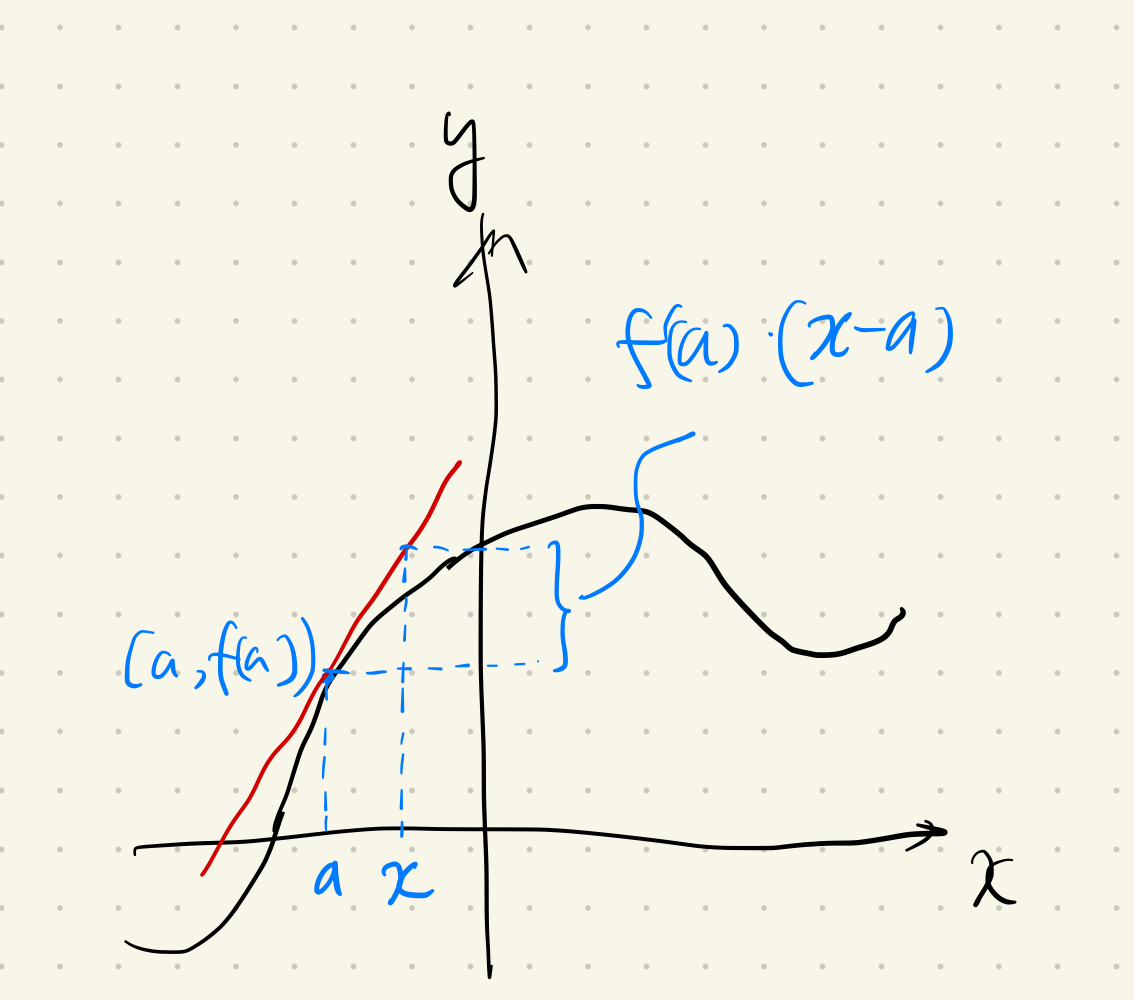
\includegraphics[width = 0.7\textwidth]{figures/chap 05/lin_approx_intro.png}
    \label{fig: lin_approx_intro}
\end{figure}

Since the curve is very close to the tangent line when $x$ is close to $a$, we can \textit{approximate} the values of $f(x)$ at $x \approx a$ with $\hat{f}(x) \approx f(a) + f'(a)(x-a)$.  In fact, one can prove that $\hat{f}(x)$ is the "best linear approximant" to $f(x)$ near $x=a$ by showing that any other linear approximant has a relatively larger error when $x \rightarrow a$.  To see this, say there is another linear approximant $f^*(x) = q + p(x-a)$, then ratio of the approximation errors between $\hat{f}(x)$ and $f^*(x)$ can be written as:

\[\frac{f(x)-\hat{f}(x)}{f(x) - f^*(x)} = \frac{f(x)-[f(a)+f'(a)(x-a)]}{f(x)-[q+p(x-a)]}\]

Taking the limit where $x \rightarrow a$, we yield:

\begin{align}
    &\lim\limits_{x \to a} \frac{f(x)-\hat{f}(x)}{f(x) - f^*(x)} \nonumber \\
    =&\lim\limits_{x \to a} \frac{f(x)-[f(a)+f'(a)(x-a)]}{f(x)-[q+p(x-a)]} \nonumber \\
    =&\lim\limits_{x \to a} \frac{[f(x)-f(a)]-f'(a)(x-a)}{[f(x)-f(a)]-[(q-f(a))+p(x-a)]} \label{eqn: lin_approx_best_1}\\
    =&\lim\limits_{x \to a} \frac{\frac{f(x)-f(a)}{x-a}-f'(a)}{\frac{f(x)-f(a)}{x-a}-\left[\frac{q-f(a)}{x-a}+p\right]}\label{eqn: lin_approx_best_2}
\end{align}

Now we have two cases:

\begin{enumerate}[(a)]
    \item If $q \ne f(a)$, then from (\ref{eqn: lin_approx_best_1}):\\
    \[\lim\limits_{x \to a} \frac{[f(x)-f(a)]-f'(a)(x-a)}{[f(x)-f(a)]-[(q-f(a))+p(x-a)]} = \frac{0-0}{0-[(q-f(a))-0]} = 0\]
    where $f(x)-f(a) = 0$ since $f(x)$ is differentiable at $x=a$ and thus continuous there.
    \item If $q = f(a)$ but $p \ne f'(a)$, then from (\ref{eqn: lin_approx_best_2}):\\
    \[\lim\limits_{x \to a}\frac{\frac{f(x)-f(a)}{x-a}-f'(a)}{\frac{f(x)-f(a)}{x-a}-\left[\frac{q-f(a)}{x-a}+p\right]} = \frac{f'(a)-f'(a)}{f'(a)-[0 + p]} = 0\]
\end{enumerate}

Therefore, the error ratio goes to zero if $f^*(x)$ is not $\hat{f}(x)$, which implies that the tangent line approximant has a smaller error than any other linear approximants as $x \rightarrow a$.  We write this as a theorem:

\pagebreak

\begin{theo}[Linear approximation of general function]{thm: lin_approx}
    Suppose $f(x)$ is differentiable at $x=a$, then the best linear approximant for $f(x)$ at $x=a$ is
    \[\hat{f}(x) = f(a)+f'(a)(x-a)\]
\end{theo}

The advantage of using linear approximations is that when $f(x)$ is complicated and difficult evaluate, $\hat{f}(x) = f(a) + f'(a)(x-a)$ may be relatively easy to calculate.  We will demonstrate in the following example:


\begin{eg}[]{eg: lin_approx_sqrt}
    Give an approximate value for $\sqrt{1.0003}$ using linear approximation.
\end{eg}

\begin{egsol}[]{egsol: lin_approx_sqrt}
    $\sqrt{1.0003}$ may be hard to compute, yet $\sqrt{1}$ is trivial.  Therefore, we define a function $f(x) = \sqrt{x}$ so that $f(1.0003) = \sqrt{1.0003}$.  We can then obtain the linear approximation of $f(x)$ at $x=1$ to help us approximate $f(1.0003)$.  Using the power rule, $f'(x) = \frac{1}{2\sqrt{x}}$, so we have our linear approximant:
    \[\hat{f}(x) = f(1) + f'(1)(x-1) = \sqrt{1} + \frac{1}{2\sqrt{1}}(x-1) = 1+\frac{x-1}{2}\]
    Therefore, the linear approximation of $\sqrt{1.0003}$ would be:
    \[\sqrt{1.0003} = f(1.0003) \approx \hat{f}(1.0003) = 1+\frac{0.0003}{2} = 1.00015\]
    Note that the true value of $\sqrt{1.0003}$ is $1.0001499887...$, so our approximation is acutally quite good.
\end{egsol}

\begin{remark}
    Note that we based our linear approximation at $x=1$ instead of, say, $x=0.5$ for two reasons: (a) $f(0.5)$ and $f'(0.5)$ are not as easily computed as $f(1)$ and $f'(1)$, (b) $1.0003$ is closer to $1$ than $0.5$, so the approximant at $x=1$ would perform better than the approximant at $x=0.5$.
\end{remark}

\begin{ex}[]{ex: lin_approx_cbrt}
Give an approximate value for $\sqrt[3]{65}$ using linear approximation.
\end{ex}

\begin{exsol}[]{exsol: lin_approx_cbrt}
We can rewrite $\sqrt[3]{65}$ as:
\[\sqrt[3]{65} = \sqrt[3]{64 + 1} = \sqrt[3]{64\left(1+\frac{1}{64}\right)}= 4\sqrt[3]{1+\frac{1}{64}}\]
While $\sqrt[3]{1+\frac{1}{64}}$ is difficult to evaluate, we actually can compute $\sqrt[3]{1}$ quite easily.  So we let $f(x) = \sqrt[3]{x}$ and find its linear approximant at $x=1$. Since $f'(x) = \frac{1}{3}x^{-\frac{2}{3}} = \frac{1}{3\big(\sqrt[3]{x}\big)^2}$, we have,
\[\hat{f}(x) = f(1) + f'(1)(x-1) = \sqrt[3]{1} + \frac{1}{3\big(\sqrt[3]{1}\big)^2}(x-1) = 1+\frac{x-1}{3}\]
Therefore, the linear approximation for $\sqrt[3]{65}$ would be,
\[\sqrt[3]{65} = 4f\Big(1+\frac{1}{64}\Big) \approx 4\hat{f}\Big(1+\frac{1}{64}\Big) = 4\Big(1+\frac{1/64}{3}\Big) = 4+\frac{1}{48} \approx 4.02083\]
The true value of $\sqrt[3]{65}$ is actually about 4.02072, so we are precise to the third decimal using linear approximation.
\end{exsol}

\subsection{Linear Approximation of Common Functions}
In the following we try to derive a list of linear approximants for common functions.  Note that we rewrite the form for some of the functions so that all the the approximants are expanded at $x=0$, so that

\[f(x) \approx \hat{f}(x) = f(0)+f'(0)x\]
\begin{table}[ht]
    \centering
    \begin{tabular}{ccccc}
        $f(x)$ & $f'(x)$ & $f(0)$ & $f'(0)$ & $\hat{f}(x)$\\
        \hline
        $(1+x)^r$ & $r(1+x)^{r-1}$ & $1$ & $r$ & $1+rx$ \\
        $e^x$ & $e^x$ & $1$ & $1$ & $1+x$ \\
        $\ln(1+x)$ & $\frac{1}{1+x}$ & $0$ & $1$ & $x$ \\
        $\sin x$ & $\cos x$ & $0$ & $1$ & $x$ \\
        $\cos x$ & $-\sin x$ & $1$ & $0$ & $1$
    \end{tabular}
    \label{tab: lin_approx_deriv}
\end{table}

We summarize the results into the following theorem:

\pagebreak

\begin{theo}[Linear approximation of common functions]{thm: lin_approx_fxn}
    When $x \approx 0$, we have the following linear approximations:
    \[(1+x)^r \approx 1+rx \qquad e^x \approx 1+x \qquad \ln(1+x) \approx x \qquad \sin x \approx x \qquad \cos x \approx 1 \]
\end{theo}

\begin{remark}
    These approximations tells us the behavior of these functions near $x=0$. Eg. $\sin x$ behaves like $x$ (linearly) when $x$ is near zero.  This can also be seen on the graph:
\end{remark}

\begin{figure}[ht]
    \centering
    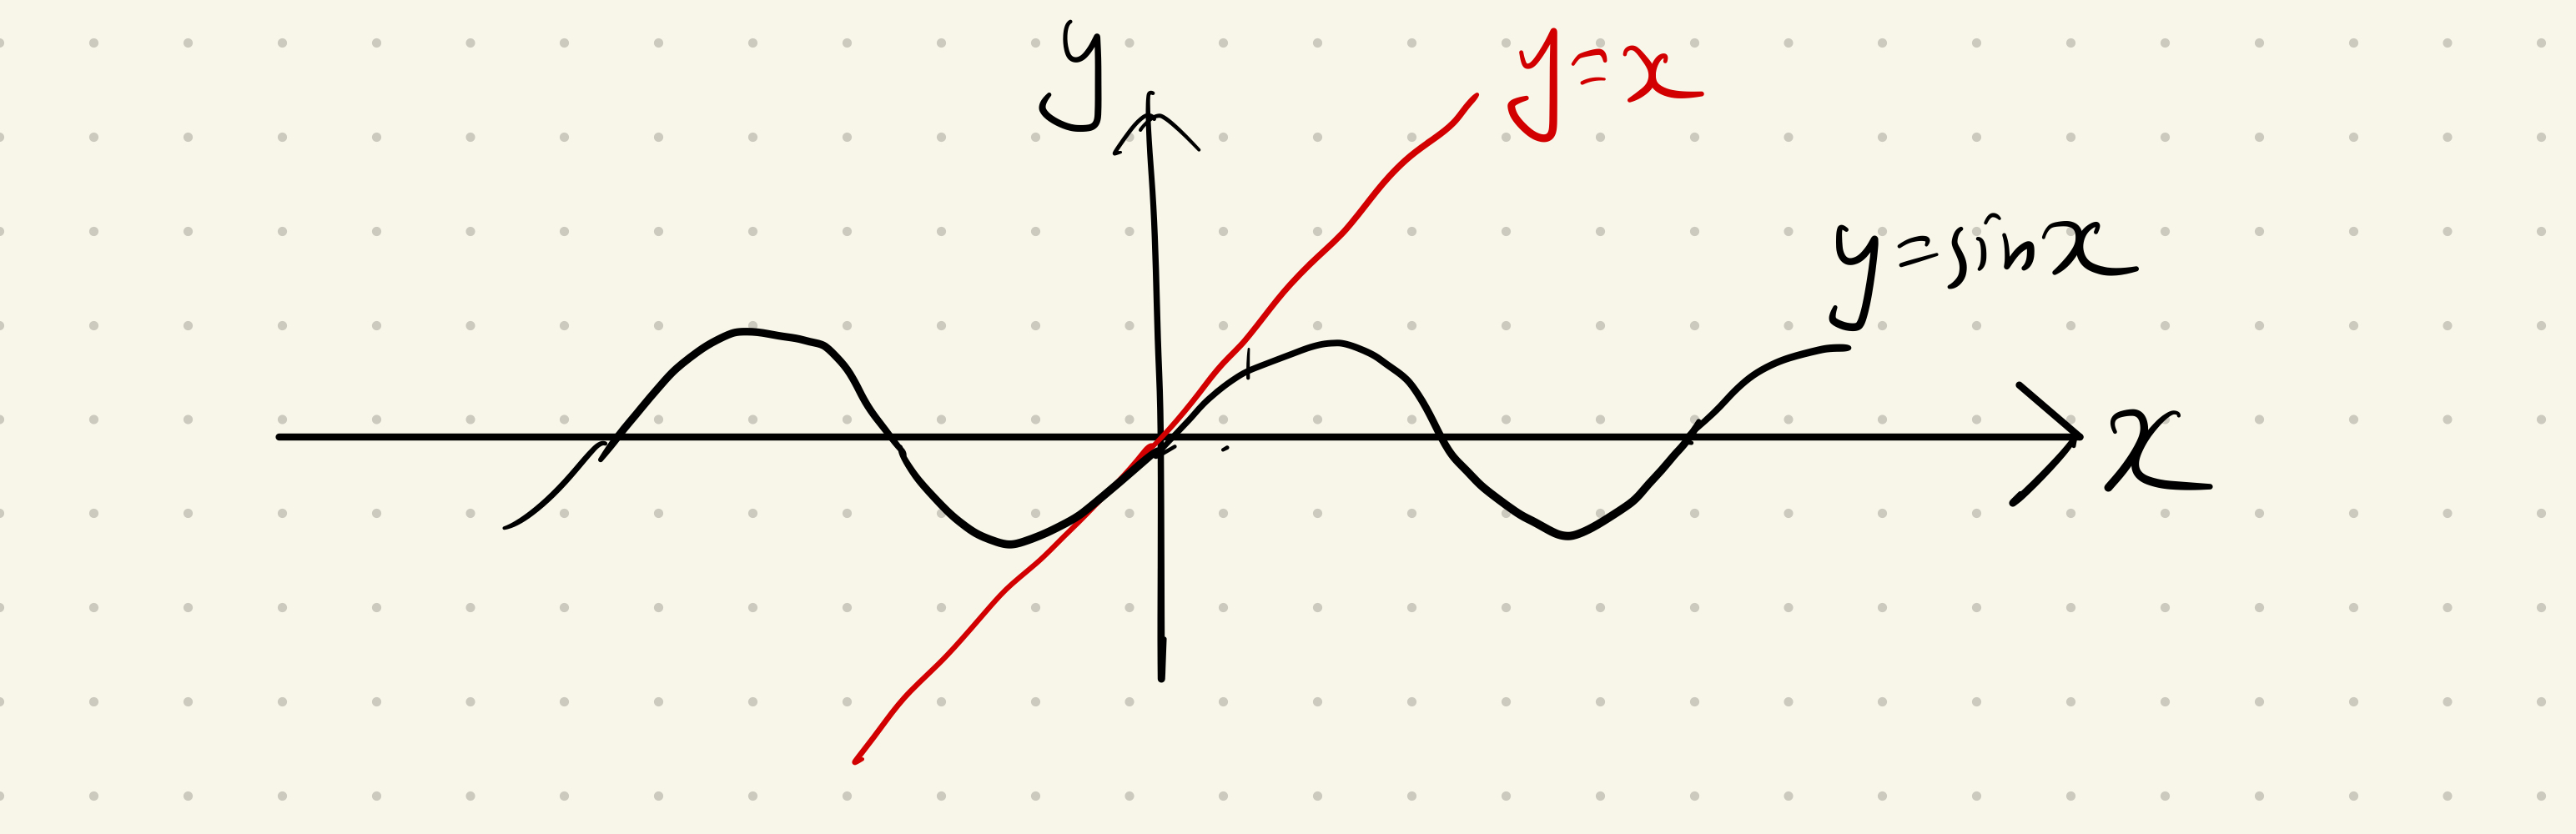
\includegraphics[width = 0.7\textwidth]{figures/chap 05/lin_approx_sin.png}
    \label{fig: lin_approx_sin}
\end{figure}

\begin{remark}
    The approximant for $\cos x$ seems weird: there is no $x$ in the approximant!  This indicates that when restricting to linear approximation, the behavior of $\cos x$ near $x=0$ is best approximated with a horizontal line, as shown in the graph:
\end{remark}

\begin{figure}[ht]
    \centering
    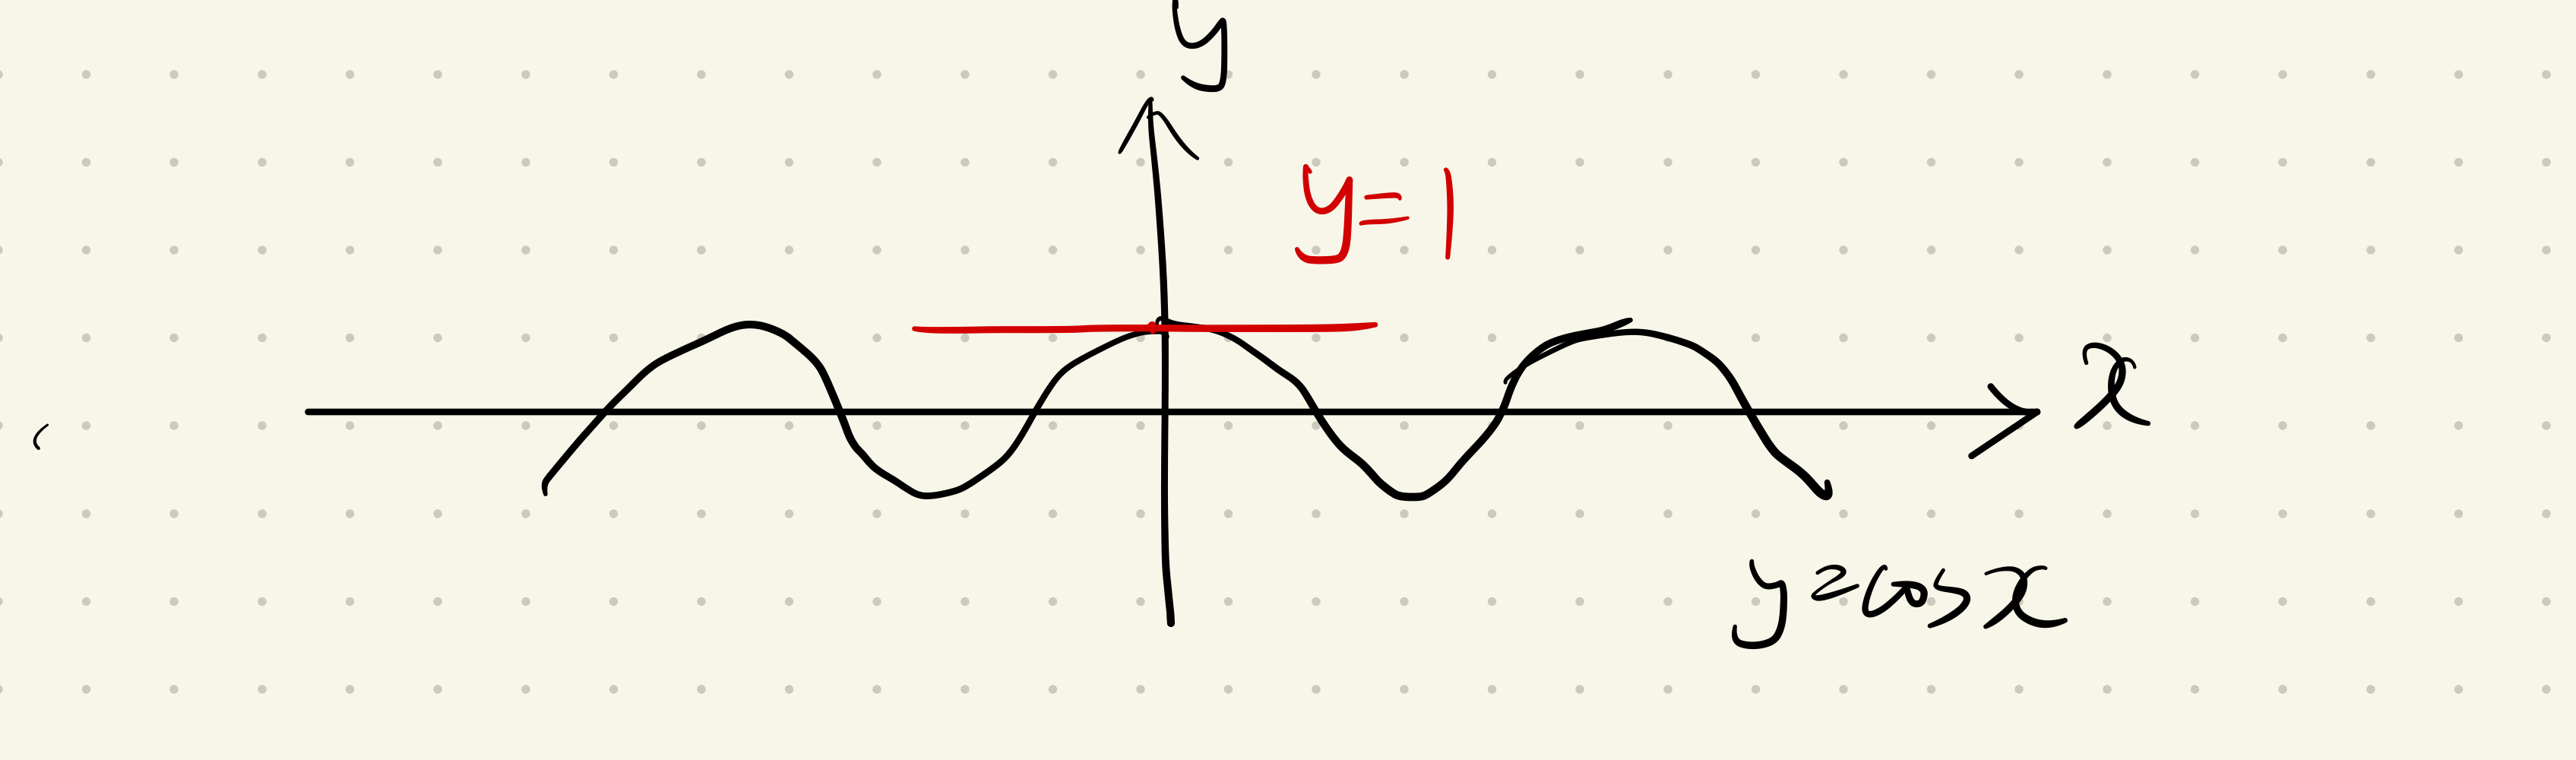
\includegraphics[width = 0.7\textwidth]{figures/chap 05/lin_approx_cos.png}
    \label{fig: lin_approx_cos}
\end{figure}

When functions are added / subtracted / multiplied with each other, we can do approximations to the individual functions first, then perform teh addtition / subtraction / multiplication.  We will demonstrate this in the following example.

\begin{eg}[]{eg: lin_approx_comb}
    Find the linear approximant to $f(x) = \frac{2e^x + \ln(1+x)}{\sqrt{1+x}}$ at $x = 0$.
\end{eg}

\begin{egsol}[]{egsol: lin_approx_comb}
    If we try to approximate $f(x)$ at $x=0$ with the tangent line formula, we first need to find its derivative with the quotient rule:
    \[f'(x) = \frac{\big(2e^x + \frac{1}{1+x}\big)\sqrt{1+x} - [2e^x + \ln(1+x)]\frac{1}{\sqrt{1+x}}}{\big(\sqrt{1+x}\big)^2}\]
    Therefore we have
    \[f(0) = \frac{2+0}{\sqrt{1}} = 2\]
    \[f'(0) = \frac{(2+1)\sqrt{1+0}-[2+0]\frac{1}{2\sqrt{1}}}{\big(\sqrt{1+0}\big)^2} = \frac{3-1}{1} = 2\]
    And the approximant is 
    \[\hat{f}(x) = f(0) + f'(0)(x-0) = 2+2x\]
    Alternatively, we can approximate first and get
    \begin{align*}
        f(x) &= [2e^x + \ln(1+x)](1+x)^{-\frac{1}{2}}\\
        &\approx [2(1+x) + x]\Big(1-\frac{1}{2}x\Big)\\
        &=[2+3x]\Big(1-\frac{1}{2}x\Big)\\
        &=2+2x-\frac{3}{2}x^2 \approx 2+2x
    \end{align*}
    The last approximation discards the $x^2$ term since when $x$ is near $0$, $x^2$ is negligible compared to $x$.  We can see that these two approaches yield identical results.
\end{egsol}

We will conclude linear approximations with an exercise:

\begin{ex}[]{ex: lin_approx_comb}
    Find the linear approximant to $f(x) = 3xe^{2x-10}$ at $x = 5$.
\end{ex}

\begin{exsol}[]{exsol: lin_approx_comb}
    (Approach 1) 
    
    We use the tangent line formula directly, so we first obtain the derivative of $f(x)$ 
    \[f'(x) = 3e^{2x-10} + 3xe^{2x-10}\cdot 2 = (6x+3)e^{2x-10}\]
    Therefore,
    \[f(5) = 3 \cdot 5 \cdot e^0 = 15\]
    \[f'(5) = (6 \cdot 5+3)e^0 = 33\]
    And the linear approximant is
    \[\hat{f}(x) = f(5) + f'(5)(x-5) = 15 + 33(x-5) = 33x-150\]
    
    (Approach 2)
    
    Let $x = 5 + \delta$, then when $x \approx 5$, $\delta \approx 0$, and we have
    
    \begin{align*}
        f(x) &= 3(5+\delta)e^{2(5+\delta)-10}\\
        &=3(5+\delta)e^{2\delta}\\
        &\approx3(5+\delta)(1+2\delta)\\
        &=15+33\delta+6\delta^2\\
        &\approx 15+33\delta = 15+33(x-5) = 33x-150
    \end{align*}
    
    The two approaches still yield the same linear approximant.
\end{exsol}

\subsection{Quadratic Approximation and Beyond}
Previously we used linear approximation to approximate $\cos x$ near $x=0$ and got $\cos x \approx 1$, which is somewhat anticlimactic.

\begin{figure}[ht]
    \centering
    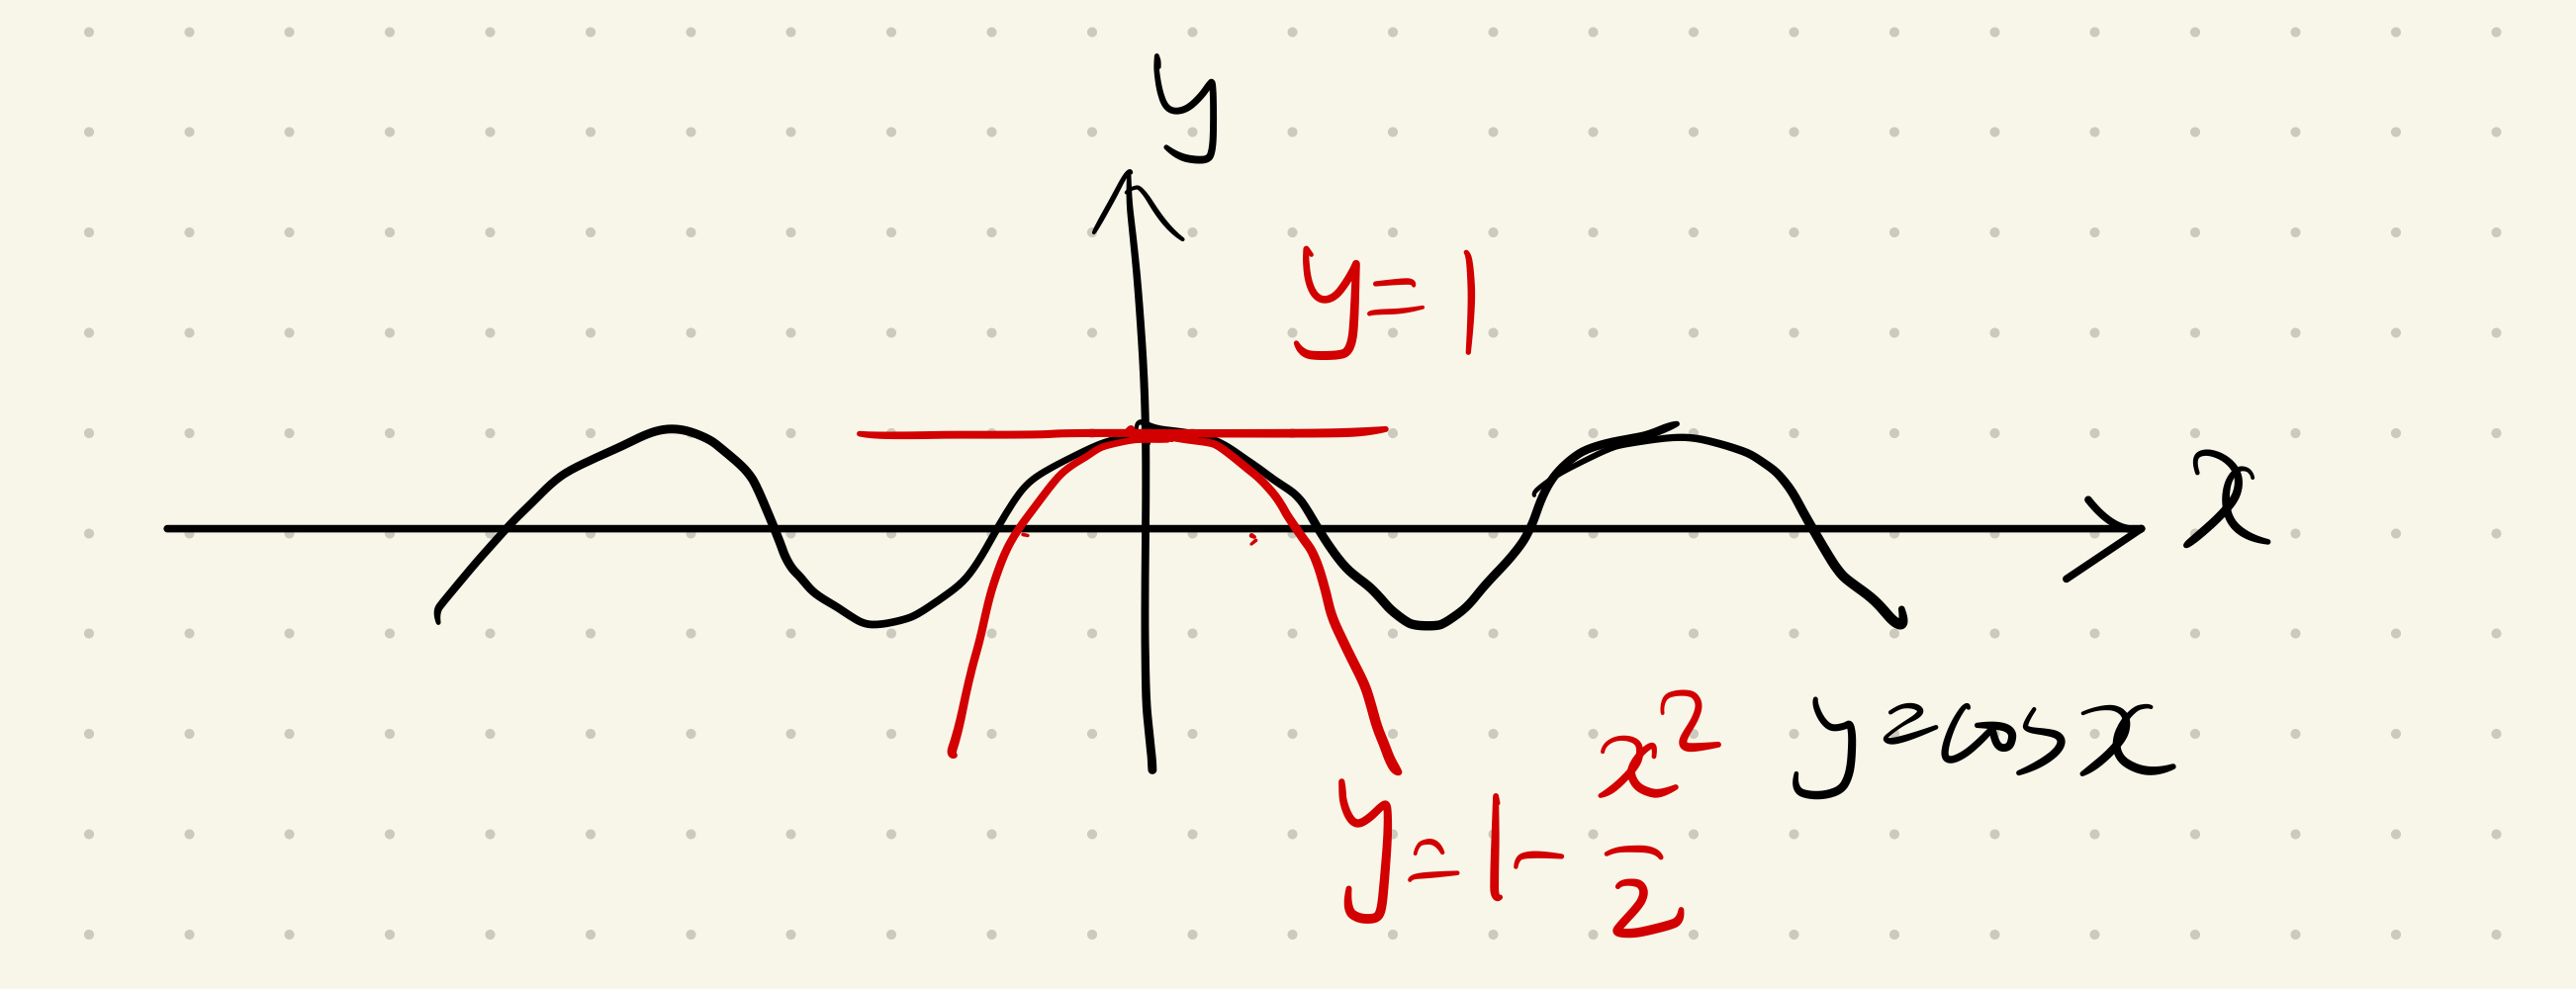
\includegraphics[width = 0.7\textwidth]{figures/chap 05/qua_approx_cos.png}
    \label{fig: qua_approx_cos}
\end{figure}

As shown in the graph above, although $y=1$ is the best line that approximates the behavior of $\cos x$ near zero, it is not doing a good job when $x$ is a bit far from zero.  A possible improvement is to use a degree-$2$ polynomial (parabola) instead of a degree-$1$ polynomial (line) to do the approximation, so that the approximant can curve and fit $\cos x$ better.

Suppose we want to approximate our desired function $f(x)$ near $x=a$.  Before we get to degree-$2$ polynomials, we first observe that if we write the degree-$1$ polynomial approximant as $\hat{f}_1(x) = b_0 + b_1(x-a)$, then matching the function value and derivative at $x=a$, i.e. letting $f(a) = \hat{f}_1(a)$ and $f'(a) = \hat{f}'_1(a)$, will give us the best solution $f(a) + f'(a)(x-a)$, as shown in the following table:

\begin{table}[ht]
    \centering
    \begin{tabular}{cccc}
        &Original function & Linear approximant & Quadratic approximant \\
        &$f(x)$ & $\hat{f}_1(x) = b_0+b_1(x-a)$ &  $\hat{f}_2(x) = b_0+b_1(x-a)+b_2(x-a)^2$ \\
        \hline
        Value @ $x=a$ & $f(a)$ & $b_0$ & $b_0$\\
        Derivative @ $x=a$ & $f'(a)$ & $b_1$ & $b_1$\\
        $2^{nd}$ derivative @ $x=a$ & $f''(a)$ & $0$ & $2b_2$
    \end{tabular}
    \label{tab: qua_approx}
\end{table}

Likewise, if we write the degree-$2$ polynomial approximant as $\hat{f}_2(x) = b_0 + b_1(x-a) + b_2(x-a)^2$, we can find the best solution by letting $f(a) = \hat{f}_2(a)$, $f'(a) = \hat{f}'_2(a)$ and $f''(a) = \hat{f}''_2(a)$. This leads to $b_0 = f(a)$, $b_1 = f'(a)$ and $b_2 = \frac{1}{2}f''(a)$, and we have the following theorem:

\begin{theo}[Quadratic approximation of general function]{thm: qua_approx}
    Suppose $f(x)$ is twice differentiable at $x=a$, then the best quadratic approximant for $f(x)$ at $x=a$ is 
    \[\hat{f}(x) = f(a)+f'(a)(x-a)+\frac{1}{2}f''(a)(x-a)^2\]
\end{theo}

We can then list some quadratic approximants for common functions:

\begin{table}[ht]
    \centering
    \begin{tabular}{ccccccc}
        $f(x)$ & $f'(x)$ & $f''(x)$ & $f(0)$ & $f'(0)$ & $f''(0)$ &$\hat{f}(x)$\\
        \hline
        $(1+x)^r$ & $r(1+x)^{r-1}$ & $r(r-1)(1+x)^{r-2}$ & $1$ & $r$ & $r(r-1)$ & $1+rx+\frac{r(r-1)}{2}x^2$ \\
        $e^x$ & $e^x$ & $e^x$ & $1$ & $1$ & $1$ & $1+x+\frac{1}{2}x^2$ \\
        $\ln(1+x)$ & $\frac{1}{1+x}$ & $-\frac{1}{(1+x)^2}$ & $0$ & $1$ & $-1$ & $x-\frac{1}{2}x^2$ \\
        $\sin x$ & $\cos x$ & $-\sin x$ & $0$ & $1$ & $0$ & $x$\\
        $\cos x$ & $-\sin x$ & $-\cos x$ & $1$ & $0$ &$-1$ & $1-\frac{1}{2}x^2$
    \end{tabular}
    \label{tab: qua_approx_deriv}
\end{table}

We summarize the results into the following theorem:

\begin{theo}[Quadratic approximation of common functions]{thm: qua_approx_fxn}
    When $x \approx 0$, we have the following quadratic approximations:
    \[(1+x)^r \approx 1+rx+\frac{r(r-1)}{2}x^2 \qquad e^x \approx 1+x+\frac{x^2}{2} \qquad \ln(1+x) \approx x-\frac{x^2}{2}\]
    \[\sin x \approx x \qquad \cos x \approx 1-\frac{x^2}{2} \]
\end{theo}

\begin{remark}
    Notice that our quadratic approximant for $\cos x$ near $x=0$ performs much better than the linear approximant, especially when $x$ is a bit away from $0$, as shown in the graph above.  Also, the quadratic approximant for $\sin x$ near $x=0$ is the same as its linear approximant, which implies that introducing an extra $x^2$ term does not improve the approximation of $\sin x$ near $x=0$.
\end{remark}

In fact, by the virtue of linear and quadratic approximants, if we try to approximate $f(x)$ near $x=c$ with higher order polynomials by matching an array of high-order derivatives at $x=c$, eventually we will get the famous \textit{Taylor series}:

\[\sum_{n=0}^\infty\frac{f^{(n)}(a)}{n!}(x-a)^n = f(a) + f'(a)(x-a) + \frac{f''(a)}{2!}(x-a)^2 + \frac{f'''(a)}{3!}(x-a)^3 + \cdots\]

Under certain conditions (which we will not dig further into for now), this series is actually an accurate representation for $f(x)$.  In other words, it is no longer an approximation to $f(x)$: it \textit{is} $f(x)$.  We provide some of the famous Taylor series below:

\begin{theo}[Taylor series of common functions]{thm: taylor_fxn}
    \vspace{-0.5cm}
    \begin{align*}
        e^x &= 1 + x + \frac{x^2}{2!} + \frac{x^3}{3!} + \frac{x^4}{4!} + \cdots\\
        \sin x &= x - \frac{x^3}{3!} + \frac{x^5}{5!} - \frac{x^7}{7!} + \cdots\\
        \cos x &= 1 - \frac{x^2}{2!} + \frac{x^4}{4!} - \frac{x^6}{6!} + \cdots\\
        \ln(1+x) &= x - \frac{x^2}{2} + \frac{x^3}{3} - \frac{x^4}{4!} + \cdots \qquad (-1 < x \le 1)\\
        \frac{1}{1-x} &= 1 + x + x^2 + x^3 + x^4 + \cdots \qquad (-1 < x < 1)
    \end{align*}
\end{theo}

To digress a little bit, although in this course we only talk about real numbers, but if we define $i = \sqrt{-1}$ as the imaginary square root of $-1$ and plug $ix$ into the Taylor series for $e^x$, we get

\begin{align*}
    e^{ix} &= 1+ix+\frac{(ix)^2}{2!} + \frac{(ix)^3}{3!} + \frac{(ix)^4}{4!} + \frac{(ix)^5}{5!} + \frac{(ix)^6}{6!} - \frac{(ix)^7}{7!} + \cdots \\
    &= 1+ix-\frac{x^2}{2!} - \frac{ix^3}{3!} + \frac{x^4}{4!} + \frac{ix^5}{5!} - \frac{x^6}{6!} + \frac{ix^7}{7!} + \cdots \\
    &= \left(1 - \frac{x^2}{2!} + \frac{x^4}{4!} - \frac{x^6}{6!} + \cdots\right) + i\left(x - \frac{x^3}{3!} + \frac{x^5}{5!} - \frac{x^7}{7!} + \cdots\right)\\
    &= \cos x + i \sin x
\end{align*}

which is a remarkable result proposed (popularized) by the famous mathematician \textit{Leonhard Euler} (1707-1783).  In addition, pluggin $\pi$ into $x$ and we yield $e^{i\pi} = -1$. Or, even better,
\[e^{i\pi}+1 = 0\]
This formula, also termed as \textit{Euler's identity}, is considered as the most beautiful formula by some, since it relates five of the fundamental numbers in mathematics: $e$, $\pi$, $i$, $1$, $0$, all in a compact and simple formula.
\newpage

\section{Newton's Method}
Derivatives are also useful in finding roots of a function $f(x)$, i.e. finding $x$ where $f(x) = 0$.  Sometimes you \textit{can} find the roots by simply solving $f(x)=0$ on paper, but for complicated functions (eg. $f(x) = x^2 - \sin x$) you have to resort to numerical methods, which approximate the roots using iterative procedures.  Newton's method is one of the numerical methods that has a fairly fast speed of convergence (i.e. it can get you a pretty accurate answer within a few iterations).

For example, suppose we want to find the roots of $f(x) = x^2-3$.  In this case, we know its roots are $\pm \sqrt{3}$ by solving $x^2-3 = 0$, but we now try to find the roots numerically.  To initiate Newton's method, we must first guess a solution that is not too far off.  We notice $f(1) = -2 < 0$ and $f(2) = 1 > 0$, so there is (probably) a root between $1$ and $2$.  Let's make a initial guess of $1$.  Since this is our initial guess, we denote it as $x_0 = 1$.  This gives us a graph a follows:

\begin{figure}[ht]
    \centering
    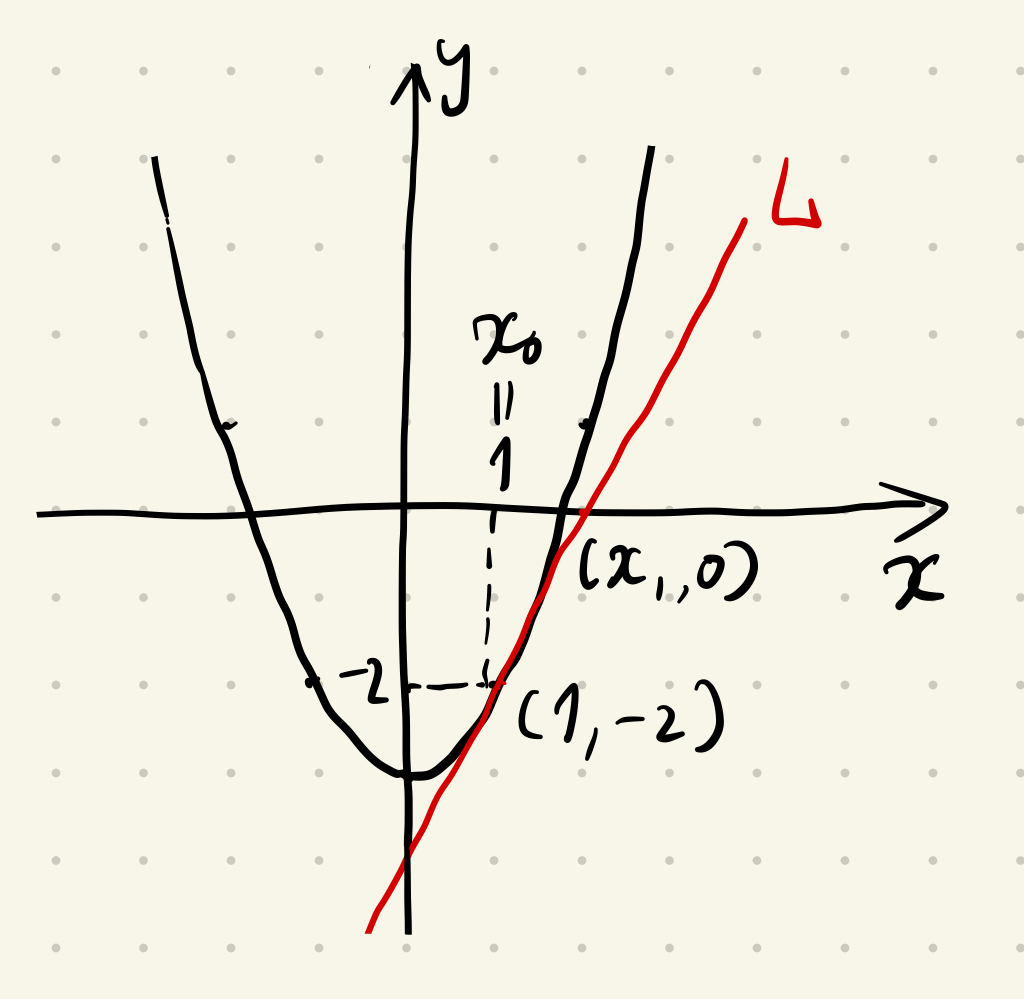
\includegraphics[width = 0.5\textwidth]{figures/chap 05/newton_1.png}
    \label{fig: newton_1}
\end{figure}

We see that our guess of $x_0 = 1$ is not quite correct since $f(x_0) = -2$.  However, from this point on the curve we can construct a tangent line $L$ that intersects with the $x$-axis at $(x_1, 0)$.  The mindset is that if $L$ is a good linear approximation to $f(x)$ near $x = 1$, then $(x_1, 0)$ should be very close to the point where the curve intersects the $x$-axis.  Knowing that $f'(x) = 2x$, we can express $L$ using our tangent line formula (or linear approximation formula, if you will):
\[L: y = -2 + 2(x-1) = 2x-4\]
Since $L$ passes through $(x_1, 0)$, the following equation should be satisfied: 
\[0 = 2x_1-4\]
So we get our next guess $x_1 = 2$, which still isn't quite right since $f(2) = 1$.  We can apply the same trick again, i.e. do another iteration of Newton's method based on the following graph (which is scaled and a little distorted for demonstration):

\begin{figure}[ht]
    \centering
    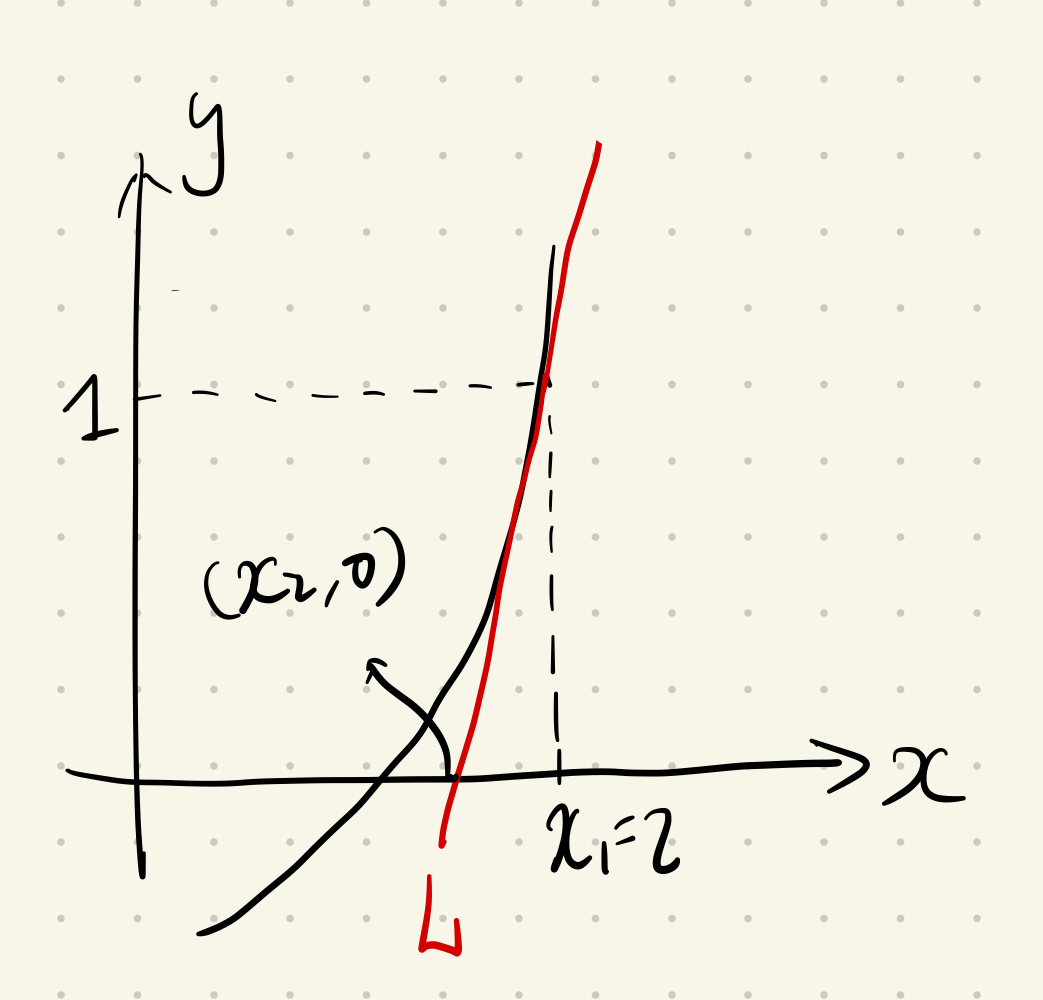
\includegraphics[width = 0.5\textwidth]{figures/chap 05/newton_2.png}
    \label{fig: newton_2}
\end{figure}

The equation for the new tangent line, which passes through $(2, f(2) = 1)$, is
\[L: y = 1 + 4(x-2) = 4x-7\]
using the fact that $f'(2) = 2 \cdot 2 = 4$.  Following the same procedure, we aim to find the point where $L$ intersects with the $x$-axis, $(x_2, 0)$.  Since $L$ passes through $(x_2, 0)$, we have
\[0 = 4x_2-7\]
So we have our next guess $x_2 = \frac{7}{4}$.  Now you can see that $f\big(\frac{7}{4}\big) = 0.0625$, which is really close to $0$, so we're very close to our solution.  In practice, we can set a small positive number $\epsilon$ (sometimes termed as \textit{tolerance}) that stands for the maximum error magnitude in function value we are willing to accept, then repeat the iterations until $|f(x_k)| < \epsilon$ and claim $x_k$ is our approximated root and call it a day.  If we set the tolerance as $10^{-8}$, then we only need $4$ iterations to arrive at our answer:

\begin{table}[ht]
    \centering
    \begin{tabular}{cccc}
        Iteration number & Root estimate & Error in function value & Error of estimate\\
        ($k$) & ($x_k$) & ($f(x_k)$) & ($x_k - \sqrt{3}$)\\
        \hline
        $0$ & $1$ & $-2$ & $-0.7321$\\
        $1$ & $2$ & $1$ & $0.2679$\\
        $2$ & $7/4$ & $0.0625$ &  $0.0179$\\
        $3$ & $97/56$ & $3.19\times 10^{-4}$ & $9.20 \times 10^{-5}$\\
        $4$ & $18817/10864$ & $8.47\times 10^{-9}$ & $2.45 \times 10^{-9}$
    \end{tabular}
    \label{tab: newton_iteration}
\end{table}

\begin{remark}
    The iteration is actually going closer and closer to one of the roots, $\sqrt{3}$, but does not get anywhere near the other root, $-\sqrt{3}$.  To find the other root, we will have to pick an initial value closer to $-\sqrt{3}$, eg. $x_0 = -1$.
\end{remark}

Note that although Newton's methods is quite powerful, in some cases it will fail miserably.  One of the failure modes is when Newton's method iterates to a point where the derivative is zero.  For example, if we make our initial guess of $x_0 = 0$, then $f'(x_0) = 0$, so the tangent line $L$ is horizontal and does not intersect with the $x$-axis and we do not know how to make the next guess $x_1$. 

Another failure mode of Newton's method is when the root estimate jumps between several points and does not converge.  For example, in the following figure, if you initialize at $x = x_0$, the next guess would be $x = x_1$.  Yet in the next iteration, plugging in $x_1$ will lead you back to $x_0$, and you will get nowhere near the true root $x^*$.  The two failure modes mentioned above can be circumvented by choosing a better initial guess of $x_0$.  

\begin{figure}[ht]
    \centering
    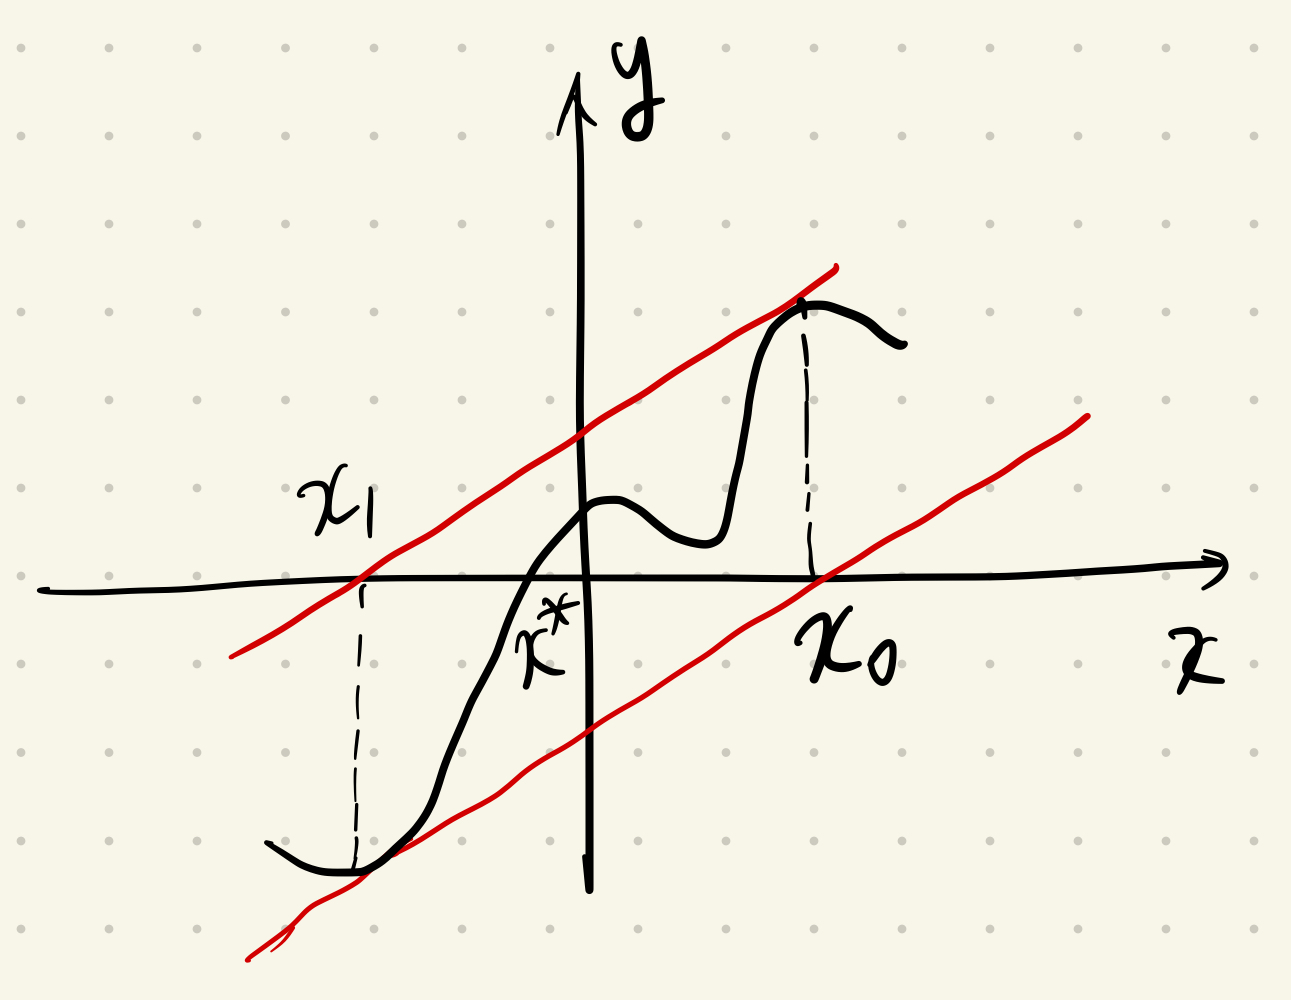
\includegraphics[width = 0.5\textwidth]{figures/chap 05/newton_3.png}
    \label{fig: newton_3}
\end{figure}

There are still other failures modes for Newton's method, but we will not discuss further: just keep in mind that if Newton's method is taking a lot of iterations and does not seem to be converging, you may have encountered a case where Newton's method fails.  You should try changing your initial guess or opting for another root-finding algorithm.

Lastly, we derive the general formula for each iteration of Newton's method.  Suppose we are finding the roots of $f(x)$, and our current guess is $x_k$, the tangent line over $(x_k, f(x_k))$ is:
\[L: y = f(x_k) + f'(x_k)(x-x_k)\]
The next guess for the root, $x_{k+1}$, is the $x$-coordinate of intersection point between $L$ and the $x$-axis, i.e. $L$ passes through $(x_{k+1}, 0)$.  So we have
\[0 = f(x_k) + f'(x_k)(x_{k+1}-x_k)\]
Rearrange the equation and we get the following theorem:

\newpage

\begin{theo}[Iteration formula for Newton's method]{thm: newton}
    Let $x_k$ be root estimate for $f(x)$ from the $k^{\text{th}}$ iteration in Newton's method, then the root estimate of the next iteration, $x_{k+1}$, can be found by
    \[x_{k+1} = x_k - \frac{f(x_k)}{f'(x_k)}\]
\end{theo}

From this formula, you can see that the failure mode where the derivative is zero becomes evident, since zero would then be in the denominator and the procedure does not make sense.  We will end this section with an exercise.

\begin{ex}[]{ex: newton}
    Approximate the value of $\sqrt[3]{2}$ by finding the root of $f(x) = x^3 - 2$ with Newton's method.
\end{ex}

\begin{exsol}[]{exsol: newton}
    First, we obtain the derivative of $f(x)$, which is $f'(x) = 3x^2$.  The iteration formula is then
    
    \[x_{k+1} = x_k-\frac{x_k^3-2}{3x_k^2}\]
    
    Now we must make an initial guess, $x_0$, for the root of $f(x)$.  Since we know that $f(1) = -1 < 0$ and $f(2) = 6 > 0$, we reckon that there should be a root for $f(x)$ between $1$ and $2$, and we set $x_0 = 1$ for convenience.  We also set the tolerance $\epsilon$ to be $10^{-4}$.
    
    \vspace{0.3cm}
    
    \begin{center}
        \begin{tabular}{ccc}
            Iteration number & Root estimate & Error in function value\\
            $(k)$ & $\Big(x_k = x_{k-1}-\frac{x_{k-1}^3-2}{3x_{k-1}^2}\Big)$ & $(x_k^3-2)$\\
            \hline
            $0$ & $1$ & $-1$\\
            $1$ & $4/3$ & $0.370$\\
            $2$ & $91/72$ & $0.0190$\\
            $3$ & $1126819/894348$ & $5.93\times 10^{-5}$
        \end{tabular}
    \end{center}
    
    We thus have our estimate $x_3 = \frac{1126819}{894348} \approx 1.2599335$.  
    
    Compared to the true root $\sqrt[3]{2} \approx 1.2599210$, we are accurate to the fourth decimal.  Actually, if we lower our tolerance and allow one more iteration, we can be accurate to the seventh decimal.
    \label{tab: newton_iteration_ex}
\end{exsol}

\newpage
\section{Related Rates}
In some application problems, we known the relationship between two or more variables, eg. price and demand of a product; volume, surface area and radius of a ball.  Since these variables are inter-related, if one variable is changing with time at a certain rate, the other variables will also be changing with time based on the given relationship, and its rate of change can be deduced using derivatives.  In these types of problems, implicit differentiation will come in handy frequently.  To see this, let us look at the following examples:

\begin{eg}[]{eg: related_rates_balloon}
    An air nozzle is blowing air into the balloon at the speed of $150\text{ cm}^3/\text{sec}$. Suppose we can treat the balloon as a perfect sphere and the balloon is now $10$ cm in diameter.  How fast is the diameter of the balloon growing right now? 
\end{eg}

\begin{egsol}[]{egsol: related_rates_balloon}
    If we denote the diameter of the balloon as $D$ (cm) and its volume as $V$ (cm$^3$), then we can relate them with the following equation:
    \[V =\frac{4}{3}\pi \Big(\frac{D}{2}\Big)^3 = \frac{\pi}{6}D^3\]
    To obtain the related rates between $V$ and $D$, we differentiate both sides of the equation by time $t$ (measured in seconds).  Note that $V$ and $D$ are both functions of $t$, so we need to use the chain rule along the way:
    \begin{align*}
        \frac{d}{dt}V &= \frac{d}{dt}\Big(\frac{\pi}{6} D^3\Big)\\
        \frac{dV}{dt} &= \frac{\pi}{6}\frac{dD^3}{dt} = \frac{\pi}{6}\frac{dD^3}{dD}\frac{dD}{dt} = \frac{\pi}{6}\cdot 3D^2 \frac{dD}{dt} = \frac{\pi}{2} D^2 \frac{dD}{dt}
    \end{align*}
    Or we may use the Lagrange notation, defining $()'$ as differentiating with respect to $t$:
    \[V' = \Big(\frac{\pi}{6} D^3\Big)' = \frac{\pi}{6}(D^3)' = \frac{\pi}{6}\cdot 3D^2 \cdot D' = \frac{\pi}{2} D^2D'\]
    Since the nozzle is blow air at the speed of $150\text{cm}^3/\text{sec}$ and the balloon is currently $10$cm in diameter, we have $V' = 150$ and $D = 10$, so 
    \[150 = \frac{\pi}{2}10^2 D' \quad \Rightarrow \quad D' = \frac{3}{\pi}\] 
    which implies the diameter of the balloon is growing at $\frac{3}{\pi}$cm/sec.
\end{egsol}

\begin{eg}[]{eg: related_rates_ladder}
    A $2.5$-meter ladder leaning against a wall is starting to slide off.  Suppose the foot of the ladder is moving away from the wall at the speed of $20$ cm/sec when it is $1.5$ meters away from the wall base.  How fast is the tip of the ladder sliding down against the wall now?
\end{eg}

\begin{egsol}[]{egsol: related_rates_ladder}
    Based on the description of the problem, we can draw a graph as follows:
    \begin{center}
        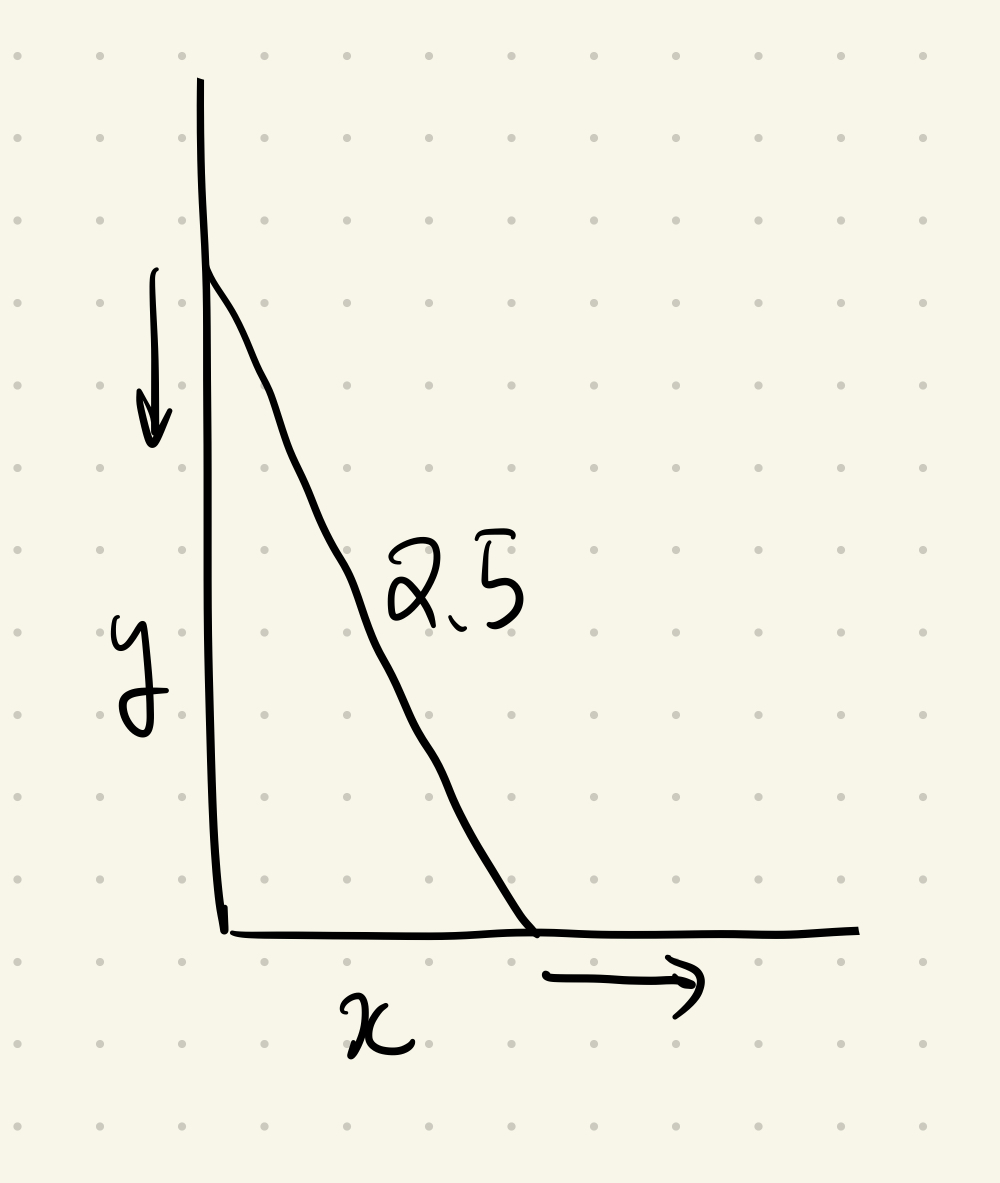
\includegraphics[width = 0.3\textwidth, trim={0 2cm 0 3cm}, clip]{figures/chap 05/rel_rates_ladder.png}
        \label{fig: rel_rates_ladder}    
    \end{center}
    where $x$ (in meters) is the distance between the ladder foot and the wall base, and $y$ (in meters) is the height of the ladder tip.  From Pythagorean theorem, we relate $x$ and $y$ by:
    \[x^2+y^2 = 2.5^2 = 6.25\]
    To obtain the related rates between $x$ and $y$, we differentiate both sides by $t$ (denoting $()'$ as differentiation with respect to $t$):
    \begin{align*}
        (x^2+y^2)' &= (6.25)'\\
        2xx'+2yy' &= 0\\
        y' &= -\frac{xx'}{y}  \quad  (\because y > 0)
    \end{align*}
    Since the foot of the ladder is moving \textit{away} from the wall with speed $0.2$m/sec, and it is currently $1.5$m away from the wall base, we have
    \[x' = 0.2 \qquad x = 1.5 \qquad y = \sqrt{2.5^2-1.5^2} = 2\]
    Therefore, 
    \[y' = -\frac{0.2 \cdot 1.5}{2} = -0.15\]
    So the tip of the ladder is sliding down with speed $15$cm/s. (The negative sign in $y'$ indicates that $y$ is decreasing, which reflects that the tip is sliding down.)
\end{egsol}

\begin{ex}[]{ex: related_rates_orbit}
    \begin{center}
        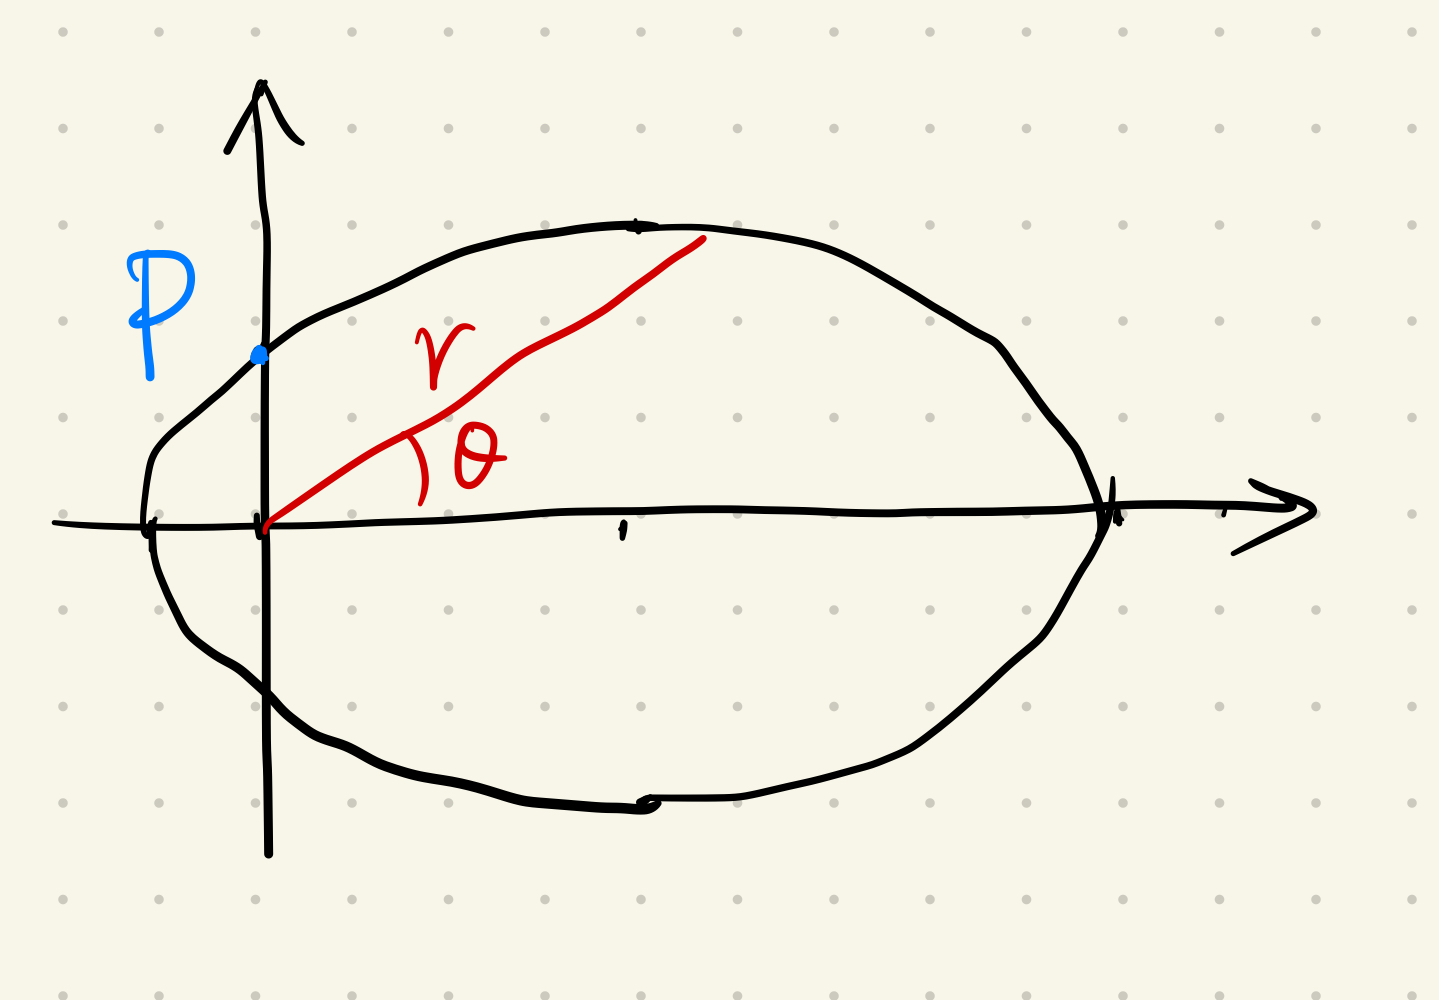
\includegraphics[width = 0.3\textwidth]{figures/chap 05/rel_rates_orbit.png}
        \label{fig: rel_rates_orbit}    
    \end{center}
    Shown in the figure above, a moon is orbiting counter-clockwise around a planet at the origin point.  The orbit, which is an ellipse, can be described as follows:
    %\[\frac{(r\cos \theta - 4)^2}{25} + \frac{(r \sin \theta)^2}{9} = 1\]
    \[r\Big(1-\frac{4}{5}\cos \theta \Big) = \frac{9}{5}\]
    where $r$ (in AU, astronomical unit) is the distance between the moon and the planet, and $\theta$ is the directed angle from the long axis of the ellipsis to the moon-planet line.  Suppose an astronomer observed that the angular velocity of the moon at point $P$ is $0.2$ radians/day, how fast is the moon-planet distance decreasing at that time?
\end{ex}

\begin{exsol}[]{exsol: related_rates_orbit}

    We try to find the related rate by differentiating both sides of the orbit equation by time $t$ (in days).  For brevity, we denote $()'$ as differentiation with respect to $t$:
    \begin{align*}
        % \left[\frac{(r\cos \theta - 4)^2}{25} + \frac{(r \sin \theta)^2}{9}\right]' &= (1)' = 0\\
        % \frac{\big[(r \cos \theta - 4)^2\big]'}{25} + \frac{\big[(r \sin \theta)^2\big]'}{9}&= 0\\
        % \frac{\big[(r \cos \theta - 4)^2\big]'}{25} &= -\frac{\big[(r \sin \theta)^2\big]'}{9}\\
        % \frac{2(r\cos \theta -4)(r\cos \theta -4)'}{25} &= - \frac{2(r\sin \theta) (r\sin\theta)'}{9}\\
        % \frac{(r\cos \theta -4)(r'\cos \theta -r(\sin \theta)\theta' )}{25} &= - \frac{(r\sin \theta) (r'\sin\theta + r (\cos \theta) \theta')}{9}
        \Big[r\Big(1-\frac{4}{5}\cos \theta \Big)\Big]' &= \Big(\frac{9}{5}\Big)'\\
        r'\Big(1-\frac{4}{5}\cos \theta \Big) + r\Big(1-\frac{4}{5}\cos \theta \Big)'&= 0\\
        r'\Big(1-\frac{4}{5}\cos \theta \Big) + r\Big(-\frac{4}{5} (-\sin \theta) \theta')'&= 0\\
        r'\Big(1-\frac{4}{5}\cos \theta \Big) + \frac{4}{5} r \theta' \sin \theta &= 0
    \end{align*}
    At point $P$, we have $\theta = \frac{\pi}{2}$ and $\theta' = 0.2$.  Plugging in $\theta = \frac{\pi}{2}$ into the orbit equation and we can solve for $r$ at point $P$:
    \[r = \frac{9}{5}\Big/\Big(1-\frac{4}{5}\cos \frac{\pi}{2} \Big) = \frac{9}{5}\]
    %\begin{align*}
        % \frac{(r\cos \frac{\pi}{2} - 4)^2}{25} + \frac{(r \sin \frac{\pi}{2})^2}{9} &= 1\\
        % \frac{16}{25} + \frac{r^2}{9} &= 1\\
        % r^2 &= \frac{81}{25}  \Rightarrow r = \frac{9}{5} \quad (\because r \ge 0)
    %\end{align*}
    We can then plug in $\theta = \frac{\pi}{2}$, $\theta' = 0.2$ and $r = \frac{9}{5}$ into the previous equation and yield
    \begin{align*}
        r'\Big(1-\frac{4}{5}\cos \frac{\pi}{2} \Big) + \frac{4}{5} \frac{9}{5} \cdot 0.2 \cdot \sin \frac{\pi}{2} &= 0\\
        r' + \frac{36}{125} &= 0 \quad \Rightarrow \quad r' = -\frac{36}{125} = -0.288
    \end{align*}
    Therefore, the moon-planet distance is decreasing at a rate of $0.288$ AU/day, where the negative sign we've got indicates that the distance is decreasing.
\end{exsol}

\begin{ex}[]{ex: related_rates_cars}
    Two cars $A$ and $B$ are driving away from town $O$. $A$ is driving straight to the east, while $B$ is driving toward the north-east, so that the routes of the two cars are $45\degree$ apart.  Suppose $A$ is $20$ km from town $O$ and driving at $60$ km/hr, and $B$ is $20\sqrt{2}$ km from town $O$ and driving at $100$ km/hr.  What is the rate of change for the distance between the two cars?
\end{ex}

\begin{exsol}[]{egsol: related_rates_car}
    Let the distance between $A$ and $O$ be $a$ (kilometers), between $B$ and $O$ be $b$ (kilometers), and distance between $A$ and $B$ be $c$ (kilometers).  From the Cosine Theorem, we have the relationship between $a$, $b$ and $c$ as:
    \[c^2 = a^2 + b^2 - 2ab\cos 45 \degree = a^2 + b^2 - \sqrt{2}ab\]
    We try to find the related rate by differentiating both sides by time $t$ (in seconds).  For brevity, we denote $()'$ as differentiation with respect to $t$:
    \begin{align*}
        (c^2)' &= (a^2 + b^2 - \sqrt{2}ab)'\\
        2cc' &= 2aa' + 2bb' - \sqrt{2}(ab)'\\
        2cc' &= 2aa' + 2bb' - \sqrt{2}a'b - \sqrt{2}ab'\\
        c' &= \frac{aa' + bb' - \frac{1}{\sqrt{2}}a'b - \frac{1}{\sqrt{2}}ab'}{c} \quad (\text{if } c \ne 0)
    \end{align*}
    The current distance between the two cars (i.e., $c$) can also be found by the Cosine Theorem, which is
    \[c = \sqrt{20^2+(20\sqrt{2})^2-2 \cdot 20 \cdot 20\sqrt{2} \cdot \frac{1}{\sqrt{2}}} = \sqrt{400+800-800} = \sqrt{400} = 20\]
    Therefore, we can then plug in $a = 20$, $a' = 60$, $b = 20\sqrt{2}$, $b' = 100$ and $c = 20$ into the previous equation and yield
    \[c' = \frac{20 \cdot 60 + 20\sqrt{2} \cdot 100 - \frac{1}{\sqrt{2}}\cdot 60\cdot 20\sqrt{2} - \frac{1}{\sqrt{2}} \cdot 20 \cdot 100}{20} = 50\sqrt{2}\]
    Therefore, the distance between the two cars is increasing at the speed of $50\sqrt{2}$ km/hr.
\end{exsol}

\pagebreak
\section{Curve Sketching}
At times you would want to know the behavior a function by graphing it on a Cartesian plane.  However, you would want the graph to be as informative as possible.  For example, for $f(x) = 4x - \frac{1}{2}x^2$, the graph on the left below is very accurate in the region it is plotting, and the graph on the right is a little bit distorted in scale.  However, the one on the right captures important features of the function (i.e. the vertex of the parabola, where it's facing, its $x$-intercepts). Therefore, it is preferred since it carries way more information.

\begin{figure}[ht]
    \centering
    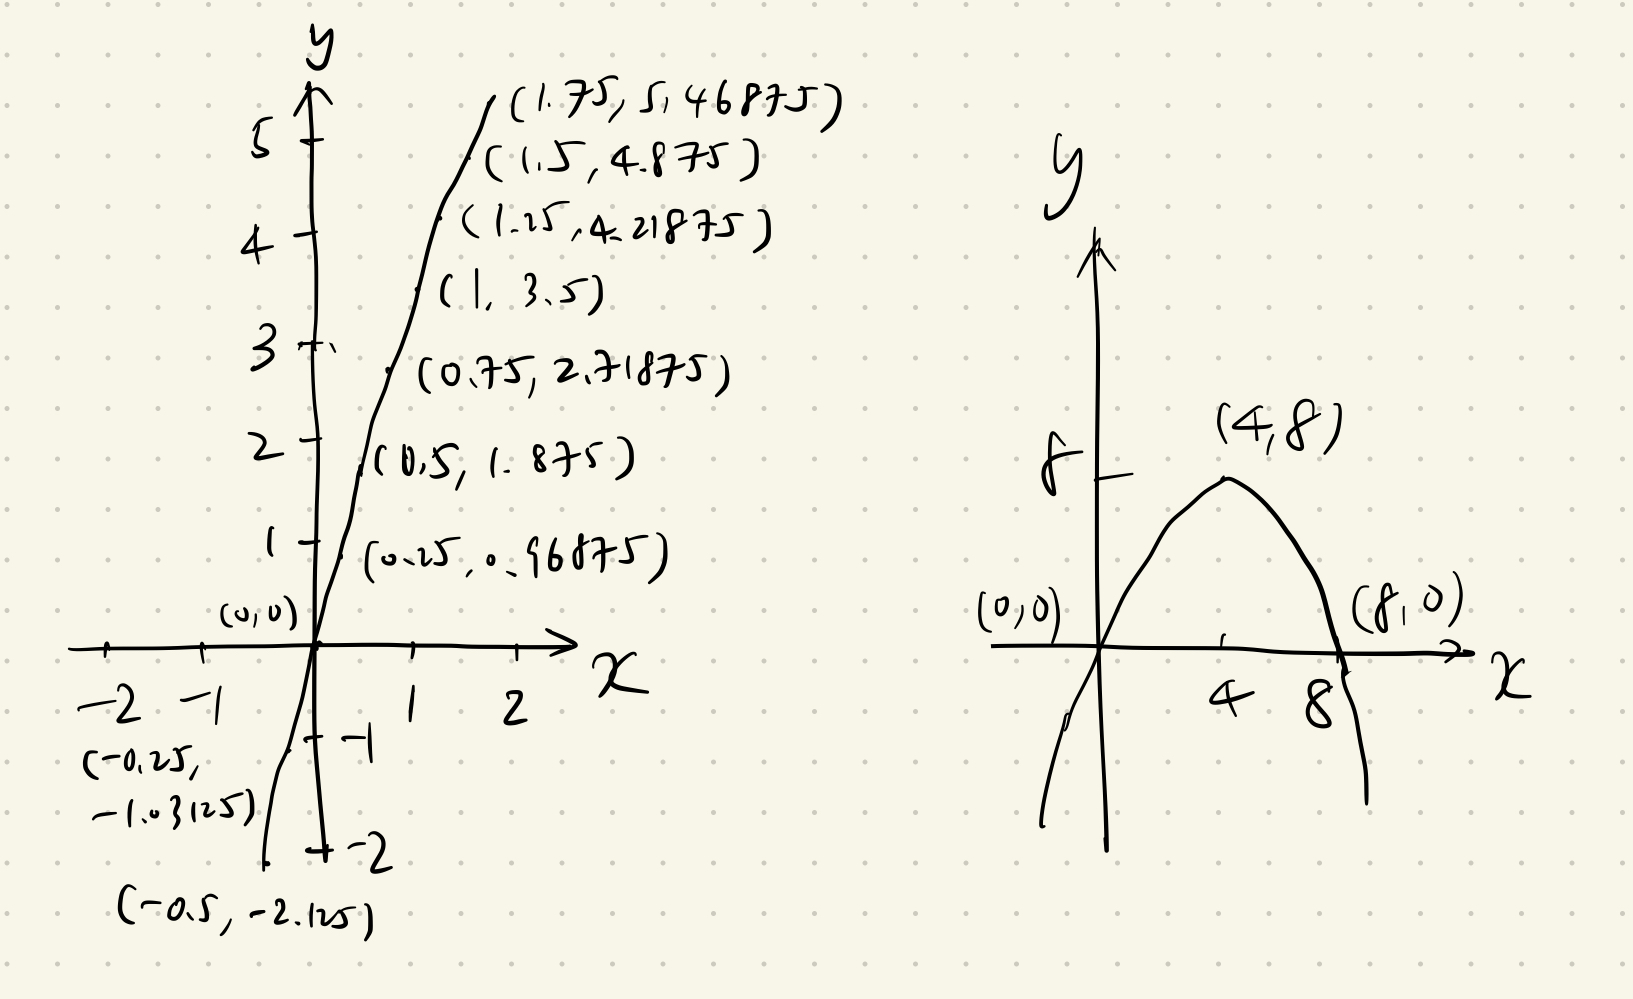
\includegraphics[width = 0.75\textwidth]{figures/chap 05/sketching_demo.png}
    \label{fig: sketching_demo}
\end{figure}

Up until now, we have already known how to tap into several features of a function $f(x)$, including:
\begin{itemize}
    \item Discontinuities and behavior at discontinuities: Find values $c$ where $f(c)$ is undefined, or where $\lim_{x\rightarrow c}f(x) \ne f(c)$. The latter usually happens when $f(x)$ is piecewise defined.  We can then try to evaluate $f(c)$, $\lim_{x \rightarrow c^+}f(x)$ and $\lim_{x \rightarrow c^-}f(x)$ to ascertain the behavior of $f(x)$ around and at $x=c$.
    \item Behavior at boundaries: We may evaluate the behavior of the function at its domain boundaries by taking its limit at that boundary. For example, if the domain of $f$ is $(\ell, u)$, then we can try to evaluate $\lim_{x \rightarrow \ell^+}f(x)$ and $\lim_{x \rightarrow u^-}f(x)$ and see if the function converge to a value, or blows up to $\pm \infty$.  Alternatively, if the domain is unbounded (eg. $\mathbb{R}$), we can try finding $\lim_{x \rightarrow \infty}f(x)$ and $\lim_{x \rightarrow -\infty}f(x)$.
    \item $y$-intercept: Plug $0$ into $x$.
    \item $x$-intercepts (roots): Let $f(x)=0$ and solve for $x$.
\end{itemize}

Apart from the features above (which you \textit{should} include in your curve sketching if possible), as we will soon see, the behavior of the function is also largely governed by its first derivative $f'$ and second derivative $f''$.  Therefore, a big part of curve sketching is to determine where $f'$ and $f''$ are zero, positive or negative.  We will first start with the first derivative $f'$.

\subsection{First Derivative and Critical Points}

Given a function $f$, its first derivative $f'$ governs if $f$ is \textit{increasing} or \textit{decreasing}.  The concept of (strictly) increasing and decreasing is straightforward: if $f(x)$ is getting larger as $x$ is getting larger, then $f(x)$ is increasing, vice versa.  The reason why we added "(strictly)" is that by convention in mathematics, "increasing" and "decreasing" permits the possibility where $f(x)$ remains the same value as $x$ is getting larger.  This can be illustrated by the following graphs:

\begin{figure}[ht]
    \centering
    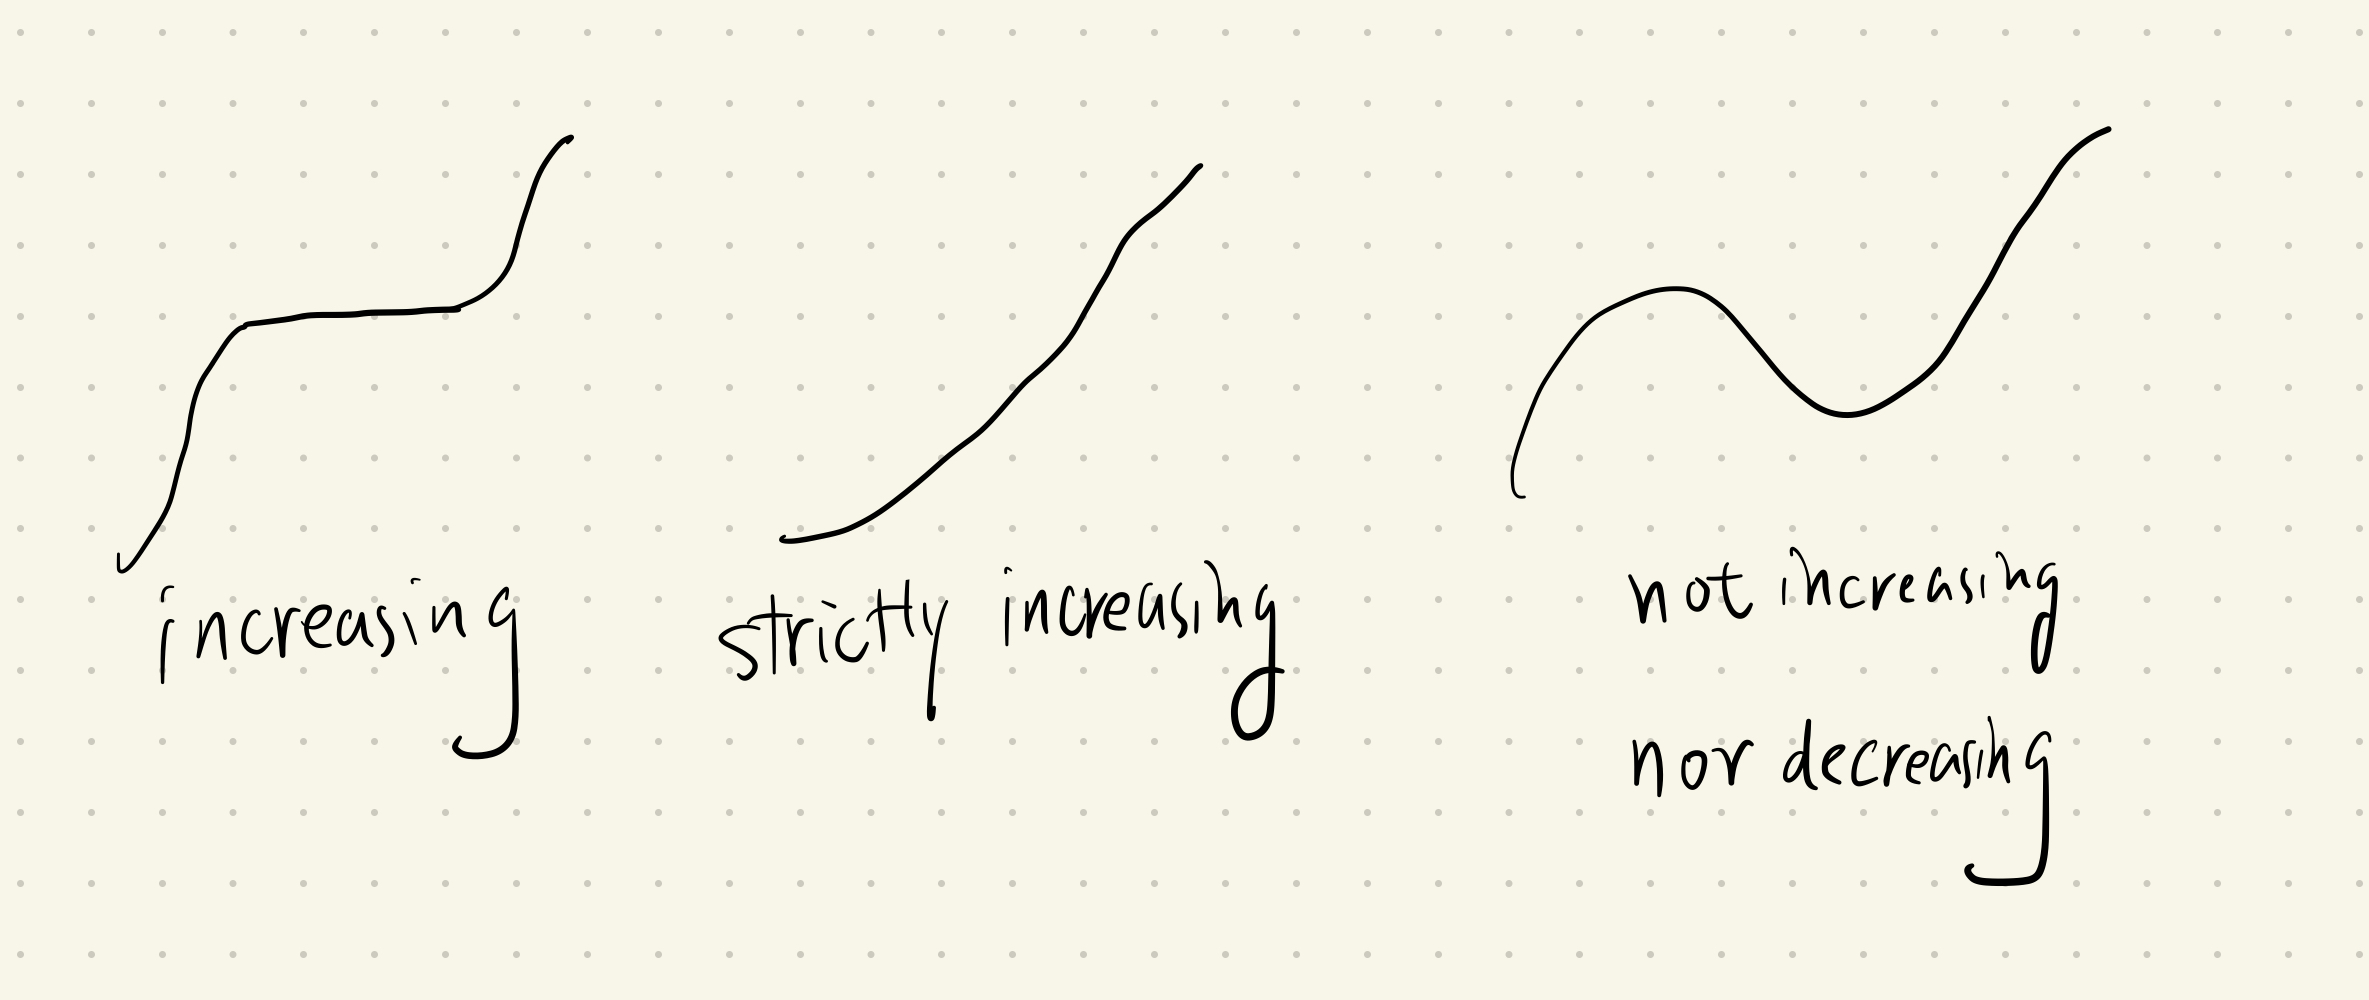
\includegraphics[width = 0.8\textwidth]{figures/chap 05/def_increasing_decreasing.png}
    \label{fig: def_increasing_decreasing}
\end{figure}

We hereby include the formal definition of increasing and decreasing functions for completeness:

\begin{defi}[Increasing and decreasing functions]{def: increasing_decreasing}
    Let $I$ be an interval and $x_1, x_2$ be any two numbers in $I$. A function $f(x)$ is:
    \begin{itemize}
        \item \textit{increasing} in $I$ if $x_1 > x_2$ implies $f(x_1) \ge f(x_2)$.
        \item \textit{strictly increasing} in $I$ if $x_1 > x_2$ implies $f(x_1) > f(x_2)$.
        \vspace{0.5cm}
        \item \textit{decreasing} in $I$ if $x_1 > x_2$ implies $f(x_1) \le f(x_2)$.
        \item \textit{strictly decreasing} in $I$ if $x_1 > x_2$ implies $f(x_1) < f(x_2)$.
    \end{itemize}
\end{defi}

To relate the derivative of a function to whether it is strictly increasing or decreasing, we can look at the following graph:
\begin{enumerate}
    \item In the left panel, the slope of the tangent lines (i.e. the derivatives) are always \textit{positive} within $(a, b)$, and we see that the function is \textit{strictly increasing} in $(a, b)$.
    \item In the right panel, the slopes of the tangent lines are always \textit{negative} within $(a, b)$, and the function is \textit{strictly decreasing} in $(a, b)$.  
\end{enumerate}
 
\pagebreak

\begin{figure}[ht]
    \centering
    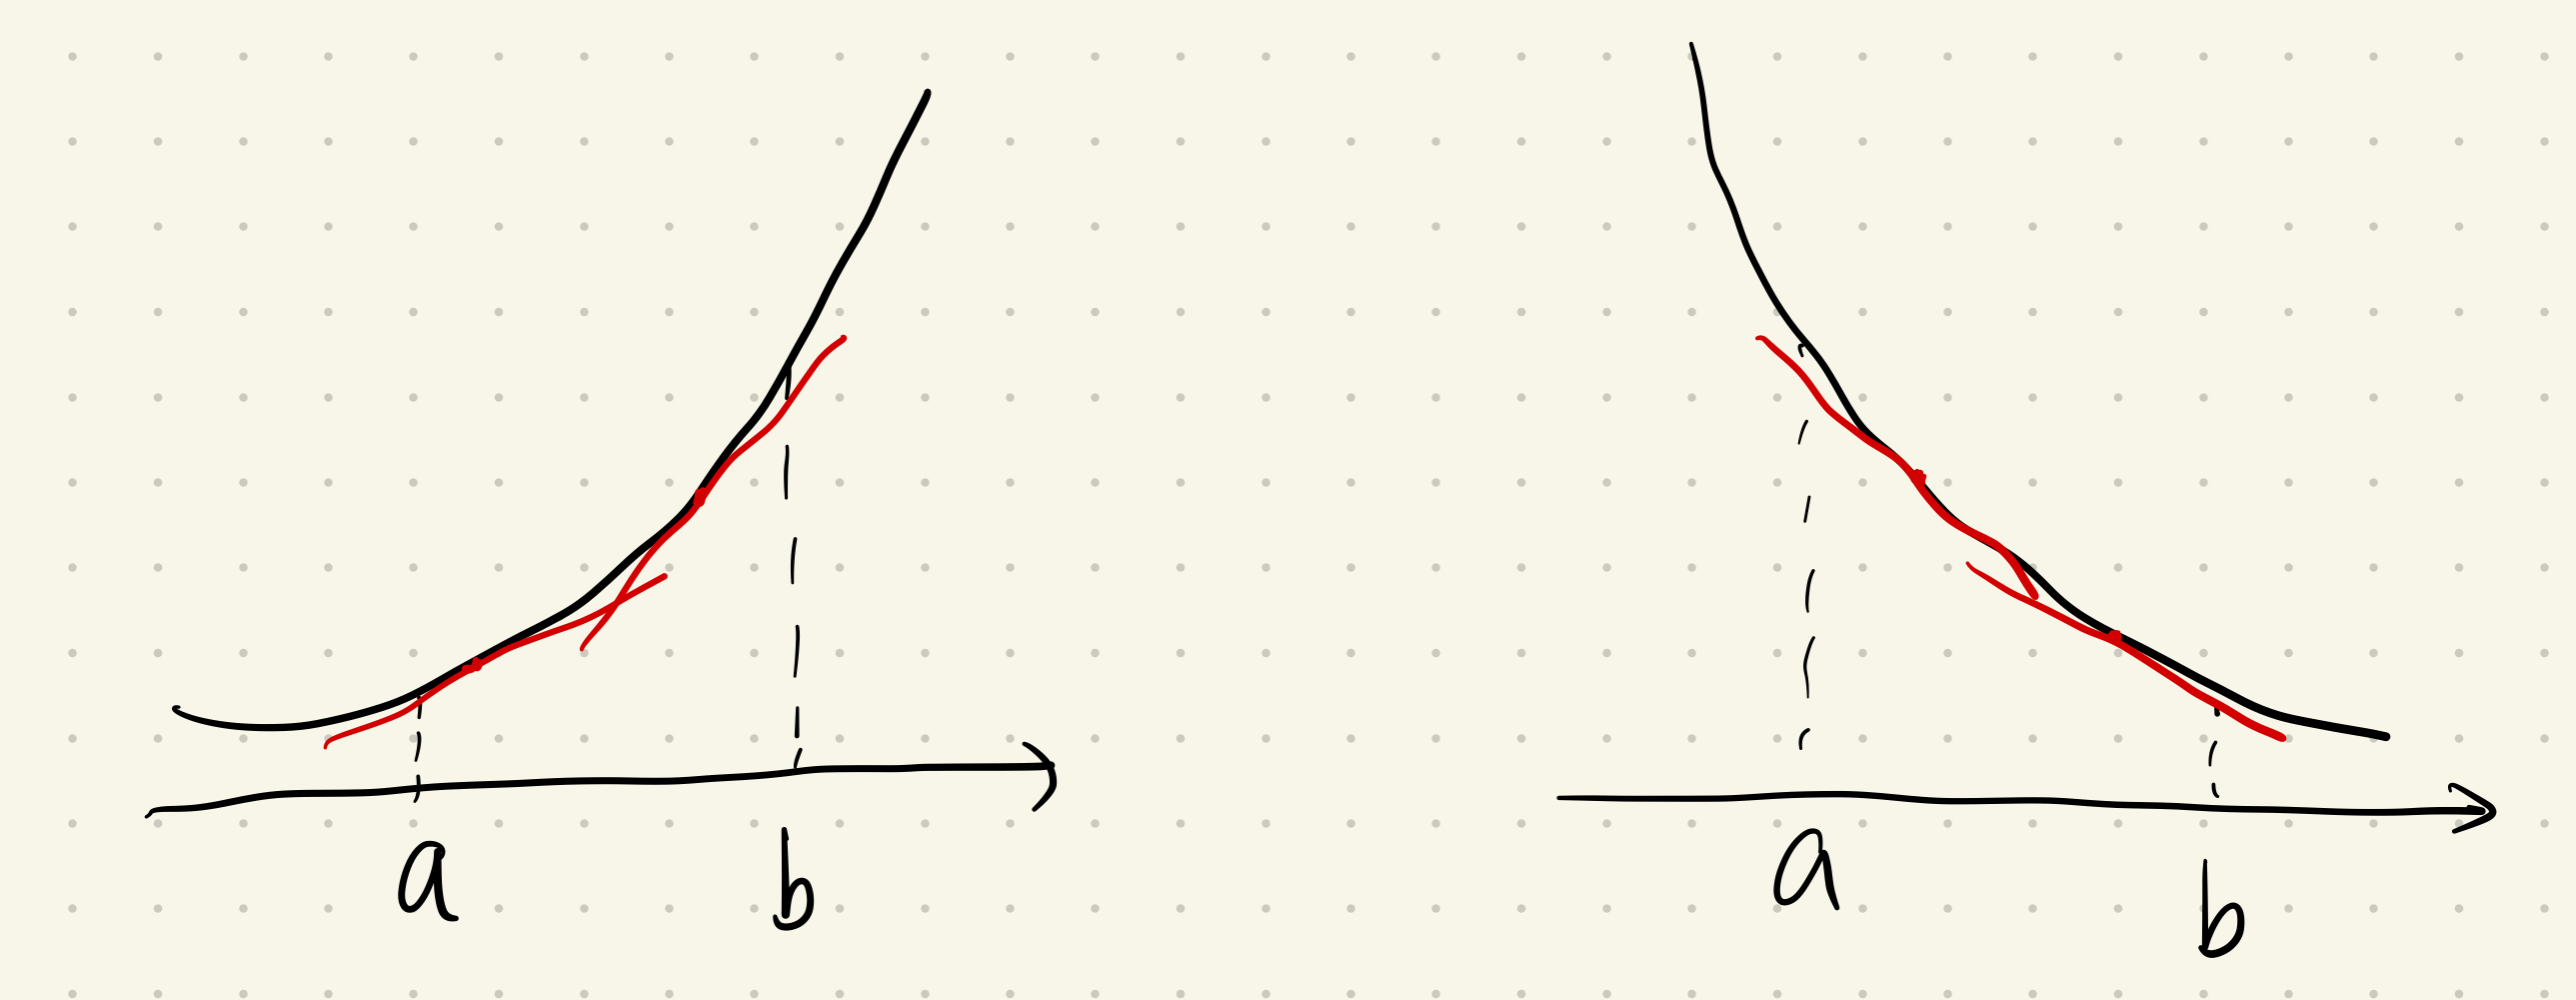
\includegraphics[width = 0.7\textwidth]{figures/chap 05/increasing_decreasing.png}
    \label{fig: increasing_decreasing}
\end{figure}

We can summarize our findings into the following theorem:

\begin{theo}[Derivative and strict monotonicity]{thm: derivative_to_monotone}
    Suppose a function $f(x)$ is differentiable in $(a, b)$, then:
    \[f'(x) > 0, \forall x \in (a, b) \Rightarrow f(x) \text{ is \textit{strictly increasing} in } (a,b)\]
    \[f'(x) < 0, \forall x \in (a, b) \Rightarrow f(x) \text{ is \textit{strictly decreasing} in } (a,b)\]
    If in addition $f(x)$ is continuous in $[a, b]$, then
    \[f'(x) > 0, \forall x \in (a, b) \Rightarrow f(x) \text{ is \textit{strictly increasing} in } [a,b]\]
    \[f'(x) < 0, \forall x \in (a, b) \Rightarrow f(x) \text{ is \textit{strictly decreasing} in } [a,b]\]
\end{theo}

We will prove this theorem rigorously in later subsections, and now we will focus on its practical use.  For a function $f(x)$, we may try to find intervals for $x$ where $f'(x)$ is positive, so we would know that $f(x)$ is strictly increasing in this region.  Likewise, we may find intervals where $f'(x)$ is negative so that $f(x)$ is strictly decreasing in that region.  This can be demonstrated with the following example:

\begin{eg}[]{eg: increasing_decreasing}
    Find intervals on which the function $f(x) = x^5 + 5x^4 - 20x^3 + 30$ is increasing or decreasing.
\end{eg}

\begin{egsol}[]{egsol: increasing_decreasing}
    We first calculate the derivative of $f(x)$, which is
    \[f'(x) = 5x^4 + 20x^3 - 60x^2 = 5x^2(x^2+4x-12) = 5x^2(x-2)(x+6)\]
    To find where $f'(x)$ is positive or negative, we can first determine where $f'(x) = 0$, i.e. find the roots for $f'(x)$.  These roots can then serve as anchor points to help us find regions where $f'(x)$ is positive or negative.
    
    Since $f'(x)$ has three distinct roots $0, 2, -6$, we can divide the number line into four regions with these three roots: $(-\infty, -6)$, $(-6, 0)$, $(0, 2)$ and $(2, \infty)$, illustrated in the graph below: 
    \begin{center}
        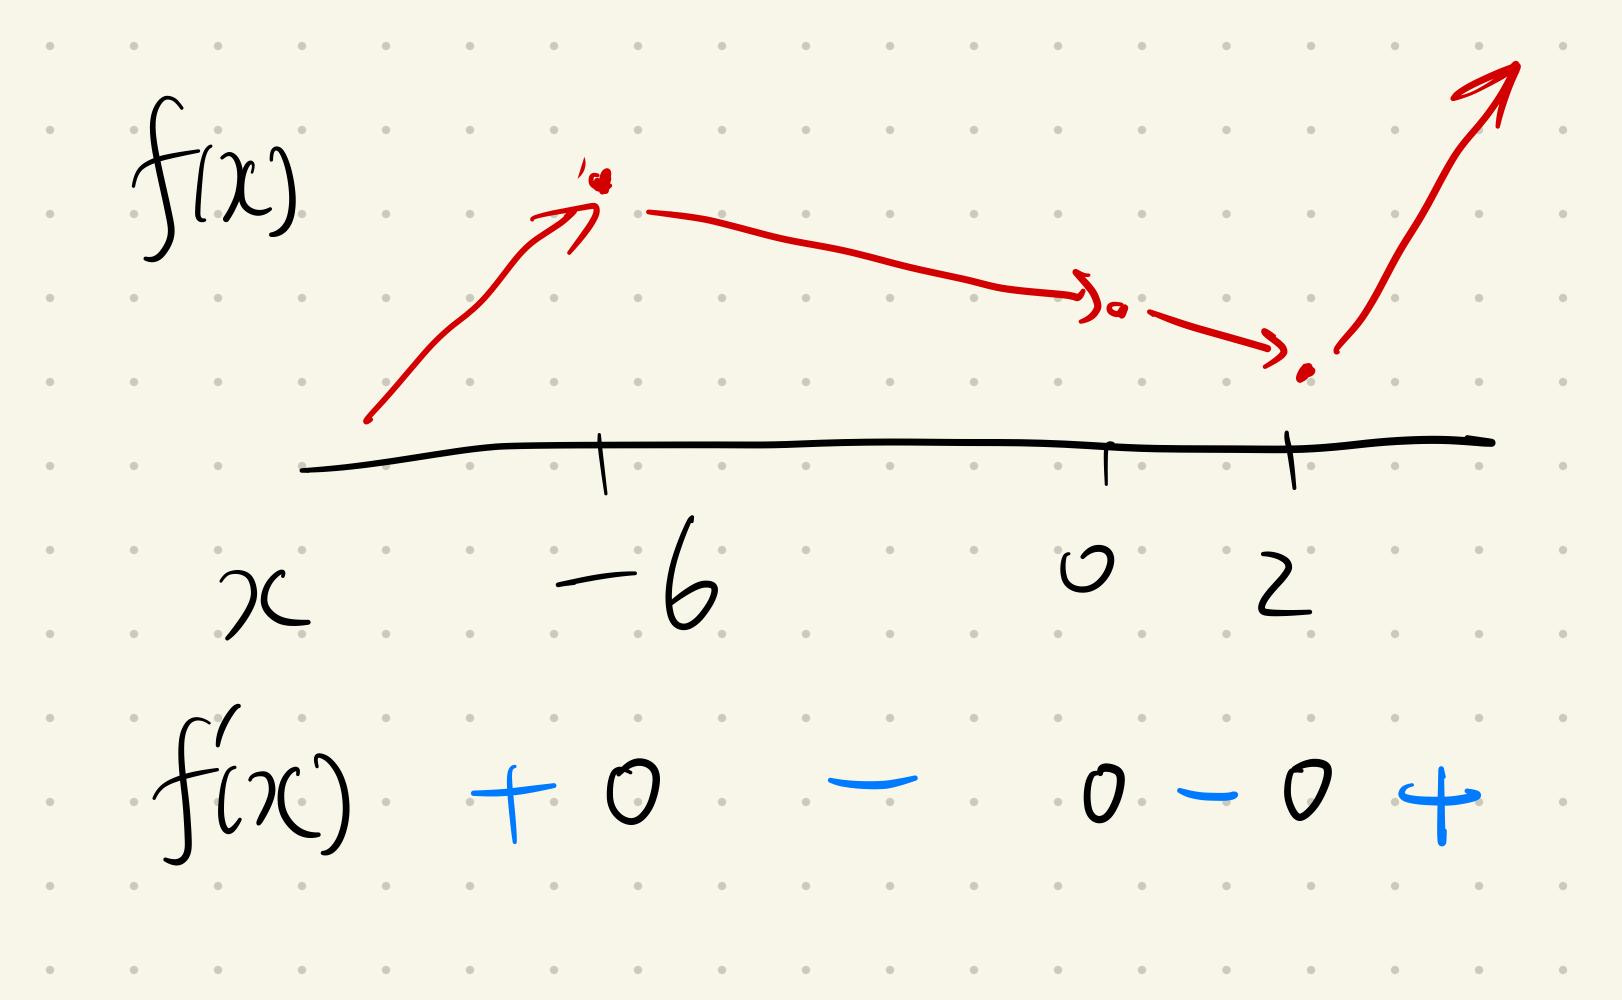
\includegraphics[width = 0.5\textwidth]{figures/chap 05/eg_increasing_decreasing.png}
        \label{fig: eg_increasing_decreasing}
    \end{center}
    We now assess the sign of $f'(x) = 5 (x+6) \cdot x \cdot x \cdot (x-2)$ in each interval by evaluating the sign of each factor, i.e. $x+6$, $x$, $x$ and $x-2$:
    \begin{itemize}
        \item $(2, \infty):$ All factors of $f'(x)$ are positive in this interval, so $f'(x)$ is positive.
        \item $(0, 2):$ We have three positive factors ($x+6$, $x$, $x$) and one negative factor ($x-2$), so $f'(x)$ is negative.
        \item $(-6, 0):$ We have one positive factor ($x+6$) and three negative factors ($x$, $x$, $x-2$), so $f'(x)$ is negative.
        \item $(-\infty, -6):$ We have all four factors negative, so $f'(x)$ is positive.
    \end{itemize}
    From Theorem~\ref{thm: derivative_to_monotone}, since $f(x)$ is a polynomial and thus differentiable and continuous in $\mathbb{R}$, it is strictly increasing in $(-\infty, -6]$ and $[2, \infty)$ and strictly decreasing in $[-6, 2]$.  We can then sketch the increasing and decreasing behavior of $f(x)$ based on our finding, also shown in the graph.
\end{egsol}

\begin{remark}
    From the graph we can see that as $x$ is increasing from the left side of the number line, $f(x)$ is increasing until $x = -6$, then it decreases until $x = 2$, then it increases again.  Therefore, $f(-6)$ and $f(2)$ are the "local maximum" and "local minimum" of the function, i.e. $f(x)$ has a peak at $x = -6$ and a valley at $x = 2$.  We will talk more about this later when we are using derivatives to obtain extrema. 
\end{remark}

\begin{remark}
    In this example, we first identified points where $f'(x) = 0$ to aid us finding intervals where $f(x)$ is increasing and decreasing.  In fact, points where $f'(x) = 0$ or $f'(x)$ is undefined carry a great deal of information on the behavior of $f(x)$, and they deserve a dedicated name defined below:
\end{remark}

\begin{defi}[Critical points and critical values]{def: crit}
    A point $x=c$ in the domain of $f(x)$ is termed as a \textit{critical point} for $f(x)$ if $f'(c) = 0$ or $f'(c)$ does not exist.  The function value $f(c)$ is then termed as a \textit{critical value} for $f(x)$ associated with the critical point $x=c$.
\end{defi}

The reason why we care about critical points is that the behavior of a function near its critical points is often interesting.  Therefore, knowing where the critical points are helps us know the function better.  For example, lets take a look at the following graph showing seven critical points of a function:

\begin{figure}[ht]
    \centering
    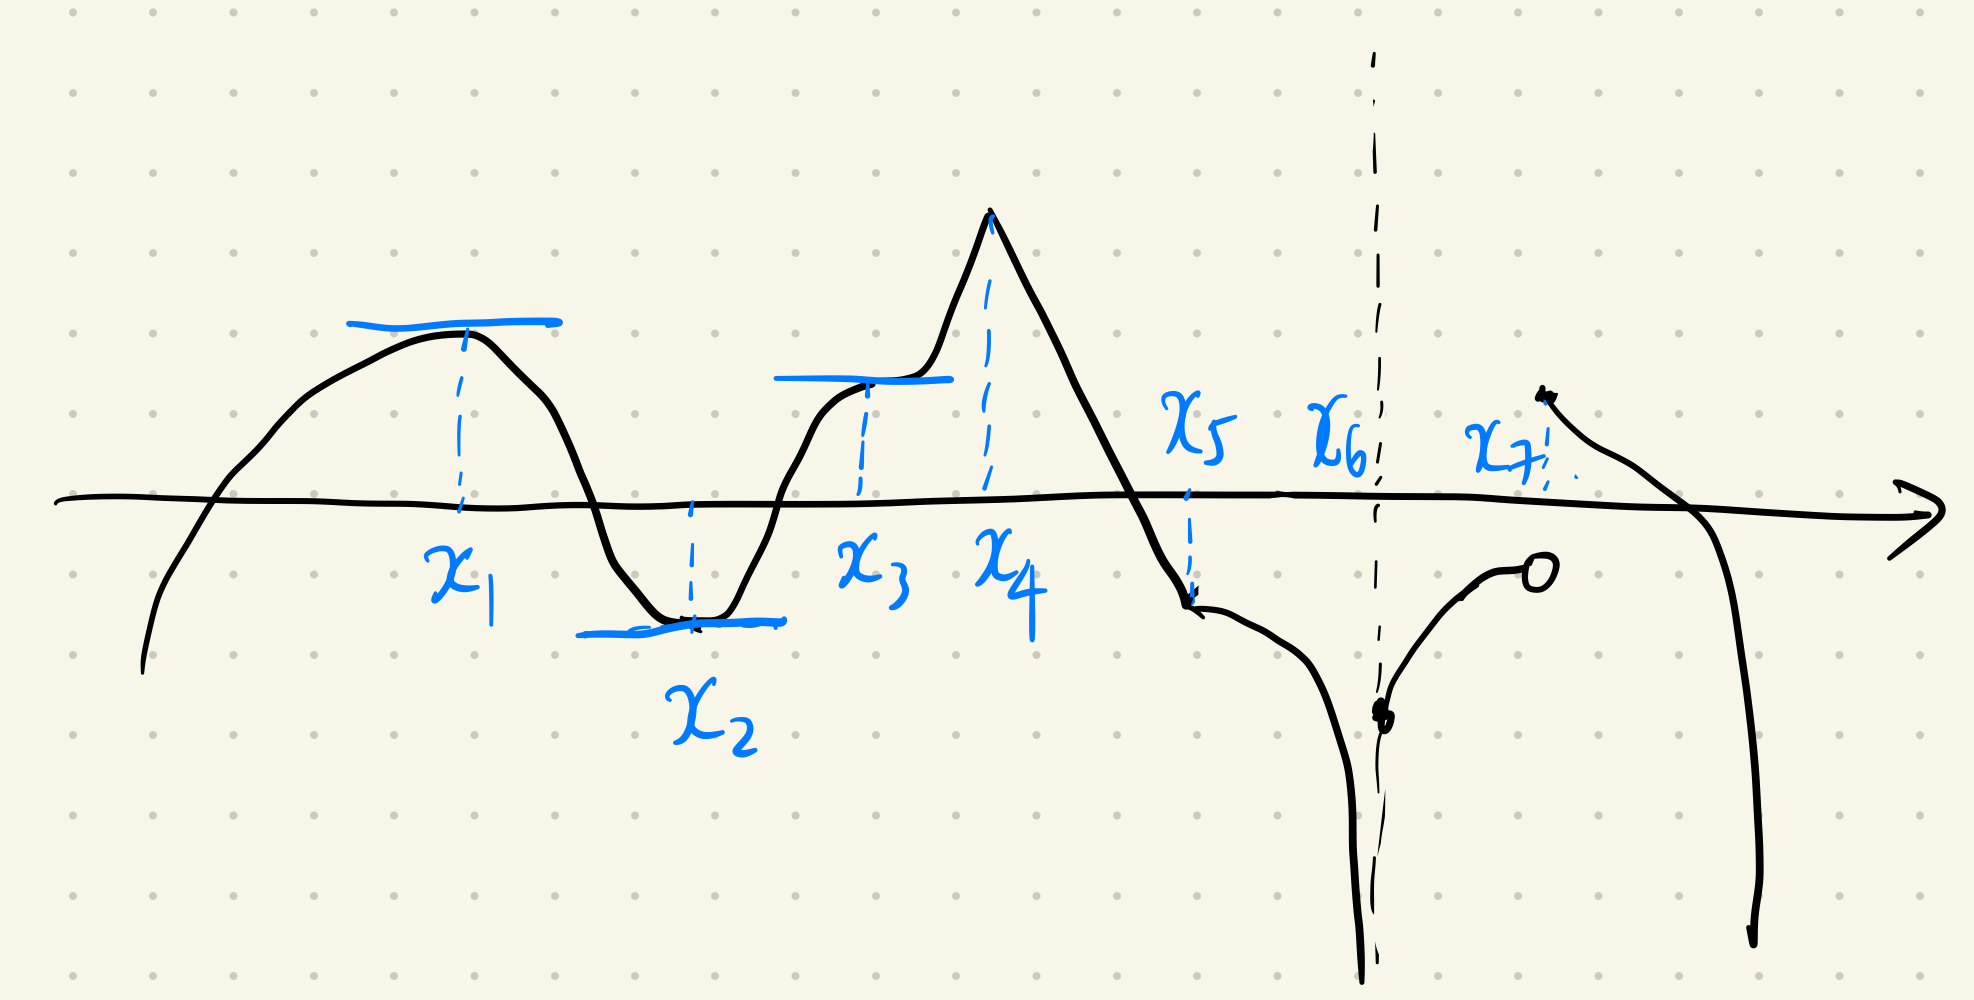
\includegraphics[width = 0.75\textwidth]{figures/chap 05/critical_points.png}
    \label{fig: critical_points}
\end{figure}

The points $x = x_1$ and $x = x_2$ are both critical points since $f'(x_1) = f'(x_2) = 0$.  These points are special since \textit{local maximum} is attained at $x = x_1$ and \textit{local minimum} is attained at $x = x_2$.

The point $x = x_3$ is also a critical point since $f'(x_3) = 0$.  This time, $x=x_3$ does not lead to local maximum or minimum, but it is an \textit{inflection point}, where the curve is turning from a bowl facing down (concave down) to a bowl facing up (concave up).  We will talk about this more when we get to second derivatives.

The points $x = x_4$ and $x = x_5$ are both critical points since $f'(x_4)$ and $f'(x_5)$ both do not exist due to a \textit{kink} in the curve.  Sometimes a local maximum and minimum will also occur at these points.  In this case, local maximum is attain at $x = x_4$.

The points $x = x_6$ and $x = x_7$ are also critical points since $f'(x_6)$ and $f'(x_7)$ both do not exist due to \textit{discontinuity}.  Finding these discontinuities will alert us that the function either has a jump or goes to $\pm\infty$, leading to better curve sketching.  Local maximum or minimum can still occur at these discontinuities, such as $x = x_7$.

With the additional information of critical points and first derivatives, we can form a procedure to sketch a function $f$ (without using second derivatives for now):

\begin{enumerate}
    \item \textit{Domain and behavior at boundaries}: Assess the behavior of $f$ at the boundary of its domain.
    \item \textit{Find discontinuities}: Find all discontinuities in $f$.
    \item \textit{Behavior at discontinuities}: Assess the behavior of $f$ at the discontinuities ($f(c)$ and the left / right limits of $f(c)$ at $x=c$).
    \item \textit{Find and plot critical points}: Find the critical points / values of $f$ (this may include some discontinuities we've found in the first step) and plot them.
    \item \textit{Behavior between critical points / discontinuities}: Assess if the function is increasing or decreasing between the critical points and discontinuities using the sign of $f'$.
    \item \textit{Miscellaneous}: (Optional) Plot "easy points" of $f$, eg. the $x$- and $y$- intercepts.
\end{enumerate}

Connecting all features in the procedure would lead to the final sketch. We now illustrate this procedure with a couple of examples.

\begin{eg}[]{eg: first_derivative}
    Find the critical points for $f(x) = \frac{2x-1}{x+1}$ and sketch $f(x)$ using the information of its first derivative.
\end{eg}

\begin{egsol}[]{egsol: first_derivative}
    To find the critical points for $f(x)$, we first find its first derivative:
    \[f'(x) = \frac{2 \cdot (x+1)-(2x-1) \cdot 1}{(x+1)^2} = \frac{3}{(x+1)^2}\]
    Therefore, $f'(x)$ is always positive except for $x = -1$ where it's undefined.  However, $x = -1$ is not in the domain of $f(x)$, so there are no critical points for $f(x)$.
    
    To sketch $f(x)$, we follow the steps of the procedure mentioned above:
    
    \begin{enumerate}
        \item \textit{Domain and behavior at boundaries}: The domain of $f(x)$ is $\mathbb{R} \backslash \{-1\}$, so we assess its limit at $\pm\infty$.  Since $f(x)$ is a rational function with polynomials of the same degree ($1$) at the numerator and denominator, we have
        \[\lim_{x \rightarrow \infty} f(x) = \lim_{x \rightarrow -\infty} f(x) = \frac{2}{1} = 2\]
        Therefore, $f(x)$ has a horizontal asymptote at $y = 2$ for both the left and right sides of the graph.
        \item \textit{Find discontinuities}: The only discontinuity in $f(x)$ is where its denominator equals zero, i.e. $x = -1$.
        \item \textit{Behavior at discontinuities}: $f(x)$ is undefined at $x=-1$.  The right-side limit at $x=-1$ is 
        \[\lim_{x \rightarrow (-1)^+} \frac{2x-1}{x+1} = \frac{-3}{0^+} = -\infty\]  
        While the left-side limit is
        \[\lim_{x \rightarrow (-1)^-} \frac{2x-1}{x+1} = \frac{-3}{0^-} = \infty\]
        Therefore, $f(x)$ has a vertical asymptote at $x = -1$, with its value shooting down to $-\infty$ on the right and up to $\infty$ on the left.
        \item \textit{Find and plot critical points}: We have shown that there are no critical points for $f(x)$
        \item \textit{Behavior between critical points / discontinuities}: We now determine the sign of $f'(x) = \frac{3}{(x+1)^2}$ in $(-\infty, 1)$ and $(1, \infty)$, which should both be positive.  Therefore, $f(x)$ is strictly increasing in both $(-\infty, 1)$ and $(1, \infty)$.
        \item \textit{Miscellaneous}: It is easy to find the $x$- and $y$-intercepts of $y=f(x)$, which are $\big(\frac{1}{2}, 0\big)$ and $(0, -1)$.  We can plot them on the graph.
    \end{enumerate}
    
    Combining the information above would lead us to the graph below:
    \begin{center}
        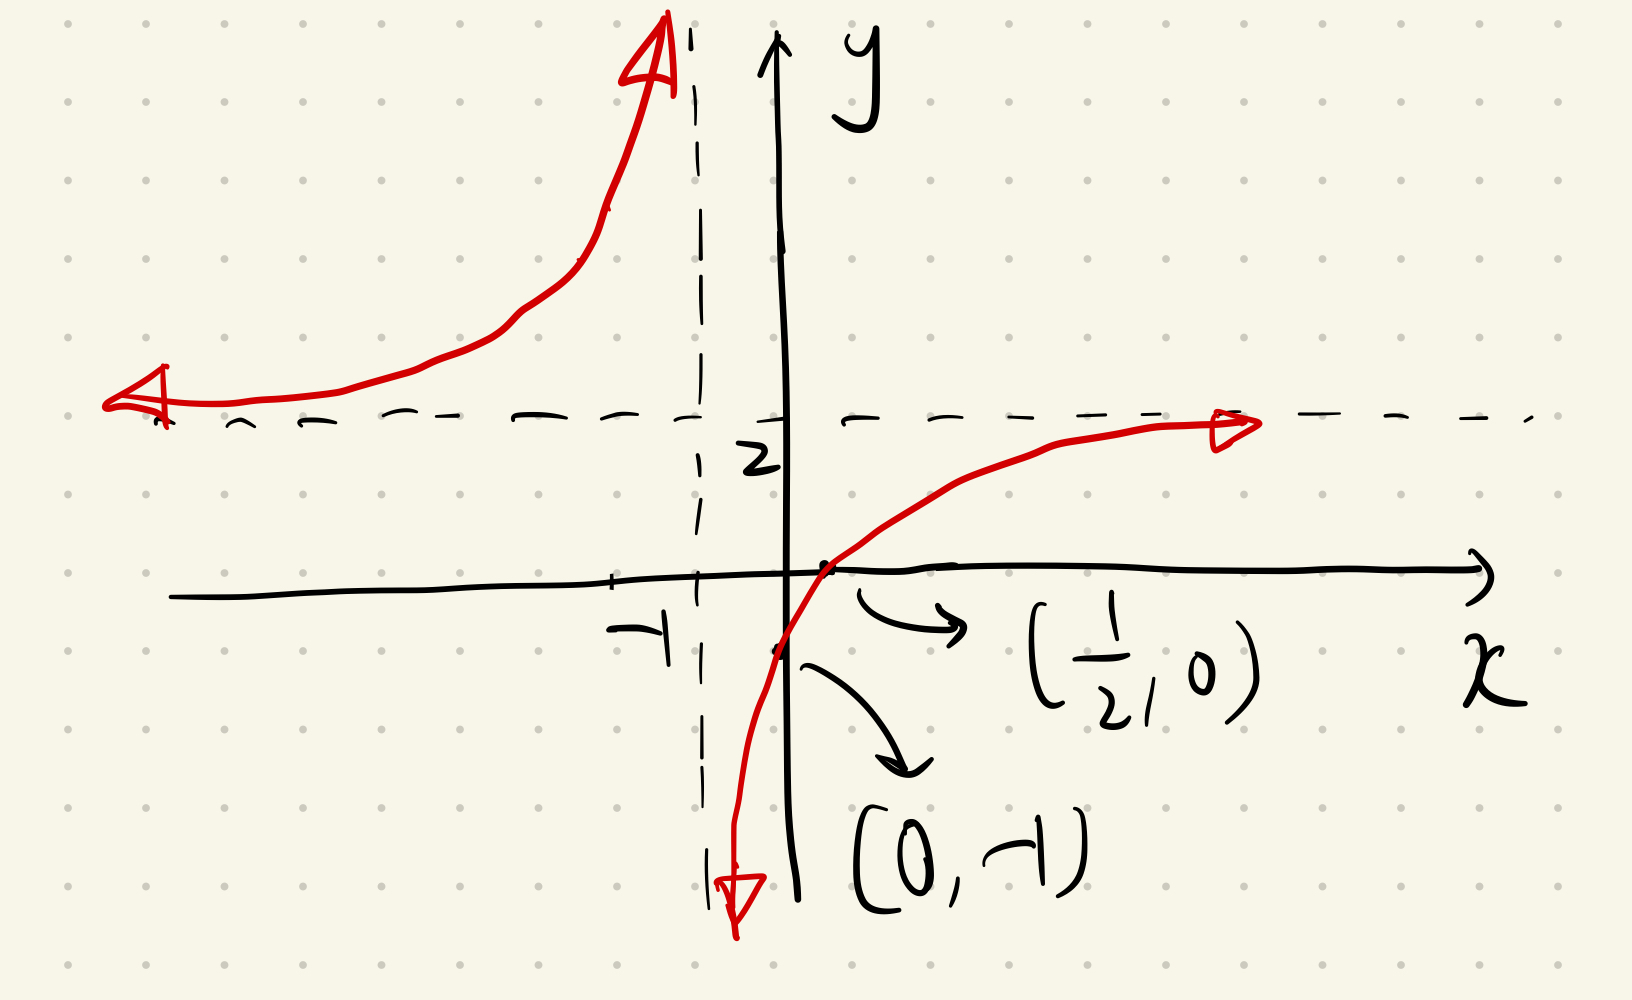
\includegraphics[width = 0.6\textwidth]{figures/chap 05/eg_first_derivative.png}
        \label{fig: eg_first_derivative}
    \end{center}
\end{egsol}

\begin{eg}[]{eg: first_derivative_2}
    Sketch $f(x)=\sqrt{x^3-3x^2+3x}$ using the information of its first derivative.
\end{eg}

\begin{egsol}[]{egsol: first_derivative_2}
    To sketch $f(x)$, we follow the steps of the procedure mentioned above:
    
    \begin{enumerate}
        \item \textit{Domain and behavior at boundaries}: Since there is a square root in the function, $f(x)$ is only defined when the expression in the square root is non-negative. That is,
        \[x^3-3x^2+3x \ge 0\]
        \[x(x^2-3x+3) \ge 0\]
        \[x\Big[\Big(x-\frac{3}{2}\Big)^2+\frac{3}{4}\Big] \ge 0\]
        Since the expression in the middle bracket is always greater than $0$, we conclude that the inequality holds if $x \ge 0$.  That is, the domain of $f(x)$ is $[0, \infty)$.
        
        As of the behavior of $f(x)$ at the boundaries, at the left boundary where $x=0$:
        \[f(0) = 0; \qquad \lim_{x\rightarrow 0^+} f(x) = 0\]
        At the right boundary, i.e. $x \rightarrow \infty$:
        \[\lim_{x\rightarrow \infty} f(x) = \lim_{x\rightarrow \infty} \sqrt{x^3} = \infty\]
        Therefore, $f(x)$ is cut off on the left at $(0,0)$ and goes to $\infty$ on the right as $x \rightarrow \infty$.
        \item \textit{Find discontinuities}: There are no discontinuities in $f(x)$.
        \item \textit{Behavior at discontinuities}: There are no discontinuities in $f(x)$.
        \item \textit{Find and plot critical points}: To find the critical points, we first calculate the derivative:
        \[f'(x) = \frac{(x^3-3x^2+3x)'}{2\sqrt{x^3-3x^2+3x}} = \frac{3x^2-6x+3}{2\sqrt{x^3-3x^2+3x}} = \frac{3}{2\sqrt{x^3-3x^2+3x}}(x-1)^2\]
        Therefore, there is only one critical point, which is $x = 1$ where $f'(1) = 0$.  We can then plot the point $(1,f(1)) = (1,1)$ on the plane.
        \item \textit{Behavior between critical points / discontinuities}: We now determine the sign of $f'(x) = \frac{3}{2\sqrt{x^3-3x^2+3x}}(x-1)^2$ in $[0, 1)$ and $(1, \infty)$, which are all positive.  Therefore, $f(x)$ is strictly increasing in both $[0, 1)$ and $(1, \infty)$.  Note that since $f'(1) = 0$, we must sketch in a way that the tangent line at $x=1$ is horizontal.
        \item \textit{Miscellaneous}: We may try to plot other points, but here we do not see any obvious choices.
    \end{enumerate}
    
    Combining the information above would lead us to the graph below:
    \begin{center}
        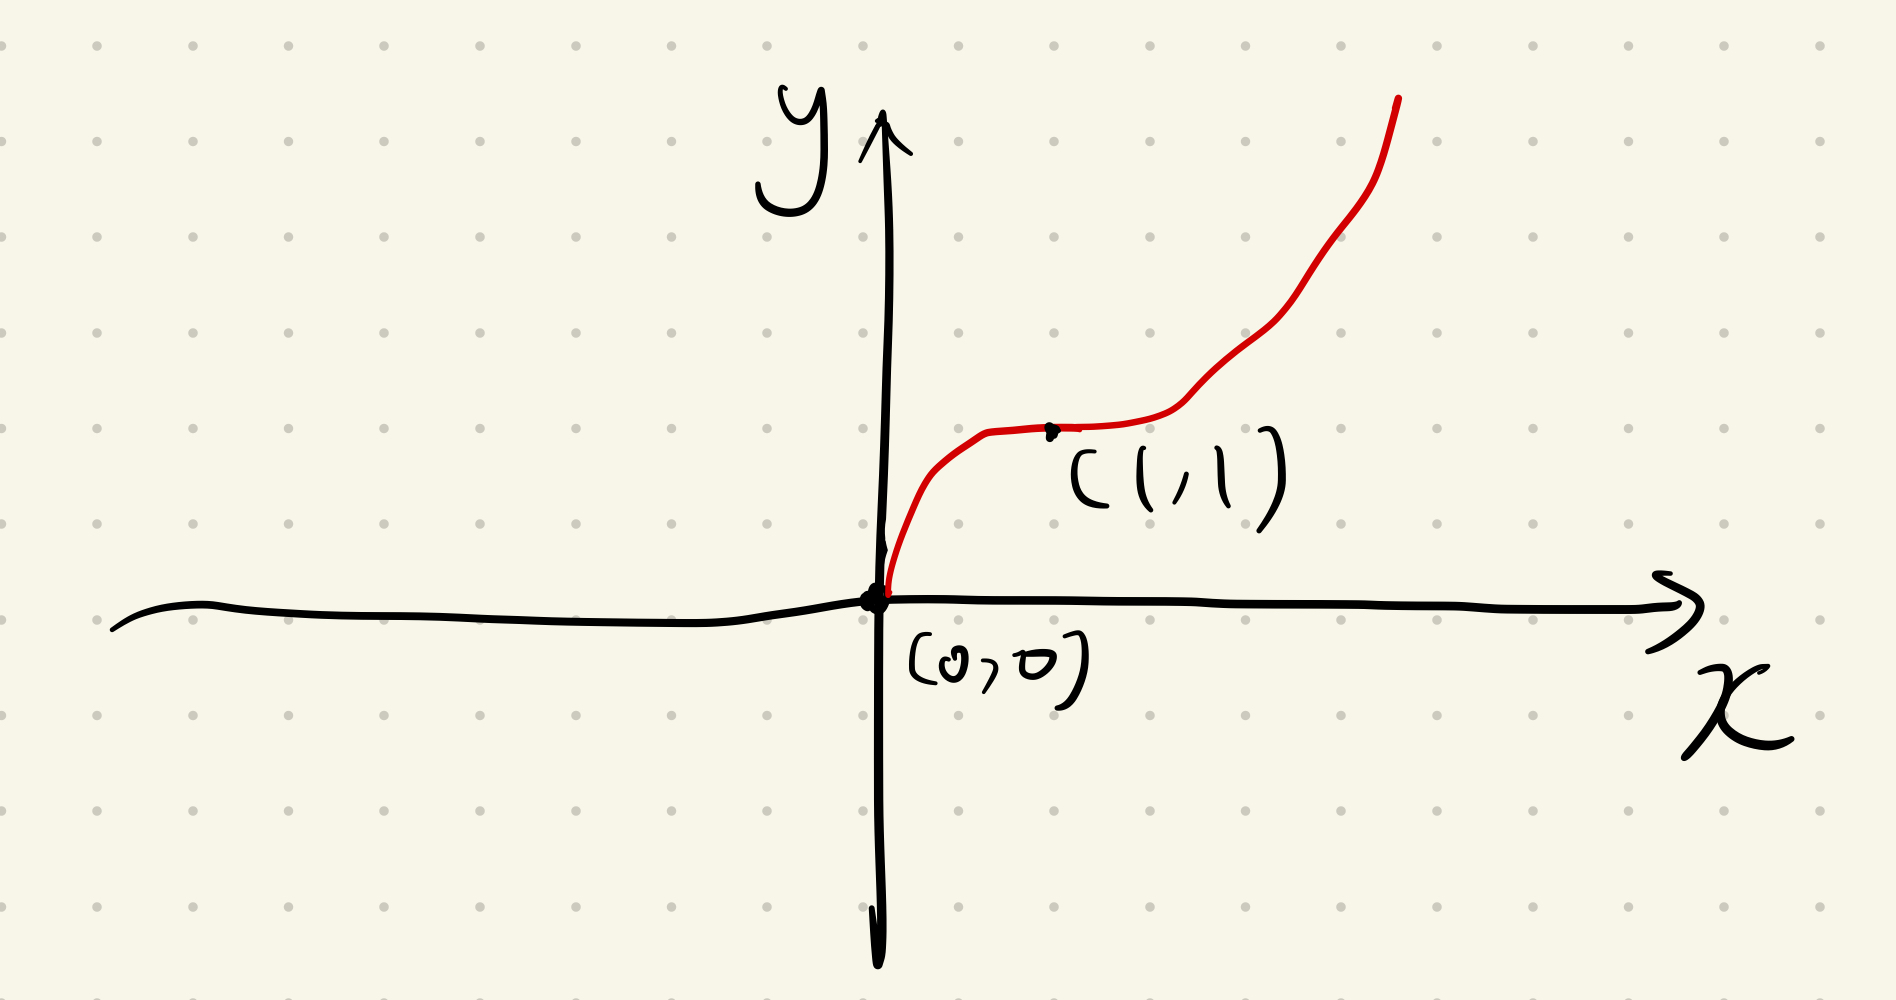
\includegraphics[width = 0.6\textwidth]{figures/chap 05/eg_first_derivative_2.png}
        \label{fig: eg_first_derivative_2}
    \end{center}
\end{egsol}

\begin{ex}[]{ex: first_derivative}
    Sketch $f(x)=\frac{\ln x}{x}$ using the information of its first derivative.
\end{ex}

\begin{exsol}[]{exsol: first_derivative}
    To sketch $f(x)$, we follow the steps of the procedure mentioned above:
    
    \begin{enumerate}
        \item \textit{Domain and behavior at boundaries}: $f(x)$ is only defined if (1) $\ln x$ is defined, i.e. $x > 0$ (2) the denominator $x$ is non-zero, i.e. $x \ne 0$.  Combining these two conditions and we yield the domain of $f(x)$ which is $(0, \infty)$.
        
        As of the behavior of $f(x)$ at the boundaries, at the left boundary where $x=0$, $f(0)$ is undefined, and we have the limit:
        \[\lim_{x\rightarrow 0^+} \frac{\ln x}{x} = \frac{-\infty}{0+} = -\infty\]
        At the right boundary, i.e. $x \rightarrow \infty$, plug-in method yields $\frac{\infty}{\infty}$, so we use the L'Hôpital's rule:
        \[\lim_{x\rightarrow \infty} \frac{\ln x}{x} = \lim_{x\rightarrow \infty} \frac{(\ln x)'}{x'} = \lim_{x\rightarrow \infty} \frac{1/x}{1} = 0\]
        Therefore, $f(x)$ goes to $-\infty$ as $x$ goes to $0$, and as $x \rightarrow \infty$, we have a horizontal asymptote $y = 0$.
        \item \textit{Find discontinuities}: There are no discontinuities in $f(x)$.
        \item \textit{Behavior at discontinuities}: There are no discontinuities in $f(x)$.
        \item \textit{Find and plot critical points}: To find the critical points, we first calculate the derivative:
        \[f'(x) = \frac{(\ln x)'x - (\ln x)x'}{x^2} = \frac{\frac{1}{x}x - \ln x}{x^2} = \frac{1-\ln x}{x^2}\]
        Therefore, there is only one critical point, which is $x = e$ where $f'(e) = 0$.  We can then plot the point $(e,f(e)) = (e,1/e)$ on the plane.
        \item \textit{Behavior between critical points / discontinuities}: We now determine the sign of $f'(x) = \frac{1-\ln x}{x^2}$, which is positive in $(0, e)$ and negative in $(e, \infty)$.  Therefore, $f(x)$ is strictly increasing in $(0, e)$ but strictly decreasing in $(e, \infty)$.
        \item \textit{Miscellaneous}: Since $f(x)$ has an obvious root $x=1$, we can plot $(1,0)$ in the graph.
    \end{enumerate}

    Combining the information above would lead us to the graph below:
    
    \begin{center}
        \includegraphicsex{width = 0.6\textwidth, draft}{width = 0.6\textwidth}{figures/chap 05/ex_first_derivative.png}
        \label{fig: ex_first_derivative}
    \end{center}
\end{exsol}

\subsection{Second Derivative and Concavity}
The second derivative is the derivative of the first derivative, so we can apply Theorem~\ref{thm: derivative_to_monotone} to $f'(x)$ and conclude that $f''(x) > 0$ implies $f'(x)$ is strictly increasing, and $f''(x) < 0$ implies $f'(x)$ is strictly decreasing.  But when $f'(x)$ is strictly increasing / decreasing, what is its implication on the graph of $f(x)$?  To grasp intuition, let's look at the following graph of a function:

\begin{figure}[ht]
    \centering
    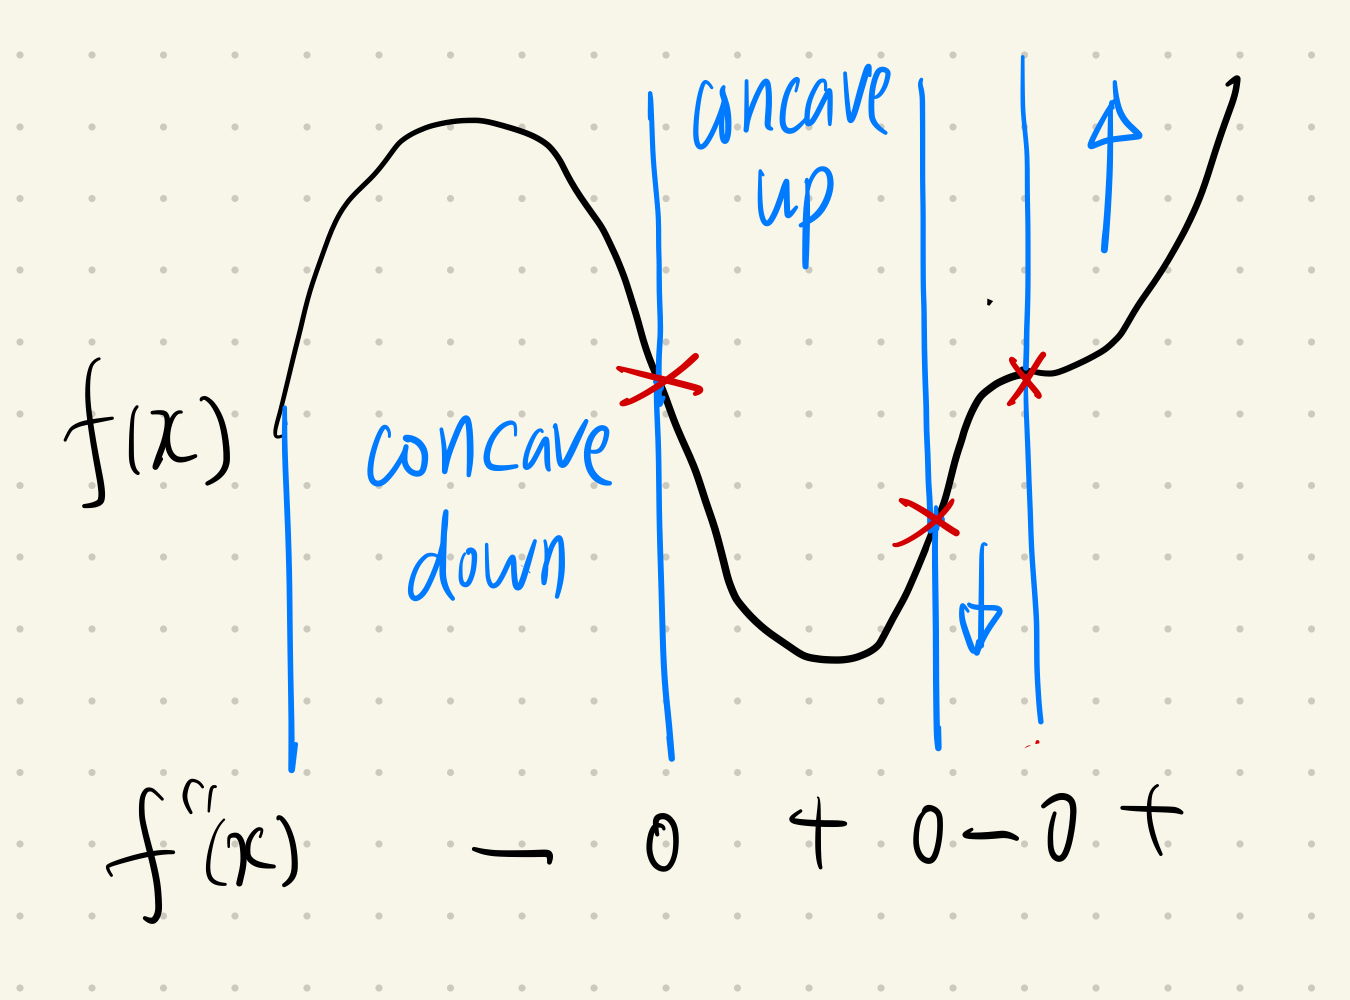
\includegraphics[width = 0.5\textwidth]{figures/chap 05/concavity.png}
    \label{fig: concavity}
\end{figure}

We first investigate the intervals marked as "\textit{concave down}" (or with a downward arrow).  Within these intervals, as $x$ gets larger, the slope of the tangent line decreases, which corresponds to $f'(x)$ \textit{decreasing}.  Note that the graph of $f(x)$ in these intervals resembles a bowl facing down, thus the term "concave down".  

In contrast, within intervals marked as "\textit{concave up}" (or with an upward arrow), the slope of the tangent line increases as $x$ gets larger, which corresponds to $f'(x)$ \textit{increasing}.  The graph of $f(x)$ in these intervals resemble a bowl facing up, thus the term "concave up".

An alternative view of curves concaving up and down is to imagine you are driving a car along the curve to the right.  If the curve is concaving down, then you are turning right along the way.  If the curve is concaving up, then you are turning left along the way.

With the concept of concavity, we can state a theorem very close to Theorem~\ref{thm: derivative_to_monotone}, but for the second derivative:

\begin{theo}[Second derivative and concavity]{thm: second_derivative_to_concavity}
    Suppose a function $f(x)$ is twice differentiable in $(a, b)$, then:
    \[f''(x) > 0, \forall x \in (a, b) \Rightarrow f(x) \text{ is \textit{concave up} in } (a,b)\]
    \[f''(x) < 0, \forall x \in (a, b) \Rightarrow f(x) \text{ is \textit{concave down} in } (a,b)\]
\end{theo}

Note that in the graph, there are points at the border of the concavity intervals (marked with x) where the function transitions from concave down to concave up.  That is, $f''(x)$ has opposite signs at the two sides of the point.  These points are called \textit{inflection points}, which we provide the definition as follows:  

\begin{defi}[]{def: inflection_point}
    A point $x=c$ is the inflection point of $f(x)$ if $f(x)$ is continuous at $x=c$ and the concavity of $f(x)$ changes at the two sides of $x=c$.
\end{defi}

Since $f''(x) > 0$ and $f''(x) < 0$ implies the curve is still concaving up or down around the point, the second derivatives at inflection points should either be $0$ or do not exist.  Therefore, to find inflection points, we can find points where $f''(x) = 0$ or do not exist, then check if $f(x)$ is continuous at these points, and also if $f''(x)$ has different signs at the left and right of these points.  This procedure is analogous to what we're doing in finding critical points.

\begin{remark}
    Concavity has a deep impact on the complexity of finding the maximum and minimum of a function using algorithms (eg. Newton's method).  If the whole function is concave up (down), then finding the minimum (maximum) of the function will be relatively easy, since the function is shaped like a big valley (peak) with one minimum (maximum), and you can find the solution easily with the help of derivatives.  However, if the function is somewhere concave up and somewhere concave down, then the curve of the function can be rugged, and you may have a hard time finding the minimum or maximum if your choice of initial value is sub-optimal.
\end{remark}

\begin{figure}[ht]
    \centering
    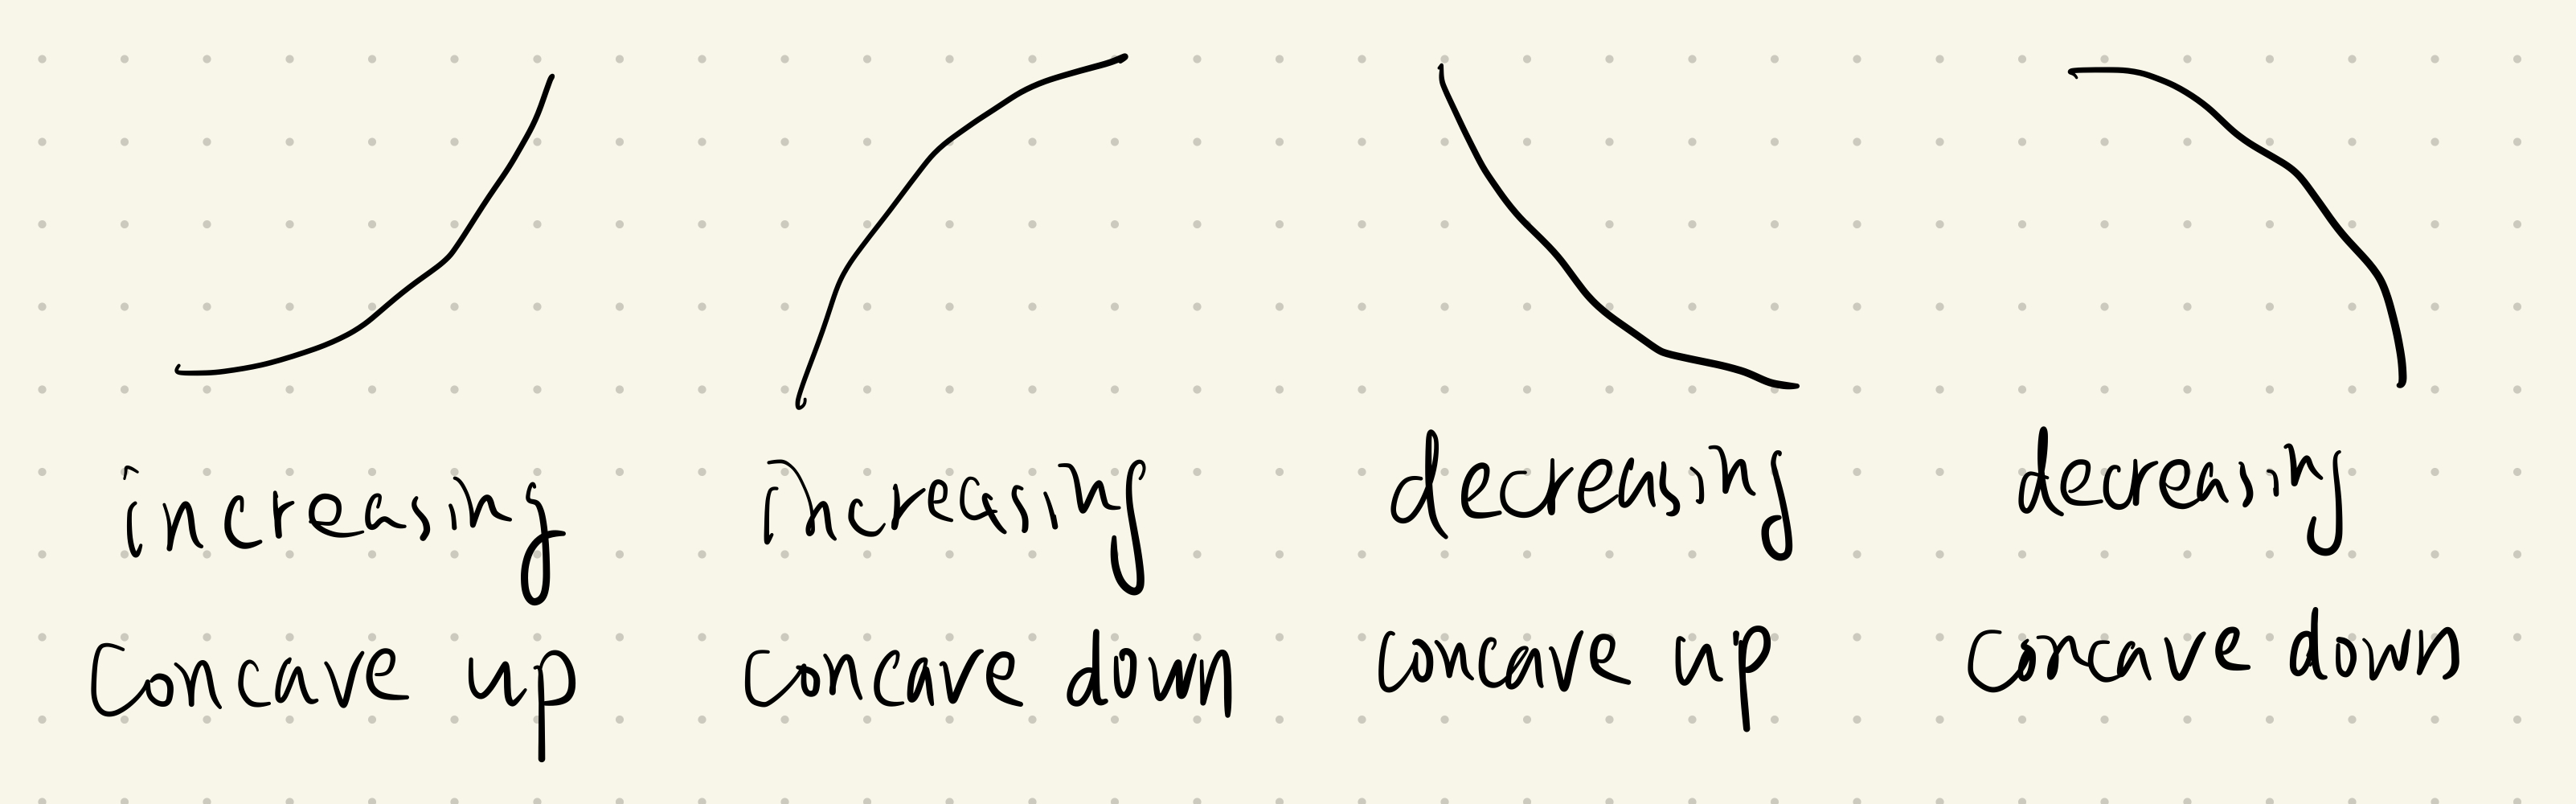
\includegraphics[width = 0.75\textwidth]{figures/chap 05/concavity_monotone.png}
    \label{fig: concavity_monotone}
\end{figure}

A word of caution is that the increasing / decreasing of a function is related to its \textit{first} derivative, and the concavity of a function is related to its \textit{second} derivative, so be careful not to mix up these two qualities of a function.  In fact, as the graph above shows, every combination between increasing / decreasing and concaving up / down is possible.

To incorporate the information of second derivatives into curve sketching, we can try finding all inflection points and incorporate the concavity of the function into our sketch after we're done with first derivatives.  We will demonstrate this with one example before ending this section. 

\begin{eg}[]{eg: second_derivative}
    Sketch $f(x) = xe^{4x}$ using the information of its first and second derivatives.
\end{eg}

\begin{egsol}[]{egsol: second}
    To sketch $f(x)$, we follow the steps of the procedure mentioned in the last subsection, but adding the inference from second derivatives:
    
    \begin{enumerate}
        \item \textit{Domain and behavior at boundaries}: The domain of $f(x)$ is $\mathbb{R}$, so we need to assess its behavior as $x \rightarrow -\infty$ and $x \rightarrow \infty$ (L'Hôpital's rule is used for $x \rightarrow -\infty$ since plug-in method leads to $-\infty \cdot 0$). 
        \[\lim_{x \rightarrow -\infty} xe^{4x} = \lim_{x \rightarrow -\infty} \frac{x}{e^{-4x}} = \lim_{x \rightarrow -\infty} \frac{x'}{(e^{-4x})'} = \lim_{x \rightarrow -\infty} \frac{1}{-4e^{-4x}} = 0\]
        \[\lim_{x \rightarrow \infty} xe^{4x} = \infty\]
        Therefore, on the left, $f(x)$ has a horizontal asymptote $y=0$; on the right, $f(x)$ goes to $\infty$ as $x$ goes to $\infty$.
        \item \textit{Find discontinuities}: There are no discontinuities in $f(x)$.
        \item \textit{Behavior at discontinuities}: There are no discontinuities in $f(x)$.
        \item \textit{Find and plot critical points}: To find the critical points, we first calculate the derivative:
        \[f'(x) = (x)'e^{4x} + x(e^{4x})' = e^{4x} + 4xe^{4x} = (4x+1)e^{4x}\]
        Therefore, there is only one critical point, which is $x = -\frac{1}{4}$ where $f'\big(-\frac{1}{4}\big) = 0$.  We can then plot the point $\big(-\frac{1}{4},f\big(-\frac{1}{4}\big)\big) = \big(-\frac{1}{4},-\frac{1}{4e})$ on the plane.
        \item \textit{Behavior between critical points / discontinuities}: We now determine the sign of $f'(x) = (4x+1)e^{4x}$ in $\big(-\infty, -\frac{1}{4}\big)$ and $\big(-\frac{1}{4}, \infty\big)$.  Since $e^{4x}$ is always non-negative, the sign of $f'(x)$ depends on the sign of $(4x+1)$.  Therefore, $f(x)$ is strictly decreasing in $\big(-\infty, -\frac{1}{4}\big)$ and strictly increasing in $\big(-\frac{1}{4}, \infty\big)$.
        \item \textit{Plot inflection points and assess concavity}: To find the inflection points, we calculate the second derivative:
        \[f''(x) = (4x+1)'e^{4x} + (4x+1)(e^{4x})' = 4e^{4x} + 4(4x+1)e^{4x} = (16x+8)e^{4x}\]
        Therefore, the only candidate for the inflection point is $x = -\frac{1}{2}$ where $f''\big(-\frac{1}{2}\big) = 0$.  
        
        To verify $x = -\frac{1}{2}$ is indeed an inflection point, we have to show that $f''(x)$ has opposite signs at different sides of $x = -\frac{1}{2}$:
        \[x < -\frac{1}{2} \Rightarrow 16x+8 < 0 \Rightarrow f''(x) = (16x+8)e^{4x} < 0\]
        \[x > -\frac{1}{2} \Rightarrow 16x+8 > 0 \Rightarrow f''(x) = (16x+8)e^{4x} > 0\]
        Therefore, $x = -\frac{1}{2}$ is an inflection point and we plot $\big(-\frac{1}{2},f\big(-\frac{1}{2}\big)\big) = \big(-\frac{1}{2},-\frac{1}{2e^2})$ on the graph, and keep in mind that $f(x)$ is concave down when $x < -\frac{1}{2}$ and concave up when $x > -\frac{1}{2}$.
        \item \textit{Miscellaneous}: An easy point to plot is $(0, f(0)) = (0, 0)$, so we add it to the graph
    \end{enumerate}
    
    Combining the information above would lead us to the graph below:
    \begin{center}
        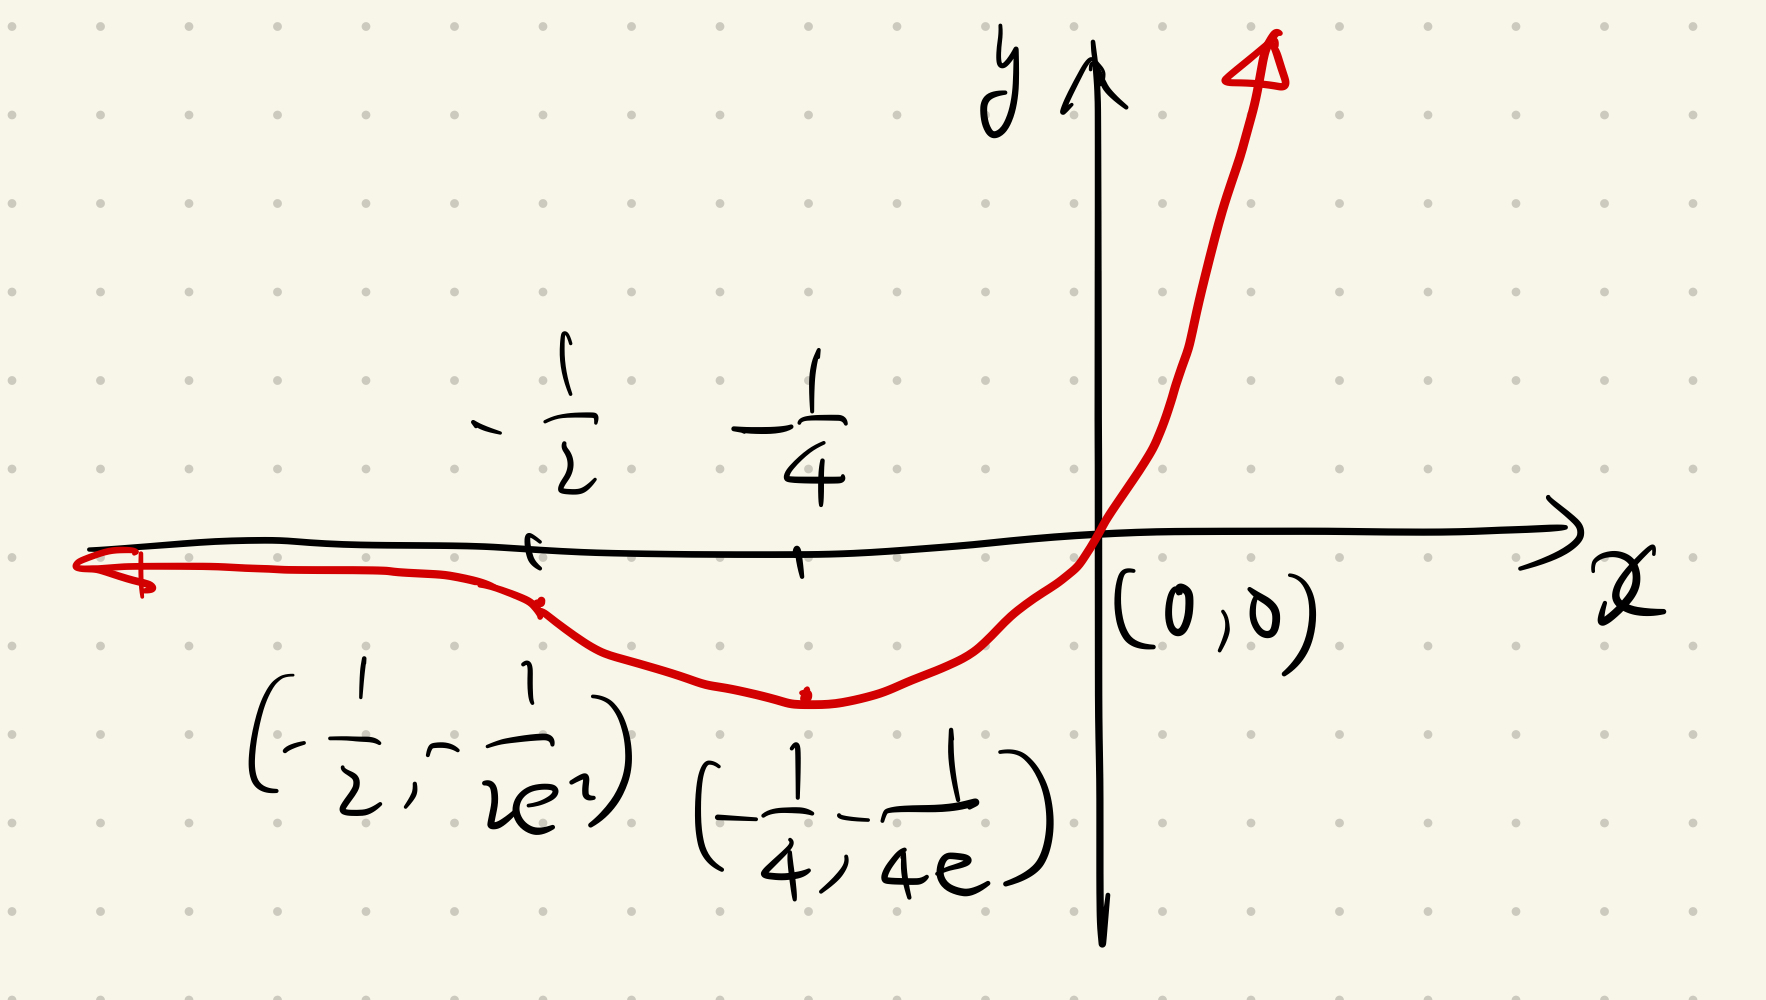
\includegraphics[width = 0.6\textwidth]{figures/chap 05/eg_second_derivative.png}
        \label{fig: eg_second_derivative}
    \end{center}
\end{egsol}

\pagebreak
\section{Finding the Extrema of a Function}

Another important use of derivatives is to determine the maximum or minimum of a function within an interval of input.  Since maxima and minima are where the function values are at their extremes, we also term them as \textit{extrema}.  Before we look into how to find the extrema of a function, we first look at the two types of extrema, \textbf{global (absolute) extrema} and \textbf{local (relative) extrema}.  

\subsection{Definition of Extrema}

Global extrema are easy to understand: it is the maximal (minimal) value the function can output.  In mathematical terms, if a function $f$ is attaining value $f(c)$ at $x=c$, and any other possible function values are less than or equal to $f(c)$, then we say $f(x)$ has a global maximum at $x=c$.  Similar arguments can be made for global minimum.  

Local extrema are a little bit more involved: If a function $f$ is attaining value $f(c)$ at $x=c$ so that all inputs \textit{around} $x=c$ are giving values less than or equal to $f(c)$, then we say $f(x)$ has a local maximum at $x=c$.  Similar arguments can be made for global maximum.  Note that here we are using the term \textit{around} in a sense that we must be able to compare $f(c)$ with function values with input less than $c$ and greater than $c$.  Therefore, the local extrema can never attained at $x=c$ if $x=c$ is at the boundary of the interval of input, since we cannot compare $f(c)$ with function values evaluated at both sides of $c$.

\begin{figure}[ht]
    \centering
    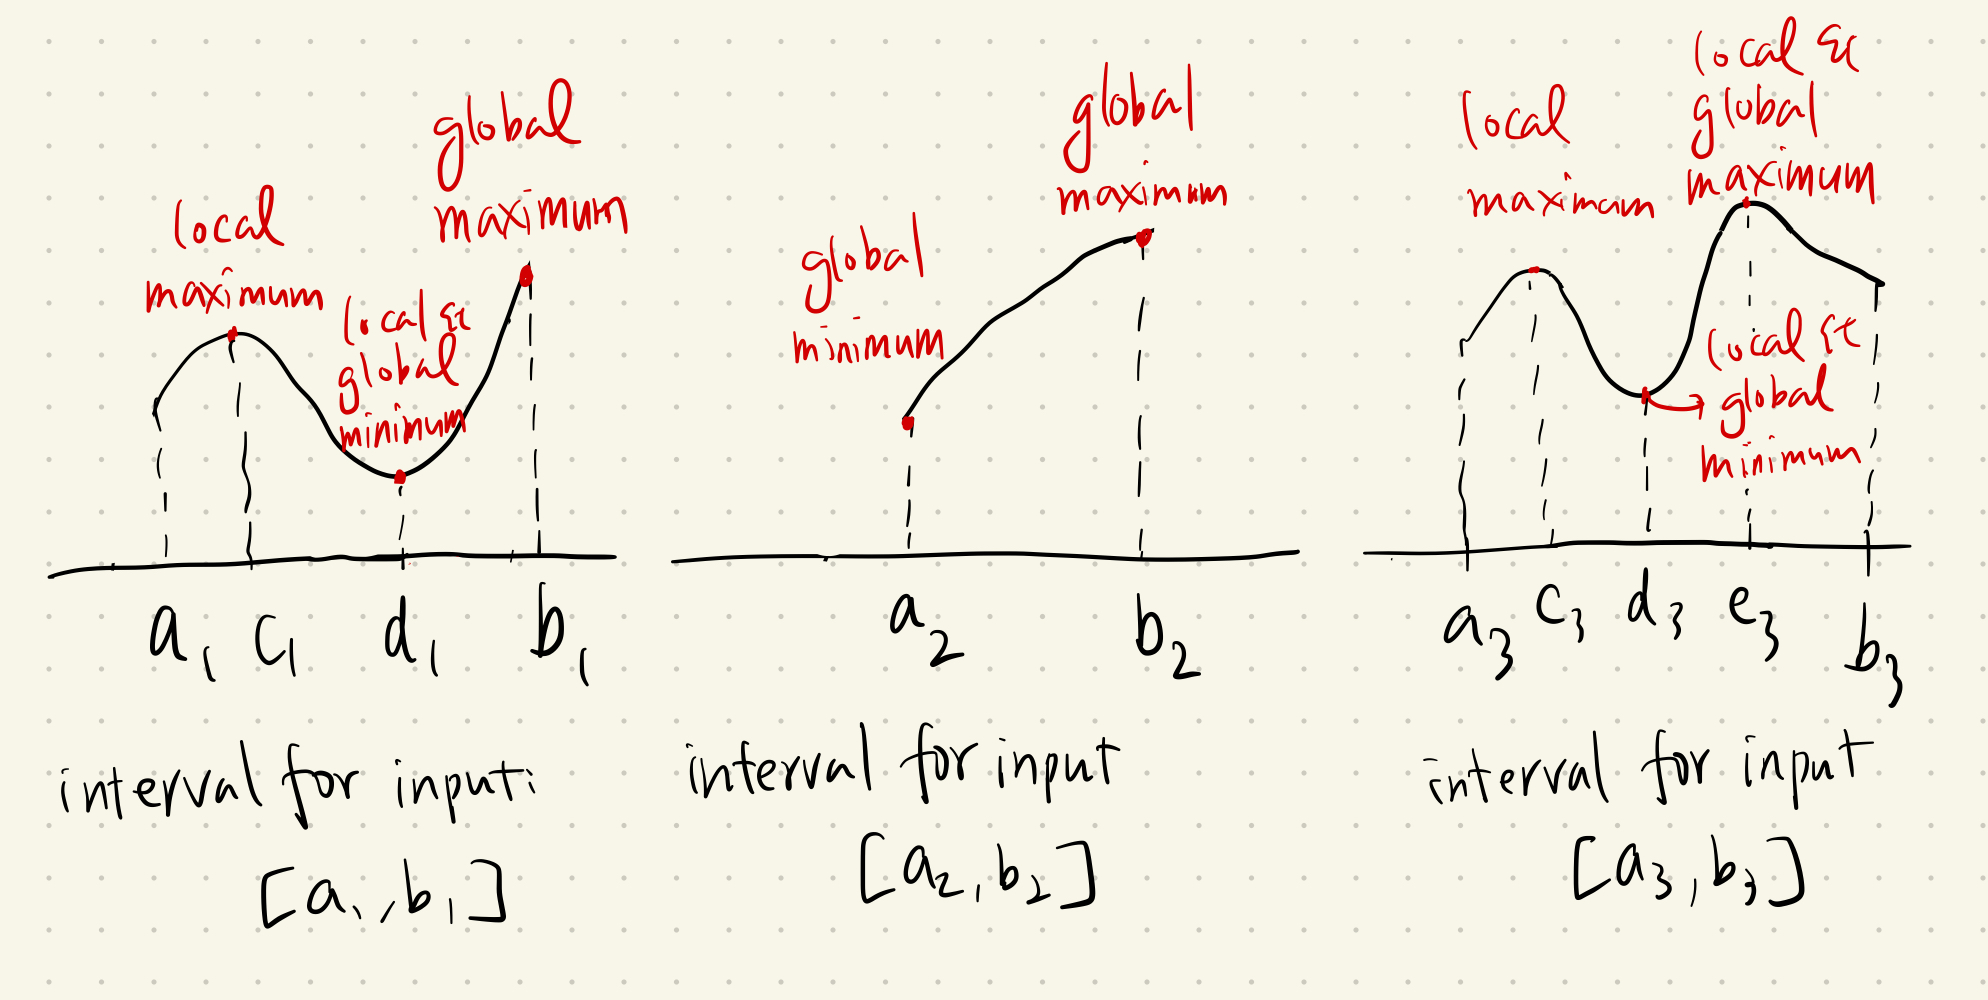
\includegraphics[width = \textwidth]{figures/chap 05/extrema.png}
    \label{fig: extrema}
\end{figure}

We can put these intuition to the test with the graph above:
\begin{itemize}
    \item Left panel: The global maximum is attained at $x=b_1$ since it produces the largest output among inputs within $[a_1, b_1]$.  However, $f(b_1)$ is \textit{not} a local maximum since $b_1$ is at the boundary of $[a_1, b_1]$, so we can't compare $f(b_1)$ with function values evaluated at $x > b_1$.  On the other hand, we have a local maximum attained at $x = c_1$, but it is not a global maximum since $f(c_1) < f(b_1)$.  Local and global extrema can also be attained at the same input, such as $x=d_1$ here where local and global minimum are both attained.
    \item Middle panel: Local extrema do not necessarily exist.  In this example, there are no local extrema for $f(x)$ within $[a_2, b_2]$, but the global extrema still exist.
    \item Right panel: Although there can be at most one global maximum and one global minimum, it is possible to have multiple local maxima or multiple local minima.  In this example, there are two local maxima for $f(x)$ in $[a_3, b_3]$, one attained at $x=c_3$ and the other attained at $x = e_3$.
\end{itemize}

We end this subsection by providing a formal definition of extrema.

\begin{defi}[Extrema]{def: extrema}
    Suppose $x=c$ is in the domain of $f(x)$, let $I_0$ be an interval for input where $c \in I_0$
    \begin{itemize}
        \item $f(x)$ has a \textbf{global (absolute) maximum} at $x=c$ within $I_0$ if $f(x) \le f(c), \forall x \in I_0$ 
        \item $f(x)$ has a \textbf{global (absolute) minimum} at $x=c$ within $I_0$ if $f(x) \ge f(c), \forall x \in I_0$ 
        \\
        \item $f(x)$ has a \textbf{local (relative) maximum} at $x=c$ within $I_0$ if there exists an open interval $I \subset I_0$ where $c \in I$ and $f(x) \le f(c), \forall x \in I$ 
        \item $f(x)$ has a \textbf{local (relative) minimum} at $x=c$ within $I_0$ if there exists an open interval $I \subset I_0$ where $c \in I$ and $f(x) \ge f(c), \forall x \in I$ 
    \end{itemize}
\end{defi}

\subsection{Existence and Identification of Global Extrema}

When we are trying to maximize or minimize a function, what we care about is the \textit{global} extrema.  Therefore, for the maximization or minimization to make sense, we must make sure that the global extrema exist.  However, global extrema do not always exist.  For example, in the following graph, both the global maximum and minimum do not exist.

\begin{figure}[ht]
    \centering
    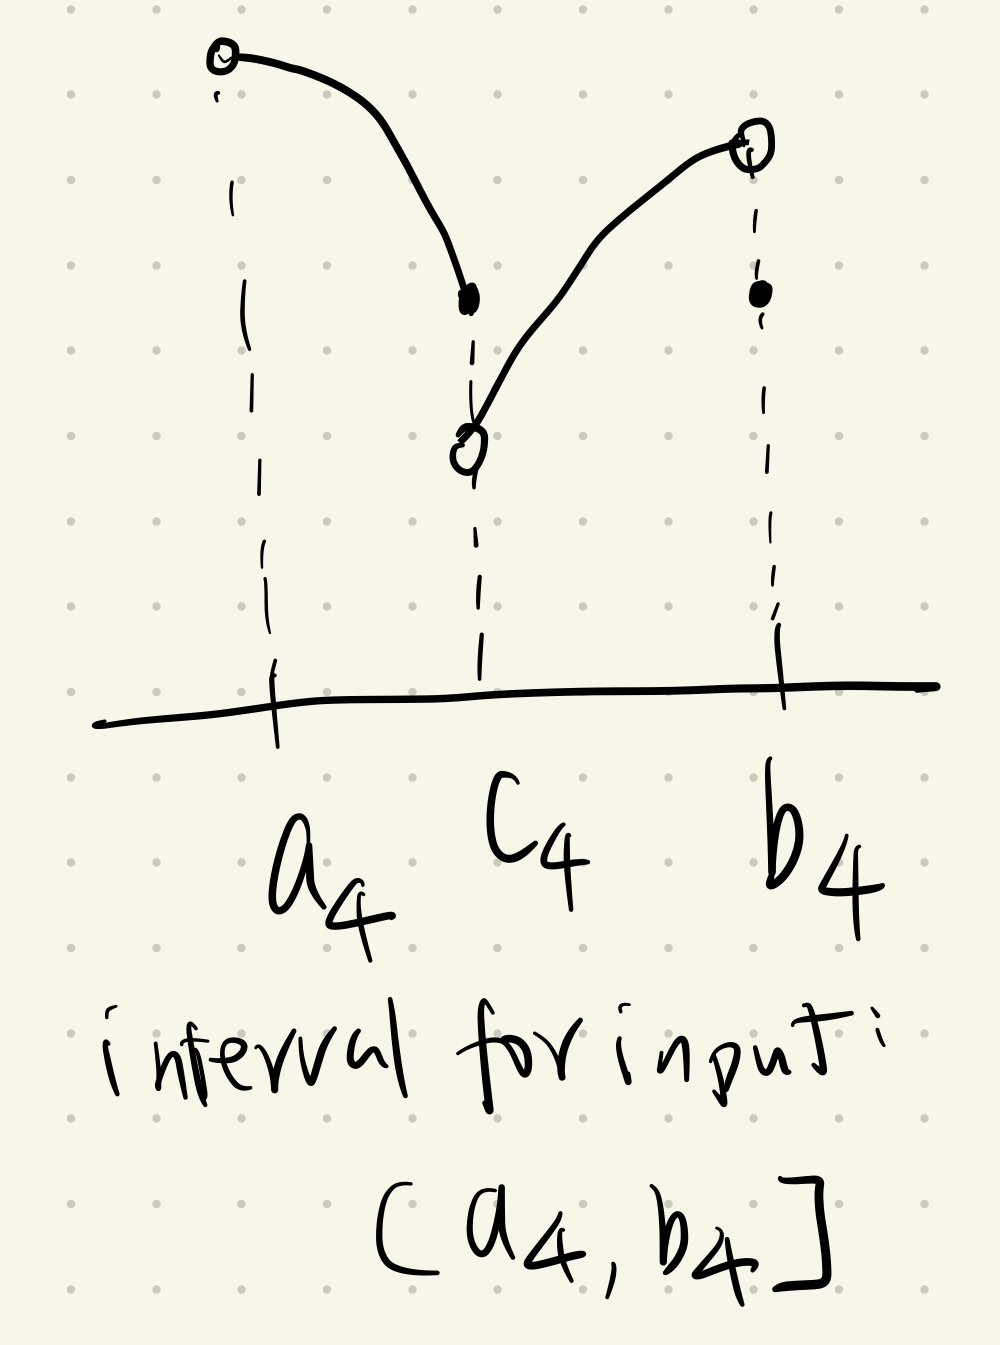
\includegraphics[width = 0.25\textwidth]{figures/chap 05/global_extrema_dne.png}
    \label{fig: global_extrema_dne}
\end{figure}

Fortunately, if we focus on only \textit{continuous} functions with a \textit{closed interval} for input, the global extrema always exists and we can safely do maximization or minimization.  This fact can be summarized in the \textbf{Extreme Value Theorem} below.

\begin{theo}[Extreme Value Theorem]{thm: evt}
    Suppose $f(x)$ is continuous in $[a, b]$, then there exists $x_M, x_m \in [a, b]$ so that $f(x_M)$ is the global maximum of $f(x)$ in $[a, b]$, and $f(x_m)$ is the global minimum of $f(x)$ in $[a, b]$. 
\end{theo}

Now we know the global extrema exist as long as we are dealing with a continuous function within a closed interval for input.  However, knowing their existence is not enough: we want to know where the global extrema is obtained.  To search for global extrema, we first make an important observation: if the global maximum (minimum) is not obtained at the boundaries of the closed interval, then it should also be a local maximum (minimum), since it is larger (smaller) than the function values \textit{around} it.  Therefore, the global extrema can only be attained at the boundaries or at where the local extrema are attained.  This fact is useful since we can locate the local extrema using the following theorem by \textit{Pierre de Fermat}:

\begin{theo}[Fermat's Interior Extremum Theorem]{thm: fermat}
    Suppose $f(x)$ attains local extremum at $x=x_0 \in (a, b)$.  If $f(x)$ is differentiable at $x = x_0$, then $f'(x_0) = 0$.
\end{theo}

An implication of this theorem is that if $f(x)$ has local extremum at $x = x_0$, then either $f'(x_0)=0$ or $f'(x_0)$ does not exist.  Therefore, we can find all candidates of local extremum by identifying all points where the first derivative equals to zero or does not exist, which are the \textit{critical points} of $f(x)$ as we have defined earlier.  An important logic here is that all local extrema occur at critical points, but not all critical points has a local extremum attached to them.  An evident example is $x=x_3$ in Figure~\ref{fig: critical_points}.

Summarizing up, we can find the global extrema of a continuous function $f(x)$ within a close interval $[a, b]$ using the following steps:

\begin{enumerate}
    \setcounter{enumi}{-1}
    \item Verify that $f(x)$ is indeed continuous in $[a, b]$.
    \item Find all the critical points of $f(x)$ in $(a, b)$.
    \item Evaluate $f(x)$ at $a$, $b$, and all the critical points.
    \item Compare the function values: the largest one is the global maximum, and the smallest one is the global minimum.
\end{enumerate}

This procedure is pretty straightforward, which we will demonstrate with a couple of examples. 

\begin{eg}[]{eg: extrema_1}
    Find the global extrema for $f(x) = 2x^3 - 3x^2 - 12x + 5$ in $x \in [-3, 3]$.
\end{eg}

\begin{egsol}[]{egsol: extrema_1}
    We follow the procedure mentioned above:
    \begin{enumerate}
        \setcounter{enumi}{-1}
        \item Since $f(x)$ is a polynomial, it is continuous in $\mathbb{R}$ and thus in $[3, 3]$.
        \item To find the critical points for $f(x)$ in $[-3, 3]$, we first obtain its derivative:
        \[f'(x) = 6x^2-6x-12 = 6(x^2-x-2) = 6(x+1)(x-2)\]
        Therefore, the points where $f'(x) = 0$ are $x = -1$ and $x = 2$, which are both in $[-3, 3]$ and thus our desired critical points.
        \item We evaluate $f(x)$ at $-3, 3, -1, 2$ and yield
        \[f(-3) = -40 \qquad f(3) = -4 \qquad f(-1) = 12 \qquad f(2) = -15\]
        \item Since $-40 = f(-3) < f(2) < f(3) < f(-1) = 12$, the global minimum is $-40$ attained at $x=-3$, and the global maximum is $12$ attained as $x = -1$.
    \end{enumerate}
\end{egsol}

\begin{eg}[]{eg: extrema_2}
    Find the global extrema for $f(x) = 2x + \cos(4x)$ in $x \in \big[-\frac{\pi}{2}, \frac{\pi}{2}\big]$.
\end{eg}

\begin{egsol}[]{egsol: extrema_2}
    We follow the procedure mentioned above:
    \begin{enumerate}
        \setcounter{enumi}{-1}
        \item Since $x$ and $\cos x$ are all continuous in $\mathbb{R}$, $f(x)$ is continuous in $\big[-\frac{\pi}{2}, \frac{\pi}{2}\big]$.
        \item To find the critical points for $f(x)$ in $\big[-\frac{\pi}{2}, \frac{\pi}{2}\big]$, we first obtain its derivative:
        \[f'(x) = 2-4 \sin 4x = 2(1 - 2 \sin 4x)\]
        Therefore, the points where $f'(x) = 0$ are where $\sin 4x = \frac{1}{2}$.  Since $x \in \big[-\frac{\pi}{2}, \frac{\pi}{2}\big]$, we have $4x \in [-2\pi, 2\pi]$, so there are four solutions for $\sin 4x = \frac{1}{2}$: $4x = \frac{\pi}{6}$ or $\frac{5\pi}{6}$ or $\frac{\pi}{6}-2\pi$ or $4x = \frac{5\pi}{6} - 2\pi$.  That is, $x = \frac{\pi}{24}$ or $\frac{5\pi}{24}$ or $-\frac{11\pi}{24}$ or $-\frac{7\pi}{24}$
        \item We evaluate $f(x)$ at $-\frac{\pi}{2}, \frac{\pi}{2}, \frac{\pi}{24}, \frac{5\pi}{24}, -\frac{11\pi}{24}, -\frac{7\pi}{24}$ and yield
        
        \begin{center}
            \begin{tabular}{ll}
                $f\big(-\frac{\pi}{2}\big) = -\pi+1 \approx -2.142$ &  $f\big(\frac{\pi}{2}\big) = \pi+1 \approx 4.142$\\
                $f\big(\frac{\pi}{24}\big) = \frac{\pi}{12} + \frac{\sqrt{3}}{2} \approx 1.128$ & $f\big(\frac{5\pi}{24}\big) = \frac{5\pi}{12} - \frac{\sqrt{3}}{2} \approx 0.443$\\
                $f\big(-\frac{11\pi}{24}\big) = -\frac{11\pi}{12} + \frac{\sqrt{3}}{2} \approx -2.014$ & $ f\big(-\frac{7\pi}{24}\big) = -\frac{7\pi}{12} - \frac{\sqrt{3}}{2} \approx -2.699$
            \end{tabular}
        \end{center}
        \item Since $f\big(-\frac{7\pi}{24}\big) < f\big(-\frac{\pi}{2}\big) < f\big(-\frac{11\pi}{24}\big) < f\big(\frac{5\pi}{24}\big) < f\big(\frac{\pi}{24}\big) < f\big(\frac{\pi}{2}\big)$, the global minimum is $-\frac{7\pi}{12} - \frac{\sqrt{3}}{2}$ attained at $x=-\frac{7\pi}{24}$, and the global maximum is $\pi+1 $ attained as $x = \frac{\pi}{2}$.
    \end{enumerate}
\end{egsol}

\subsection{Identification of Local Extrema}

In the previous subsection, we used Fermat's Interior Extremum Theorem to identify potential points where local extrema may be attained for a function, and concluded that we only needed to look at the critical points of the function.  However, we did not look into the behavior of the function around these critical points.  That is, we do not know if these critical points represent local maximum, local minimum, or neither of them.  As we will show in the next two theorems, we can parse out these scenarios using the function's first and second derivatives, with the intuition brought from what we have learned in curve sketching.

\begin{theo}[First Derivative Test]{thm: first_deriv_test}
    Suppose $x = c$ is a critical point of $f(x)$ where $f'(c) = 0$, then
    \begin{enumerate}
        \item If $f'(x) > 0$ at the left of $x = c$ and $f'(x) < 0$ at the right of $x = c$, then local maximum is attained at $x=c$.
        \item If $f'(x) < 0$ at the left of $x = c$ and $f'(x) > 0$ at the right of $x = c$, then local minimum is attained at $x=c$.
        \item If $f'(x)$ have the same sign on both sides of $x = c$, then $x = c$ does not represent any local extrema.
    \end{enumerate}
\end{theo}

\begin{theo}[Second Derivative Test]{thm: second_deriv_test}
    Suppose $x = c$ is a critical point of $f(x)$ where $f'(c) = 0$ and $f''(x)$ is continuous around $x = c$, then
    \begin{enumerate}
        \item If $f''(c) < 0$, then local maximum is attained at $x=c$.
        \item If $f''(c) > 0$, then local minimum is attained at $x=c$.
        \item If $f''(c) = 0$, then $x = c$ can represent local maximum, local minimum or neither.
    \end{enumerate}
\end{theo}

We look at some examples in the following graph, where $x=0$ is a critical point for all of the functions.  With $y=x^2$ and $y=x^4$, the first derivative is negative when $x<0$ and positive when $x>0$, therefore the function is decreasing when $x < 0$ and increasing when $x > 0$, so $x=0$ represents the position of a local minimum.  Similiar arguments can be  made for $y=-x^2$ and $y=-x^4$, only now $x=0$ represents the position of a local maximum.  For $y = x^3$, the first derivative is positive at both sides of $x=0$, so $x=0$ does not represent local extremum.  

For second derivatives, we see that $y=x^2$ has a positive second derivative at $x=0$, meaning that the function is concave up at $x=0$, so $x=0$ represents a local minimum.  The same can be said for $y=-x^2$.  However, from $y=x^3$, $y=x^4$ and $y=-x^4$ we can see that a second derivative of zero does not give us information on whether $x=0$ represents local maximum, local minimum or neither.  We will have to rely on the first derivative to know for sure.


\begin{figure}[ht]
    \centering
    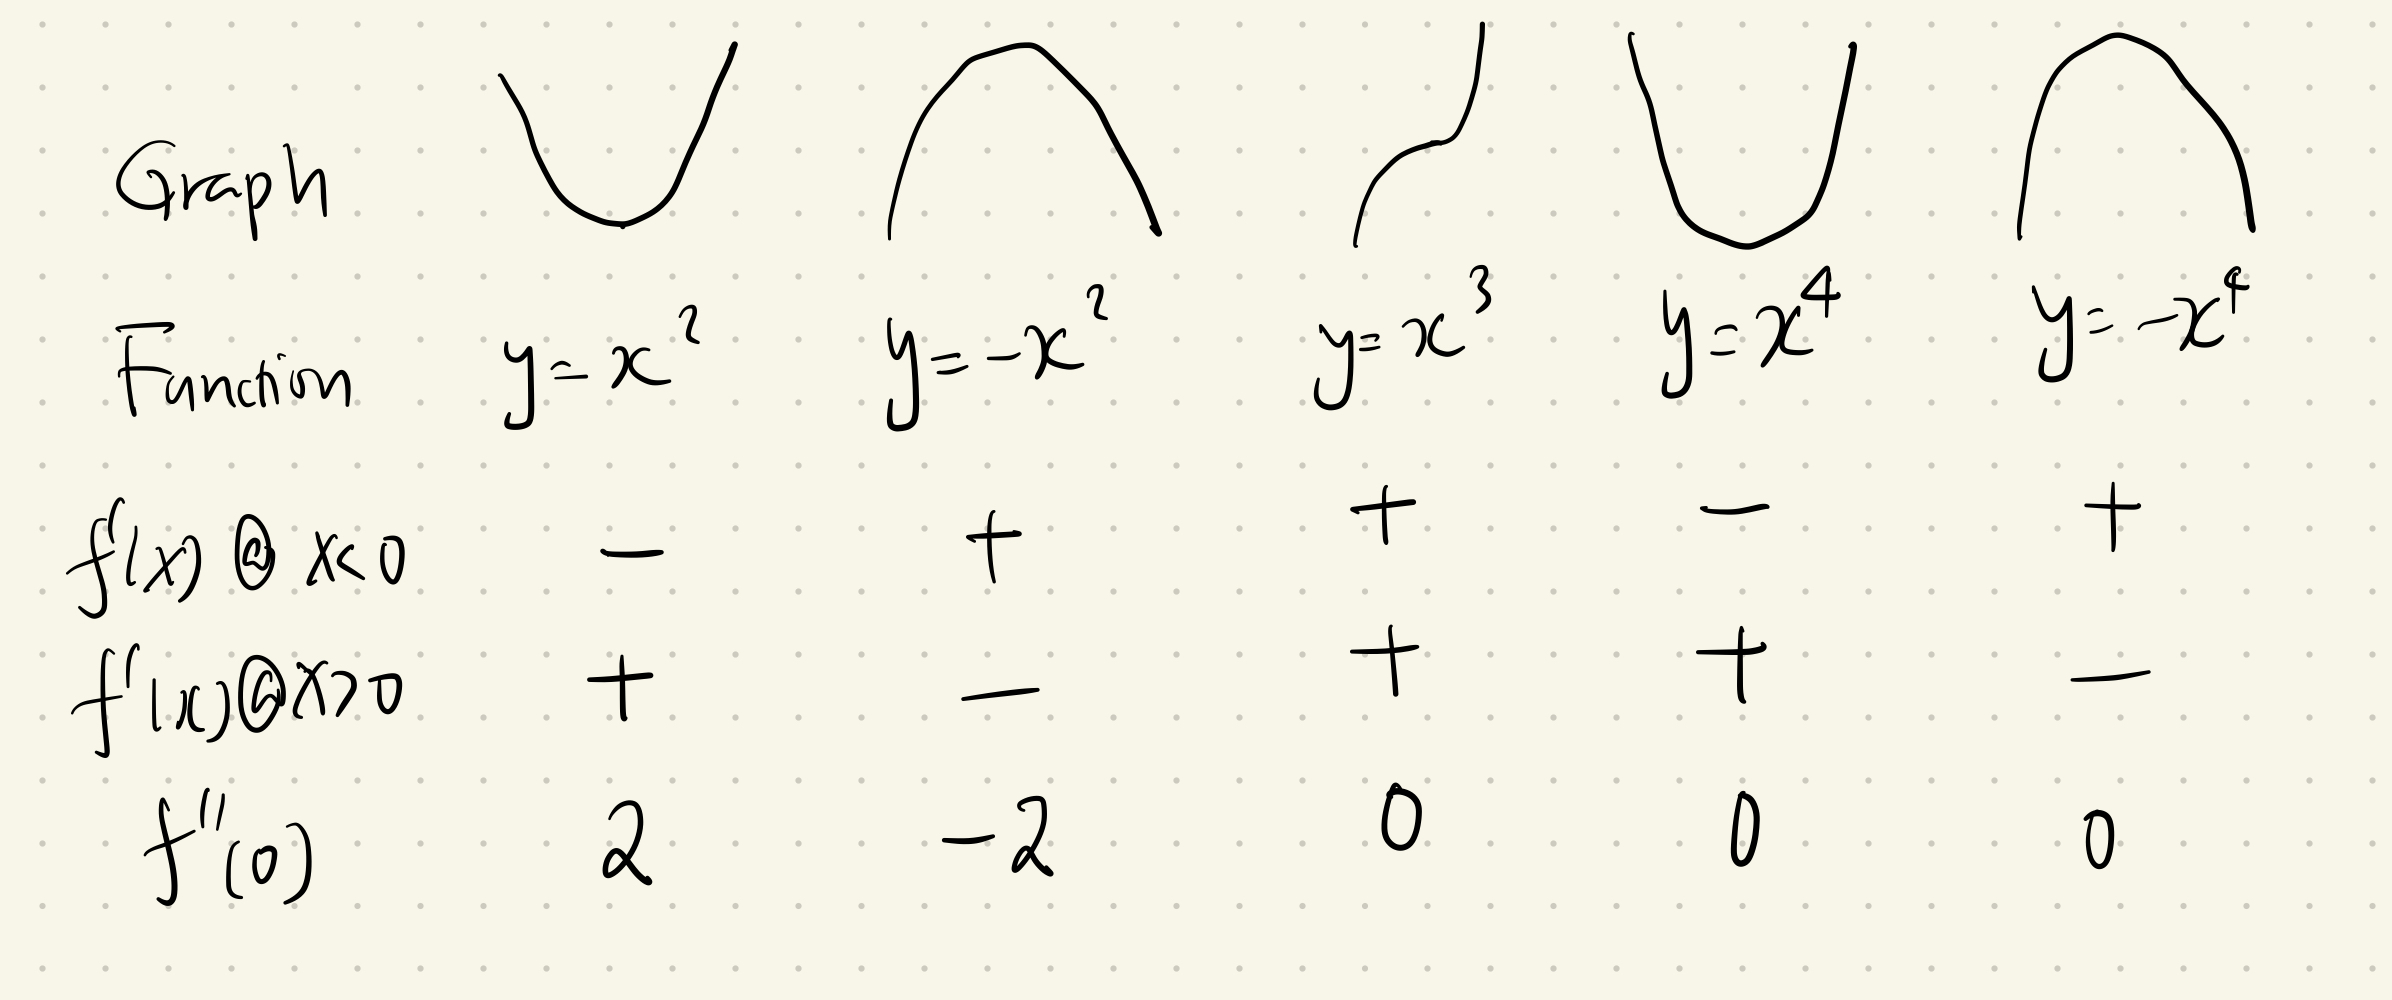
\includegraphics[width = \textwidth]{figures/chap 05/first_second_deriv_test.png}
    \label{fig: first_second_deriv_test}
\end{figure}

We end this section with an example:

\begin{eg}[]{eg: first_second_deriv_test}
    Find all local extrema for $f(x) = 3x^5 - 5x^3 + 30$, and argue if they are local minima or local maxima.
\end{eg}

\begin{egsol}[]{egsol: first_second_deriv_test}
    To locate the local extrema of $f(x)$, we first find the critical points for $f(x)$, which are where $f'(x)$ is undefined or zero.  We first obtain the first derivative:
    \[f'(x) = 15x^4-15x^2 = 15x^2(x^2-1) = 15(x+1)x^2(x-1)\]
    Therefore, we find three critical points for $f(x)$ by letting $f'(x) = 0$, yielding $x= -1$, $0$, or $1$.  Let's now try to identify if they represent local minima, local maxima or neither using the first and second derivative tests.  Note that $f''(x) = 60x^3-30x$.
    \begin{center}
        \begin{tabular}{c|ccccccc}
            $x$ & $(-\infty, -1)$ & $-1$ & $(-1, 0)$ & $0$ & $(0,1)$ & $1$ & $(1, \infty)$  \\
            \hline
            $f'(x)$ & $+$ & $0$ & $-$ & $0$ & $-$ & $0$ & $+$\\
            $f''(x)$ && $-30$ && $0$ && $30$ &
        \end{tabular}
    \end{center}
    We can investigate the three critical points one by one:
    \begin{enumerate}
        \item $x = -1$: The first derivative is positive on the left and negative on the right of $x=-1$, which implies that there is a local maximum here.  This is also confirmed by a negative second derivative at $x = -1$, implying that the curve is concaving down here and this should be a local maximum.
        \item $x = 0$: The first derivative is negative on both sides of $x=0$, which implies this is neither a local maximum nor a local minimum.  The second derivative at $x = 0$ is zero, so it does not provide any information.
        \item $x = 1$, The first derivative is negative on the left and positive on the right of $x=1$, which implies that there is a local minimum here.  This is also confirmed by a positive second derivative at $x = 1$, implying that the curve is concaving up here and this should be a local minimum.
    \end{enumerate}
\end{egsol}

\pagebreak
\section{Optimization Problems}
In the last section, we have shown how to find the maximum or minimum of (i.e. optimize) a function within a given range of input by looking at critical points and boundaries (if the range of input is a closed interval).  In this section, we are trying to use function optimization to solve real-life problems.  The optimization bit remains the same, only that we have to transform our real-life problems into functions we want to optimize and determine the range of input implied by the problem.  Let's get right into it with a few exercises.

\begin{eg}[]{eg: optimization_box}
    A blacksmith wants to craft an open box that has a square base.  Given the amount of material he has, the surface area of the box should be 300 cm$^2$.  What dimensions will produce a box that has the maximum volume?
\end{eg}

\begin{egsol}[]{egsol: optimization_box}
    \begin{center}
        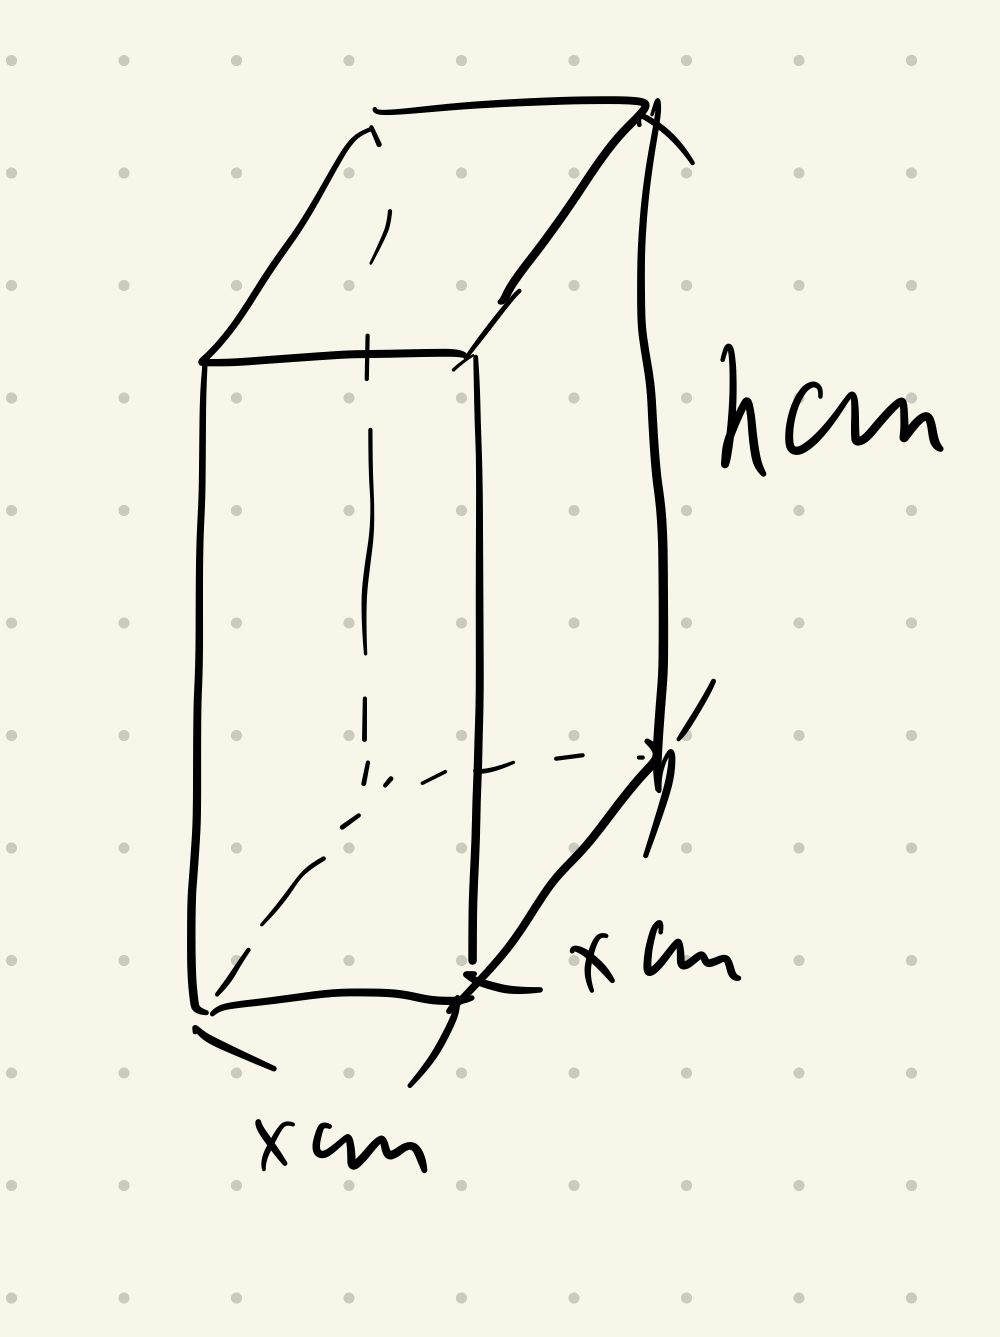
\includegraphics[width = 0.25\textwidth]{figures/chap 05/optimization_box.png}
        \label{fig: ex_optimization_box}
    \end{center}
    Suppose the box has the dimensions above, then we have, from the surface area of the box:
    \[x^2+4xh = 300\]
    Solving for $h$ with $x$ leads us to
    \[h = \frac{300-x^2}{4x}\]
    Therefore, the volume of the box (in cm$^3$), which we are aiming to maximize, is
    \[V := x^2h = x^2\frac{300-x^2}{4x} = 75x-\frac{1}{4}x^3\]
    Note that the possible values of $x$ are restricted by the facts that (1) $x$ refers to the length of the sides for the base, so $x > 0$ (2) $h$ refers to the height of the box, so $h > 0$. $h > 0$ implies that
    \[\frac{300-x^2}{4x} > 0\]
    \[(300-x^2)(4x) > 0\]
    \[(x^2-300)x < 0\]
    \[(x+10\sqrt{3})x(x-10\sqrt{3}) < 0\]
    \[x < -10\sqrt{3} \text{ or } 0 < x < 10\sqrt{3}\]
    Combined with $x > 0$, we have our range of input $x \in (0,10\sqrt{3})$.  To find the global maximum of the volume $V(x) = 75x - \frac{1}{4}x^3$ (which is a continuous function) within $x \in (0, 10\sqrt{3})$, we first find its critical points.  The first derivative of $V(x)$ with respect to $x$ is 
    \[V'(x) = 75 - \frac{3}{4}x^2\]
    Since the first derivative always exists, we find the critical points that make $V'(x) = 0$, which leads to
    \[75-\frac{3}{4}x^2 = 0 \Rightarrow x^2 = 100 \Rightarrow x = \pm 10\]
    Since $x = -10$ is out of the domain $(0, 10\sqrt{3})$, the only critical point is $x = 10$.
    
    To determine if the function is attaining maximum, minimum or neither at $x = 10$, we can use the first derivative test and find that $V'(x) = 75 - \frac{3}{4}x^2$ is positive when $x$ is in $(0, 10)$ and negative when $x$ is in $(10, 10\sqrt{3})$.  Therefore, the volume is attaining both local maximum and global maximum at $x = 10$, with value $V(10) = 500$ (cm$^3$).
    \begin{center}
        \begin{tabular}{cccccc}
            $x$    & $0$ &   & $10$ &   & $10\sqrt{3}$  \\
            \hline
            $V'(x)$ &     & + &      & - & 
        \end{tabular}
    \end{center}
    Another way to show that global maximum is attained at $x = 10$ is to use the second derivative test.  Since $V''(x) = -\frac{3}{2}x$ is always negative in $(0, 10\sqrt{3})$, the function is always concaving down within the range of input, so the critical point $x = 10$ with $V'(x) = 0$ attains both local maximum and global maximum.
\end{egsol}

Note that in the previous example, since the interval of input is an open interval, we cannot verify that $x = 10$ attains global maximum by comparing its function value with the function values at the boundaries as we previously did.  Therefore, we resort to investigating the behavior of the first or second derivative to check the property of the function at $x = 10$.

\begin{ex}[]{ex: optimization_print}
    A poster with a total area of $200$ in$^2$ and has $1$ inch margins on the sides, a $2.5$-inch margin on the top and a $1.5$-inch margin on the bottom. What dimensions will give the largest printed area?
\end{ex}

\begin{exsol}[]{exsol: optimization_print}
    \begin{center}
        \includegraphicsex{width = 0.35\textwidth, draft}{width = 0.35\textwidth}{figures/chap 05/optimization_print.png}
        \label{fig: ex_optimization_print}
    \end{center}
    Suppose the poster is of the dimension as above, then from the total area of the poster, we have
    \[xy = 200 \qquad \Rightarrow \qquad y = \frac{200}{x}\]
    Therefore, the area of the printed area, which we are aiming to maximize, is
    \[A := (x-2)(y-4) = (x-2)\Big(\frac{200}{x}-4\Big) = 200-4x-\frac{400}{x}+8 = 208 - 4x - \frac{400}{x}\]
    Note that the possible values of $x$ are restricted that
    \begin{enumerate}
        \item the width of the printed area must be greater than zero, i.e. $x-2 > 0 \Rightarrow x > 2$
        \item the height of the printed area must be greater than zero, i.e. $y-4 > 0 \Rightarrow \frac{200}{x}>4 \Rightarrow 0 < x < 50$
        \item both $x$ and $y$ stand for lengths, so $x > 0$ and $y > 0 \Rightarrow x > 0$.  
    \end{enumerate}
    
    Combining the above and we yield the range of input for $x$: $(2, 50)$.  To find the global maximum of the volume $A(x) = 208-4x-\frac{400}{x}$ (which is a continuous function) within $x \in (2, 50)$, we first find its critical points.  The first derivative of $A(x)$ with respect to $x$ is 
    \[A'(x) = -4 + \frac{400}{x^2}\]
    Although $A'(x)$ does not exist when $x=0$, this point is not within $(2, 50)$, so it is not a critical point.  We then find the critical points that make $A'(x) = 0$, which leads to
    \[-4 +\frac{400}{x^2} = 0 \Rightarrow x^2 = 100 \Rightarrow x = \pm 10\]
    Since $x = -10$ is out of $(2, 50)$, the only critical point is $x = 10$.
    
    To determine if the function is attaining maximum, minimum or neither at $x = 10$, we use the first derivative test and find that $A'(x) = -4 + \frac{400}{x^2}$ is positive when $x$ is in $(2, 10)$ and negative when $x$ is in $(10, 50)$.  Therefore, the volume is attaining both local maximum and global maximum at $x = 10$, with value $A(10) = 208-40-40 = 128$ (in$^2$).
    \begin{center}
        \begin{tabular}{cccccc}
            $x$    & $2$ &   & $10$ &   & $50$  \\
            \hline
            $A'(x)$ &     & + &      & - & 
        \end{tabular}
    \end{center}
    Another way to show that global maximum is attained at $x = 10$ is to use the second derivative test.  Since $AV''(x) = -\frac{800}{x^3}$ is always negative in $(2, 50)$, the function is always concaving down within the range of input, so the critical point $x = 10$ with $A'(x) = 0$ attains both local maximum and global maximum.
\end{exsol}

\begin{ex}[]{ex: AM-GM}
    Prove the arithmetic mean-geometric mean (AM-GM) inequality: Suppose $x$ and $y$ are both positive, then $\frac{x+y}{2} \ge \sqrt{xy}$, where the equality is attained when $x = y$.
\end{ex}

\begin{exsol}[]{exsol: AM-GM}
    We now try to show that if denote $A := xy$, then $\frac{x+y}{2}$ has a global minimum at $x = y = \sqrt{A}$ with value $\sqrt{A} = \sqrt{xy}$.  Expressing $y$ with $A$ and $x$ and we yield $y = \frac{A}{x}$, and the function we are trying to minimize is $f(x) = \frac{x+A/x}{2}$.  The range of input for $x$ must guarantee (1) $x$ is positive, i.e. $x > 0$ (2) $y$ is positive, i.e. $y = \frac{A}{x} > 0 \Rightarrow x > 0$.  So the combined restriction of input is $x \in (0, \infty)$.
    
    To find the global maximum of the volume $f(x) = \frac{x+A/x}{2}$ (which is a continuous function) within $x \in (0, \infty)$, we first find its critical points.  The first derivative of $f(x)$ with respect to $x$ is 
    \[f'(x) = \frac{1}{2} - \frac{A}{2x^2}\]
    Although $f'(x)$ does not exist when $x=0$, this point is not within $(0, \infty)$, so it is not a critical point.  We then find the critical points that make $f'(x) = 0$, which leads to
    \[\frac{1}{2} - \frac{A}{2x^2} = 0 \Rightarrow x^2 = A \Rightarrow x = \pm \sqrt{A}\]
    Since $x = -\sqrt{A}$ is out of $(0, \infty)$, the only critical point is $x = \sqrt{A}$.
    
    To determine if the function is attaining maximum, minimum or neither at $x = \sqrt{A}$, we use the first derivative test and find that $f'(x) = \frac{1}{2} - \frac{A}{2x^2}$ is negative when $x$ is in $(0, \sqrt{A})$ and positive when $x$ is in $(\sqrt{A}, \infty)$.  Therefore, the function is attaining both local minimum and global minimum at $x = \sqrt{A}$, with value $f(\sqrt{A}) = \sqrt{A}$.
    
    \begin{center}
        \begin{tabular}{ccccc}
            $x$    & $0$ &   & $\sqrt{A}$ &     \\
            \hline
            $f'(x)$ &     & - &      & +
        \end{tabular}
    \end{center}
    
    Therefore, the minimum value $\frac{x+y}{2}$ can attain is $\sqrt{xy}$, where it is attained at $x = y = \sqrt{xy}$.
\end{exsol}

% \chapter{Antiderivatives and Antidifferentiation Techniques}
% \section{Definition of Antiderivatives and the Mean Value Theorem}
In previous chapters, we have learned the derivatives of several common functions, and how to use a set of differentiation rules to find the derivatives of functions that are built from common functions.  We are now like wizards that are ever powerful.  Given any function, no matter how complicated they are, we can repeatedly use the set of rules to produce its derivative.  Now we turn our focus to finding \textit{antiderivatives}, which is the \textit{reverse} of finding derivatives.  Given an arbitrary function, we would like to know \textit{which function has it as the derivative}.  The process of finding antiderivatives is called \textit{antidifferentiation}.  For example, suppose we are given a function
\[f(x) = 4x^3\]
since we know that $\frac{d}{dx}x^4 = 4x^3 = f(x)$, we say that $F(x) = x^3$ is an \textit{antiderivative} for $f(x)$.  However, notice that $\frac{d}{dx}(x^4+1) = 4x^3 = f(x)$, so $G(x) = x^4+1$ is also an antiderivative for $f(x)$.  Now it seems that we are doomed: there are multiple functions that has the same derivative $4x^3$, so how can we be sure that we can find or have found all of them?  Fortunately, we have a very important theorem that can guide us through this mess.

\begin{theo}[Mean Value Theorem]{thm: MVT}
    Let $f(x)$ be a function that is continuous in $[a, b]$ and differentiable in $(a, b)$, then there exists $c$ in $(a, b)$ such that
    \[f'(c) = \frac{f(b)-f(a)}{b-a}\]
\end{theo}
This theorem can be better explained by the graph in the next page.  There are two points $A(a, f(a))$ and $B(b, f(b))$ on the curve of a differentiable function $f(x)$.  Then $\frac{f(b)-f(a)}{b-a}$ is the slope of the secant line shown in red.  What Mean Value Theorem tells us is that you can always find a point $C(c, f(c))$ on the curve between $A$ and $B$, such that the tangent line over $C$ has the same slope as the secant line, such as the blue line in the graph.  Though this theorem seems very intuitive, it can help us prove an essential lemma.

\begin{figure}[ht]
    \centering
    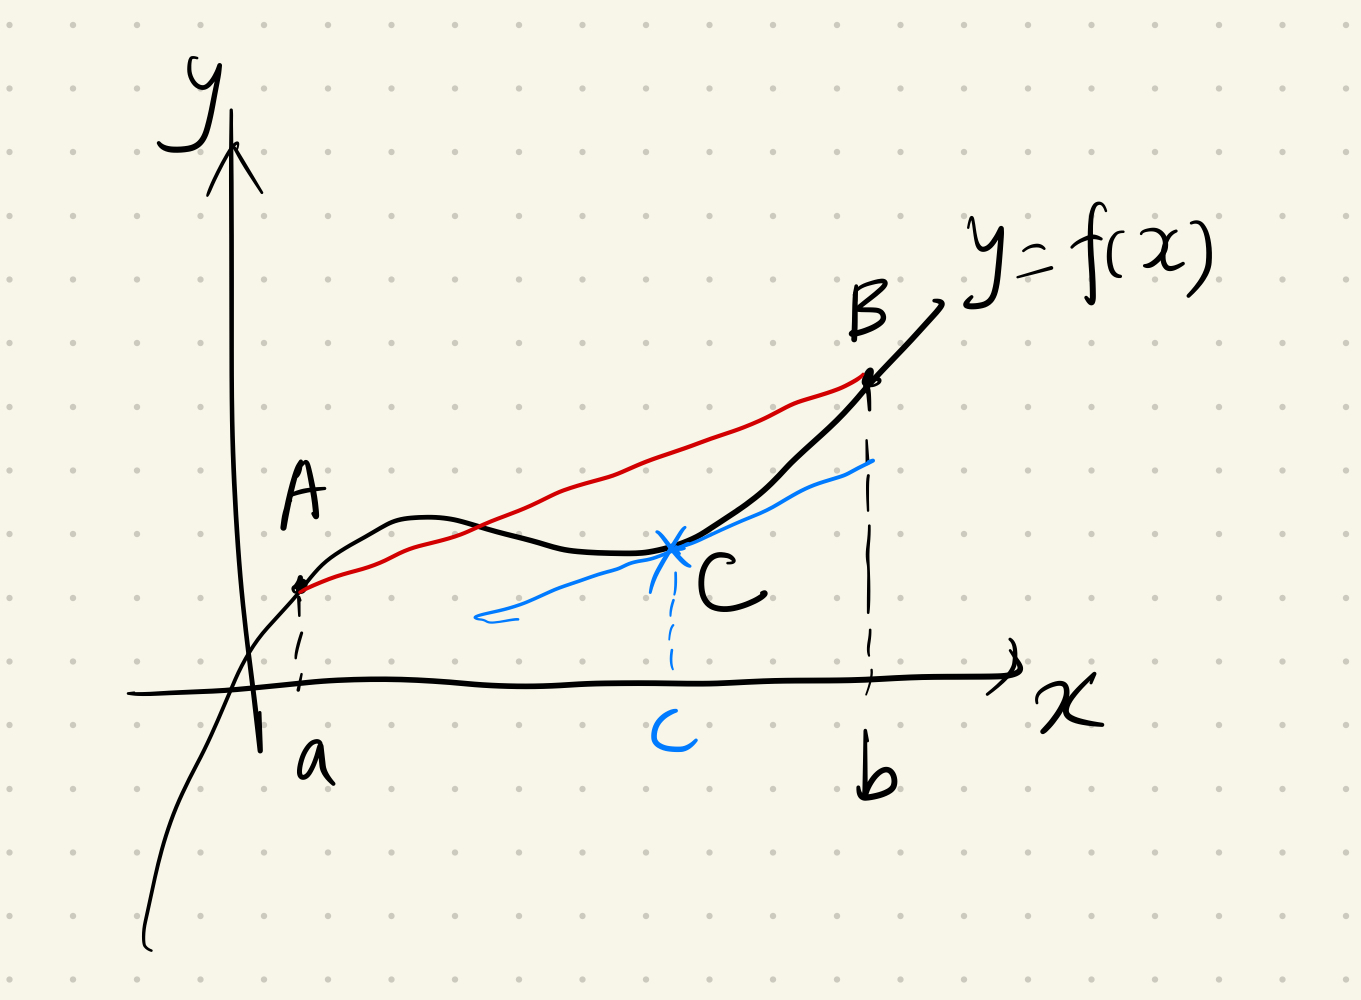
\includegraphics[width = 0.5\textwidth]{figures/chap 06/MVT.png}
\end{figure}

\newpage

\begin{lem}[The Antiderivative of Zero]{lem: zero_integral}
    If $f'(x) = 0$ within $(a,b)$, then $f(x) = C$ within $(a,b)$, where $C$ is a constant.
\end{lem}

\begin{prf}[]{pf: zero_integral}
    We use proof by contradiction.  
    
    Suppose $f'(x) = 0$ within $(a, b)$ but $f(x)$ is \textit{not} constant within $(a, b)$.  Then we can find two extra points $(c, f(c))$ and $(d, f(d))$ where $a < c < d < b$ and $f(c) \ne f(d)$.  
    
    Now we know that $f(x)$ is continuous within $[c, d]$ and differentiable within $(c, d)$ (because it is differentiable in $(a, b)$).  So by the Mean Value Theorem, there exists $t$ in $(c, d)$ such that $f'(t) = \frac{f(d)-f(c)}{d-c} \ne 0$, which contradicts the assumption that $f'(x) = 0$ within $(a, b)$.  Therefore, $f(x)$ must be a constant within $(a, b)$. 
\end{prf}

Now we can show the following theorem:

\begin{theo}[Constant of Integration]{thm: C_in_int}
    Suppose $F(x)$ and $G(x)$ are both antiderivatives for $f(x)$, then there exists a constant $C$ so that $G(x) = F(x) + C$.
\end{theo}

\begin{prf}[]{pf: C_in_int}
    We define $H(x) = G(x) - F(x)$.  Then we have $H'(x) = G'(x) - F'(x) = f(x) - f(x) = 0$.  From Lemma \ref{lem: zero_integral}, we thus know that $H(x) = C$ where $C$ is a constant.  Therefore $G(x) = F(x) + C$.
\end{prf}

Therefore, if $F(x)$ is \textit{one} of the antiderivatives for a function $f(x)$, then \textit{all} the antiderivatives for $f(x)$ would be shaped as $F(x) + C$, where $C$ is a unknown constant.  In other words, we only need to strive to find one antiderivative, then add $+C$ in the end and call it a day, without fearing that some other weird function would also be an antiderivative.  In the previous example, the antiderivative of $f(x) = 4x^3$ can then be written as $x^4 + C$.

In previous sections, we used $f'(x)$ or $\frac{d}{dx}f(x)$ to denote the derivative of $f(x)$.  For antiderivatives, we also have a notation written as
\[\int f(x) dx\]
where $\int$ is the integration sign, derived from a elongated "S" standing for summation.  We will talk about the link between antiderivatives and integrals in the next chapter, so up until now please bear with the name.  The function to be antidifferentiated, $f(x)$, is also called the \textit{integrand}.  $dx$ is a symbol that tells us that with respect to what variable are we antidifferentiating.  Later we will introduce its formal name: the \textit{differential}.  Using this new notation, we can now write
\[\int 4x^3 dx = x^4 + C\]
With these new concepts and notations at hand, let us look at some examples of antiderivatives:
\begin{eg}[]{eg: antiderivative}
    Find the following antiderivatives:
    \begin{tasks}(4)
        \task $\int 3 dx$
        \task $\int 2x dx$
        \task $\int 6x^5 dx$
        \task $\int -\frac{1}{x^2} dx$
        \task $\int \cos x dx$
        \task $\int -\sin x dx$
        \task $\int e^x dx$
        \task $\int \frac{1}{x} dx$
    \end{tasks}
\end{eg}

\begin{egsol}[]{egsol: antiderivative}
    \begin{enumerate}[a)]
        \item We know for any constant $k$
        \[\frac{d}{dx}kx = k\]
        so $3x$ is \textit{one} of the antiderivatives of $3$, and we have $\int 3 dx = 3x + C$.
        \item In the power rule for differentiation, we have 
        \[\frac{d}{dx} x^r = r x^{r-1}\]
        where the power decreases by $1$ after differentiation.  This prompts us to guess that the antiderivative for a multiple of $x^r$ should be a multiple of $x^{r+1}$, where the power increases by $1$ after antidifferentiation.  Here we can try guessing $x^2$ and verify that
        \[\frac{d}{dx} x^2 = 2x\]
        which gets to our desired function.  Therefore, $x^2$ is \textit{one} of the antiderivatives for $2x$ and we have $\int 2x dx = x^2 + C$.
        \item Similar to the previous subproblem, since $6x^5$ is a multiple of $x^5$, we can use the reverse of power rule and try guessing something like $x^6$ and verify that
        \[\frac{d}{dx} x^6 = 6x^5\]
        so we know $x^6$ is \textit{one} of the antiderivatives for $6x^5$, and we have $\int 6x^5 dx = x^6 + C$.
        \item Here $-\frac{1}{x^2}$ can actually be rewritten as $-x^{-2}$, so it is a multiple of power of $x$.  Therefore, we can try guessing $x^{-1}$ for its antiderivative and verify that
        \[\frac{d}{dx}x^{-1} = -x^{-2}\]
        so that $x^{-1}$ indeed an antiderivative for $-x^{-2}$.  Therefore we have $\int -\frac{1}{x^2} dx = -\frac{1}{x} + C$.
        \item We have known by heart that
        \[\frac{d}{dx}\sin x = \cos x\]
        so we already know $\sin x$ is \textit{one} of the antiderivatives for $\cos x$.  Therefore we have $\int \cos x dx = \sin x + C$.
        \item Likewise, we already know that 
        \[\frac{d}{dx}\cos x = -\sin x\]
        so $\cos x$ is \textit{one} of the antiderivatives for $-\sin x$, and we have $\int -\sin x dx = \cos x + C$.
        \item $e^x$ is a special function where 
        \[\frac{d}{dx} e^x = e^x\]
        therefore $e^x$ is an antiderivative for $e^x$ itself, so we have $\int e^x dx = e^x + C$.
        \item Recall than the derivative of $\ln x$
        \[\frac{d}{dx} \ln x = \frac{1}{x}\]
        therefore intuitively, we would say that $\ln x$ is an antiderivative for $\frac{1}{x}$.  However, this is just part of the answer.  Notice that when we differentiate $\ln x$ and get $1/x$, we are implicitly assuming that $x$ can only take up positive values in both functions, since $\ln x$ is defined only for $x > 0$.  However, when we are antidifferentiating $1/x$, since $1/x$ is defined for all non-zero real numbers, we would also want the resulting antiderivative to be defined for all non-zero real numbers.  This can be done by looking into the function $\ln |x|$.  Note that when $x > 0$:
        \[\frac{d}{dx} \ln |x| = \frac{d}{dx} \ln x = \frac{1}{x}\]
        and when $x < 0$:
        \[\frac{d}{dx} \ln |x| = \frac{d}{dx} \ln (-x) = \frac{1}{-x}(-1) = \frac{1}{x}\]
        therefore, $\ln |x|$ is indeed an antiderivative for $1/x$, and it is also defined for all non-zero real numbers.  In the end, we would write $\int \frac{1}{x} dx = \ln |x| + C$.
    \end{enumerate}
\end{egsol}

\bigskip

Eminent students may argue that $\ln |x| + C$ does not actually cover all possible antiderivatives for $\frac{1}{x}$, since the following function also has derivative $\frac{1}{x}$:
\[F(x) = \begin{cases} \ln |x| + C_1, x > 0 \\ \ln |x| + C_2, x < 0 \end{cases}\]
Indeed, the "$+C$" trick breaks down here.  This is because when we were proving Theorem 6.3, the argument that $G'(x) - F'(x) = f(x) - f(x) = 0$ is only valid if $f(x)$ exists everywhere, while here $1/x$ is undefined at $x = 0$.  However, in this course we acknowledge that this weakness exists and continue to use $\ln |x| + C$ for simplicity.

\bigskip

\begin{ex}[]{ex: antiderivative}
    Find the following antiderivatives:
    \begin{tasks}(4)
        \task $\int 0~dx$
        \task $\int dx$
        \task $\int 2dt$
        \task $\int \frac{1}{2\sqrt{x}} dx$
        \task $\int \frac{2}{3\sqrt[3]{x}} dx$
        \task $\int \frac{1}{1+x^2} dx$
        \task $\int 2^x \ln 2~dx$
        \task $\int \sec^2 x dx$
    \end{tasks}
\end{ex}

\begin{exsol}[]{exsol: antiderivative}
    \begin{enumerate}[a)]
        \item In Lemma 6.2, we showed that the antiderivative of $0$ is a constant function $C$, so $\int 0~dx = C$.
        \item Here $\int dx$ is the shorthand of $\int 1 dx$.  Based on previous observations, we would guess and verify that $x$ is one antiderivative for $1$.  Therefore we have $\int dx = x + C$.
        \item Notice that here we are antidifferentiating with respect to $t$ instead of $x$, since the differential is $dt$ instead of $dx$.  Based on previous observations, we would guess and verify that $2t$ is one antiderivative for $2$.  Therefore we have $\int 2dt = 2t + C$.
        \item Here $\frac{1}{2\sqrt{x}}$ can be rewritten as $\frac{1}{2}x^{-1/2}$, which is a multiple of $x^{-1/2}$, a power function of $x$.  Therefore, we would naturally guess $x^{-1/2 + 1} = x^{1/2} = \sqrt{x}$ to be one of its antiderivatives, which checks out.  Therefore we have $\int \frac{1}{2\sqrt{x}} dx =  \sqrt{x} + C$
        \item Here $\frac{2}{3\sqrt[3]{x}}$ can be rewritten as $\frac{2}{3}x^{-1/3}$, which is a multiple of $x^{-1/3}$, a power function of $x$.  Therefore, we would naturally guess $x^{-1/3 + 1} = x^{2/3} = \sqrt[3]{x^2}$ to be one of its antiderivatives, which checks out.  Therefore we have $\int \frac{2}{3\sqrt[3]{x}} dx = \sqrt[3]{x^2} + C$.
        \item We specifically derived the derivatives of inverse trigonometic functions in Chapter 4, where we had the identity
        \[\frac{d}{dx}\arctan x = \frac{1}{1+x^2}\]
        Therefore, $\arctan x$ is one of the antiderivatives for $\frac{1}{1+x^2}$, and we have $\int \frac{1}{1+x^2} dx = \arctan x + C$.
        \item In the section where we talked about derivatives of exponential functions, we had the identity
        \[\frac{d}{dx} a^x = a^x \ln a, \quad \forall a > 0\]
        Therefore, $2^x$ is one of the antiderivatives for $2^x \ln 2$, and we have $\int 2^x \ln 2~dx = 2^x + C$.
        \item If you have memorized this one, you would immediately think of the identity
        \[\frac{d}{dx} \tan x = \sec^2 x\]
        Therefore, $\tan x$ is one of the antiderivatives for $\sec^2 x$, and we have $\int \sec^2 xdx = \tan x + C$.
    \end{enumerate}
\end{exsol}

\newpage
Like differentiation, we also have a set of basic antidifferentiation rules that can aid us in finding antiderivatives, which we list below:

\begin{itemize}
    \item Constant rule:
    \[\int k dx = kx + C, \quad \text{where }k\text{ is a constant}\]
    \item Power rule:
    \[\int x^r dx = \frac{1}{r+1}x^{r+1} + C, r \ne -1\]
    \item Constant multiplication rule:
    \[\int kf(x) dx = k\int f(x) dx, \quad \text{where }k\text{ is a constant}\]
    \item Sum and difference rule:
    \[\int f(x) \pm g(x) dx = \int f(x) dx \pm \int g(x) dx\]
\end{itemize}

We can put these rules to the test in the following example.

\bigskip

\begin{eg}[]{eg: antiderivative_rules}
    Find the following antiderivatives.
    \begin{tasks}(4)
        \task $\int 7x dx$
        \task $\int \frac{5}{x^4} dx$
        \task $\int \sqrt{x} dx$
        \task $\int (x^3 - 4x^2 + 3) dx$
        \task $\int (x+1)(x-3) dx$
        \task $\int \frac{2x + 1}{\sqrt{x}} dx$
        \task $\int \frac{2+\sqrt[5]{x}}{x} dx$ 
        \task $\int (x\sqrt{x} + 3\sin x) dx$
    \end{tasks}
\end{eg}

\begin{egsol}[]{egsol: antiderivative_rules}
    \begin{enumerate}[a)]
        \item Using the constant multiplication and power rule, we have
        \[\int 7x dx = 7 \int x^1 dx = 7 \Big(\frac{1}{1+1}x^{1+1} + C_1\Big) = \frac{7}{2}x^2 + C\]  Note that here $C_1$ is the constant term generated by antidifferentiating $\int x dx$, and in the end we let $C = 7C_1$ to be the new constant for aesthetic purpose.  It is perfectly valid to leave it like $\frac{7}{2}x^2 + 7C_1$, since it still implies that we need to add an unknown constant to $\frac{7}{2}x^2$.  In future derivations, sometimes we will skip these nuances and write $C$ directly as long as it is not confusing.
        \item Using the constant multiplication and power rule, we have
        \[\int \frac{5}{x^4} dx = 5\int x^{-4} dx = 5 \Big(\frac{1}{-4+1} x^{-4+1} dx\Big) = 5\cdot\frac{1}{-3} x^{-3} + C = -\frac{5}{3x^3} + C\]
        \item Writing $\sqrt{x}$ as $x^{1/2}$ and using the power rule, we have
        \[\int \sqrt{x} dx = \int x^{1/2} dx = \frac{1}{1/2+1}x^{1/2+1} + C = \frac{2}{3}x^{3/2} + C= \frac{2}{3}\sqrt{x^3} + C\]
        \item Using the power, constant and sum rule, we have
        \begin{align*}
            \int (x^3 - 4x^2 + 3) dx &= \int x^3 dx - 4 \int x^2 dx + \int 3~dx\\
            &= \Big(\frac{1}{3+1} x^{3+1}\Big) + C_1 - 4 \Big(\frac{1}{2+1}x^{2+1} + C_2\Big) + \Big(3x + C_3\Big)\\
            &= \frac{1}{4}x^4 - \frac{4}{3}x^3 + 3x + C
        \end{align*}
        Here notice that we let $C = C_1 - 4C_2 + C_3$ to simplify the constants.
        \item Though it is enticing to look for some kind of product rule, there is none for antidifferentiation.  We will have to expand the product and yield:
        \begin{align*}
            \int (x+1)(x-3) dx &= \int (x^2-2x-3) dx\\
            &= \frac{1}{2+1}x^{2+1} - 2 \cdot \frac{1}{1+1}x^{1+1} - 3x + C\\
            &= \frac{1}{3}x^3 - x^2 - 3x + C
        \end{align*}
        Note that here we avoided the fuss of having a bunch of constants by writing $C$ directly.
        \item It is also enticing here to try and find some kind of quotient rule, which is also non-existent for antidifferentiation.  Here we have to divide out the fraction and yield
        \begin{align*}
            \int \frac{2x + 1}{\sqrt{x}} dx &= \int \Big(\frac{2x}{\sqrt{x}} + \frac{1}{\sqrt{x}}\Big) dx\\
            &= \int \Big(2x^{1/2} + x^{-1/2}\Big) dx\\
            &= 2\cdot\frac{1}{1+1/2}x^{1/2+1} + \frac{1}{1+(-1/2)}x^{1+(-1/2)} + C\\
            &= \frac{4}{3}x^{3/2} + 2x^{1/2} + C\\
            &= \frac{4}{3}\sqrt{x^3} + 2\sqrt{x} + C
        \end{align*}
        \item We will divide out the fraction and yield
        \begin{align*}
            \int \frac{2+\sqrt[5]{x}}{x} dx &= \int \Big(\frac{2}{x} + \frac{\sqrt[5]{x}}{x}\Big) dx\\
            &= \int \Big(2 \cdot \frac{1}{x} + x^{-4/5}\Big) dx\\
            &= 2 \ln |x| + \frac{1}{-4/5 + 1} x^{-4/5 + 1} + C\\
            &= 2 \ln |x| + 5x^{1/5} + C\\
            &= 2 \ln |x| + 5\sqrt[5]{x} + C
        \end{align*}
        Notice that the antiderivative $\ln |x|$ we deduced previously appears again here.  Do not misuse the power rule for the antiderivative of $1/x$!
        \item Previously we have argued that the antiderivative of $-\sin x$ is $\cos x + C$, so we can write
        \begin{align*}
            \int (x\sqrt{x} + 3\sin x) dx &= \int [x^{3/2}+ (-3) (-\sin x)]dx\\
            &= \frac{1}{3/2+1} x^{3/2+1} - 3 \cos x + C\\
            &= \frac{2}{5}x^{5/2} - 3 \cos x + C\\
            &= \frac{2}{5}\sqrt{x^5} - 3 \cos x + C
        \end{align*}
    \end{enumerate}
\end{egsol}

\newpage
\begin{ex}[]{ex: antiderivative_rules}
    Find the following antiderivatives.
    \begin{tasks}(4)
        \task $\int (x+1)^3 dx$
        \task $\int \sqrt[3]{2x} dx$
        \task $\int 3^x dx$
        \task $\int (3\sin x + 5\cos x) dx$
        \task $\int e^{x+2} dx$
        \task $\int \frac{x^2}{1+x^2} dx$
        \task $\int \cos^2 \frac{x}{2} dx$ 
        \task $\int \tan^2 x dx$
    \end{tasks}
\end{ex}

\begin{exsol}[]{exsol: antiderivative_rules}
    \begin{enumerate}[a)]
        \item Here our tools are limited, and we can only expand the polynomial and yield:
        \begin{align*}
            \int (x+1)^3 dx &= \int (x^3 + 3x^2 + 3x + 1) dx \\
            &= \frac{1}{4} x^4 + 3\cdot\frac{1}{3} x^3 + 3\cdot\frac{1}{2}x^2 + x + C\\
            &= \frac{1}{4} x^4 + x^3 + \frac{3}{2}x^2 + x + C
        \end{align*}
        \item We can rewrite the function to pull the constant out and yield
        \[\int \sqrt[3]{2x} dx = \int (\sqrt[3]{2} \sqrt[3]{x}) dx = \int (\sqrt[3]{2} x^{1/3}) dx = \sqrt[3]{2} \cdot \frac{1}{4/3}x^{4/3} + C = \frac{3}{4}\sqrt[3]{2x^4} + C\]
        \item Previously we have shown that the antiderivative of $f(x) = 2^x \ln 2$ is $2^x + C$, therefore here we have
        \[\int 3^x dx = \int \Big(\frac{1}{\ln 3}3^x\ln 3\Big) dx = \frac{1}{\ln 3} 3^x + C\]
        \item Previously we have shown that the antiderivative of $f(x) = \cos x$ is $\sin x + C$, and the antiderivative of $g(x) = -\sin x$ is $\cos x + C$.  Therefore,
        \[\int (3\sin x + 5\cos x) dx = \int [(-3)(-\sin x) + 5\cos x] dx = -3\cos x + 5\sin x + C\]
        \item Given that the antiderivative of $f(x) = e^x$ is $e^x + C$, we may pull the $e^2$ out as constant muliplier and yield
        \[\int e^{x+2} dx = \int e^2e^x dx = e^2e^x + C = e^{x+2} + C\]
        \item Note that we already know the antiderivative of $f(x) = \frac{1}{1+x^2}$ is $\arctan x + C$, and the integrand can actually be written as $1-f(x)$.  Therefore,
        \[\int \frac{x^2}{1+x^2} dx = \int \Big(1-\frac{1}{1+x^2}\Big)dx = x - \arctan x + C\]
        \item Here we will use the identity that $\cos 2\alpha = 2\cos^2 \alpha - 1$.  Letting $\alpha = \frac{x}{2}$ then we get $\cos x = 2 \cos^2 \frac{x}{2} - 1$.  So we can rewrite the integrand and yield
        \[\int \cos^2 \frac{x}{2} dx = \int \frac{\cos x + 1}{2} dx = \int \Big(\frac{1}{2}\cos x + \frac{1}{2}\Big) = \frac{1}{2}\sin x + \frac{1}{2} x + C = \frac{x + \sin x}{2} + C\]
        \item We do not directly know the antiderivative of $\tan^2 x$, but note that $\tan^2 x + 1 = \sec^2 x$, and we have shown the antiderivative of $f(x) = \sec^2 x$ is $\tan x + C$.  Therefore, we can rewrite the integrand as,
        \[\int \tan^2 x dx = \int (\sec^2 x - 1) dx = \tan x - x + C\]
    \end{enumerate}
\end{exsol}

Up until now, we can see that at times our way of antidifferentiation requires some clever inspiration and even some guessing.  You may think that there should be a more extensive set of rules that enables us to antidifferentiate all kinds of functions.  Unfortunately, this is not the case.  In differentiation, with a function as ugly as 
\[f(x) = \sin\Big(\frac{\sqrt[3]{\ln(x)}}{e^{\arctan x}}\Big)\]
we can still find its derivative, albeit with some labor.  However, in antidifferentiation, even with a function as clean as
\[f(x) = \sin(x^2)\]
we \textit{cannot} find a closed form expression for its antiderivatives!  This shows how hard is it to find antiderivatives: even if we know a lot of antidifferentiation techniques, more often than not, we will still need a lot of luck to be able to antidifferentiate a random function.  

Nevertheless, we cannot give up here!  In the following, we will go over some of the antidifferentiation techniques that can increase our odds in finding antiderivatives of a function.

\newpage

\section{Antidifferentiation techniques: Variable substitution}
In the previous section, we could do some antidifferentiation with the simple rules provided, as long as the function to be antidifferentiated can be written as addition of functions of known antiderivatives.  However, for problems like
\[\int \frac{x}{\sqrt{x^2+1}} dx\]
our hands are tied.  Luckily, we have a technique in our arsenal that can solve some of the antidifferentiation problems of this kind.  Before we get into it, let us circle back and talk about differentials.

\subsection{Differentials}
In our notation for antidifferentiation, there is a mysterious notation "$dx$" that we termed as \textit{differentials}.  Previously in differentiation, we did not write $dx$ on its own, but only included it in the differentiation operate "$\frac{d}{dx}$".  However, we can reinspect the definition of derivatives, say $u$ is a function of $x$
\[u'(x) = \frac{du}{dx} = \lim_{\Delta x \rightarrow 0} \frac{u(x+\Delta x) - u(x)}{\Delta x} := \lim_{\Delta x \rightarrow 0} \frac{\Delta u}{\Delta x}\]
Along with the following graph, we can alternatively see $du$ and $dx$ as "changes in $u$ and $x$ from $(x, u(x))$ \textit{along the tangent line}", so that their quotient is exactly the derivative.  

\begin{figure}[ht]
    \centering
    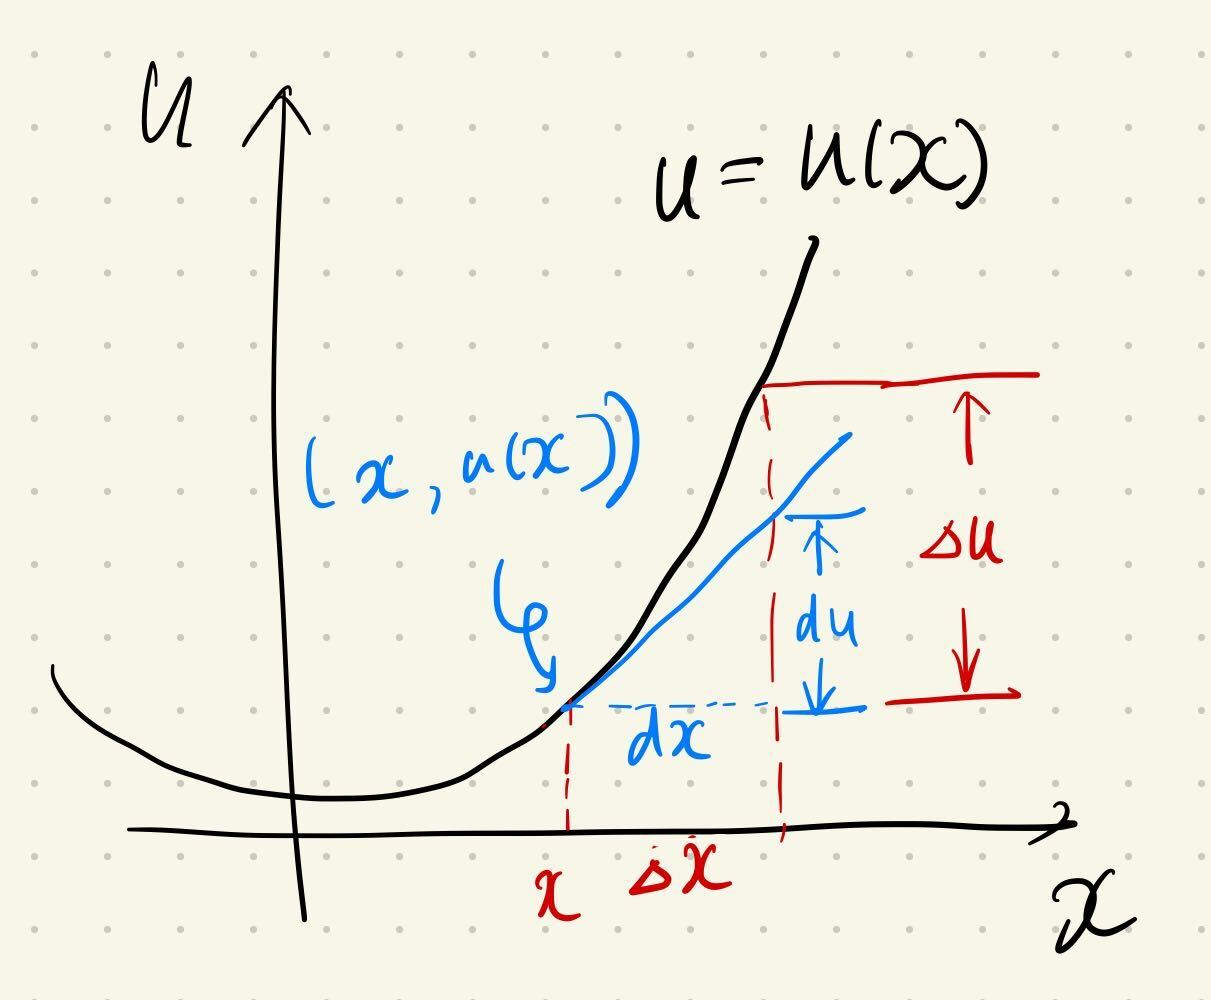
\includegraphics[width = 0.5\textwidth]{figures/chap 06/Differential.png}
\end{figure}

In this virtue, we can treat $du$ and $dx$ as manipulable entities and write
\[du = u'(x)dx\]
For example, say $u(x) = x^2$, then since $u'(x) = 2x$, we have $du = 2xdx$.  In fact, we have implicitly used the concept of differentials before when we we doing linear approximations.  Suppose we would like to approximate $u(x)$ around $x = x_0$, previously we used the tangent line equation and derived the linear approximant
\[\hat{u}(x) = u(x_0) + u'(x_0) (x - x_0)\]
Now with the differential notation, we can write $x = x_0 + dx$ and yield
\[\hat{u}(x) = \hat{u}(x_0 + dx) = u(x_0) + du = u(x_0) + u'(x_0)dx\]

To familiarize ourselves with the differential notation, let us look at a few examples:
\begin{eg}[]{eg: differentials}
    Given following functional relationship between $u$ and $x$, express $du$ with $dx$
    \begin{tasks}(4)
        \task $u = x + 1$
        \task $u = 3x + 2$
        \task $u = x^2 + 1$
        \task $u = \cos x$
        \task $u = x^3 - \sec x$
        \task $x = e^u$
        \task $x = \tan u$
        \task $x = \sin u$
    \end{tasks}
\end{eg}

\begin{egsol}[]{egsol: differentials}
    \begin{enumerate}[a)]
        \item Since $u'(x) = 1$, we have $du = u'(x)dx = dx$.
        \item Since $u'(x) = 3$, we have $du = u'(x)dx = 3dx$.
        \item Since $u'(x) = 2x$, we have $du = u'(x)dx = 2xdx$.
        \item Since $u'(x) = -\sin x$, we have $du = u'(x)dx = -\sin xdx$.
        \item Rewriting $u(x) = x^3 - \frac{1}{\cos x}$, we have $u'(x) = 3x^2 - \big(-\frac{1}{\cos^2 x}\big)\cdot(-\sin x) = 3x^2 - \tan x \sec x$.  Therefore, $du = u'(x)dx = (3x^2 - \tan x \sec x) dx$.
        \item Since $x'(u) = e^u$, we have $dx = x'(u)du = e^u du = x du$.  Therefore, $du = \frac{dx}{x}$.
        \item Since $x'(u) = \sec^2 u$, we have $dx = x'(u)du = \sec^2 u du = (1+\tan^2 u) du = (1+x^2) du$.  Therefore, $du = \frac{dx}{1+x^2}$.
        \item Since $x'(u) = \cos u$, we have $dx = x'(u)du = \cos u du$.  Therefore, $du = \frac{dx}{\cos u}$.  If $u$ is restricted between $-\frac{\pi}{2}$ and $\frac{\pi}{2}$, we can further reduce $\cos u = \sqrt{1-\sin^2 u} = \sqrt{1-x^2}$, so we have $du = \frac{dx}{\sqrt{1-x^2}}$.
    \end{enumerate}
\end{egsol}

\subsection{U-substitution}

Differentials are extremely useful in some types of antidifferentiation problems, since we can make the antidifferentiation tractable after replacing the variable of interest and substituting the differentials.  For example, in the teaser above where we try to fine $\int \frac{x}{\sqrt{x^2+1}} dx$, suppose we let $u = x^2 + 1$, then we have $du = 2xdx$, so we yield
\begin{align*}
    \int \frac{x}{\sqrt{x^2+1}} dx &= \int \frac{1}{2}\frac{2xdx}{\sqrt{x^2+1}}\\
    &= \int \frac{1}{2}\frac{du}{\sqrt{u}}\\
    &= \int \frac{1}{2} u^{-1/2} du\\
    &= \frac{1}{2} \cdot \frac{1}{1/2}u^{1/2} + C = \sqrt{u} + C = \sqrt{x^2+1} + C
\end{align*}
where we need to remember to substitute $u$ back to $x$.  We may check that this substitution trick is valid by differentiating $\sqrt{x^2+1} + C$ with respect to $x$, which gets us back to $\frac{x}{\sqrt{x^2+1}}$. 

This technique is called the \textbf{U-substitution} since in the midst of the derivation, we 
 substituted our original target of antidifferentiation, $x$, with a new variable $u$.  The general form of U-substitution can be written as follows:
\[\int f(u(x)) u'(x) dx = \int f(u) du = F(u) + C = F(u(x)) + C\]
where $F(.)$ is an antiderivative of $f(.)$.  In our example, we had $f(.)$ as the reciprocal of square root, and $u(x) = x^2 + 1$.

The million dollar question is whether we have a standard procedure that finds the appropriate $u(x)$ that makes U-substitution work.  Unfortunately, there isn't a one-size-fit-all solution, and sometimes we'll need some experience, quite a bit of trial and error, and a lot of luck.  However, we can reinspect what we have done above and come up with a general rule of thumb:
\begin{enumerate}
    \item We write out our antidifferentiation problem:
    \[\int \frac{x}{\sqrt{x^2+1}} dx\]
    \item First we inspect the integrand and find a portion in the integrand shaped like a composite function $f(u(x))$, where we \textit{know} the antiderivative of $f(.)$.  In the example above, $f(.)$ is the reciprocal of square root, and $u(x) = x^2 + 1$ is the function within $f(.)$.  
    \[\int \frac{\textcolor{blue}{x}}{\textcolor{red}{\sqrt{\textcolor{orange}{x^2+1}}}} dx = \int \textcolor{red}{\frac{1}{\sqrt{\textcolor{orange}{u}}}} \cdot \textcolor{blue}{x}dx\]
    Up until now we are doing the same thing as chain rule in derivatives, where we also trid to identify composite functions $f(u(x))$ that we know the derivative of $f(.)$.
    \item Right now in the integrand we have a function of $u$ and a remainder of function of $x$. Our goal is that after substituting the differential $dx$ with $du$, the function of $x$ would vanish, leaving us a pure integrand consisting of $u$.  Since $du = u'(x)dx$, the second step is to calculate $u'(x)$ and check that after dividing $u'(x)$ from the remainder of the integrand, \textit{there is no more $x$ left}.  If not, then we will have to go back to the previous step and pick a better $f(u(x))$. In the example above, $u'(x) = (x^2 + 1)' = 2x$, and the remainder of the integrand is $x$, so we have $\frac{x}{2x} = \frac{1}{2}$, which is free of $x$ and greenlights our U-substitution.
    \[\int \textcolor{red}{\frac{1}{\sqrt{\textcolor{orange}{u}}}} \cdot \textcolor{blue}{x} dx = \int \textcolor{red}{\frac{1}{\sqrt{\textcolor{orange}{u}}}} \cdot \textcolor{blue}{x} \textcolor{orange}{\frac{du}{u'(x)}} =\int \textcolor{red}{\frac{1}{\sqrt{\textcolor{orange}{u}}}} \cdot \underbrace{\frac{\textcolor{blue}{x}}{\textcolor{orange}{u'(x)}}}_{\substack{\text{Should not} \\ \text{depend on }x}} \textcolor{orange}{du}\]
    \item After confirming U-substitution may work, perform U-substitution based on the selected $f(.)$ and $u(x)$.
\end{enumerate}

In the following, let's look at some examples utilizing U-substitution.

\begin{eg}[]{eg: u_sub_1}
    Find the following antiderivatives.
    \begin{tasks}(4)
        \task $\int 2x(x^2+1)^3 dx$
        \task $\int 3x^2\sqrt{x^3-2} dx$
        \task $\int x\sqrt[3]{3-4x^2} dx$
        \task $\int \sqrt{1-5x} dx$
        \task $\int \frac{x}{1+4x^2} dx$
        \task $\int xe^{x^2+1} dx$
        \task $\int e^{2x}\sqrt{e^{2x}+1} dx$
        \task $\int x\sin(x^2) dx$ 
    \end{tasks}
\end{eg}

\begin{egsol}[]{egsol: u_sub_1}
    \begin{enumerate}[a)]
        \item The composite function here is pretty straightforward: $x^2+1$ as a whole is raised to the third power, so we may try $f(t) = t^3$ and $u(x) = x^2+1$.  Now since $u'(x) = 2x$ and the remainder of the integrand is $2x$, we have $\frac{2x}{2x} = 1$ which is independent of $x$, meaning that U-substitution may work.  We then have, letting $u = x^2+1$ and thus $du = 2xdx$:
        \begin{align*}
            \int 2x(x^2+1)^3 dx &= \int (x^2+1)^3 2xdx\\
            &= \int u^3 du\\
            &= \frac{1}{4}u^4 + C = \frac{1}{4}(x^2+1)^4 + C
        \end{align*}
        Remember the integration constant and substitution of $u$ back into terms of $x$.
        \item The composite function here looks like $x^3-2$ as a whole taken the square root, so we may try $f(t) = \sqrt{t}$ and $u(x) = x^3 - 2$.  Now since $u'(x) = 3x^2$ and the remainder of the integrand is $3x^2$, we have $\frac{3x^2}{3x^2} = 1$ which is independent of $x$.  We then have, letting $u = x^3 - 2$ and thus $du = 3x^2dx$:
        \begin{align*}
            \int 3x^2\sqrt{x^3-2} dx &= \int (x^3-2)^{1/2} 3x^2dx\\
            &= \int u^{1/2} du\\
            &= \frac{1}{1+1/2}u^{1+1/2} + C = \frac{2}{3}(x^3-2)^{3/2} + C
        \end{align*}
        \item The composite function here looks like $3-4x^2$ as a whole taken the cube root, so we may try $f(t) = \sqrt[3]{t}$ and $u(x) = 3 - 4x^2$.  Now since $u'(x) = -8x$ and the remainder of the integrand is $x$, we have $\frac{x}{-8x} = -\frac{1}{8}$ which is independent of $x$.  We then have, letting $u = 3 - 4x^2$ and thus $du = -8xdx$:
        \begin{align*}
            \int x\sqrt[3]{3-4x^2} dx &= -\frac{1}{8}\int (3-4x^2)^{1/3} (-8x)dx\\
            &= -\frac{1}{8}\int u^{1/3} du\\
            &= -\frac{1}{8}\cdot\frac{1}{1+1/3}u^{1+1/3} + C \\
            &= -\frac{1}{8}\cdot\frac{3}{4}u^{4/3} + C = -\frac{3}{32}(3-4x^2)^{4/3} + C
        \end{align*}
        Note that here after substituting the differentials, we yield an additional factor $-\frac{1}{8}$.
        \item The composite function here looks like $1-5x$ as a whole taken the square root, so we may try $f(t) = \sqrt{t}$ and $u(x) = 1-5x$.  Now since $u'(x) = -5$ and the remainder of the integrand is $1$, we have $\frac{1}{-5} = -\frac{1}{5}$ which is independent of $x$.  We then have, letting $u = 1-5x$ and thus $du = -5dx$:
        \begin{align*}
            \int \sqrt{1-5x} dx &= -\frac{1}{5}\int (1-5x)^{1/2} (-5)dx\\
            &= -\frac{1}{5}\int u^{1/2} du\\
            &= -\frac{1}{5}\cdot\frac{1}{1+1/2}u^{1+1/2} + C \\
            &= -\frac{1}{5}\cdot\frac{2}{3}u^{3/2} + C = -\frac{2}{15}(1-5x)^{3/2} + C
        \end{align*}
        \item The composite function here looks like $1+4x^2$ as a whole taken the reciprocal, so we may try $f(t) = \frac{1}{t}$ and $u(x) = 1+4x^2$.  Now since $u'(x) = 8x$ and the remainder of the integrand is $x$, we have $\frac{x}{8x} = \frac{1}{8}$ which is independent of $x$.  We then have, letting $u = 1+4x^2$ and thus $du = 8xdx$:
        \begin{align*}
            \int \frac{x}{1+4x^2} dx &= \frac{1}{8}\int  \frac{1}{1+4x^2} 8xdx\\
            &= \frac{1}{8}\int \frac{1}{u} du\\
            &= \frac{1}{8}\ln |u| + C = \frac{1}{8} \ln |1+4x^2| + C
        \end{align*}
        \item The composite function here looks like $x^2+1$ as a whole taken the exponential, so we may try $f(t) = e^t$ and $u(x) = x^2+1$.  Now since $u'(x) = 2x$ and the remainder of the integrand is $x$, we have $\frac{x}{2x} = \frac{1}{2}$ which is independent of $x$.  We then have, letting $u = x^2 + 1$ and thus $du = 2xdx$:
        \begin{align*}
            \int xe^{x^2+1} dx &= \frac{1}{2}\int e^{x^2+1} 2xdx\\
            &= \frac{1}{2}\int e^u du\\
            &= \frac{1}{2} e^u + C = \frac{1}{2} e^{x^2+1} + C
        \end{align*}
        \item The composite function here looks like $e^{2x}+1$ as a whole taken the square root, so we may try $f(t) = \sqrt{t}$ and $u(x) = e^{2x}+1$.  Now since $u'(x) = 2e^{2x}$ and the remainder of the integrand is $e^{2x}$, we have $\frac{e^{2x}}{2e^{2x}} = \frac{1}{2}$ which is independent of $x$.  We then have, letting $u = e^{2x} + 1$ and thus $du = 2e^{2x}dx$:
        \begin{align*}
            \int e^{2x}\sqrt{e^{2x}+1} dx &= \frac{1}{2}\int (e^{2x}+1)^{1/2} 2e^{2x}dx\\
            &= \frac{1}{2}\int u^{1/2} du\\
            &= \frac{1}{2}\cdot\frac{1}{1+1/2} u^{1+1/2} \\
            &= \frac{1}{2}\cdot\frac{2}{3} u^{3/2} + C = \frac{1}{3} (e^{2x}+1)^{3/2} + C
        \end{align*}
        \item The composite function here looks like $x^2$ as a whole taken the sine function, so we may try $f(t) = \sin t$ and $u(x) = x^2$.  Now since $u'(x) = 2x$ and the remainder of the integrand is $x$, we have $\frac{x}{2x} = \frac{1}{2}$ which is independent of $x$.  We then have, letting $u = x^2$ and thus $du = 2xdx$:
        \begin{align*}
            \int x \sin(x^2) dx &= \frac{1}{2}\int \sin(x^2) 2xdx\\
            &= \frac{1}{2}\int \sin u du\\
            &= \frac{1}{2} (-\cos u) + C = -\frac{1}{2} \cos(x^2) + C
        \end{align*}
    \end{enumerate}
\end{egsol}

\begin{ex}[]{ex: u_sub_1}
    Find the following antiderivatives.
    \begin{tasks}(3)
        \task $\int (1-\frac{1}{x}) \cos (x - \ln x) dx$
        \task $\int \sin x \cos x dx$
        \task $\int \sin(2x) (1 - \cos(2x))^3 dx$
        \task $\int \frac{2}{3x + 1} dx$
        \task $\int \frac{2x}{3x^2 + 1} dx$
        \task $\int \frac{2}{3x^2 + 1} dx$
        \task $\int \frac{x^2 + 1}{x^3 + 3x} dx$
        \task $\int \frac{x}{\sqrt{1-x^2}} dx$ 
        \task $\int \tan x dx$ 
    \end{tasks}
\end{ex}

 \begin{exsol}[]{exsol: u_sub_1}
    \begin{enumerate}[a)]
        \item The composite function here is pretty straightforward: $x - \ln x$ as a whole is taken the cosine function, so we may try $f(t) = \cos t$ and $u(x) = x - \ln x$.  Now since $u'(x) = 1 - \frac{1}{x}$ and the remainder of the integrand is exactly the same, we conclude that U-substitution may work.  We then have, letting $u = x - \ln x$ and thus $du = \big(1-\frac{1}{x}\big)dx$:
        \begin{align*}
            \int \Big(1-\frac{1}{x}\Big) \cos(x - \ln x) dx &= \int \cos(x - \ln x) \Big(1-\frac{1}{x}\Big)dx\\
            &= \int \cos u du\\
            &= \sin u + C = \sin(x - \ln x) + C
        \end{align*}
        \item Here we do not have an evident composite function, but we can let $f(t) = 1$ and $u(x) = \sin x$.  Then, the remaining integrand is $\cos x$, which is exactly $u'(x)$, so the U-substitution may work.  Letting $u = \sin x$ and thus $du = \cos x dx$ and we have:
        \[\int \sin x \cos x dx = \int u du = \frac{1}{2} u^2 + C = \frac{1}{2} \sin^2x + C\]
        Alternatively, we may let $u(x) = \cos x$ so that the remaining integrand is $\sin x$, which is equal to $-u'(x)$ so the U-substitution may still work.  Letting $u = \cos x$ and thus $du = -\sin x dx$ and we have:
        \[\int \sin x \cos x dx = -\int \cos x (-\sin x)dx = -\int u du = -\frac{1}{2} u^2 + C = -\frac{1}{2} \cos^2x + C\]
        Still another way is to recall that $\sin 2x = 2\sin x \cos x$, so we have, letting $u = 2x$ so that $du = 2dx$:
        \begin{align*}
            \int \sin x \cos x dx &= \frac{1}{2}\int 2 \sin x \cos x dx\\
            &= \frac{1}{2} \int \sin(2x) dx\\
            &= \frac{1}{4} \int \sin(2x) \cdot 2dx\\
            &= \frac{1}{4} \int \sin u du = \frac{1}{4} (- \cos u) + C = -\frac{1}{4}\cos 2x + C
        \end{align*}
        At first glance, it seems that the three methods are giving us different answers.  However, we can use two identities, $\sin^2 x + \cos^2 x = 1$ and $\cos 2x = 2 \cos^2x - 1$ to show that
        \begin{gather*}
            \frac{1}{2}\sin^2x + C = \frac{1}{2}(1-\cos^2x) + C = -\frac{1}{2}\cos^2x + \Big(C+\frac{1}{2}\Big)\\
            -\frac{1}{4}\cos 2x + C  = -\frac{1}{4}(2 \cos^2 x - 1) + C = -\frac{1}{2}\cos^2x + \Big(C+\frac{1}{4}\Big)
        \end{gather*}
        Since $C$ is any constant, we may redefine $C$ for the first and third method, then their answers would match the $-\frac{1}{2}\cos^2x + C$ solution.  That is, these three answers are \textit{de facto} equivalent.
        \item Here if we just let $u(x) = 2x$, then it would work since we still don't have a quick idea on how to antidifferentiate $\sin u (1- \cos u)^3$.  However, we can try letting $f(t) = t^3$ and $u(x) = 1-\cos (2x)$.  Now since $u'(x) = 2\sin(2x)$, which is twice the remainder, $\sin (2x)$, the U-substitution should work now.  We then have, letting $u = 1-\cos (2x)$ and thus $du = 2\sin (2x)dx$
        \begin{align*}
            \int \sin(2x)(1-\cos(2x))^3 dx &= \frac{1}{2}\int (1-\cos(2x))^3 2\sin(2x) dx\\
            &= \frac{1}{2}\int u^3 du\\
            &= \frac{1}{2}\cdot\frac{1}{4}u^{4} + C = \frac{1}{8}(1-\cos (2x))^4 + C
        \end{align*}
        \item The composite function here looks like $3x+1$ as a whole taken the reciprocal, so we may try $f(t) = \frac{1}{t}$ and $u(x) = 3x+1$.  Now since $u'(x) = 3$ and the remainder of the integrand is $2$, we have $\frac{2}{3}$ is independent of $x$ and U-substitution should work.  We then have, letting $u = 3x+1$ and thus $du = 3dx$:
        \begin{align*}
            \int \frac{2}{3x+1} dx &= \frac{2}{3}\int \frac{1}{3x+1} 3dx\\
            &= \frac{2}{3}\int \frac{1}{u} du\\
            &= \frac{2}{3}\ln |u| + C = \frac{2}{3} \ln |3x+1| + C
        \end{align*}
        \item The composite function here looks like $3x^2 +1$ as a whole taken the reciprocal, so we may try $f(t) = \frac{1}{t}$ and $u(x) = 3x^2 + 1$.  Now since $u'(x) = 6x$ and the remainder of the integrand is $2x$, we have $\frac{2x}{6x} = \frac{1}{3}$ which is independent of $x$.  We then have, letting $u = 3x^2 + 1$ and thus $du = 6xdx$:
        \begin{align*}
            \int \frac{2x}{3x^2 + 1} dx &= \frac{1}{3}\int \frac{1}{3x^2 + 1} 6xdx\\
            &= \frac{1}{3}\int \frac{1}{u} du\\
            &= \frac{1}{3}\ln |u| + C = \frac{1}{3} \ln |3x^2 + 1| + C
        \end{align*}
        \item Here if we still let $f(t) = \frac{1}{t}$ and $u(x) = 3x^2+1$, we would fail since  $u'(x) = 6x$ and the remainder of the integrand is $2$, and we have $\frac{2}{6x} = \frac{1}{3x}$ which is dependent of $x$.  On closer inspection, we can rewrite the integrand as:
        \[\frac{2}{3x^2+1} = \frac{2}{(\sqrt{3}x)^2 + 1}\]
        The denominator now has the shape of $\frac{1}{1+t^2}$, which reminds us of the arctangent function.  Therefore, letting $f(t) = \frac{1}{1+t^2}$ and $u(x) = \sqrt{3}x$, we have $u'(x) = \sqrt{3}$ and the integrand remainder $2$ are both constants, so the U-substitution should work.  We then have, letting $u = \sqrt{3}x$ and thus $du = \sqrt{3}dx$:
        \begin{align*}
            \int \frac{2}{3x^2+1} dx &= \frac{2}{\sqrt{3}}\int \frac{1}{(\sqrt{3}x)^2 + 1} \sqrt{3}dx\\
            &= \frac{2}{\sqrt{3}}\int \frac{1}{1+u^2} du\\
            &= \frac{2}{\sqrt{3}} \arctan u + C = \frac{2}{\sqrt{3}} \arctan(\sqrt{3}x) + C
        \end{align*}
        \item The composite function here looks like $x^3+3x$ as a whole taken the reciprocal, so we may try $f(t) = \frac{1}{t}$ and $u(x) = x^3+3x$.  Now since $u'(x) = 3x^2+3$ and the remainder of the integrand is $x^2+1$, we have $\frac{x^2+1}{x^3+3x} = \frac{1}{3}$ which is independent of $x$.  We then have, letting $u = x^3 + 3x$ and thus $du = 3(x^2 + 1)dx$:
        \begin{align*}
            \int \frac{x^2+1}{x^3+3x} dx &= \frac{1}{3}\int \frac{1}{x^3+3x} 3(x^2+1)dx\\
            &= \frac{1}{3}\int \frac{1}{u} du\\
            &= \frac{1}{3} \ln |u| + C = \frac{1}{2} \ln|x^3+3x| + C
        \end{align*}
        \item The composite function here looks like $1-x^2$ as a whole taken the reciprocal of square root, so we may try $f(t) = \frac{1}{\sqrt{t}}$ and $u(x) = 1-x^2$.  Now since $u'(x) = -2x$ and the remainder of the integrand is $x$, we have $\frac{x}{-2x} = -\frac{1}{2}$ which is independent of $x$.  We then have, letting $u = 1-x^2$ and thus $du = -2xdx$:
        \begin{align*}
            \int \frac{x}{\sqrt{1-x^2}} dx &= -\frac{1}{2}\int (1-x^2)^{-1/2} (-2x)dx\\
            &= -\frac{1}{2}\int u^{-1/2} du\\
            &= -\frac{1}{2} \cdot \frac{1}{1-1/2} u^{1-1/2} + C \\
            &= -\frac{1}{2} \cdot 2 u^{1/2} + C = -sqrt{1-x^2} + C
        \end{align*}
        \item At first glance there it looks like we do not have any idea on what to substitute as $u$.  However, if we rewrite the integrand as:
        \[\tan x = \frac{\sin x}{\cos x}\]
        We can see that setting $f(t)= \frac{1}{t}$ and $u(x) = \cos x$ would lead to $u'(x) = -\sin x$, whose multiple appears in the numerator as the remainder of the integrand.  Therefore, her we let $u = \cos x$ and thus $du = -\sin x$:
        \begin{align*}
            \int \tan x dx &= \int \frac{\sin x}{\cos x} dx\\
            &= -\int \frac{1}{\cos x} (-\sin x)dx\\
            &= -\int \frac{1}{u} du\\
            &= -\ln |u| + C = -\ln|\cos x| + C
        \end{align*}
        Or, alternatively, we may write
        \begin{equation*}
            -\ln |\cos x| + C = \ln |\cos x|^{-1} + C= \ln \frac{1}{|\cos x|} + C = \ln \Big|\frac{1}{\cos x}\Big| + C = \ln |\sec x| + C
        \end{equation*}
    \end{enumerate}
\end{exsol}
After we have mastered how U-substitution works, sometimes we can look at the integrand and plan out how the substitution would work, without writing explicitly what $f(.)$ and the integrand remainder would be.  Here we try a couple of antidifferentiation variants that can still use U-substitution, albeit with a little twist:
\begin{eg}[]{eg: u_sub_2}
    Find the following antiderivatives.
    \begin{tasks}(3)
        \task $\int \sin x(4\cos^3 x$\\ $- 3\cos^2x + 2) dx$
        \task $\int \frac{1}{1+x} + \sin(1-x) dx$
        \task $\int \frac{3}{x^2+4} dx$
        \task $\int \frac{2x+3}{x^2+4} dx$
        \task $\int \frac{1}{x \ln x} dx$
        \task $\int 2x^3\sqrt{x^2+1} dx$
    \end{tasks}
\end{eg}
\begin{egsol}[]{egsol: u_sub_2}
    \begin{enumerate}[a)]
        \item Here it would be intuitive to set $u = \cos x$, since $du = -\sin x dx$ and $\sin x$ appears in the front.  Therefore, we have
        \begin{align*}
            \int \sin x(4\cos^3 x - 3\cos^2 x + 2) dx &= -\int (4\cos^3 x - 3\cos^2x + 2) (-\sin x)dx\\
            &= -\int (4u^3-3u^2+2) du\\
            &= -(u^4-u^3+2u) + C = -\cos^4x + \cos^3x - 2\cos x + C
        \end{align*}
        \item Here if we directly substitute $u = 1-x$ for the latter term, the first term would become $\frac{1}{2-u}$ and still be intractable.  Therefore, we should split the integrand first with the sum rule:
        \[\int \frac{1}{1+x} + \sin(1-x) dx = \int \frac{1}{1+x} dx + \int \sin(1-x) dx\]
        Then we can try to substitute $u = 1+x$ ($du = dx$) for the first term and $v = 1-x$ ($dv = -dx$) for the second term:
        \begin{align*}
            \int \frac{1}{1+x} dx + \int \sin(1-x) dx &= \int \frac{1}{1+x} dx - \int \sin(1-x) (-dx)\\
            &= \int \frac{1}{u} du - \int \sin v dv\\
            &= \ln |u| - (-\cos v) + C = \ln |1+x| + \cos(1-x) + C
        \end{align*}
        \item Here the intuition would be to set $u(x) = x^2 + 4$.  However, in this case since $u'(x) = 2x$, we would need a multiple of $x$ in the integrand to make up $u'(x)dx = 2xdx$, so this substitution would not work.  Here the way to go through is to rewrite the integrand as:
        \[\int \frac{3}{x^2+4} dx = \int \frac{3}{4}\frac{1}{\frac{x^2}{4} + 1} dx = \int \frac{3}{4}\frac{1}{\big(\frac{x}{2}\big)^2 + 1} dx\]
        Now the integrand has the form $\frac{1}{u^2+1}$, which prompts us to do a substitution of $u=\frac{x}{2}$ and thus $du = \frac{1}{2}dx$, leading to:
        \begin{align*}
            \int \frac{3}{4}\frac{1}{\big(\frac{x}{2}\big)^2 + 1} dx &= \frac{3}{2} \int \frac{1}{\big(\frac{x}{2}\big)^2 + 1} \frac{1}{2}dx\\
            &= \frac{3}{2}\int \frac{1}{u^2+1} du\\
            &= \frac{3}{2} \arctan u + C = \frac{3}{2} \arctan\big(\frac{x}{2}\big) + C
        \end{align*}
        \item Here if we set $u(x) = x^2 + 4$, then $u'(x) = 2x$, which partially appears in the numerator, but the numerator is still not a multiple of $2x$.  Yet note that we can split the integrand first as:
        \[\int \frac{2x+3}{x^2+4} dx = \int \frac{2x}{x^2+4} dx + \int \frac{3}{x^2+4} dx\]
        Now the first antiderivative term can be found with U-substitution of $u(x) = x^2 + 4$ since the numerator is now just $2x = u'(x)$.  For the second term, our experience in the previous subproblem prompts us to do another rewriting of the integrand:
        \[\int \frac{2x}{x^2+4} dx + \int \frac{3}{x^2+4} dx= \int \frac{2x}{x^2+4} dx+ \int\frac{3}{4}\cdot\frac{1}{\big(\frac{x}{2}\big)^2+1}dx\]
        so that we can do another substitution with $v = \frac{x}{2}$ and $dv = \frac{1}{2}dx$.  Now we have,
        \begin{align*}
            \int \frac{2x}{x^2+4} dx+ \int\frac{3}{4}\cdot\frac{1}{\big(\frac{x}{2}\big)^2+1}dx &= \int \frac{1}{x^2+4} \cdot 2xdx+ \frac{3}{2}\int\frac{1}{\big(\frac{x}{2}\big)^2+1} \cdot \frac{1}{2}dx\\
            &= \int \frac{1}{u} du + \frac{3}{2}\int\frac{1}{v^2+1}dv\\
            &= \ln |u| + \frac{3}{2}\arctan v + C\\
            &= \ln |x^2 + 4| + \frac{3}{2} \arctan\big(\frac{x}{2}\big) + C
        \end{align*}
        \item Here since $\frac{d}{dx} \ln x = \frac{1}{x}$, it prompts us to let $u = \ln x$ and $du = \frac{1}{x} dx$, so we have
        \begin{align*}
            \int \frac{1}{x \ln x} dx &= \int \frac{1}{\ln x} \cdot \frac{1}{x}dx\\
            &= \int \frac{1}{u} du\\
            &= \ln |u| + C = \ln |\ln x| + C
        \end{align*}
        \item Here the natural choice of $u$ would be $u = x^2+1$, which leads to $du = 2xdx$.  Therefore, at first glance U-substitution would fail since the remainder of the integrand is $2x^3$ instead of a constant multiple of $2x$.  However, note if we follow through, using the identity $x^2 = u - 1$:
        \begin{align*}
            \int 2x^3 \sqrt{x^2 + 1}dx &= \int x^2 (x^2+1)^{1/2} \cdot 2xdx\\
            &= \int (u-1) u^{1/2} du\\
            &= \int u^{3/2} - u^{1/2} du\\
            &= \frac{2}{5}u^{5/2} - \frac{2}{3}u^{3/2} + C = \frac{2}{5}(x^2+1)^{5/2} - \frac{2}{3}(x^2+1)^{3/2} + C
        \end{align*}
    \end{enumerate}
\end{egsol}
All in all, U-substitution is a very versatile technique that can aid us in finding antiderivatives.  However, this requires us to sometimes pretreat the integrand and also identify the correct $u(x)$.  Therefore, successful application of U-substitution would require some experience, which can only be obtained by repeated exercises.

\subsection{Interlude: Products between Trigonometric Functions}
Now we have mastered the technique of U-substitution, we can solve a particular type of antidifferentiation that comes up fairly frequently, which is the the product of powers of trigonometric.  Specifically in the course, we are looking for the following type of antiderivative:
\[\int \sin^m x \cos^n x~dx,  m \in \mathbb{N}, n \in \mathbb{N}\]
As we will see, this type of antiderivative can be tackled with carefully performed U-substitution, and sometime with the help of the following three trigonometric identities:
\begin{gather*}
    \sin^2 x + \cos^2 x = 1\\
    \cos^2 x = \frac{1+\cos 2x}{2}\\
    \sin^2 x = \frac{1-\cos 2x}{2}
\end{gather*}
where the second and third identity come from the double angle formula for cosines.  Let's first look at the following antiderivatives as a warm-up:
\begin{eg}[]{eg: trig_1_2}
Find the following antiderivative:
\[\int \sin x \cos^2 x~dx\]
\end{eg}
\begin{egsol}[]{egsol: trig_1_2}
    Here it would be intuitive to let $u(x) = \cos x$, since the remainder of the integrand after the U-substitution would be $\sin x$, which can be taken care of by $du = -\sin x dx$.  To spell it out:
\begin{equation*}
    \int \sin x \cos^2 x~dx = -\int \cos^2 x (-\sin x~dx) = -\int u^2~du = -\frac{1}{3}u^3 + C = -\frac{1}{3}\cos^3 x + C
\end{equation*}
    Note that if we let $u(x) = \sin x$, then the remainder of the integrand after substitution would be $\cos^2 x$, which does not fit $du = \cos x dx$, so this substitution thus does not work.
\end{egsol}
\begin{ex}[]{ex: trig_4_1}
Find the following antiderivative:
\[\int \sin^4 x \cos x~dx\]
\end{ex}
\begin{exsol}[]{eg: trig_4_1}
    Here instead we would need to let $u(x) = \sin x$, so that the remainder of the integrand after the U-substitution would be $\cos x$, which is then taken care of by $du = \cos x dx$.  That is:
\begin{equation*}
    \int \sin^4 x \cos x~dx = \int \sin^4 x (\cos x~dx) = \int u^4~du = \frac{1}{5}u^5 + C = \frac{1}{5}\sin^5 x + C
\end{equation*}
    Note that if we let $u(x) = \cos x$, then the remainder of the integrand after substitution would be $\sin^4 x$, which does not fit $du = -\sin x dx$, so this substitution thus does not work.
\end{exsol}
From the examples above, we can see that since $d (\sin x) = \cos x~dx$ and $d (\cos x) = -\sin x~dx$, in the case where one of the trigonometric functions has power of $1$, we can set \textit{the other} trigonometric function as $u(x)$, then substitution of differentials will take care of the remaining integrand and we're done.  With this technique in hand, we can now actually antidifferentiate any case with either $m$ or $n$ as odd number using the identity $\sin^2 x + \cos^2x = 1$.  To see this, let's look at the following examples:
\begin{eg}[]{eg: trig_3_2}
Find the following antiderivative:
\[\int \sin^3 x \cos^2 x~dx\]
\end{eg}
\begin{egsol}[]{egsol: trig_3_2}
    At face value, it seems that both letting $u(x)=\sin x$ and $u(x)=\cos x$ do not eliminate the remainder in the integrand.  However, if we use the identity $\sin^2 x + \cos^2 x = 1- \cos^2 x$ and replace $\sin^2 x$ with $(1 - \cos^2 x)$, we yield:
    \[\int \sin^3 x \cos^2x~dx = \int \sin x (\sin^2 x) \cos^2 x~dx = \int \sin x (1 - \cos^2 x) \cos^2 x~dx\]
    Now $\sin x$ has a power of $1$, so the problem is reduced to the case in the previous two examples: we just need to let $u(x) = \cos x$, so that $du = -\sin x dx$ and
    \begin{align*}
        \int \sin x (1 - \cos^2 x) \cos^2 x~dx &= -\int (1-\cos^2 x) \cos^2 x (-\sin x~dx)\\
        &= -\int (1-u^2)u^2~du\\
        &= -\int u^2~du + \int u^4~du\\
        &= -\frac{1}{3}u^3 + \frac{1}{5}u^5 + C = -\frac{1}{3}\cos^3 x + \frac{1}{5} \cos^5 x + C
    \end{align*}
    Note that if we instead tried to substitute $\cos^2 x$ with $(1-\sin^2 x)$, the following U-substitution would not work.  To see this, after the substitution we will get
    \[\int \sin^3 x \cos^2x~dx = \int \sin^3 x (1-\sin^2 x)~dx\]
    which does not have $\cos x$ in the integrand.  However, if we let $u(x) = \sin x$, we have $du = \cos x~dx$ so we \textit{need} a $\cos x$ in the integrand.  This line of U-substitution therefore fails.
\end{egsol}
\begin{ex}[]{ex: trig_one_odd}
Find the following antiderivatives:
    \begin{tasks}(3)
        \task $\int \sin^4 x \cos^3 x~dx$
        \task $\int \sin^5 x \cos^2 x~dx$
        \task $\int \sin^3 x \cos^3 x~dx$
    \end{tasks}
\end{ex}
\begin{exsol}[]{exsol: trig_one_odd}
    \begin{enumerate}[a)]
        \item Here since the power of $\cos x$ is odd, we opt to substitute $\cos^2 x$ with $(1-\sin^2 x)$ so that after the substitution, we would have one $\cos x$ left for U-substitution to work.  Namely,
        \[\int \sin^4 x \cos^3 x~dx = \int \sin^4 x \cos^2x \cos x~dx = \int \sin^4 x (1-\sin^2 x) \cos x~dx\]
        Let $u(x) = \sin x$ so that $du = \cos x~dx$, and we have
        \begin{align*}
            \int \sin^4 x (1-\sin^2 x) \cos x~dx &= \int u^4 (1-u^2) du\\
            &= \int (u^4 - u^6) du\\
            &= \frac{1}{5}u^5 - \frac{1}{7}u^7 + C = \frac{1}{5}\sin^5 x - \frac{1}{7}\sin^7 x + C
        \end{align*}
        \item Here since the power of $\sin x$ is odd, we substitute $\sin^4 x$ with $(1-\cos^2 x)^2$ so that after the substitution, we would have on $\sin x$ left for U-substitution to work.  In detail,
        \[\int \sin^5 x \cos^2 x~dx = \int \sin^4 x \cos^2x \sin x~dx = \int (1-\cos^2x)^2 \cos^2x \sin x~dx\]
        Let $u(x) = \cos x$ so that $du = -\sin x~dx$, and we have
        \begin{align*}
            \int (1-\cos^2x)^2 \cos^2x \sin x~dx &= -\int (1-\cos^2x)^2 \cos^2x (-\sin x~dx)\\
            &= -\int (1 - u^2)^2 u^2 du\\
            &= -\int (1 - 2u^2 + u^4)u^2 du\\
            &= -\int (u^2 - 2u^4 + u^6) du\\
            &= -\frac{1}{3}u^3 + \frac{2}{5}u^5 - \frac{1}{7}u^7 + C = -\frac{1}{3}\cos^3x + \frac{2}{5}\cos^5x - \frac{1}{7}\cos^7x + C
        \end{align*}
        \item In this case, both the powers of $\sin x$ and $\cos x$ are odd, so we may choose to either substitute $\sin^2x$ with $(1-\cos^2x)$ or substitute $\cos^2x$ with $(1-\sin^2x)$.\\
        We first substitute $\sin^2x$ with $(1-\cos^2x)$ and yield:
        \[\int \sin^3 x \cos^3 x~dx = \int \sin^2x \cos^3x \sin x~dx = \int (1-\cos^2x)\cos^3x \sin x~dx\]
        Let $u(x) = \cos x$ so that $du = -\sin x~dx$, and we have
        \begin{align*}
            \int (1-\cos^2x) \cos^3x \sin x~dx &= -\int (1-\cos^2x) \cos^3x (-\sin x~dx)\\
            &= -\int (1 - u^2) u^3 du\\
            &= -\int (u^3 - u^5) du\\
            &= -\frac{1}{4}u^4 + \frac{1}{6}u^6 + C = -\frac{1}{4}\cos^4x + \frac{1}{6}\cos^6x + C
        \end{align*}
        Alternatively, we can substitute $\cos^2x$ with $(1-\sin^2x)$ and yield:
        \[\int \sin^3 x \cos^3 x~dx = \int \sin^3x \cos^2x \cos x~dx = \int \sin^3x (1-\sin^2x) \cos x~dx\]
        Let $u(x) = \sin x$ so that $du = \cos x~dx$, and we have
        \begin{align*}
            \int \sin^3x (1-\sin^2x) \cos x~dx &= \int u^3 (1-u^2)du\\
            &= \int (u^3 - u^5) du\\
            &= \frac{1}{4}u^4 - \frac{1}{6}u^6 + C = \frac{1}{4}\sin^4x - \frac{1}{6}\sin^6x + C
        \end{align*}
        At first glance, these two approaches do not seem to arrive at the same answer.  However, we can manipulate the former one as follows:
        \begin{align*}
            -\frac{1}{4}\cos^4x + \frac{1}{6}\cos^6x + C &= -\frac{1}{4}(\cos^2x)^2 + \frac{1}{6}(\cos^2x)^3 + C \\
            &= -\frac{1}{4}(1-\sin^2x)^2 + \frac{1}{6}(1-\sin^2x)^3 + C\\
            &= -\frac{1}{4}(1-2\sin^2x + \sin^4x) + \frac{1}{6}(1-3\sin^2x+3\sin^4x-\sin^6x) + C\\
            &= -\frac{1}{4} + \frac{1}{2} \sin^2x - \frac{1}{4} \sin^4x + \frac{1}{6} -\frac{1}{2}\sin^2x +\frac{1}{2}\sin^4x - \frac{1}{6}\sin^6x + C \\
            &= \frac{1}{4}\sin^4x - \frac{1}{6}\sin^6x + \Big(C - \frac{1}{12}\Big)
        \end{align*}
        Therefore, the two expressions actually imply the same set of antiderivatives since $C$ is just an arbitrary integration constant.
    \end{enumerate}
\end{exsol}
From the examples above, we see that in $\int \sin^mx \cos^nx~dx$ where either $m$ or $n$ is odd, we can use the identity $\sin^2x+\cos^2x = 1$ to reduce the odd-powered trigonometric function to a power of $1$, then use U-substituion as desired.  The only problem left is when both $m$ and $n$ are even, which we will see in the next example. 
\begin{eg}[]{eg: trig_2_2}
Find the following antiderivative:
\[\int \sin^2 x \cos^2 x~dx\]
\end{eg}
\begin{egsol}[]{egsol: trig_2_2}
    Here since both powers are even, substitution between $\sin^2x$ and $\cos^2x$ will never give us a power-$1$ remainder of $\sin x$ or $\cos x$.  One way out is to use the double angle identities we mentioned in the beginning of this subsection.  We substitute $\cos^2x$ with $\frac{1+\cos 2x}{2}$ and $\sin^2x$ with $\frac{1-\sin 2x}{2}$ and yield:
    \begin{equation*}
        \int \sin^2x \cos^2x~dx = \int \frac{1+\cos 2x}{2}\frac{1-\cos 2x}{2}~dx = \frac{1}{4}\int (1-\cos^2 2x) dx
    \end{equation*}
    The second term in the integrand is still a even-powered product of trigonometric functions ($m = 0, n = 2$), so we apply the double angle identity again, now substituting $\cos^2 2x$ with $\frac{1+\cos 4x}{2}$:
    \[\frac{1}{4}\int (1-\cos^2 2x) dx = \frac{1}{4}\int \Big(1-\frac{1+\cos 4x}{2}\Big)~dx = \frac{1}{8}\int (1-\cos 4x)~dx\]
    Now we can finally let $u(x) = 4x$ so that $du = 4 dx$ and yield
    \begin{align*}
        \frac{1}{8}\int (1-\cos 4x)~dx &= \frac{1}{32}\int (1-\cos 4x)(4dx)\\
        &= \frac{1}{32}\int (1-\cos u)~du \\
        &= \frac{1}{32}(u-\sin u) + C = \frac{1}{8}x - \frac{1}{32}\sin 4x + C
    \end{align*}
\end{egsol}
In this example, we see that each time we use the double angle identity, the power of the trigonometric functions will be cut in half.  Therefore, as long as we repeatedly use the double angle identities when we see even powers, the power will eventually be reduced to an odd number, under which we can derive the antiderivative using the techniques we have developed earlier.
\begin{ex}[]{ex: trig_all_even}
Find the following antiderivatives:
    \begin{tasks}(3)
        \task $\int \sin^2x~dx$
        \task $\int \cos^4x~dx$
        \task $\int \sin^4x \cos^2x~dx$
    \end{tasks}
\end{ex}
\begin{exsol}[]{exsol: trig_all_even}
    \begin{enumerate}[a)]
        \item Here we want to find the antiderivative of a even-powered sine / cosine function, so we start with the double angle identity and yield
        \[\int \sin^2x~dx = \int \frac{1-\cos 2x}{2}~dx = \frac{1}{2}\int (1-\cos 2x)~dx\]
        Now we can let $u(x) = 2x$, so that $du = 2dx$ and we have
        \begin{align*}
            \frac{1}{2}\int (1-\cos 2x)~dx &= \frac{1}{4}\int (1-\cos 2x) (2dx)\\
            &= \frac{1}{4}\int (1-\cos u) du\\
            &= \frac{1}{4}(u-\sin u) + C = \frac{1}{2}x - \frac{1}{4} \sin 2x + C
        \end{align*}
        \item This antiderivative also has an integrand of even-powered sine / cosine function, so we still start with the double angle identity and yield
        \begin{align*}
            \int \cos^4x~dx &= \int (\cos^2x)^2 dx\\
            &= \int \Big(\frac{1 + \cos 2x}{2}\Big)^2~dx\\
            &= \frac{1}{4}\int (1 + 2\cos 2x + \cos^2 2x)~dx \\
            &= \frac{1}{4}\int dx + \frac{1}{2}\int \cos 2x~dx + \frac{1}{4}\int \cos^2 2x~dx
        \end{align*}
        The third term in still an even-powered sine / cosine function, so we apply the double angle identity again
        \begin{align*}
            &\frac{1}{4}\int dx + \frac{1}{2}\int \cos 2x~dx + \frac{1}{4}\int \cos^2 2x~dx\\
            = &\frac{1}{4}\int dx + \frac{1}{2}\int \cos 2x~dx + \frac{1}{4}\int \frac{1 + \cos 4x}{2}dx\\
            = &\frac{1}{4}\int dx + \frac{1}{2}\int \cos 2x~dx + \frac{1}{8}\int (1+\cos 4x)~dx
        \end{align*}
        Now we can let $u(x) = 2x, du = 2dx$ and $v(x) = 4x, dv = 4dx$,
        \begin{align*}
            &\frac{1}{4}\int dx + \frac{1}{2}\int \cos 2x~dx + \frac{1}{8}\int (1+\cos 4x)~dx\\
            =&\frac{1}{4}\int dx + \frac{1}{4}\int \cos 2x(2dx) + \frac{1}{32}\int (1+\cos 4x)(4dx)\\
            =&\frac{1}{4}\int dx + \frac{1}{4}\int \cos u~du + \frac{1}{32}\int (1+\cos v) dv\\
            =&\frac{1}{4}x + \frac{1}{4} \sin u + \frac{1}{32}(v + \sin v) + C\\
            =&\frac{1}{4}x + \frac{1}{4} \sin 2x + \frac{1}{32}(4x + \sin 4x) + C\\
            =&\frac{3}{8}x + \frac{1}{4} \sin 2x + \frac{1}{32} \sin 4x + C
        \end{align*}
        \item This integrand is a product of even-powered sine and cosine functions, so we start from the double angle identities
        \begin{align*}
            \int \sin^4x \cos^2x~dx &= \int (\sin^2x)^2\cos^2x~dx\\
            &= \int \Big(\frac{1-\cos 2x}{2}\Big)^2\frac{1+\cos 2x}{2}~dx\\
            &= \frac{1}{8} \int (1-\cos 2x)^2(1+\cos 2x)~dx\\
            &= \frac{1}{8} \int (1-2\cos 2x + \cos^2 2x)(1+\cos 2x)~dx\\
            &= \frac{1}{8} \int (1 - \cos 2x - \cos^2 2x + \cos^3 2x)~dx\\
            &= \frac{1}{8} \int dx - \frac{1}{8} \int \cos 2x~ dx - \frac{1}{8} \int \cos^2 2x~dx + \frac{1}{8} \int \cos^3 2x~dx
        \end{align*}
        Now the third term is still a even-powered cosine function, so we apply the double angle formula again.  Also, the fourth term is a third power of $\cos 2x$, so we substitute $\cos^2 2x$ with $(1-\sin^2 2x)$ to reduce its power to $1$.
        \begin{align*}
            &\frac{1}{8} \int dx - \frac{1}{8} \int \cos 2x~ dx - \frac{1}{8} \int \cos^2 2x~dx + \frac{1}{8} \int \cos^3 2x~dx\\
            =&\frac{1}{8} \int dx - \frac{1}{8} \int \cos 2x~ dx - \frac{1}{8} \int \frac{1+\cos 4x}{2}~dx + \frac{1}{8} \int \cos^2 2x \cos 2x~dx\\
            =&\frac{1}{8} \int dx - \frac{1}{8} \int \cos 2x~ dx - \frac{1}{16} \int (1+\cos 4x)~dx + \frac{1}{8} \int (1-\sin^2 2x) \cos 2x~dx
        \end{align*}
        Now we can let $u(x) = 2x, du = 2dx$ and $v(x) = 4x, dv = 4dx$ and $w(x) = \sin 2x, dw = 2\cos 2x dx$, so we have
        \begin{align*}
            &\frac{1}{8} \int dx - \frac{1}{8} \int \cos 2x~ dx - \frac{1}{16} \int (1+\cos 4x)~dx + \frac{1}{8} \int (1-\sin^2 2x) \cos 2x~dx\\
            =&\frac{1}{8} \int dx - \frac{1}{16} \int \cos 2x~(2dx) - \frac{1}{64} \int (1+\cos 4x)~(4dx) + \frac{1}{16} \int (1-\sin^2 2x) (2\cos 2x~dx)\\
            =&\frac{1}{8} \int dx - \frac{1}{16} \int \cos u~du - \frac{1}{64} \int (1 + \cos v)~dv + \frac{1}{16} \int (1-w^2)~dw\\
            =&\frac{1}{8}x - \frac{1}{16}\sin u - \frac{1}{64}(v + \sin v) + \frac{1}{16}\Big(w-\frac{1}{3}w^3\Big) + C\\
            =&\frac{1}{8}x - \frac{1}{16}\sin 2x - \frac{1}{64}(4x + \sin 4x) + \frac{1}{16}\Big(\sin 2x-\frac{1}{3}\sin^3 2x\Big) + C\\
            =&\frac{1}{16}x - \frac{1}{64}\sin 4x -\frac{1}{48}\sin^3 2x + C
        \end{align*}
    \end{enumerate}
\end{exsol}
Now we have closed the loop and guaranteed that any antiderivatives shaped as 
\[\int \sin^m x \cos^n x~dx,  m \in \mathbb{N}, n \in \mathbb{N}\]
can be found using U-substitution and trigonometric identities.  We will summarize our strategy as follows:
\begin{enumerate}
    \item If either $m$ or $n$ is odd: Reduce the odd power to $1$ by substituting $\cos^2 x$ with $(1-\sin^2 x)$ or $\sin^2 x$ with $(1-\cos^2 x)$.  Then set $u(x)$ as the trigonometric function that was \textit{not} substituted.
    \item If both $m$ and $n$ are even: Use the double angle identity to substitute both the sine and cosine functions, so that the angles doubles but the powers are cut in half.
\end{enumerate}

\subsection{Trigonometric substitution}
Up until now, when we are doing variable substitutions for an antiderivative with respect to $x$, we are always looking a function of $x$ that can be defined as $u$.  However, in certain circumstances, we would want define $x$ as a function of $u$, so that we can better manipulate the integrand.  For example, suppose we would like to find the following antiderivative:
\[\int \frac{1}{\sqrt{1-x^2}} dx\]
If you have memorized the derivative of inverse trigonometric functions, you would recognize that the antiderivative should be $\arcsin x + C$.  But now suppose we do not know the derivative of arcsine by heart, how do we tackle this antiderivative?  U-substitution with $u(x) = 1-x^2$ would not work, since $du = -2xdx$ and we are missing an $x$ term in the integrand to compensate for the substitution of differentials.

The most unpleasant bit of this integrand is the $1-x^2$ within the square root, which is very difficult to maneuver.  It would be great if we could find a viable substitution that eliminates the square root.  A practical choice is letting $x = \sin \theta$ where $\theta \in [-\pi/2, \pi/2]$, so that
\[\sqrt{1-x^2} = \sqrt{1-\sin^2 \theta} = \sqrt{\cos^2 \theta} = |\cos \theta| = \cos \theta\]
where the last equality holds since $\theta \in [-\pi/2, \pi/2]$ so $\cos \theta$ is always non-negative.  Before we proceed on, we have to check if our variable substitution makes sense.  Since $1-x^2$ is within a square root under reciprocal, $x$ can only be within $(-1, 1)$.  Therefore, for every possible value of $x$, there will be only one value of $\theta \in [-\pi/2, \pi/2]$ that satisfies $x = \sin \theta$, so our substitution checks out.

Now mimicking the procedure in U-substitution, we can formally write our derivation as follows: Let $x = \sin \theta$ where $\theta \in [-\pi/2, \pi/2]$, then $dx = x'(\theta) d\theta = \cos \theta d\theta$, so we have
\begin{align*}
    \int \frac{1}{\sqrt{1-x^2}}dx &= \int \frac{1}{\sqrt{1-\sin^2 \theta}} \cos\theta d\theta\\
    &= \int \frac{1}{\cos \theta} \cos \theta d\theta \\
    &= \int d\theta = \theta + C = \arcsin x + C
\end{align*}
Note that in the last step we have to substitute $\theta$ back into terms of $x$, which would be $\arcsin x$ based on our definition of $\theta$.  With this technique in mind, let us look at some examples where substitution with sine or cosine functions would be useful:

\begin{eg}[]{eg: sin_sub}
    Find the following antiderivatives:
    \begin{tasks}(4)
        \task $\int \frac{x^2}{\sqrt{1-x^2}}~dx$
        \task $\int \frac{1}{(1-x^2)^{3/2}}~dx$
        \task $\int x^2\sqrt{1-x^2}~dx$
        \task $\int \sqrt{9-4x^2}~dx$
        %\task $\int x^5\sqrt{16-9x^2}~dx$
        %\task $\int \frac{\sqrt{3-4x^2}}{x^2}~dx$
    \end{tasks}
\end{eg}
\begin{egsol}[]{egsol: sin_sub}
    \begin{enumerate}[a)]
        \item Here \textit{U}-substitution with $u(x) = 1-x^2$ won't work, since the remainder in the integrand would be $x^2$, which is not a multiple of $u'(x) = -2x$.  Looking at the $\sqrt{1-x^2}$, a reasonable substitution would be $x = \sin \theta$ where $\theta \in [-\pi/2, \pi/2]$.  This leads to $dx = \cos \theta d\theta$, and we have
        \begin{align*}
            \int \frac{x^2}{\sqrt{1-x^2}}~dx &= \int \frac{\sin^2\theta}{\sqrt{1-\sin^2\theta}} \cos\theta~d\theta\\
            &= \int \frac{\sin^2\theta}{\cos \theta} \cos\theta~d\theta\\
            &= \int \sin^2\theta~d\theta \\
            &= \int \frac{1-\cos 2\theta}{2}~d\theta\\
            &= \frac{1}{2}\int (1-\cos 2\theta)~d\theta
        \end{align*}
        Note that we are using the techniques we learned in the previous subsection to antidifferentiate $\sin^2\theta \cos^2\theta$, which requires the double angle formula since both powers are even.  Now we do U-substitution where $u(\theta) = 2\theta$ and $du = 2d\theta$, then we have
        \begin{align*}
            \frac{1}{2}\int (1-\cos 2\theta)~d\theta &= \frac{1}{4}\int (1-\cos 2\theta)(2d\theta)\\
            &= \frac{1}{4}\int (1-\cos u)~du\\
            &= \frac{1}{4}(u-\sin u) + C\\
            &= \frac{1}{4}(2\theta - \sin 2\theta) + C\\
            &= \frac{1}{2}\theta - \frac{1}{4}\sin 2\theta + C\\
            &= \frac{1}{2}\arcsin x - \frac{1}{4}\sin (2\arcsin x) + C\\
            &= \frac{1}{2}\arcsin x - \frac{1}{4}(2 \sin (\arcsin x) \cos (\arcsin x)) + C\\
        \end{align*}
        In the last equality we the used double angle formula to simplify $\sin(2\arcsin x)$.  It is intuitive that $\sin(\arcsin x) = x$, so $\cos(\arcsin x) = \sqrt{1-\sin^2(\arcsin x)} = \sqrt{1-x^2}$.  Here the square root is taken to be positive since $\arcsin x$ in within $[-\pi/2, \pi/2]$.  Therfore, our final answer would be
        \begin{align*}
            &\frac{1}{2}\arcsin x - \frac{1}{4}(2 \sin (\arcsin x) \cos (\arcsin x)) + C\\
            =&\frac{1}{2}\arcsin x - \frac{1}{4}(2x\sqrt{1-x^2}) + C\\
            =&\frac{1}{2}\arcsin x - \frac{1}{2}(x\sqrt{1-x^2}) + C
        \end{align*}
        \item Here \textit{U}-substitution with $u(x) = 1-x^2$ won't work, since there is no remainder in the integrand to accomodate $u'(x) = -2x$.  Since there is a $(1-x^2)^{3/2} = (\sqrt{1-x^2})^3$, we will thus try a trigonometric substitution of $x = \sin \theta$ where $\theta \in [-\pi/2, \pi/2]$.  This leads to $dx = \cos \theta d\theta$, and we have
        \begin{align*}
            \int \frac{1}{(1-x^2)^{3/2}}~dx &= \int \frac{1}{(\sqrt{1-\sin^2\theta})3} \cos\theta~d\theta\\
            &= \int \frac{1}{\cos^3 \theta} \cos\theta~d\theta\\
            &= \int \sec^2 \theta~d\theta \\
            &= \tan \theta + C = \tan (\arcsin x) + C
        \end{align*}
        Now in the previous problem we derived that $\sin(\arcsin x) = x$ and $\cos(\arcsin x) = \sqrt{1-x^2}$.  Therefore, 
        \[\tan (\arcsin x) + C = \frac{\sin(\arcsin x)}{\cos(\arcsin x)} + C = \frac{x}{\sqrt{1-x^2}} + C\]
        \item Here \textit{U}-substitution with $u(x) = 1-x^2$ also doesn't work.  Since there is a $\sqrt{1-x^2}$, we will thus try a trigonometric substitution of $x = \sin \theta$ where $\theta \in [-\pi/2, \pi/2]$.  This leads to $dx = \cos \theta d\theta$, and we have
        \begin{align*}
            \int x^2\sqrt{1-x^2}~dx &= \int \sin^2\theta \sqrt{1-\sin^2\theta} \cos\theta d\theta\\
            &= \int \sin^2\theta \cdot \cos \theta \cdot \cos\theta d\theta\\
            &= \int \sin^2\theta \cos^2\theta d\theta \\
            &= \int \frac{1-\cos 2\theta}{2}\frac{1+\cos 2\theta}{2} d\theta\\
            &= \frac{1}{4}\int (1-\cos^2 2\theta) d\theta\\
            &= \frac{1}{4}\int \Big(1-\frac{1+\cos 4\theta}{2}\Big)~d\theta\\
            &= \frac{1}{8}\int (1-\cos 4\theta)~d\theta
        \end{align*}
        Note that we are using the double angle indentity to antidifferentiate $\sin^2\theta \cos^2\theta$, since both powers for sine and cosine are even.  Now we do U-substitution where $u(\theta) = 4\theta$ and $du = 4d\theta$, then we have
        \begin{align*}
            \frac{1}{8}\int (1-\cos 4\theta)~d\theta &= \frac{1}{32}\int (1-\cos 4\theta)(4d\theta)\\
            &= \frac{1}{32}\int (1-\cos u)~du \\
            &= \frac{1}{32}(u-\sin u) + C\\
            &= \frac{1}{8}\theta - \frac{1}{32}\sin 4\theta + C\\
            &= \frac{1}{8}\arcsin x - \frac{1}{32}\sin (4\arcsin x) + C\\
            &= \frac{1}{8}\arcsin x - \frac{1}{32}[2\sin (2\arcsin 2x)\cos (2\arcsin 2x)] + C\\
            &= \frac{1}{8}\arcsin x - \frac{1}{32}[2 \cdot [2\sin (\arcsin x) \cos (\arcsin x)]\\
            & \qquad\qquad\qquad\qquad\qquad\qquad \cdot [1-2\sin^2 (\arcsin x)]] + C
        \end{align*}
        In the last two equalities we repeatedly used double angle formulae, aiming to simplify $\sin(4\arcsin x)$.  From the previous problem we have $\sin(\arcsin x) = x$, and $\cos(\arcsin x) = \sqrt{1-x^2}$.  Therefore, our final answer would be:
        \begin{align*}
            &\frac{1}{8}\arcsin x - \frac{1}{32}[2 \cdot [2\sin (\arcsin x) \cos (\arcsin x)] \cdot [1-2\sin^2 (\arcsin x)]] + C\\
            =&\frac{1}{8}\arcsin x - \frac{1}{32}[2 \cdot [2x\sqrt{1-x^2}] \cdot [1-2x^2]] + C\\
            =&\frac{1}{8}\arcsin x - \frac{1}{8}x(1-2x^2)\sqrt{1-x^2} + C
        \end{align*}
        \item For this problem, the expression in the square root is not the classical $1-x^2$, so direct substitution with $x = \sin \theta$ would not make sense.  However, we can slightly manipulate the integrand by
        \[\int \sqrt{9-4x^2} dx = 3\int \sqrt{1-4x^2/9}~dx = 3\int \sqrt{1-(2x/3)^2}~dx\]
        Now it looks like if we can let $2x/3 = \sin \theta$, or equivalently $x = \frac{3}{2}\sin \theta$, then we can let the expression in the square root be $1-\sin^2\theta = \cos^2\theta$.  Therefore, we try a trigonometric substitution of $x = \frac{3}{2}\sin \theta$ where $\theta \in [-\pi/2, \pi/2]$.  This leads to $dx = \frac{3}{2}\cos \theta d\theta$, and we have 
        \begin{align*}
            3\int \sqrt{1-(2x/3)^2}~dx &= 3\int\sqrt{1-\sin^2\theta} \cdot \frac{3}{2}\cos \theta d\theta\\
            &= 3\int \cos\theta \cdot \frac{3}{2}\cos \theta d\theta\\
            &= \frac{9}{2}\int \cos^2\theta d\theta\\
            &= \frac{9}{2}\int \frac{1+\cos 2\theta}{2}~d\theta\\
            &= \frac{9}{4}\int (1+\cos 2\theta)~d\theta
        \end{align*}
        Now we can use a U-substitution of $u(x) = 2\theta$, so that $du = 2d\theta$
        \begin{align*}
            \frac{9}{4}\int (1+\cos 2\theta)~d\theta &= \frac{9}{8}\int (1+\cos 2\theta)(2d\theta)\\
            &= \frac{9}{8}\int (1+\cos u) du\\
            &= \frac{9}{8}(u + \sin u) + C\\
            &= \frac{9}{8}(2\theta + \sin 2\theta) + C\\
            &= \frac{9}{4}\arcsin \Big(\frac{2}{3}x\Big) + \frac{9}{8}\sin \Big[2\arcsin\Big(\frac{2}{3}x\Big)\Big] + C\\
            &= \frac{9}{4}\arcsin \Big(\frac{2}{3}x\Big) + \frac{9}{8} \cdot 2 \sin \Big[\arcsin\Big(\frac{2}{3}x\Big)\Big] \cos \Big[\arcsin\Big(\frac{2}{3}x\Big)\Big] + C
        \end{align*}
        With arguments similar to the previous problems, we have $\sin [\arcsin(2x/3)] = 2x/3$ and $\cos[\arcsin(2x/3)] = \sqrt{1-(2x/3)^2}$.  Therefore,
        \begin{align*}
            &\frac{9}{4}\arcsin \Big(\frac{2}{3}x\Big) + \frac{9}{8} \cdot 2 \sin \Big[\arcsin\Big(\frac{2}{3}x\Big)\Big] \cos \Big[\arcsin\Big(\frac{2}{3}x\Big)\Big] + C\\
            =&\frac{9}{4}\arcsin \Big(\frac{2}{3}x\Big) + \frac{9}{8} \cdot 2 \cdot \frac{2}{3} x \cdot\sqrt{1-\Big(\frac{2}{3}x\Big)^2} + C\\
            =&\frac{9}{4}\arcsin \Big(\frac{2}{3}x\Big) + \frac{1}{2}x\sqrt{9-4x^2} + C
        \end{align*}
    \end{enumerate}
\end{egsol}
Note that in $d)$ above we transformed our integrand $\sqrt{9-4x^2}$ into the form of $3\sqrt{1-(2x/3)^2}$ before we did the substitution $\frac{2}{3}x = \sin \theta$.  It is also valid to see straight from the original integrand that in order to eliminate the square root, we have to let $x = \frac{3}{2} \sin \theta$, so that we have $x^2 = 9\sin^2 \theta$ and $\sqrt{9-9\sin^2\theta} = 3 \cos \theta$.  These two approaches lead to the same trigonometric function substitution.  

More generally, to eliminate the square root for $\sqrt{a^2-b^2x^2}$ (where $a$ and $b$ are taken to be positive), we can use the trigonometric substitution:
\[x = \frac{a}{b}\sin\theta, \qquad \theta \in [-\pi/2, \pi/2]\] 
so that $\sqrt{a^2-b^2x^2}  = \sqrt{a^2-b^2\big(\frac{a}{b}\sin\theta\big)^2} = \sqrt{a^2-a^2\sin^2\theta} = a\cos\theta$.

%\newpage
\allowdisplaybreaks
\begin{ex}[]{ex: sin_sub}
    Find the following antiderivatives:
    \begin{tasks}(3)
        \task $\int \frac{\sqrt{1-x^2}}{x^2}~dx$
        \task $\int \sqrt{25-16(3x+2)^2}~dx$
        \task $\int x^2\sqrt{16-9(x+1)^2}~dx$
        \task $\int \frac{x}{\sqrt{1-x^2}}~dx$
        \task $\int \frac{x^3}{\sqrt{1-x^2}}~dx$
        \task $\int \sqrt{2x-x^2}~dx$
    \end{tasks}
\end{ex}
\begin{exsol}[]{exsol: sin_sub}
    \begin{enumerate}[a)]
        \item Here U-substitution with $u = 1-x^2$ would not work since $du = -2xdx$ and the remainder of the integrand in $1/x^2$.  To eliminate the square root with trigonometric substitution, we let $x = \sin \theta$ where $\theta \in [-\pi/2, \pi/2]$, so that $dx = \cos \theta~d\theta$.  Then we have:
        \begin{align*}
            \int \frac{\sqrt{1-x^2}}{x^2}~dx &= \int \frac{\sqrt{1-\sin^2 \theta}}{\sin^2\theta} \cdot \cos\theta~d\theta\\
            &= \int \frac{\cos \theta}{\sin^2\theta} \cdot \cos\theta~d\theta\\
            &= \int \frac{\cos^2 \theta}{\sin^2\theta} d\theta\\
            &= \int \frac{1-\sin^2\theta}{\sin^2\theta} d\theta\\
            &= \int \Big(\frac{1}{\sin^2\theta} - 1\Big) d\theta
        \end{align*}
        Here it seems that we're stuck, since we do not know how to antidifferentiate $1/\sin^2\theta$.  One way to proceed on is to look for integration formulae, which will give you 
        \[\int \csc u du = -\cot u + C\]
        Another way is to note that we \textit{know} how to antidifferentiate $1/\cos^2\theta = \sec^2\theta$, which is $\tan\theta$.  Using the identity $\sin \theta = \cos (\pi/2 - \theta)$, we have 
        \[ \int \Big(\frac{1}{\sin^2\theta} - 1\Big) d\theta =  \int \Big(\frac{1}{\cos^2(\pi/2 - \theta)} - 1\Big) d\theta\]
        so we can let $u = \pi/2 - \theta$ and $du = -d\theta$, and yield
        \begin{align*}
            \int \Big(\frac{1}{\cos^2(\pi/2 - \theta)} - 1\Big) d\theta &= -\int \Big(\frac{1}{\cos^2(\pi/2 - \theta)} - 1\Big) (-d\theta)\\
            &= -\int \Big(\frac{1}{\cos^2u} - 1\Big) du\\
            &= -\int (\sec^2 u - 1) du\\
            &= -(\tan u - u) + C^*\\
            &= - \tan (\pi/2 - \theta) + (\pi/2 - \theta) + C^*\\
            &= - \cot \theta + (\pi/2 - \theta) + C^*\\
            &= - \frac{\cos \theta}{\sin \theta} - \theta + \pi/2 + C^*
        \end{align*}
        Now $x = \sin \theta$ where $\theta \in [-pi/2, \pi/2]$, we have $\theta = \arcsin x, \sin \theta = x$ and $\cos \theta = \sqrt{1-x^2}$.  Therefore,
        \begin{align*}
            - \frac{\cos \theta}{\sin \theta} - \theta + \pi/2 + C^* = - \frac{\sqrt{1-x^2}}{x} - \arcsin x + \pi/2 + C^*\\
            = - \frac{\sqrt{1-x^2}}{x} - \arcsin x + C
        \end{align*}
        \item Here the expression in the square root has a derivative of a degree-$1$ polynomial, so U-substitution of $u = 25-16(3x+2)^2$ will not work.  To eliminate the square root using trigonometric substitution, we see it would be necessary to let $3x+2 = \sqrt{\frac{25}{16}}\sin\theta = \frac{5}{4}\sin\theta$ where $\theta \in [-\pi/2, \pi/2]$, so we have $dx = \frac{5}{12}\cos\theta d\theta$ and yield
        \begin{align*}
            \int \sqrt{25-16(3x+2)^2}~dx &= \int \sqrt{25-16\Big(\frac{5}{4}\sin^2\theta\Big)^2}\cdot\frac{5}{12}\cos\theta \theta\\
            &= \int \sqrt{25-25\sin^2\theta}\cdot\frac{5}{12}\cos\theta d\theta\\
            &= \int 5\cos\theta\cdot\frac{5}{12}\cos\theta d\theta\\
            &= \frac{25}{12}\int \cos^2\theta d\theta\\
            &= \frac{25}{12}\int \frac{1+\cos 2\theta}{2} d\theta\\
            &= \frac{25}{24}\int (1+\cos 2\theta) d\theta
        \end{align*}
        Now we can let $u = 2\theta$ so that $du = 2d\theta$, which yields
        \begin{align*}
            \frac{25}{24}\int (1+\cos 2\theta) d\theta &= \frac{25}{48}\int (1+\cos 2\theta) (2d\theta)\\
            &= \frac{25}{48} \int (1+\cos u)du\\
            &= \frac{25}{48} (u+\sin u) + C\\
            &= \frac{25}{48} (2\theta + \sin 2\theta) + C\\
            &= \frac{25}{24} \theta + \frac{25}{48} 2\sin \theta \cos \theta + C\\
            &= \frac{25}{24} \theta + \frac{25}{24} \sin \theta \cos \theta + C
        \end{align*}
        Since in the first substitution we let $3x + 2 = \frac{5}{4}\sin \theta$ with $\theta \in [-\pi/2, \pi/2]$, we have $\theta = \arcsin\big(\frac{4}{5}(3x + 2)\big)$, so that $\sin \theta = \frac{4}{5} (3x+2)$ and $\cos \theta = \sqrt{1-\big(\frac{4}{5}(3x +2)\big)^2} = \frac{1}{5}\sqrt{25 - 4(3x+2)^2}$.  Therefore we have,
        \begin{align*}
            \frac{25}{24} \theta + \frac{25}{24} \sin \theta \cos \theta + C &= \frac{25}{24} \arcsin\Big(\frac{4}{5}(3x + 2)\Big) + \frac{25}{24} \cdot \frac{4}{5} (3x+2) \cdot \frac{1}{5}\sqrt{25 - 4(3x+2)^2} + C\\
            &= \frac{25}{24} \arcsin\Big(\frac{4}{5}(3x + 2)\Big) + \frac{1}{6}(3x+2)\sqrt{25 - 4(3x+2)^2} + C
        \end{align*}
        where we let $C = C^* + \pi/2$ to simplify the expression.
        \item Here U-substitution does not work, since if we let the expression in the square root be $u$, we have $u = 16-9(x+1)^2$ and $du = -18(x+1)dx$.  However, the remainder of the integrand is $x^2$, which cannot be expressed as a multiple of $(x+1)$.  Therefore, we try trigonometric substitution here.  Since we have a square root term $\sqrt{16-9(x+1)^2}$, the trigonometric substitution that eliminates the square root would be $x+1 = \frac{4}{3}\sin \theta$ where $\theta \in [-\pi/2, \pi/2]$.  This implies that $dx = \frac{4}{3}\cos\theta d\theta$, and we have
        \begin{align*}
            &\int x^2\sqrt{16-9(x+1)^2}~dx\\
            =&\int \Big(\frac{4}{3}\sin\theta-1\Big)^2\sqrt{16-9\Big(\frac{4}{3}\sin\theta\Big)^2} \cdot \frac{4}{3}\cos\theta~d\theta\\
            =&\int \Big(\frac{4}{3}\sin\theta-1\Big)^2\sqrt{16-16\sin^2\theta} \cdot \frac{4}{3}\cos\theta~ d\theta\\
            =&\int \Big(\frac{4}{3}\sin\theta-1\Big)^2 \cdot 4 \cos \theta \cdot \frac{4}{3}\cos\theta~ d\theta\\
            =&\int \Big(\frac{16}{9}\sin^2\theta-\frac{8}{3}\sin\theta + 1 \Big) \cdot \frac{16}{3} \cos^2 \theta~d\theta\\
            =&\frac{256}{27}\int \sin^2\theta \cos^2\theta~d\theta - \frac{128}{9}\int \sin\theta \cos^2\theta~d\theta + \frac{16}{3}\int \cos^2\theta~d\theta\\
            =&\frac{256}{27}\int \frac{1-\cos 2\theta}{2}\frac{1+\cos 2\theta}{2}~d\theta - \frac{128}{9}\int \sin \theta \cos^2\theta~d\theta + \frac{16}{3}\int \frac{1+\cos 2\theta}{2}~d\theta\\
            =&\frac{64}{27}\int (1-\cos^2(2\theta))~d\theta - \frac{128}{9}\int \sin \theta \cos^2\theta~d\theta + \frac{8}{3}\int (1+\cos 2\theta)~d\theta\\
            =&\frac{64}{27}\int \Big(1-\frac{1+\cos 4\theta}{2}\Big)~d\theta - \frac{128}{9}\int \sin \theta \cos^2\theta~d\theta + \frac{8}{3}\int (1+\cos 2\theta)~d\theta\\
            =&\frac{32}{27}\int (1-\cos 4\theta)~d\theta - \frac{128}{9}\int \sin \theta \cos^2\theta~d\theta + \frac{8}{3}\int (1+\cos 2\theta)~d\theta
        \end{align*}
        Now it is evident that for the first antiderivative we should let $u = 4\theta, du = 4d\theta$, for the second we should let $v = \cos\theta, dv = -\sin\theta d\theta$, for the third we should let $w = 2\theta, dw = 2d\theta$, so we have
        \begin{align*}
            &\frac{32}{27}\int (1-\cos 4\theta)~d\theta - \frac{128}{9}\int \sin \theta \cos^2\theta~d\theta + \frac{8}{3}\int (1+\cos 2\theta)~d\theta\\
            =&\frac{8}{27}\int (1-\cos 4\theta)(4d\theta) + \frac{128}{9}\int \cos^2\theta(-\sin \theta d\theta) + \frac{4}{3}\int (1+\cos 2\theta)(2d\theta)\\
            =&\frac{8}{27}\int (1-\cos u)~du + \frac{128}{9}\int v^2~dv + \frac{4}{3}\int (1+\cos w)~dw\\
            =&\frac{8}{27}(u - \sin u) + \frac{128}{9}\cdot\frac{1}{3} v^3 + \frac{4}{3}(w + \sin w) + C\\
            =&\frac{8}{27}(4\theta - \sin 4\theta) + \frac{128}{27} \cos^3\theta + \frac{4}{3}(2\theta + \sin 2\theta) + C\\
            =&\frac{8}{27}(4\theta - 2\sin 2\theta \cos 2\theta) + \frac{128}{27} (1-\sin^2\theta)\cos\theta + \frac{4}{3}(2\theta + 2\sin \theta \cos \theta) + C\\
            =&\frac{8}{27}[4\theta - 4\sin \theta \cos \theta (1-2\sin^2\theta)] + \frac{128}{27} (1-\sin^2\theta)\cos\theta + \frac{4}{3}(2\theta + 2\sin \theta \cos \theta) + C\\
            =&\frac{104}{27}\theta + \cos \theta\Big( -\frac{32}{27} \sin \theta + \frac{64}{27} \sin^3 \theta + \frac{128}{27} - \frac{128}{27} \sin^2 \theta + \frac{8}{3} \sin \theta \Big) + C\\
            =&\frac{104}{27}\theta + \frac{1}{27} \cos \theta(128+40\sin\theta -128\sin^2\theta + 64\sin^3\theta) +C
        \end{align*}
        Now since $x+1 = \frac{4}{3} \sin \theta$ where $\theta \in [-\pi/2, \pi/2]$, we have $\theta = \arcsin \big(\frac{3}{4}(x + 1)\big)$, and $\sin \theta = \frac{3}{4}(x + 1), \cos \theta = \sqrt{1-\big(\frac{3}{4}(x + 1)\big)^2} = \frac{1}{4}\sqrt{16-9(x+1)^2}$.  Therefore we have,
        \begin{align*}
            &\frac{104}{27}\theta + \frac{\cos\theta}{27}(128-40\sin\theta -128\sin^2\theta + 64\sin^3\theta) +C\\
            =&\frac{104}{27}\arcsin \Big(\frac{3}{4}(x + 1)\Big) +\\
            &\qquad\frac{1}{27} \cdot \frac{1}{4} \sqrt{16-9(x+1)^2}\Big(128+40\cdot\frac{3}{4}(x+1) -128\cdot\frac{9}{16}(x+1)^2 + 64\cdot\frac{27}{64}(x+1)^3\Big) +C\\
            =&\frac{104}{27}\arcsin \Big(\frac{3}{4}(x + 1)\Big) + \frac{\sqrt{16-9(x+1)^2}}{108}(128+30(x+1)-72(x+1)^2+27(x+1)^3) + C
        \end{align*}
        \item Here U-substitution actually works.  If we let $u = 1-x^2$, then $du = -2xdx$, where $-2x$ is a multiple of the integrand remainder $x$.  Therefore, we can write:
        \begin{align*}
            \int \frac{x}{\sqrt{1-x^2}}~dx &= -\frac{1}{2}\int \frac{1}{\sqrt{1-x^2}}~(-2xdx)\\
            &= -\frac{1}{2}\int \frac{1}{\sqrt{u}}~du\\
            &= -\frac{1}{2}\int u^{-1/2}~du\\
            &= -\frac{1}{2}\frac{1}{1-1/2}u^{1-1/2}+C\\
            &= -u^{1/2} + C = -\sqrt{u} + C = -\sqrt{1-x^2} + C
        \end{align*}
        Alternatively, we can still use trigonometric substitution of $x = \sin \theta$ where $\theta \in [-\pi/2, \pi/2]$, so that $dx = \cos \theta d\theta$ and we have
        \begin{align*}
            \int \frac{x}{\sqrt{1-x^2}}~dx &= \int \frac{\sin \theta}{\sqrt{1-\sin^2\theta}}(\cos \theta~d\theta)\\
            &= \int \frac{\sin \theta}{\cos \theta}(\cos \theta~d\theta)\\
            &= \int \sin \theta~d\theta = -\cos \theta + C
        \end{align*}
        Now since $\theta \in [-\pi/2, \pi/2]$, we have $\cos \theta = \sqrt{1-\sin^2\theta} = \sqrt{1-x^2}$, therefore
        \[-\cos \theta + C = -\sqrt{1-x^2} + C\]
        The two approaches yield the same results.
        \item This is a case where U-substitution does not seem to work initially, but in fact actually works with clever substitution of the integrand remainder.  Let $u = 1-x^2$ and $du = -2xdx$.  We then have
        \begin{align*}
            \int \frac{x^3}{\sqrt{1-x^2}} dx &= -\frac{1}{2}\int \frac{x^2}{\sqrt{1-x^2}} (-2xdx)\\
            &= -\frac{1}{2}\int \frac{x^2}{\sqrt{u}}~du\\
            &= -\frac{1}{2}\int \frac{1-(1-x^2)}{\sqrt{u}}~du\\
            &= -\frac{1}{2}\int \frac{1-u}{\sqrt{u}}~du\\
            &= -\frac{1}{2}\int \Big(\frac{1}{\sqrt{u}} - \sqrt{u}\Big)~du\\
            &= -\frac{1}{2}\int (u^{-1/2} - u^{1/2})~du\\
            &= -\frac{1}{2} \frac{1}{1-1/2} u^{1-1/2} + \frac{1}{2}\frac{1}{1+1/2}u^{1+1/2} + C\\
            &= -u^{1/2} + \frac{1}{3}u^{3/2} + C = -(1-x^2)^{1/2} + \frac{1}{3}(1-x^2)^{3/2} + C
        \end{align*}
        Alternatively, since there is a $\sqrt{1-x^2}$ in the integrand, we can try the trigonometric substitution $x = \sin \theta$ where $\theta \in [-\pi/2, \pi/2]$, so that $dx = \cos \theta d\theta$.  Now we have
        \begin{align*}
            \int \frac{x^3}{\sqrt{1-x^2}} dx &= \int \frac{\sin^3\theta}{\sqrt{1-\sin^2\theta}} \cdot \cos \theta~d\theta\\
            &=\int \frac{\sin^3\theta}{\cos \theta} \cdot \cos \theta~d\theta\\
            &=\int \sin^3\theta~d\theta\\
            &=\int (1-\cos^2\theta)\cdot \sin \theta~d\theta
        \end{align*}
        Now we can let $u = \cos \theta$ so that $du = -\sin \theta$, so we yield
        \begin{align*}
            \int (1-\cos^2\theta)\cdot \sin \theta~d\theta &= -\int (1-\cos^2\theta)\cdot (-\sin \theta~d\theta)
            &= -\int (1-u^2)du\\
            &= -u+\frac{1}{3}u^3 + C\\
            &= -\cos \theta + \frac{1}{3} \cos^3\theta + C
        \end{align*}
        Since $x = \sin \theta$ where $\theta \in [-\pi/2, \pi/2]$, we have $\cos \theta = \sqrt{1-\sin^2\theta} = \sqrt{1-x^2}$, therefore
        \[-\cos \theta + \frac{1}{3} \cos^3\theta + C = - \sqrt{1-x^2} + \frac{1}{3}(\sqrt{1-x^2})^3 + C\]
        which is identical to what we have derived using U-substitution from the get-go.
        \item Here U-substitution setting $u = 2x-x^2$ does not work since $du = 2-2x$ does not appear in the integrand remainder.  At face value, it does not seem like we can use trigonometric substitution in this case.  However, note that
        \[\sqrt{2x-x^2} = \sqrt{-(x^2-2x)} = \sqrt{-(x^2-2x+1) + 1} = \sqrt{1-(x-1)^2}\]
        Therefore, we may try trigonometric substitution of $x-1 = \sin \theta$ where $\theta \in [-\pi/2, \pi/2]$, so that $dx = \cos \theta~d\theta$.  We thus have
        \begin{align*}
            \int \sqrt{2x-x^2}~dxdx &= \int \sqrt{1-(x-1)^2}~dx\\
            &= \int \sqrt{1-\sin^2\theta}\cdot\cos\theta~d\theta\\
            &= \int \cos \theta \cdot \cos \theta ~ d\theta\\
            &= \int \cos^2 \theta~d\theta\\
            &= \int \frac{1+\cos 2\theta}{2}~d\theta\\
            &= \frac{1}{2}\int (1+\cos 2\theta)~d\theta
        \end{align*}
        We can now let $u = 2\theta, du = 2d\theta$, so we have
        \begin{align*}
            \frac{1}{2}\int (1+\cos 2\theta)~d\theta &= \frac{1}{4}\int (1+\cos 2\theta)~2d\theta\\
            &= \frac{1}{4}\int (1+\cos u)du\\
            &= \frac{1}{4}(u + \sin u) + C\\
            &= \frac{1}{4}(2\theta + \sin 2\theta) + C\\
            &= \frac{1}{4}(2\theta + 2\sin\theta\cos\theta) + C\\
            &= \frac{1}{2}\theta + \frac{1}{2}\sin\theta\cos\theta + C
        \end{align*}
        Since $x-1 = \sin \theta$ where $\theta \in [-\pi/2, \pi/2]$, we have $\theta = \arcsin (x-1)$ and $\sin\theta = x-1, \cos \theta = \sqrt{1-\sin^2 \theta} = \sqrt{1-(x-1)^2} = \sqrt{2x-x^2}$.  Therefore we have
        \[\frac{1}{2}\theta + \frac{1}{2}\sin\theta\cos\theta + C = \frac{1}{2}\arcsin (x-1) + \frac{1}{2}(x-1)\sqrt{2x-2x^2} + C\]
    \end{enumerate}
\end{exsol}
    Until now, we have shown that when there is $\sqrt{a^2-b^2x^2}$ in the integrand, we can try to do a trigonometric substitution $x = \frac{a}{b}\sin \theta$ to eliminate the square root.  This substitution makes use of the identity
    \[\sin^2\theta + \cos^2\theta = 1\]
    Likewise, we can exploit another identity relating $\sec \theta$ to $\tan \theta$:
    \[\sec^2\theta = \tan^2\theta + 1\]
    So if the integrand contains $\sqrt{x^2 + 1}$, we can let $x = \tan \theta$ where $\theta \in (-\pi/2, \pi/2)$, so that $dx = \sec^2 \theta d\theta$ and
    \[\sqrt{x^2 + 1} = \sqrt{\tan^2\theta + 1} = \sqrt{\sec^2 \theta} = |\sec \theta| = \sec \theta\]
    where the last equality holds since $\theta \in (-\pi/2, \pi/2)$, so $\cos \theta$ is always positive, and thus $\sec \theta$ is also always positive. 
    
    Before we proceed on, we also have to check if our variable substitution makes sense: note that $\sqrt{x^2 + 1}$ is defined for all $x$, and for any values of $x$, we can always find a single $\theta \in (-\pi/2, \pi/2)$ that satisfies $x = \tan \theta$, so our substitution checks out.

    In the more general but complicated case where we have $\sqrt{b^2x^2 + a^2}$ in the integrand (where $a$ and $b$ are all assumed positive), we can still rely on the $\sec^2\theta = \tan^2\theta + 1$ identity, but now we will have to use the substitution $x = \frac{a}{b}\tan \theta$ where $\theta \in (-\pi/2, \pi/2)$, so that $dx = \frac{a}{b}\sec^2\theta~d\theta$ and we have
    \[\sqrt{b^2x^2+a^2} = \sqrt{b^2\Big(\frac{a}{b}\Big)^2\tan^2 \theta + a^2} = \sqrt{a^2 (\tan^2 \theta + 1)} = \sqrt{a^2\sec^2\theta} = a\sec\theta\]

    Lastly, we can also move the terms of the trigonometric identity around and yield
    \[\tan^2\theta = \sec^2\theta - 1\]
    So if the integrand contains $\sqrt{x^2 - 1}$, we can let $x = \sec \theta$ where $\theta \in [0, \pi/2) \cup (\pi/2, \pi]$, so that $dx = \tan \theta \sec \theta d\theta$ and
    \[\sqrt{x^2 - 1} = \sqrt{\sec^2\theta - 1} = \sqrt{\tan^2 \theta} = |\tan \theta|\]
    Before we deal with the absolute value, we first check if our variable substitution makes sense. $\sqrt{x^2 -1}$ is defined for $x \ge 1$ and $x \le -1$.  When $x \ge 1$, we can find a single $\theta \in [0, \pi/2)$ that satisfies $x = \sec \theta$.  When $x \le -1$, we can find a single $\theta \in (\pi/2, \pi]$ that satisfies $x = \sec \theta$. Therefore, our substitution checks out.
    
    Unfortunately, here the absolute value becomes more nuanced.  When $x \ge 1$, meaning that $\theta \in [0, \pi/2)$, we have $\tan \theta > 0$, so $\sqrt{x^2-1} = \tan \theta$.  However, when $x \le -1$, meaning that $\theta \in (\pi/2, \pi]$, we have $\tan \theta < 0$, so $\sqrt{x^2-1} = -\tan\theta$.  Therefore, in principle, we have to check the range of $x$ before doing the secant substitution so that we know whether to use $\tan \theta$ or $-\tan \theta$.  However, in this course when doing antidifferentiation, we keep the above in mind but conveniently assume that we're interested in the antiderivative where $x \ge 1$, so we can let $\sqrt{x^2 - 1} = \tan \theta$.  Later when we talk about definite integrals, we will circle back and talk about how this absolute value nuance can turn up important.

    We still have a more general but complicated case where we have $\sqrt{b^2x^2 - a^2}$ in the integrand (where $a$ and $b$ are all assumed positive). In this case, we will have to use the substitution $x = \frac{a}{b}\sec \theta$ where $\theta \in [0, \pi/2) \cup (\pi/2, \pi]$, so that $dx = \frac{a}{b}\tan \theta \sec \theta~d\theta$ and we have
    \[\sqrt{b^2x^2-a^2} = \sqrt{b^2\Big(\frac{a}{b}\Big)^2\sec^2 \theta - a^2} = \sqrt{a^2 (\sec^2 \theta - 1)} = \sqrt{a^2\tan^2\theta} = a|\tan\theta|\]
    As with before, the sign of $\tan \theta$ depends on if $x \ge \frac{a}{b}$ or $x \le -\frac{a}{b}$, and here in antiderivatives we will assume that $x \ge \frac{a}{b}$ so $\tan \theta > 0$.

    In summary, we can using the following table to determine which trigonometric substitution to use based on the form of the square root in the integrand:

    \begin{table}[ht]
        \centering
        \begin{tabular}{ccccc}
            Square root form & Substitution & Post-substitution&Differential & Range for $\theta$\\
            \hline
            $\sqrt{a^2-b^2x^2}$ & $x=\frac{a}{b}\sin \theta$ & $a\cos \theta$ & $dx = \cos\theta d\theta$ & $[-\pi/2, \pi/2]$\\
            $\sqrt{b^2x^2+a^2}$ & $x=\frac{a}{b}\tan \theta$ & $a\sec \theta$ & $dx = \sec^2\theta d\theta$  & $(-\pi/2, \pi/2)$\\
            $\sqrt{b^2x^2-a^2}$ & $x=\frac{a}{b}\sec \theta$ & $\pm a\tan \theta$ & $dx = \tan \theta \sec \theta d\theta$ & $[0, \pi/2) \cup (\pi/2, \pi]$
        \end{tabular}
        
    \end{table}
    
    We will now see several examples for trigonometric substitutions with tangent and secant functions.

    \begin{eg}[]{eg: trig_sub}
        Find the following antiderivatives:
        \begin{tasks}(3)
            \task $\int \frac{x^2}{(1+x^2)^{3/2}}~dx$
            \task $\int \frac{\sqrt{4x^2 + 9}}{x^4}~dx$
            \task $\int \frac{1}{\sqrt{x^2-4x+8}}~dx$
            \task $\int \frac{1}{x^2\sqrt{x^2-1}}~dx, x > 1$
            \task $\int (x^2-4)^{-\frac{3}{2}}dx, x > 2$
            \task $\int \frac{\sqrt{9x^2-16}}{x^2}~dx, x \ge \frac{4}{3}$
        \end{tasks}
    \end{eg}
    \begin{egsol}[]{egsol: trig_sub}
        \begin{enumerate}[a)]
            \item Here U-substitution does not work since if $u = 1+x^2$, then $du = 2xdx$, but the remainder in the integrand is $x^2$ and not a multiple of $2x$.  Since there is a $\sqrt{1+x^2}$ in the denominator implied by the $3/2$ exponent, we hereby try trigonometric substitution with $x = \tan \theta$, where $\theta \in (-\pi/2, \pi/2)$.  Then we have $dx = \sec^2\theta d\theta$ and 
            \begin{align*}
                \int \frac{x^2}{(1+x^2)^{3/2}}~dx &= \int \frac{\tan^2 \theta}{(1+\tan^2\theta)^{3/2}}\cdot\sec^2\theta~d\theta\\
                &= \int \frac{\tan^2 \theta}{(\sqrt{1+\tan^2\theta})^3} \cdot \sec^2\theta~d\theta\\
                &= \int \frac{\tan^2 \theta}{\sec^3\theta} \cdot \sec^2\theta~d\theta\\
                &= \int \frac{\tan^2\theta}{\sec \theta}~d\theta = \int \frac{\sec^2\theta - 1}{\sec \theta}~d\theta = \int (\sec \theta - \cos\theta)~d\theta
            \end{align*}
            The antiderivative of $\sec \theta$ is not trivial, and can be found in the table of integration formulae:
            \[\int \sec x dx = \ln|\tan x + \sec x| + C\]
            This can be shown by an obscure U-substitution:
            \[\sec x~dx = \int \sec x \frac{\tan x + \sec x}{\tan x + \sec x}~ dx = \int \frac{\sec^2x + \tan x \sec x}{\tan x + \sec x}~dx\]
            Now let $u = \tan x + \sec x$, then we have $du = (\sec^2 x + \tan x\sec x)dx$, so that
            \[\int \frac{\sec^2x + \tan x \sec x}{\tan x + \sec x}~dx = \int \frac{1}{u} du = \ln|u| + C = \ln|\tan x + \sec x| + C\]
            Getting back to our original antiderivative, we have
            \[\int (\sec \theta - \cos\theta)~d\theta = \ln|\tan \theta + \sec \theta| - \sin \theta + C\]
            Since we defined $x = \tan \theta$ where $\theta \in (-\pi/2, \pi/2)$, we have $\sec \theta = \sqrt{\tan^2\theta + 1} = \sqrt{x^2+1}$ and $\sin \theta = \tan \theta \cos \theta = \frac{\tan \theta}{\sec \theta} = \frac{x}{\sqrt{x^2+1}}$.  Therefore, our antiderivative becomes
            \[\ln|\tan \theta + \sec \theta| - \sin \theta + C = \ln|x + \sqrt{x^2+1}| - \frac{x}{\sqrt{x^2+1}} + C\]
            \item Here U-substitution does not work since if $u = 4x^2+9$, then $du = 8xdx$, but the remainder in the integrand is $1/x^4$ and not a multiple of $8x$.  Since there is a $\sqrt{4x^2 + 9}$ in the numerator, we try trigonometric substitution with $x = \sqrt{\frac{9}{4}}\tan \theta = \frac{3}{2}\tan \theta$, where $\theta \in (-\pi/2, \pi/2)$.  Then we have $dx = \frac{3}{2}\sec^2\theta d\theta$ and 
            \begin{align*}
                \int \frac{\sqrt{4x^2 + 9}}{x^4}~dx &= \int \frac{\sqrt{4\big(\frac{3}{2}\big)^2\tan^2\theta + 9}}{\big(\frac{3}{2}\big)^4\tan^4\theta}\cdot \frac{3}{2}\sec^2\theta~d\theta\\
                &= \frac{8}{27}\int \frac{\sqrt{9\tan^2\theta + 9}}{\tan^4\theta}\cdot \sec^2\theta~d\theta\\
                &= \frac{8}{27}\int \frac{3\sec \theta}{\tan^4\theta}\cdot \sec^2\theta~d\theta\\
                &= \frac{8}{9}\int \frac{\sec^3 \theta}{\tan^4\theta}~d\theta\\
                &= \frac{8}{9}\int \frac{\cos^4 \theta}{\sin^4\theta}\frac{1}{\cos^3 \theta}~d\theta\\
                &= \frac{8}{9}\int \frac{\cos\theta}{\sin^4\theta}~d\theta
            \end{align*}
            Since there is a single $\cos \theta$ in the numerator, we can use U-substitution: let $u = \sin\theta, du=\cos\theta d\theta$, then we have
            \begin{align*}
                \frac{8}{9}\int \frac{\cos\theta}{\sin^4\theta}~d\theta &= \frac{8}{9}\int \frac{1}{\sin^4\theta}~(\cos\theta d\theta)\\
                &=\frac{8}{9}\int u^{-4}~du\\
                &=\frac{8}{9}\cdot\frac{1}{-4+1}u^{-4+1} + C\\
                &=-\frac{8}{27}u^{-3} + C = -\frac{8}{27}(\sin\theta)^{-3} + C
            \end{align*}
            Since we defined $x = \frac{3}{2}\tan \theta$, where $\theta \in (-\pi/2, \pi/2)$, we have
            \[\sin\theta = \tan\theta \cos\theta = \frac{\tan\theta}{\sec\theta} = \frac{\tan\theta}{\sqrt{\tan^2\theta + 1}} = \frac{\frac{2}{3}x}{\sqrt{\big(\frac{2}{3}x\big)^2+1}}=\frac{2x}{\sqrt{4x^2+9}}\]
            Therefore, our antiderivative becomes
            \[-\frac{8}{27}(\sin\theta)^{-3} + C = -\frac{8}{27}\Big(\frac{2x}{\sqrt{4x^2+9}}\Big)^{-3} + C = -\frac{8}{27}\frac{(4x+9)^{3/2}}{8x^3} + C = -\frac{(4x+9)^{3/2}}{27x^3} + C\]
            \item Here it is not intuitive what trigonometic substitution we should use.  We should thus rewrite the integrand by completing the squares:
            \[\frac{1}{\sqrt{x^2-4x+8}} = \frac{1}{\sqrt{(x+2)^2+4}}\]
            Therefore, the expression in the square root is in the form of $b^2x^2+a^2$, so we should let $x+2 = 2\tan\theta$, so that $dx = 2\sec^2\theta~d\theta$ and we have
            \begin{align*}
                \int \frac{1}{\sqrt{x^2-4x+8}}~dx &= \int \frac{1}{\sqrt{(x+2)^2+4}}~dx\\
                &=\int \frac{1}{\sqrt{(2\tan\theta)^2+4}}\cdot 2\sec^2\theta~d\theta\\
                &=\int \frac{1}{2\sec\theta}\cdot 2\sec^2\theta~d\theta\\
                &=\int \sec\theta~d\theta = \ln|\tan \theta + \sec \theta| + C
            \end{align*}
            Since we defined $x+2 = 2\tan\theta$ where $\theta \in (-\pi/2, \pi/2)$, we have $\tan\theta = \frac{1}{2}(x+2)$ and $\sec\theta = \sqrt{\tan^2\theta + 1} = \sqrt{\big(\frac{1}{2}(x+2)\big)^2+1} = \frac{1}{2}\sqrt{(x+2)^2+4}$.  Therefore, we yield
            \begin{align*}
                \ln|\tan \theta + \sec \theta| + C &= \ln\Big|\frac{1}{2}(x+2) + \frac{1}{2}\sqrt{(x+2)^2+4}\Big| + C\\
                &= \ln|(x+2) + \sqrt{(x+2)^2+4}| - \ln 2 + C\\
                &= \ln|(x+2) + \sqrt{(x+2)^2+4}|+C^*
            \end{align*}
            where we define $C^* = C - \ln 2$ to simplify notations.
            \item Here U-substitution does not work since if $u = x^2-1$, then $du = 2xdx$, but the remainder in the integrand is $1/x^2$ and not a multiple of $2x$.  Since there is a $\sqrt{x^2 - 1}$ in the denominator, we try trigonometric substitution with $x = \sec \theta$, where $\theta \in [0,\pi/2)\cup(\pi/2,\pi]$.  Then we have $dx = \tan\theta\sec\theta d\theta$ and 
            \begin{align*}
                \int \frac{1}{x^2\sqrt{x^2-1}}~dx &= \int \frac{1}{\sec^2\theta\sqrt{\sec^2\theta-1}}\cdot\tan \theta \sec\theta d\theta\\
                &= \int \frac{1}{\sec^2\theta|\tan \theta|}\cdot\tan \theta \sec\theta d\theta
            \end{align*}
            Here we assume that $x > 1$ so that $\tan \theta > 0$, so we can omit the absolute value
            \begin{align*}
                \int \frac{1}{\sec^2\theta|\tan \theta|}\cdot\tan \theta \sec\theta d\theta &= \int \frac{1}{\sec^2\theta\tan \theta}\cdot\tan \theta \sec\theta d\theta\\
                &=\int \frac{1}{\sec\theta}~d\theta\\
                &=\int \cos \theta~d\theta = \sin \theta + C
            \end{align*}
            Since we defined $x = \sec \theta$ where $\theta \in [0, \pi/2) \cup (\pi/2, \pi]$ and assumed that $x > 1$, we have $\theta \in (0, \pi/2)$, so $\sin \theta > 0$.  Therefore,
            \[\sin \theta = \sqrt{1-\cos^2\theta} = \sqrt{1-\frac{1}{\sec^2\theta}} = \sqrt{1-\frac{1}{x^2}} = \frac{\sqrt{x^2-1}}{|x|} = \frac{\sqrt{x^2-1}}{x}\]
            Plugging in back to our antiderivative, we have
            \[\sin \theta + C = \frac{\sqrt{x^2-1}}{x} + C\]
            \item Since there is implicitly a $\sqrt{x^2 - 4}$ implied by the power of $-3/2$,  we may try a trigonometric substitution with $x = 2\sec \theta$, where $\theta \in [0,\pi/2)\cup(\pi/2,\pi]$.  Then we have $dx = 2\tan\theta\sec\theta d\theta$ and 
            \begin{align*}
                \int (x^2-4)^{-3/2}~dx &= \int ((2\sec\theta)^2-4)^{-3/2}\cdot 2 \tan \theta \sec \theta~d\theta\\
                &= \int \frac{1}{\big[\sqrt{4(\sec^2\theta-1)}\big]^3}\cdot 2 \tan \theta \sec \theta~d\theta\\
                &= \int \frac{1}{\big[2|\tan\theta|\big]^3}\cdot 2 \tan \theta \sec \theta~d\theta\\
                &= \frac{1}{4} \int \frac{\tan \theta \sec \theta}{|\tan \theta|^3}~d\theta
            \end{align*}
            Here we assume that $x > 2$ so that $\tan \theta > 0$, so we can omit the absolute value
            \begin{align*}
                \frac{1}{4} \int \frac{\tan \theta \sec \theta}{|\tan \theta|^3}~d\theta &= \frac{1}{4} \int \frac{\tan \theta \sec \theta}{\tan^3 \theta}~d\theta\\
                &= \frac{1}{4} \int \frac{\sec \theta}{\tan^2 \theta}~d\theta\\
                &= \frac{1}{4} \int \frac{\cos^2 \theta}{\sin^2 \theta}\frac{1}{\cos \theta}~d\theta\\
                &= \frac{1}{4} \int \frac{\cos \theta}{\sin^2 \theta}~d\theta
            \end{align*}
            Since there is a single $\cos \theta$ in the numerator and $\sin^2 \theta$ for the rest of the integrand, we can use U-substitution where $u = \sin\theta, du = \cos\theta d\theta$
            \begin{align*}
                \frac{1}{4} \int \frac{\cos \theta}{\sin^2 \theta}~d\theta &= \frac{1}{4} \int (\sin \theta)^{-2}~(\cos \theta d\theta)\\
                &= \frac{1}{4} \int u^{-2}~du\\
                &= \frac{1}{4} \frac{1}{-2+1}u^{-2+1} +C \\
                &= -\frac{1}{4} \frac{1}{u} + C = -\frac{1}{4\sin\theta} + C
            \end{align*}
            Since we defined $x = 2\sec \theta$ where $\theta \in [0, \pi/2) \cup (\pi/2, \pi]$ and assumed that $x > 2$, we have $\theta \in (0, \pi/2)$, so $\sin \theta > 0$.  Therefore,
            \[\sin \theta = \sqrt{1-\cos^2\theta} = \sqrt{1-\frac{1}{\sec^2\theta}} = \sqrt{1-\frac{4}{x^2}} = \frac{\sqrt{x^2-4}}{|x|} = \frac{\sqrt{x^2-4}}{x}\]
            Plugging this back to the antiderivative, we yield
            \[-\frac{1}{4\sin\theta} + C = -\frac{x}{4\sqrt{x^2-4}} + C\]
            \item Here U-substitution does not work, since letting $u = 9x^2 - 16$ leads to $du = 18x dx$, yet the remainder of the integrand, $1/x^2$, is not a multiple of $18x$.  Since there is a $\sqrt{9x^2-16}$ in the numerator, we hereby try the trigonometric substitution $x = \sqrt{\frac{16}{9}}\sec \theta = \frac{4}{3}\sec \theta$, so that $dx = \frac{4}{3}\tan \theta \sec \theta d\theta$.  We thus yield
            \begin{align*}
                \int \frac{\sqrt{9x^2-16}}{x^2}~dx &= \int \frac{\sqrt{9\big(\frac{4}{3}\big)^2\sec^2\theta-16}}{\big(\frac{4}{3}\big)^2\sec^2\theta}\cdot \frac{4}{3}\tan \theta \sec \theta~d\theta\\
                &=\frac{3}{4}\int \sqrt{16(\sec^2\theta-1)}\cdot\frac{\tan\theta}{\sec\theta}~d\theta\\
                &=\frac{3}{4}\int 4|\tan\theta|\cdot\frac{\tan\theta}{\sec\theta}~d\theta\\
                &=3\int |\tan\theta|\cdot\frac{\tan\theta}{\sec\theta}~d\theta\\
            \end{align*}
            Here we assume that $x \ge \frac{4}{3}$ so that $\tan \theta \ge 0$, so we can omit the absolute value
            \begin{align*}
                3\int |\tan\theta|\cdot\frac{\tan\theta}{\sec\theta}~d\theta &= 3\int \tan\theta\cdot\frac{\tan\theta}{\sec\theta}~d\theta\\
                &= 3\int \frac{\tan^2\theta}{\sec\theta}~d\theta\\
                &= 3\int \frac{\sin^2\theta}{\cos^2\theta}\cdot\cos\theta~d\theta\\
                &= 3\int \frac{\sin^2\theta}{\cos\theta}~d\theta\\
                &= 3\int \frac{1-\cos^2\theta}{\cos\theta}~d\theta\\
                &= 3\int (\sec\theta-\cos\theta)~d\theta\\
                &= 3(\ln|\tan \theta + \sec \theta| - \sin\theta) + C
            \end{align*}
            Since we defined $x = \frac{4}{3}\sec \theta$ where $\theta \in [0, \pi/2) \cup (\pi/2, \pi]$ and assumed that $x \ge \frac{4}{3}$, we have $\theta \in [0, \pi/2)$ and $\tan \theta \ge 0$.  Therefore,
            \[\tan \theta = \sqrt{\sec^2\theta - 1} = \sqrt{\big(\frac{3}{4}\big)^2x^2 - 1} = \frac{\sqrt{9x^2-16}}{4}\]
            \[\sin \theta = \tan\theta \cos\theta = \frac{\tan\theta}{\sec\theta} = \frac{\sqrt{9x^2-16}/4}{3x/4} = \frac{\sqrt{9x^2-16}}{3x}\]
            Plugging the above back to the antiderivative and we yield
            \begin{align*}
                3(\ln|\tan \theta + \sec \theta| - \sin\theta) + C &= 3\Big(\ln\Big|\frac{\sqrt{9x^2-16}}{4} + \frac{3}{4}x\Big| - \frac{\sqrt{9x^2-16}}{3x}\Big) + C\\
                &=3\Big(\ln|\sqrt{9x^2-16} + 3x| - \ln 4 - \frac{\sqrt{9x^2-16}}{3x}\Big) + C\\
                &=3\ln|\sqrt{9x^2-16} + 3x| - \frac{\sqrt{9x^2-16}}{x} - 3\ln 4 + C\\
                &= 3\ln|\sqrt{9x^2-16} + 3x| - \frac{\sqrt{9x^2-16}}{x} +C^*
            \end{align*}
            where in the last line we let $C^* = C - 3\ln 4$ to simplify the expression.
        \end{enumerate}
    \end{egsol}

\newpage
\section{Antidifferentiation techniques: Partial Fractions}
In this section, we will talk about antidifferentitaion of a special cateogory of integrand: rational functions, which are functions shaped as 
\[f(x) = \frac{P(x)}{Q(x)}\]
where $P(x)$ and $Q(x)$ are both polynomials.  Before we dive into the strategy, let us look at an example:
\begin{eg}[]{eg: partial_teaser}
    \[\text{Find}\int \frac{2x^2+3x-3}{x^2-1}~dx\]
\end{eg}
\begin{egsol}[]{egsol: partial_teaser}
    If we were to use U-substitution right out of the bat, then it makes the most sense if we let $u=x^2-1$.  This does not work since $du = 2xdx$ and the numerator is a polynomial of degree $2$.  Now we are out of moves, we must try to find a way to modify our integrand.  Since this is a rational function and the numerator has degree the same as or larger than the denominator (which is called an \textit{improper} rational function), we can try long division and yield
    \[\int \frac{2x^2+3x-3}{x^2-1}~dx = \int \frac{2(x^2-1) + (3x-1)}{x^2-1}~dx = \int \Big(2 + \frac{3x-1}{x^2-1}\Big)~dx\]
    Now it seems like things are getting better, since we are dealing with degree-$1$ polynomial in the numerator now.  However, U-substitution of $u=x^2-1$ still does not quite work, since the numerator is still not a multiple of $2x$.  Eminent students may argue that we can split the numerator into $3x$ and $-1$, then we can use U-substitution to antidifferentiate $\frac{3x}{x^2-1}$.  The problem is that we would still have a $\frac{-1}{x^2-1}$ term left in the integrand, which is pretty cumbersome.

    Now we use a clever trick to further modify the integrand.  Since we can factor $x^2-1$ into $(x+1)(x-1)$, we can write
    \[\frac{3x-1}{x^2-1} = \frac{3x-1}{(x+1)(x-1)} = \frac{2}{x+1} + \frac{1}{x-1}\]
    Now the fraction has been reduced to two fractions with degree-$1$ polynomial at the denominator, we can easily solve for their antiderivatives using U-substitution or just eyeballing.  Therefore we have
    \[\int \Big(2 + \frac{3x-1}{x^2-1}\Big)~dx = \int \Big(2 + \frac{2}{x+1} + \frac{1}{x-1}\Big)~dx = 2x + 2\ln|x+1| + \ln|x-1| + C\]
\end{egsol}

The trick we have just done is called \textbf{partial fraction decomposition}, which decomposes a larger fraction into smaller fractions with lower degree denominators.  More generally, to find the antiderivative for a rational function (with numerator degree less than denominator degree, or we should do long division first), if the denominator of the function can be factorized into products of distinct degree-$1$ polynomials (or, linear factors), we can do partial fraction decomposition as follows
\[\frac{P(x)}{(a_1x+b_1)(a_2x+b_2)...(a_nx+b_n)} = \frac{A_1}{a_1x+b_1} + \frac{A_2}{a_2x+b_2} + ... + \frac{A_n}{a_nx+b_n}\]
where $A_1, A_2, ... A_n$ can be found by reducing the right hand side to a common denominator then comparing the numerators of both sides.  Now since the right hand side is a sum of fractions shaped as $\frac{c}{ax+b}$, their antiderivative would be a sum of natural logarithms.  

We will now try out the following antiderivatives with partial fractions:
\begin{eg}[]{eg: partial_fraction_1}
    Find the following antiderivatives
    \begin{tasks}(3)
        \task $\int \frac{1}{(x-3)(x-2)}~dx$
        \task $\int \frac{3x}{(x-1)(x+2)}~dx$
        \task $\int \frac{x^2 + 8 x +1}{x^2+3x-4}~dx$
    \end{tasks}
\end{eg}
\begin{egsol}[]{egsol: partial_fraction_1}
    Find the following antiderivatives
    \begin{enumerate}[a)]
        \item The integrand is a proper (numerator degree < denominator degree) rational function and the denominator is already factorized, so we can proceed on to the partial fraction decomposition.  We first assume the following decomposition:
        \[\frac{1}{(x-3)(x-2)} = \frac{A_1}{x-3} + \frac{A_2}{x-2}\]
        To solve for $A_1$ and $A_2$, we reduce the right hand side to a common denominator:
        \[\frac{A_1}{x-3} + \frac{A_2}{x-2} = \frac{A_1(x-2)+A_2(x-3)}{(x-3)(x-2)}\]
        Therefore, we have
        \[1 = A_1(x-2)+A_2(x-3)\]  
        Letting $x = 3$ will eliminate $A_2$ from the right, so we have 
        \[1 = A_1\]
        Letting $x = 2$ will in turn eliminate $A_1$ from the right, yielding
        \[1 = -A_2 \quad \Rightarrow \quad A_2 = -1\]
        Therefore, we have 
        \[\int \frac{1}{(x-3)(x-2)}~dx = \int \Big(\frac{1}{x-3}-\frac{1}{x-2}\Big)~dx = \ln|x-3| - \ln|x-2| + C\]
        \item The integrand is still a proper rational function, and the denominator is factorize, so we assume the following partial fraction decomposition:
        \[\frac{3x}{(x-1)(x+2)} = \frac{A_1}{x-1} + \frac{A_2}{x+2}\]
        To solve for $A_1$ and $A_2$, we reduce the right hand side to a common denominator:
        \[\frac{A_1}{x-1} + \frac{A_2}{x+2} = \frac{A_1(x+2)+A_2(x-1)}{(x-1)(x+2)}\]
        Therefore, we have
        \[3x = A_1(x+2) + A_2(x-1)\]
        Letting $x = 1$ will eliminate $A_2$ from the right, so we have 
        \[3 = 3A_1 \quad \Rightarrow \quad A_1 = 1\]
        Letting $x = -2$ will in turn eliminate $A_1$ from the right, yielding
        \[-6 = -3A_2 \quad \Rightarrow \quad A_2 = 2\]
        Therefore, we have
        \[\int \frac{3x}{(x-1)(x+2)}~dx = \int \Big(\frac{1}{x-1}+\frac{2}{x+2}\Big)~dx = \ln|x-1| + \ln|x+2| + C\]
        \item The integrand is an improper rational function, so we do long division and yield
        \[\int \frac{x^2+8x+1}{x^2+3x-4}~dx = \int \frac{(x^2+3x-4) \cdot 1 + (5x+5)}{x^2+3x-4}~dx = \int \Big(1+\frac{5x+5}{(x-1)(x+4)}\Big)~dx\]
        The remaining fraction is now a proper rational function, so we can proceed on performing partial fraction decomposition, assuming that:
        \[\frac{5x+5}{(x-1)(x+4)} = \frac{A_1}{x-1} + \frac{A_2}{x+4}\]
        To solve for $A_1$ and $A_2$, we reduce the right hand side to a common denominator:
        \[\frac{A_1}{x-1} + \frac{A_2}{x+4} = \frac{A_1(x+4)+A_2(x-1)}{(x-1)(x+4)}\]
        Therefore, we have
        \[5x+5 = A_1(x+4)+A_2(x-1)\]
        Letting $x = 1$ will eliminate $A_2$ from the right, so we have 
        \[10 = 5A_1 \quad \Rightarrow \quad A_1 = 2\]
        Letting $x = -4$ will in turn eliminate $A_1$ from the right, yielding
        \[-15 = -35A_2 \quad \Rightarrow \quad A_2 = 3\]
        Therefore, we have
        \[\int \Big(1+\frac{5x+5}{(x-1)(x+4)}\Big)~dx = \int \Big(1 + \frac{2}{x-1} + \frac{3}{x+4} \Big)~dx = x + 2\ln|x-1| + 3|x+4| + C\]
    \end{enumerate}
\end{egsol}
In the above, we have covered the case where the denominator can be factorized into distinct linear factors.  However, in the case where the linear factors are not distinct, i.e. there are powers of linear factors such as $(x-1)(x+1)^2$, the situation becomes a little bit tricky.  Say the denominator factors as $(x-1)(x+1)^2$ and the numerator is $ax^2 + bx + c$ so that the fraction is proper, then it does not make sense to assume
\[\frac{ax^2+bx+c}{(x-1)(x+1)^2} = \frac{A_1}{x-1} + \frac{A_2}{x+1} + \frac{A_3}{x+1}\]
since we will not be able to tell $A_2$ and $A_3$ apart, and it also does not make sense to assume
\[\frac{ax^2+bx+c}{(x-1)(x+1)^2} = \frac{A_1}{x-1} + \frac{A_2}{x+1}\]
since now the right hand side has two unknowns ($A_1$ and $A_2$), but we have to match three polynomial coefficients on the left ($a$, $b$ and$c$), so there is no guaranteed solution.  

A clever solution is to assume the following partial fraction decomposition incorporating the reciprocal of the squared factor polynomial:
\[\frac{ax^2+bx+c}{(x-1)(x+1)^2} = \frac{A_1}{x-1} + \frac{A_2}{x+1} + \frac{A_3}{(x+1)^2}\]
so now we have three unknowns ($A_1$, $A_2$ and $A_3$) with three polynomial coefficients to match.  After solving $A_1$, $A_2$, $A_3$ by reducing the right hand side to the same denominator, the antiderivative for the first two terms are still natural logarithms, and one antiderivative for the last term is $-\frac{A_3}{x+1}$ from U-substitution or eyeballing.  

More generally, if there are powers of linear factors in the denominator, say $(x-a)^r$, we can introduce $r$ partial fractions $\frac{A_1}{x-a}, \frac{A_2}{(x-a)^2}, ..., \frac{A_r}{(x-a)^r}$ and proceed on solving the unknown coefficients using the same technique as before.  We hereby demonstrate with some examples with higher degree polynomials in the denominator:

\begin{eg}[]{eg: partial_fraction_2}
    Find the following antiderivatives
    \begin{tasks}(3)
        \task $\int \frac{1}{(x-3)(x-2)^2}~dx$
        \task $\int \frac{5x^2+13x+6}{x(x+1)^2}~dx$
        \task $\int \frac{x-6}{x^3-4x}~dx$
    \end{tasks}
\end{eg}
\begin{egsol}[]{egsol: partial_fraction_2}
    \begin{enumerate}[a)]
        \item The integrand is a proper rational function and the denominator is already factorized, so we can proceed on to the partial fraction decomposition.  Since there is a $(x-2)^2$ in the denominator, we first assume the following decomposition:
        \[\frac{1}{(x-3)(x-2)^2} = \frac{A_1}{x-3} + \frac{A_2}{x-2} + \frac{A_3}{(x-2)^2}\]
        To solve for $A_1$, $A_2$ and $A_3$, we reduce the right hand side to a common denominator:
        \[\frac{A_1}{x-3} + \frac{A_2}{x-2} + \frac{A_3}{(x-2)^2} = \frac{A_1(x-2)^2+A_2(x-3)(x-2)+A_3(x-3)}{(x-3)(x-2)^2}\]
        Therefore, we have
        \[1 = A_1(x-2)^2+A_2(x-3)(x-2)+A_3(x-3)\]
        Letting $x = 3$ will eliminate $A_2$ and $A_3$ from the right, so we have 
        \[1 = A_1\]
        Letting $x = 2$ will in turn eliminate $A_1$ and $A_2$ from the right, yielding
        \[1 = -2A_3 \quad \Rightarrow \quad A_3 = -1\]
        Now we can let $x$ be any other arbitrary number to solve for $A_2$.  Say we let $x=1$,
        \[1 = A_1 + 2A_2 - 2A_3 = 2A_2 + 3 \quad \Rightarrow \quad A_2 = -1\]
        Therefore, we have 
        \[\int \frac{1}{(x-3)(x-2)^2}~dx = \int \Big(\frac{1}{x-3}-\frac{1}{x-2}-\frac{1}{(x-2)^2}\Big)~dx = \ln|x-3| - \ln|x-2| + \frac{1}{x-2} + C\]
        \item The integrand is a proper rational function since the numerator is degree-$2$ and the denominator is degree-$3$.  Also note the denominator is already factorized, so we can proceed on to the partial fraction decomposition.  Since there is a $(x+1)^2$ in the denominator, we first assume the following decomposition:
        \[\frac{5x^2+13x+6}{x(x+1)^2} = \frac{A_1}{x} + \frac{A_2}{x+1} + \frac{A_3}{(x+1)^2}\]
        To solve for $A_1$, $A_2$ and $A_3$, we reduce the right hand side to a common denominator:
        \[\frac{A_1}{x} + \frac{A_2}{x+1} + \frac{A_3}{(x+1)^2} = \frac{A_1(x+1)^2+A_2x(x+1)+A_3x}{x(x+1)^2}\]
        Therefore, we have
        \[5x^2 + 13x + 6 = A_1(x+1)^2+A_2x(x+1)+A_3x\]
        Letting $x = 0$ will eliminate $A_2$ and $A_3$ from the right, so we have 
        \[6 = A_1\]
        Letting $x = -1$ will in turn eliminate $A_1$ and $A_2$ from the right, yielding
        \[-2 = -A_3 \quad \Rightarrow \quad A_3 = 2\]
        Now we can let $x$ be any other arbitrary number to solve for $A_2$.  Say we let $x=1$,
        \[24 = 4A_1 + 2A_2 + A_3 = 2A_2 + 26 \quad \Rightarrow \quad A_2 = -1\]
        Therefore, we have 
        \[\int \frac{5x^2+13x+6}{x(x-1)^2}~dx = \int \Big(\frac{6}{x}-\frac{1}{x-1}+\frac{2}{(x-1)^2}\Big)~dx = 6\ln|x| - \ln|x-1| - \frac{2}{x-1} + C\]
        \item The integrand is again a proper rational function.  Since U-substitution does not seem to work, we try using partial fractions to solve this antiderivative.  Before we decompose the fraction into partial fractions, we factorize the denominator
        \[x^3-4x = x(x^2-4) = x(x+2)(x-2)\]
        Since the denominator contains distinct linear factors, we can assume
        \[\frac{x-6}{x^3-4x} = \frac{x-6}{x(x+2)(x-2)} = \frac{A_1}{x} + \frac{A_2}{x+2} + \frac{A_3}{x-2}\]
        To solve for $A_1$, $A_2$ and $A_3$, we reduce the right hand side to a common denominator:
        \[\frac{A_1}{x} + \frac{A_2}{x+2} + \frac{A_3}{(x-2)} = \frac{A_1(x+2)(x-2)+A_2x(x-2)+A_3x(x+2)}{x(x+2)(x-2)}\]
        Therefore, we have
        \[x-6 = A_1(x+2)(x-2)+A_2x(x-2)+A_3x(x+2)\]
        Letting $x = 0$ will eliminate $A_2$ and $A_3$ from the right, so we have 
        \[-6 = -4A_1 \quad \Rightarrow \quad A_1 = \frac{3}{2}\]
        Letting $x = -2$ will in turn eliminate $A_1$ and $A_3$ from the right, yielding
        \[-8 = 8A_2 \quad \Rightarrow \quad A_2 = -1\]
        Finaly, letting $x = 2$ will eliminate $A_1$ and $A_2$ from the right, so we have 
        \[-4 = 8A_3 \quad \Rightarrow \quad A_3 = -\frac{1}{2}\]
        Therefore, we have 
        \[\int \frac{x-6}{x^3-4x}~dx = \int \Big(\frac{3/2}{x}-\frac{1}{x+2}-\frac{1/2}{x-2}\Big)~dx = \frac{3}{2}\ln |x| - \ln |x+2| - \frac{1}{2}\ln |x-2| + C\]
    \end{enumerate}
\end{egsol}
Until now, we are able to antidifferentiate rational functions as long as their denominators can be factorized into products of linear factors, with or without powers.  However, there is still one possibility that we overlooked: the denominator may also contain irreducible degree-$2$ polynomials factors (or, quadratic factors).  For example, if the denominator was $(x^3-1)$, then the best we can do is to factor it as $(x-1)(x^2+x+1)$, where $(x^2+x+1)$ cannot be further factorized since it has a negative discriminant.  

Fortunately, partial fraction decomposition still works with quadratic factors, but for the partial fraction representing the quadratic factor, the numerator is no longer a constant $A$, but a degree-$1$ polynomial $B x + C$.  For example, in the above we have factored $(x^3-1)$ into $(x-1)(x^2+x+1)$, then we can assume the following partial fraction decomposition:
\[\frac{ax^2+bx+c}{(x-1)(x^2+x+1)} = \frac{A}{x-1} + \frac{Bx + C}{x^2+x+1}\]
and antidifferentiate the partial fractions after solving for $A, B, C$.  

Antidifferentiation of partial fractions with quadratic factors is a little bit more nuanced but still doable.  The general procedure has three steps: (1) transform the denominator into the form of $(x+p)^2+q^2$ by completing the squares (2) factor out $(x+p)$ from the denominator using long division (3) the fraction is now in the form $\frac{B(x+p)+D}{(x+p)^2+q^2} = \frac{B(x+p)}{(x+p)^2+q^2} + \frac{D/q^2}{(\frac{x+p}{q})^2+1}$, so the first term can be antidifferentiated using U-substitution for the denominator, and the second term can be antidifferentiated into an arctangent function using U-substitution for $(\frac{x+p}{q})$.  For example, 
\begin{align*}
    \int \frac{x+3}{x^2+2x+5}~dx &= \int \frac{x+3}{(x+1)^2 + 4}~dx\\
    &= \int \frac{(x+1)+2}{(x+1)^2 + 4}~dx\\
    &= \int \frac{x+1}{(x+1)^2 + 4}~dx + \int \frac{2}{(x+1)^2 + 4}~dx\\
    &= \int \frac{x+1}{(x+1)^2 + 4}~dx + \int \frac{1/2}{(\frac{x+1}{2})^2 + 1}~dx\\
\end{align*}
For the first antiderivative, we let $u = (x+1)^2+4, du = (2x+2)dx$; for the second antiderivative, we let $v = (x+1)/2, dv = dx/2$.  Therefore,
\begin{align*}
    &\int \frac{x+1}{(x+1)^2 + 4}~dx + \int \frac{1/2}{(\frac{x+1}{2})^2 + 1}~dx\\
    =& \int \frac{1/2}{(x+1)^2 + 4}~(2x+2)dx + \int \frac{1}{(\frac{x+1}{2})^2 + 1}~\frac{1}{2}dx\\
    =& \int \frac{1}{2u}~du + \frac{1}{v^2+1}~dv\\
    =& \frac{1}{2}\ln |u| + \arctan v + C\\
    =& \frac{1}{2}\ln |x^2+2x+5| + \arctan \Big(\frac{x+1}{2}\Big) + C
\end{align*}
In the following, we will look at more examples with quadratic factors in the denominator:
\begin{eg}[]{eg: partial_fraction_3}
    Find the following antiderivative
    \[\int \frac{x+9}{(x-1)(x^2+4x+5)}~dx\]
\end{eg}
\begin{egsol}[]{egsol: partial_fraction_3}
    The integrand is a proper rational function with denominator factorized.  The factor $(x^2+4x+5)$ cannot be further factorized since its discriminant is $4^2-4 \cdot 5 = -4 < 0$. We therefore start finding the partial fraction decomposition of this fraction, assuming the following
    \[\frac{x+9}{(x-1)(x^2+4x+5)} = \frac{A}{x-1} + \frac{Bx+C}{x^2+4x+5}\]
    To solve for $A_1$, $A_2$ and $A_3$, we reduce the right hand side to a common denominator:
    \[\frac{A}{x-1} + \frac{Bx+C}{x^2+4x+5} = \frac{A(x^2+4x+5)+(Bx+C)(x-1)}{(x-1)(x^2+4x+5)}\]
    Therefore, we have
    \[x+9 = A(x^2+4x+5)+(Bx+C)(x-1)\]
    Letting $x=1$ eliminates $B$ and $C$ on the right hand side, yielding
    \[10 = 10A \quad \Rightarrow \quad A = 1\]
    Letting $x=0$ eliminates $B$, along with $A=1$ we have
    \[9 = 1\cdot5 - C \quad \Rightarrow \quad C = -4\]
    Now we plugin a random $x$ to solve for $B$, say $x = -1$
    \[8 = 1 \cdot 2 + (-B - 4)(-2) \quad \Rightarrow \quad B = -1\]
    Therefore we have
    \begin{align*}
        \int \frac{x+9}{(x-1)(x^2+4x+5)}~dx &= \int \Big(\frac{1}{x-1} - \frac{x+4}{x^2+4x+5}\Big)~dx\\
        &= \int \Big(\frac{1}{x-1} - \frac{x+4}{(x+2)^2+1}\Big)~dx\\
        &= \int \Big(\frac{1}{x-1} - \frac{(x+2)+2}{(x+2)^2+1}\Big)~dx\\
        &= \int \frac{1}{x-1}~dx - \int \frac{x+2}{(x+2)^2+1}~dx - \int \frac{2}{(x+2)^2+1}~dx
    \end{align*}
    For the second antiderivative, we let $u = (x+2)^2+1, du = 2(x+2)$; for the third antiderivative, we let $v = x+2, dv = dx$.  So now we have
    \begin{align*}
        &\int \frac{1}{x-1}~dx - \int \frac{x+2}{(x+2)^2+1}~dx - \int \frac{2}{(x+2)^2+1}~dx\\
        =&\int \frac{1}{x-1}~dx - \frac{1}{2}\int \frac{1}{(x+2)^2+1}~(2x+2)dx - 2\int \frac{1}{(x+2)^2+1}~dx\\
        =&\int \frac{1}{x-1}~dx - \frac{1}{2}\int \frac{1}{u}~du - 2\int \frac{1}{v^2+1}~dv\\
        =&\ln |x-1| - \frac{1}{2} \ln |u| - 2\arctan v + C\\
        =& \ln |x-1| - \frac{1}{2} \ln |x^2+4x+5| - 2\arctan (x+2) + C
    \end{align*}
\end{egsol}
\begin{ex}[]{ex: partial_fraction}
    Find the following antiderivative
    \[\int \frac{6x^2}{x^4-x^3-x+1}~dx\]
\end{ex}
\begin{exsol}[]{exsol: partial_fraction}
    Since the integrand is a proper rational function and U-substitution does not seem to work, we start with factorization of the denominator, nothing that $(x-1)$ is a factor of $x^4-x^3-x+1$ since $(1)^4 - (1)^3 - (1) + (1) = 0$:
    \[x^4-x^3-x+1 = (x-1)(x^3-1) = (x-1)(x-1)(x^2+x+1) = (x-1)^2(x^2+x+1)\]
    Since there is a squared $(x-1)$ in the factorization and a quadratic factor $(x^2+x+1)$, we assume the following partial fraction decomposition:
    \[\frac{6x^2}{(x-1)^2(x^2+x+1)} = \frac{A_1}{x-1} + \frac{A_2}{(x-1)^2} + \frac{Bx+C}{x^2+x+1}\]
    To solve for $A_1$, $A_2$, $B$ and $C$, we reduce the right hand side to a common denominator:
    \[\frac{A_1}{x-1} + \frac{A_2}{(x-1)^2}+ \frac{Bx+C}{x^2+x+1} = \frac{A_1(x-1)(x^2+x+1)+A_2(x^2+x+1)+(Bx+C)(x-1)^2}{(x-1)^2(x^2+x+1)}\]
    Therefore, we have
    \[6x^2 = A_1(x-1)(x^2+x+1)+A_2(x^2+x+1)+(Bx+C)(x-1)^2\]
    Letting $x=1$ eliminates $A_1$, $B$ and $C$ on the right hand side, yielding
    \[6 = 3A_2 \quad \Rightarrow \quad A_2 = 2\]
    Now there is no obvious values of $x$ that can give us direct solutions to $A_1$, $B$ and $C$, so we pick three values $x = 0, -1, 2$ and plug into both sides:
    \begin{alignat*}{5}
        0 &~=~&- A_1 &~+~& 2 &~+~& && C\\
        6 &~=~&-2A_1 &~+~& 2 &~+~& -4B &~+~& 4C\\
        24 &~=~&7A_1 &~+~& 14 &~+~& 2B &~+~& C
    \end{alignat*}
    Solving the system of equations we have $A_1 = 2, B = -2, C = 0$.  Therefore, for the antiderivative we have
    \begin{align*}
        \int \frac{6x^2}{x^4-x^3-x+1}~dx &= \int \Big(\frac{2}{x-1} + \frac{2}{(x-1)^2} - \frac{2x}{x^2+x+1}\Big)~dx\\
        &= \int \Big(\frac{2}{x-1} + \frac{2}{(x-1)^2} - \frac{2x}{(x+\frac{1}{2})^2+\frac{3}{4}}\Big)~dx\\
        &= \int \Big(\frac{2}{x-1} + \frac{2}{(x-1)^2} - \frac{2(x+\frac{1}{2})-1}{(x+\frac{1}{2})^2+\frac{3}{4}}\Big)~dx\\
        &= \int \Big(\frac{2}{x-1} + \frac{2}{(x-1)^2} - \frac{2(x+\frac{1}{2})}{(x+\frac{1}{2})^2+\frac{3}{4}} + \frac{1}{(x+\frac{1}{2})^2+\frac{3}{4}}\Big)~dx\\
        &= \int \frac{2}{x-1}~dx + \int \frac{2}{(x-1)^2}~dx - \int \frac{2(x+\frac{1}{2})}{(x+\frac{1}{2})^2+\frac{3}{4}}~dx + \int \frac{1}{(x+\frac{1}{2})^2+\frac{3}{4}}~dx\\
        &= \int \frac{2}{x-1}~dx + \int \frac{2}{(x-1)^2}~dx - \int \frac{2(x+\frac{1}{2})}{(x+\frac{1}{2})^2+\frac{3}{4}}~dx + \int \frac{4/3}{(\frac{2x+1}{\sqrt{3}})^2+1}~dx
    \end{align*}
    For the first and second antiderivative we will omit U-substitution and just eyeball the answer.  For the third antiderivative we let $u = (x+\frac{1}{2})^2+\frac{3}{4}, du = 2(x+\frac{1}{2})dx$ and for the fourth antiderivative we let $v = \frac{2x+1}{\sqrt{3}}, dv = \frac{2}{\sqrt{3}}dx$.  Therefore we have
    \begin{align*}
        &\int \frac{2}{x-1}~dx + \int \frac{2}{(x-1)^2}~dx - \int \frac{2(x+\frac{1}{2})}{(x+\frac{1}{2})^2+\frac{3}{4}}~dx + \int \frac{4/3}{(\frac{2x+1}{\sqrt{3}})^2+1}~dx\\
        =& 2\int \frac{1}{x-1}~dx - 2\int \frac{-1}{(x-1)^2}~dx - \int \frac{1}{(x+\frac{1}{2})^2+\frac{3}{4}}~2\Big(x+\frac{1}{2}\Big)dx + \frac{2}{\sqrt{3}}\int \frac{1}{(\frac{2x+1}{\sqrt{3}})^2+1}~\frac{2}{\sqrt{3}}dx\\
        =& 2\int \frac{1}{x-1}~dx - 2\int \frac{-1}{(x-1)^2}~dx - \int \frac{1}{u}~du + \frac{2}{\sqrt{3}}\int \frac{1}{v^2+1}~dv\\
        =& 2\ln |x-1| - 2 \frac{1}{x-1} - \ln |u| + \frac{2}{\sqrt{3}}\arctan v + C\\
        =& 2\ln |x-1| - 2 \frac{1}{x-1} - \ln |x^2+x+1| + \frac{2}{\sqrt{3}}\arctan \Big(\frac{2x+1}{\sqrt{3}}\Big) + C
    \end{align*}
\end{exsol}
There is still another rare case for the denominator which we have not gone through: when the quadratic factors are not distinct and have powers, eg. $(x-1)(x^2+1)^2$.  In this case, just as what we have done for powered linear factors, we would include two terms with $(x^2+1)$ in the partial fractions, one with denominator $(x^2+1)$, and one with denominator $(x^2+1)^2$.  For example, for $\frac{ax^4+bx^3+cx^2+d}{(x-1)(x^2+1)^2}$, we would assume:
\[\frac{ax^4+bx^3+cx^2+d}{(x-1)(x^2+1)^2} = \frac{A}{x-1} + \frac{B_1x+C_1}{x^2+1} + \frac{B_2x+C_2}{(x^2+1)^2}\]
and then solve for $A, B_1, C_1, B_2, C_2$ accordingly. 

More generally, if there are powers of quadratic factors in the denominator, say $(x^2+ax+b)^r$, we can introduce $r$ partial fractions $\frac{B_1x+C_1}{x^2+ax+b}, \frac{B_2x+C_2}{(x^2+ax+b)^2}, ..., \frac{B_r x+C_r}{(x^2+ax+b)^r}$ and proceed on solving the unknown coefficients using the same technique as before.  However, this would involve heavy computations, so we only need to know the concept and will not demonstrate with examples here. 

\pagebreak
\section{Antidifferentiation techniques: Integration by Parts}
In this last section on antidifferentiation techniques, we are going to talk about an important approach that focuses on integrands involving \textit{products} of functions, for example
\[\int xe^x~dx \qquad \int e^x \cos x~dx \qquad \int x^2 \ln x~dx\]
This technique, which is termed \textbf{Integration by Parts}, leverages the product rule of differentiation that we are familiar of:
\[\frac{d(uv)}{dx} = \frac{du}{dx}v + u\frac{dv}{dx}\]
We may rearrange the terms a bit and yield
\[u\frac{dv}{dx} = \frac{d(uv)}{dx} - \frac{du}{dx}v\]
Now if we antidifferentiate both sides with respect to $x$:
\begin{align*}
    \int u\frac{dv}{dx}~dx &= \int\frac{d(uv)}{dx}~dx - \int \frac{du}{dx}v~dx\\
    &= uv - \int \frac{du}{dx}v~dx
\end{align*}
where in the last line we did not write $+C$ since the constant can be absorbed into the integration constant of the remaining antiderivative.  This implies that if you have an antiderivative shaped as the left hand side, with integrand shaped as a product of two functions ($u$ and $dv/dx$) and you can antidifferentiate one of them ($dv/dx$), then you can try using this identity to transform it into another antiderivative that you may be able to evaluate ($\int v (du/dx) dx$).  To see how this works, let's look at the following example:
\begin{eg}[]{eg: ibp_eg}
    \[\text{Find  }\int x\sin x dx\]
\end{eg}
\begin{egsol}[]{egsol: ibp_eg}
    For this type of integrand, none of our previous techniques work.  Since the integrand is a product of two functions $x$ and $\sin x$, we may try to use integration by parts to solve it. Recall the formula for integration by parts is
    \[\int u\frac{dv}{dx}~dx = uv - \int \frac{du}{dx}v~dx\]
    If we let $u = x$ and $dv/dx = \sin x$, then $du/dx = 1$ and $v = -\cos x + C$ (where we can just take one of the antiderivate and let $C = 0$), so we have
    \begin{align*}
        \int x\sin x~dx &= x(-\cos x) - \int 1 \cdot (-\cos x)~dx\\
        &= -x\cos x - (-\sin x) + C\\
        &= -x\cos x + \sin x + C
    \end{align*}
    Note that here if we instead let $u = \sin x$ and $dv/dx = x$, so that $du/dx = \cos x$ and $v = x^2/2$, then we yield
    \begin{align*}
        \int \sin x \cdot x~dx &= \sin x \cdot \frac{1}{2}x^2 - \int \cos x \cdot \frac{1}{2}x^2~dx\\
        &= \frac{1}{2}x^2 \sin x - \frac{1}{2}\int x^2\cos x~dx
    \end{align*}
    which does not make things easier.  Therefore, a careful choice of $u$ and $dv/dx$ is needed for integration by parts to be successful, and sometimes it requires experience for us to foresee which choice would work.  A rough guideline is that since after applying integration by parts, the integrand of the remaining antiderivative is $(du/dx) v$, we would want the following:
    \begin{enumerate}
        \item To be able to antidifferentiate $dv/dx$ without a lot of mess
        \item To let $du/dx$ have a simpler form than $u$.
    \end{enumerate}
    Based on this guideline, we would then want $u = x$ and $dv/dx = \sin x$ since $du/dx = 1$ is simpler than $x$ and we can antidifferentiate $\sin x$ with no fuss.
\end{egsol}

As of now, we are writing the formula of integration by parts using $dx$ as differentials.  Alternatively, we can use the fact that 
\[\frac{dv}{dx}~dx = dv \qquad \frac{du}{dx}~dx\]
and substitute the differentials with $du$ and $dv$, which yields a more commonly used presentation of integration by parts 
\[\int u~dv = uv - \int v~du\]
This form of presentation is more concise but obscure if you are not adept in manipulating differentials, but in essence both forms are equivalent.  We will now do some exercises for integration by parts:
\begin{ex}[]{ex: ibp_simp}
    Find the following antiderivatives:
    \begin{tasks} (4)
        \task $\int xe^{2x}~dx$
        \task $\int x^3 \ln x~ dx$
        \task $\int x \sec^2x~dx$
        \task $\int x \cos^2x~dx$
    \end{tasks}
\end{ex}
\begin{exsol}[]{exsol: ibp_simp}
    \begin{enumerate}
        \item U-substitution does not work here, and the integrand is a product of two functions, so we may try integration by parts.  We now have the choice of setting $u = x, dv/dx = e^{2x}$ or $u = e^{2x}, dv/dx = x$.  Since the latter would lead to $v = x^2/2$ that is more complicated that $dv/dx = x$, we opt for the first setting.  Now since $u = x, dv/dx = e^{2x}$, we have $du/dx = 1, v = e^{2x}/2$, where the antidifferentiation of $e^{2x}$ can be done either by eyeballing or U-substitution letting $w = 2x$.  Now we can apply integration by parts and yield
        \begin{align*}
            \int xe^{2x}~dx &= x \cdot \frac{1}{2}e^{2x} - \int 1 \cdot \frac{1}{2}e^{2x}~dx\\
            &= \frac{1}{2}xe^{2x} - \frac{1}{2}\int e^{2x}~dx\\
            &= \frac{1}{2}xe^{2x} - \frac{1}{2}\cdot\frac{1}{2}e^{2x} + C\\
            &= \frac{1}{2}xe^{2x} - \frac{1}{4}e^{2x} + C = \frac{1}{4}(2x+1)e^{2x}
        \end{align*}
        \item U-substitution does not work here, and the integrand is a product of two functions, so we may try integration by parts.  We now have the choice of setting $u = x^3, dv/dx = \ln x$ or $u = \ln x, dv/dx = x^3$.  For the former we do not even know how to antidifferentiate $\ln x$, so we are forced to use the latter setting.  Now since $u = \ln x, dv/dx = x^3$, we have $du/dx = 1/x, v = x^4/4$.  Now we can apply integration by parts and yield
        \begin{align*}
            \int \ln x \cdot x^3~dx &= \ln x \cdot \frac{1}{4}x^4 - \int \frac{1}{x} \cdot \frac{1}{4}x^4~dx\\
            &= \frac{1}{4}x^4\ln x - \frac{1}{4}\int x^3~dx\\
            &= \frac{1}{4}x^4\ln x - \frac{1}{4}\cdot \frac{1}{4}x^4 + C\\
            &= \frac{1}{4}x^4\ln x - \frac{1}{16}x^4 + C
        \end{align*}
        \item U-substitution still doesn't work here, and the integrand is a product of two functions, so we may try integration by parts.  We now have the choice of setting $u = x, dv/dx = \sec^2 x$ or $u = \sec^2 x, dv/dx = x$.  For the latter, $v$ would be more complicated that $dv/dx$, and the derivative a $\sec^2 x$ is pretty yucky, so we opt for the former setting, where we actually know how to antidifferentiate $\sec^2 x$, which is $\tan x$.  Now since $u = x, dv/dx = \sec^2 x$, we have $du/dx = 1, v = \tan x$, so we can apply integration by parts and yield
        \begin{align*}
            \int x \cdot \sec^2x~dx &= x \cdot \tan x - \int 1 \cdot \tan x~dx\\
            &= x \tan x - \int \frac{\sin x}{\cos x}~dx\\
            &= x \tan x + \int \frac{1}{\cos x} (-\sin x dx) \qquad \qquad (\text{Let }w = \cos x)\\
            &= x \tan x + \int \frac{1}{w} dw\\
            &= x \tan x + \ln |w| + C = x\tan x + \ln |\cos x| + C
        \end{align*}
        \item U-substitution still doesn't work here, and the integrand is a product of two functions, so we may try integration by parts.  Note that here we have $\cos^2x$ in the integrand, which is a little bit hard to maneuver when either we want to antidiffernetiate or differentiate it.  Therefore, we can pretreat it with the double angle formula:
        \[\int x \cos^2x~dx = \int x \cdot \frac{1+\cos 2x}{2}~ dx = \frac{1}{2}\int x dx +\frac{1}{2} \int x \cos 2x~dx\]
        Now for the second antiderivative, we will use integration by parts and let $u = x$ and $dv/dx = \cos 2x$.  This leads to $du/dx = 1$ and $v = (\sin 2x)/2$, and we yield
        \begin{align*}
            \frac{1}{2}\int x dx +\frac{1}{2} \int x \cos 2x~dx &= \frac{1}{2}\int x dx + \frac{1}{2}\Big(x \cdot \frac{1}{2}\sin 2x - \int 1 \cdot \frac{1}{2}\sin 2x\Big)~dx\\
            &= \frac{1}{2}\int x dx + \frac{1}{4}x\sin 2x - \frac{1}{4}\int \sin 2x~dx\\
            &= \frac{1}{4}x^2 + \frac{1}{4}x\sin 2x + \frac{1}{8} \cos 2x + C
        \end{align*}
    \end{enumerate}
\end{exsol}

In the previous examples, the choice of $u$ and $dv/dx$ in integration by parts are relatively straightforward, and we only needed to apply integration by parts once to arrive at our desired antiderivative.  However, at times the choice of $u$ and $dv/dx$ would be obscure and sometimes we need to apply integration by parts multiple times before we have a viable antiderivative to work on.  We will demonstrate some of the examples below:

\begin{eg}[]{eg: ibp_hard}
    Find the following integrals
    \begin{tasks}(3)
        \task $\int \ln x~dx$
        \task $\int \arctan x~dx$
        \task $\int (\ln x)^2~dx$
        \task $\int x^2 \cos x~dx$
        \task $\int e^x \sin x~dx$
        \task $\int \sec^3 x~dx$
    \end{tasks}
\end{eg}

\begin{egsol}[]{egsol: ibp_hard}
    \begin{enumerate}[a)]
        \item At first glance, integration by parts should not work since the integrand cannot be split into two parts for us to determine which is $u$ and which is $dv/dx$.  However, we can force the integrand to be a product of two functions by writing
        \[\int \ln x~dx = \int 1 \cdot \ln x~dx\]
        We now have the choice of setting $u = 1, dv/dx = \ln x$ or $u = \ln x, dv/dx = 1$.  The former is not sensible since we are finding the antiderivative of $\ln x$ in the first place.  Therefore we let $u = \ln x, dv/dx = 1$, so we have $du/dx = 1/x, v = x$.  Now we can apply integration by parts and yield
        \begin{align*}
            \int \ln x \cdot 1~dx &= \ln x \cdot x - \int \frac{1}{x} \cdot x~dx\\
            &= x\ln x - \int 1~dx\\
            &= x\ln x - x + C
        \end{align*}
        \item As with the previous problem, to use integration by parts, we can construct a product form in the integrand by writing
        \[\int \arctan x~dx = \int 1 \cdot \arctan x~dx\]
        Now we can let $u = \arctan x$ and $dv/dx = 1$ since setting $dv/dx = \arctan x$ does not make sence.  Therefore, we have $du/dx = \frac{1}{x^2+1}$ and $v = x$, which we insert into the formula for integration by parts:
        \begin{align*}
            \int \arctan x \cdot 1~dx &= \arctan x \cdot x - \int \frac{1}{x^2+1} \cdot x~dx\\
            &= x\arctan x - \int \frac{x}{x^2+1}~dx\\
            &= x\arctan x - \frac{1}{2}\int \frac{1}{x^2+1} (2x dx)
        \end{align*}
        where in the last equality we prep the differential for U-substitution.  Now we can let $w = x^2 + 1$ so that $dw = 2xdx$:
        \begin{align*}
            x\arctan x - \frac{1}{2}\int \frac{1}{x^2+1} (2x dx) &= x\arctan x - \frac{1}{2}\int \frac{1}{w}~dw \\
            &= x\arctan x - \frac{1}{2}\ln |w| + C\\
            &= x\arctan x - \frac{1}{2}\ln |x^2+1| + C
        \end{align*}
        \item In order to use integration by parts, one way to rewrite the integrand is $(\ln x)^2 = (\ln x)(\ln x)$, so that we can let $u = \ln x, dv/dx = \ln x$.  Using the result from the first problem,  we have $du/dx = 1/x, v = x\ln x - x$ and plug them into the formula for integration by parts:
        \begin{align*}
            \int (\ln x) (\ln x)~dx &= (\ln x)(x \ln x - x) - \int \frac{1}{x}(x \ln x - x)~dx\\
            &= x(\ln x)^2 - x \ln x - \int (\ln x - 1)~dx\\
            &= x(\ln x)^2 - x \ln x - (x \ln x - x - x) + C\\
            &= x(\ln x)^2 - 2x \ln x + 2x + C
        \end{align*}
        Alternatively, we can rewrite the integrand as $(\ln x)^2 = (\ln x)^2 \cdot 1$, so that we can let $u = (\ln x)^2, dv/dx = 1$.  In this case we yield $du/dx = 2 \ln x / x, v = x$, and we can use integration by parts:
        \begin{align*}
            \int (\ln x)^2 \cdot 1~dx &= (\ln x)^2 \cdot x - \int \frac{2\ln x}{x}\cdot x~dx\\
            &= x(\ln x)^2 - \int 2\ln x~dx\\
            &= x(\ln x)^2 - 2(x \ln x - x) + C\\
            &= x(\ln x)^2 - 2x \ln x + 2x + C
        \end{align*}
        which gives us the same result as before. 
        \item Here for integration by parts, we have the choice of setting $u = x^2, dv/dx = \cos x$ or $u = \cos x, dv/dx = x^2$.  Since the latter would lead to $v = x^3/3$ that is more complicated that $x^2$, we opt for the former setting that leads to $du/dx = 2x, v = \sin x$, so we have
        \[\int x^2 \cos x~dx = x^2 \sin x - \int 2x \sin x~dx\]
        The antiderivative on the right hand side can be tackled by using integration by parts again.  We can let $u = 2x, dv/dx = \sin x$ so that $du/dx = 2, v = -\cos x$, so we have 
        \begin{align*}
            x^2 \sin x - \int 2x \sin x~dx &= x^2 \sin x - \Big(2x(-\cos x) - \int 2 (-\cos x)~dx\Big)\\
            &= x^2 \sin x - \Big(-2x\cos x + 2\int \cos x~dx\Big)\\
            &= x^2 \sin x + 2x \cos x - 2\sin x + C
        \end{align*}
        Note that here by repeatedly using integration by parts, the integrand goes from $x^2\cos x$ to $2x\sin x$ then $(-2\cos x)$, which we can finally antidifferentiate.  In essence, since integration by parts differentiates one part of the integrand and antidifferentiates the other part, as long as the differentiation provides simplification (for polynomials, it reduces its power) and the antidifferentiation does not complicate the integrand (for sine and cosine functions, it just alternates between them), we can repeatedly apply integration by parts and gradually simplify the integrand to a form that we can deal with.  Therefore, this approach of repeated integration by parts can be used for antidifferentiations of the following forms:
        \[\int x^n\sin(kx)~dx \quad;\quad \int x^n\cos(kx)~dx \quad;\quad \int x^ne^{kx}~dx\]
        \item Here to apply integration by parts, we have to decide either to let $u = e^x, dv/dx = \sin x$ or $u = \sin x, dv/dx = e^x$.  Since it is more straightforward to antidifferentiate $e^x$, we opt for $u = \sin x, dv/dx = e^x$ so that $du/dx = \cos x, v = e^x$, and then yield
        \[\int \sin x \cdot e^x~dx = \sin x \cdot e^x - \int \cos x \cdot e^x~dx\]
        Now we have $\int e^x \cos x~dx$ on the right hand side, which is very similar to our original integrand, so we use the same approach for integration by parts and let $u = \cos x, dv/dx = e^x$, so that $du/dx = -\sin x, v = e^x$ and thus
        \begin{align*}
            \int e^x\sin x~dx &= e^x\sin x - \int \cos x \cdot e^x~dx\\
            &= e^x\sin x - \Big(\cos x \cdot e^x - \int (-\sin x) \cdot e^x~dx\Big)\\
            &= e^x\sin x - e^x\cos x - \int e^x\sin x~dx
        \end{align*}
        Notice $\int e^x\sin x~dx$ appears on both sides, so we can rearrange the equation and yield
        \begin{align*}
            2\int e^x\sin x~dx &= e^x\sin x - e^x\cos x + C^*\\
            \int e^x\sin x~dx &= \frac{1}{2}(e^x\sin x - e^x\cos x) + C
        \end{align*}
        where we define $C = 2C^*$ for brevity.  In this example, after using integration by parts twice, we get back to our original antiderivative and can then solve for the antiderivative using algebra, which is pretty awesome.
        \item For this antiderivative, in order to apply integration by parts, we split the integrand into $(\sec x)(\sec^2 x)$.  Now if we set $dv/dx = \sec x$, we would get $v = \ln|\sec x + \tan x|$, which is prettly yucky.  Therefore, we let $u = \sec x, dv/dx = \sec^2 x$ so that $du/dx = \sec x \tan x, v = \tan x$ and we can apply the formula for integration by parts:
        \begin{align*}
            \int \sec^3 x~dx &= \int \sec x \cdot \sec^2 x~dx\\
            &= \sec x \cdot \tan x - \int \sec x \tan x \cdot \tan x~dx\\
            &= \sec x \tan x - \int \sec x \tan^2 x~dx\\
            &= \sec x \tan x - \int \sec x (\sec^2x - 1)~dx\\
            &= \sec x \tan x - \int \sec^3 x~dx + \int \sec x~dx
        \end{align*}
        Note that we again have our original antiderivative $\int \sec^3 x~dx$ on both sides, so we can rearrange the equation and yield:
        \begin{align*}
            2\int \sec^3 x~dx &= \sec x \tan x + \int \sec x~dx\\
            2\int \sec^3 x~dx &= \sec x \tan x + \ln |\sec x + \tan x| + C^*\\
            \int \sec^3 x~dx &= \frac{1}{2}(\sec x \tan x + \ln |\sec x + \tan x|) + C
        \end{align*}
        where we define $C = 2C^*$ for brevity.  Note that this approach can be used to derive the antiderivative for other powers of secant functions (except power of $1$).
    \end{enumerate}
\end{egsol}

As we have seen in the previous examples, sometimes integration by parts needs to be applied several times before we can get a tractable antiderivative, or get back to the original antiderivative so that we can solve our problem with algebra.  To avoid mixing up the signs and formula along the way, we can summarize integration by parts into the following \textbf{tabular method} or \textbf{DI method}, so that we can easily nagivate through repeated integration by parts.  We demonstrate the steps as follows using $\int x^3e^x~dx$ as example: 

\underline{\textbf{Step 1}}: Set up a table with three columns: the first column with alternating positive and negative signs (starting with positive), the second column titled as \textbf{D} standing for differentiation, and the third column titled as \textbf{I} standing for integration (which we will later elaborate its link to antidifferentiation).

\begin{table}[hbt!]
    \centering
    \begin{tabular}{ccc}
         & \textbf{D} & \textbf{I} \\
        + & \textcolor{white}{$x^3$} & \textcolor{white}{$e^x$}\\
        - & \textcolor{white}{$3x^2$} & \textcolor{white}{$e^x$}\\
        + & \textcolor{white}{$6x$} & \textcolor{white}{$e^x$}\\
        - & \textcolor{white}{$6$} & \textcolor{white}{$e^x$}\\
    \end{tabular}
\end{table}

\underline{\textbf{Step 2}}: Factor the integrand into two parts.  Place the part you are going to (repeatedly) differentiate in the \textbf{D} column, and the part to (repeatedly) antidifferentiate in the \textbf{I} column.

\begin{table}[hbt!]
    \centering
    \begin{tabular}{ccc}
         & \textbf{D} & \textbf{I} \\
        + & $x^3$ & $e^x$\\
        - & \textcolor{white}{$3x^2$} & \textcolor{white}{$e^x$}\\
        + & \textcolor{white}{$6x$} & \textcolor{white}{$e^x$}\\
        - & \textcolor{white}{$6$} & \textcolor{white}{$e^x$}\\
    \end{tabular}
\end{table}

In our example of $\int x^3e^x~dx$, since repeatedly differentiating $x^3$ would make it simpler, we put $x^3$ in the \textbf{D} column and $e^x$ in the \textbf{I} column.

\underline{\textbf{Step 3}}: In the next row, put in the derivative of the \textbf{D} column and \textit{one} antiderivative of the \textbf{I} column (That is, you do not need to put in the $+C$).  

\begin{table}[hbt!]
    \centering
    \begin{tabular}{ccc}
         & \textbf{D} & \textbf{I} \\
        + & $x^3$ & $e^x$\\
        - & $3x^2$ & $e^x$\\
        + & \textcolor{white}{$6x$} & \textcolor{white}{$e^x$}\\
        - & \textcolor{white}{$6$} & \textcolor{white}{$e^x$}\\
    \end{tabular}
\end{table}

\underline{\textbf{Step 4}}: Based on the table, the original antiderivative can be written as the sum of \textit{products of descending diagonals} and \textit{the antiderivative of the product of the last row}, where the signs are merged into the products.  The problem is solved if either (1) we can evaluate the remaining antiderivative (2) the remaining antiderivative is a multiple of the original antiderivative.  For the first situation, we plug in the antiderivative and call it a day.  For the second situation, we can use algebra to finesse out the solution, as we have done for $\int e^x\sin x~dx$.  In none of above occurs, redo \textbf{Step 3} and hope for the best.

\begin{table}[hbt!]
    \centering
    \begin{tabular}{ccc}
         & \textbf{D} & \textbf{I} \\
        + & $x^3$\tikzmark{d1_dem1} & $e^x$\\
        - & $3x^2$\tikzmark{d2_dem1} & \tikzmark{i2_dem1}$e^x$\\
        + & \textcolor{white}{$6x$} & \textcolor{white}{$e^x$}\\
        - & \textcolor{white}{$6$} & \textcolor{white}{$e^x$}\\
    \end{tabular}
    \begin{tikzpicture}[overlay, remember picture, shorten >=.5pt, shorten <=.5pt, transform canvas={yshift=.25\baselineskip}]
    \draw [->] ([yshift=-2pt]{pic cs:d1_dem1}) -- ([yshift=2pt]{pic cs:i2_dem1});
    \draw [->] ({pic cs:d2_dem1}) -- ({pic cs:i2_dem1});
  \end{tikzpicture}
\end{table}

In our example, as of now we only have one descending diagonal $(+x^3 \rightarrow e^x)$, so we have 
\[\int x^3e^x~dx = (+x^3)e^x + \int (-3x^2)e^x~dx\]
You can verify that using integration by parts with $u = x^3$ and $dv/dx = e^x$ would lead to the same result.  Now we do not know how to evaluate $\int -3x^2e^x~dx$, so we do \textbf{Step 3} again:
\pagebreak
\begin{table}[hbt!]
    \centering
    \begin{tabular}{ccc}
         & \textbf{D} & \textbf{I} \\
        + & $x^3$\tikzmark{d1_dem2} & $e^x$\\
        - & $3x^2$\tikzmark{d2_dem2} & \tikzmark{i2_dem2}$e^x$\\
        + & $6x$\tikzmark{d3_dem2} & \tikzmark{i3_dem2}$e^x$\\
        - & \textcolor{white}{$6$} & \textcolor{white}{$e^x$}\\
    \end{tabular}
    \begin{tikzpicture}[overlay, remember picture, shorten >=.5pt, shorten <=.5pt, transform canvas={yshift=.25\baselineskip}]
    \draw [->] ([yshift=-2pt]{pic cs:d1_dem2}) -- ([yshift=2pt]{pic cs:i2_dem2});
    \draw [->] ([yshift=-2pt]{pic cs:d2_dem2}) -- ([yshift=2pt]{pic cs:i3_dem2});
    \draw [->] ({pic cs:d3_dem2}) -- ({pic cs:i3_dem2});
  \end{tikzpicture}
\end{table}

Now we have 
\[\int x^3e^x~dx = (+x^3)e^x + (-3x^2)e^x + \int (+6x)e^x~dx\]
which still has an intractable antiderivative, so we do \textbf{Step 3} again:

\begin{table}[hbt!]
    \centering
    \begin{tabular}{ccc}
         & \textbf{D} & \textbf{I} \\
        + & $x^3$\tikzmark{d1_dem3} & $e^x$\\
        - & $3x^2$\tikzmark{d2_dem3} & \tikzmark{i2_dem3}$e^x$\\
        + & $6x$\tikzmark{d3_dem3} & \tikzmark{i3_dem3}$e^x$\\
        - & $6$\tikzmark{d4_dem3} & \tikzmark{i4_dem3}$e^x$\\
    \end{tabular}
    \begin{tikzpicture}[overlay, remember picture, shorten >=.5pt, shorten <=.5pt, transform canvas={yshift=.25\baselineskip}]
    \draw [->] ([yshift=-2pt]{pic cs:d1_dem3}) -- ([yshift=2pt]{pic cs:i2_dem3});
    \draw [->] ([yshift=-2pt]{pic cs:d2_dem3}) -- ([yshift=2pt]{pic cs:i3_dem3});
    \draw [->] ([yshift=-2pt]{pic cs:d3_dem3}) -- ([yshift=2pt]{pic cs:i4_dem3});
    \draw [->] ({pic cs:d4_dem3}) -- ({pic cs:i4_dem3});
  \end{tikzpicture}
\end{table}

Now we can finally evaluate the remaining antiderivative:
\begin{align*}
    \int x^3e^x~dx &= (+x^3)e^x + (-3x^2)e^x + (+6x)e^x + \int (-6)e^x~dx\\
    &= x^3e^x - 3x^2e^x + 6xe^x - \int 6e^x~dx\\
    &= x^3e^x - 3x^2e^x + 6xe^x - 6e^x + C\\
    &= (x^3-3x^2+6x-6)e^x + C
\end{align*}

Now we show how the DI method works for other antiderivatives with the following examples.  Note that the DI method is only a concise summary of repeated integration by parts, so it is perfectly OK if you still prefer to solve the antiderivatives using the original formula for integration by parts, like we have done in previous examples. 

\begin{eg}[]{eg: DI}
    Find the following antiderivatives:
    \begin{tasks}(3)
        \task $\int x^3\ln x~dx$
        \task $\int x^3\sin(4x)~dx$
        \task $\int e^{2x}\cos(3x)~dx$
    \end{tasks}
\end{eg}

\begin{egsol}[]{egsol: DI}
    \begin{enumerate}[a)]
        \item Here we try to use the DI method to solve this antiderivative.  Since getting the antiderivative of $\ln x$ gets pretty messy, we put $\ln x$ in the \textbf{D} column and the remaining $x^3$ in the \textbf{I} column, leading to the following:
        \begin{center}
            \begin{tabular}{ccc}
                 & \textbf{D} & \textbf{I} \\
                + & $\ln x$\tikzmark{d1_eg1} & $x^3$\\
                - & $1/x$\tikzmark{d2_eg1} & \tikzmark{i2_eg1}$\frac{1}{4}x^4$
            \end{tabular}
            \begin{tikzpicture}[overlay, remember picture, shorten >=.5pt, shorten <=.5pt, transform canvas={yshift=.25\baselineskip}]
                \draw [->] ([yshift=-2pt]{pic cs:d1_eg1}) -- ([yshift=2pt]{pic cs:i2_eg1});
                \draw [->] ({pic cs:d2_eg1}) -- ({pic cs:i2_eg1});
            \end{tikzpicture}
        \end{center}
        where we stop after one iteration since we are able to evaluate $\int (-1/x)\cdot\frac{1}{4}x^4~dx$.  For the DI table, we now have
        \begin{align*}
            \int x^3 \ln x~dx &= (+\ln x) \cdot \frac{1}{4}x^4 + \int \Big(-\frac{1}{x}\Big)\cdot \frac{1}{4}x^4~dx\\
            &= \frac{1}{4}x^4\ln x - \frac{1}{4}\int x^3~dx \\
            &= \frac{1}{4}x^4\ln x - \frac{1}{4}\cdot\frac{1}{4}x^4 + C\\
            &= \frac{1}{4}x^4\ln x - \frac{1}{16}x^4 + C
        \end{align*}
        \item To tackle this antiderivative with the DI method, we first need to determine which parts of the integrand to put in the \textbf{D} and \textbf{I} column.  Since anti-differentiating $\sin(4x)$ does not complicate it too much and differentiating $x^3$ reduces its power, we put $x^3$ in the \textbf{D} column and $\sin(4x)$ in the \textbf{I} column.  We then have the following DI table
        \begin{center}
            \begin{tabular}{ccc}
                 & \textbf{D} & \textbf{I} \\
                + & $\phantom{3}x^3$\tikzmark{d1_eg2} & $\phantom{-\frac{1}{4}}\sin(4x)$\\
                - & $3x^2$\tikzmark{d2_eg2} & \tikzmark{i2_eg2}$-\frac{1}{4}\cos(4x)$\\
                + & $6x\phantom{^2}$\tikzmark{d3_eg2} & \tikzmark{i3_eg2}$-\frac{1}{16}\sin(4x)$\\
                - & $6\phantom{x^2}$\tikzmark{d4_eg2} & \tikzmark{i4_eg2}$\phantom{-}\frac{1}{64}\cos(4x)$\\
            \end{tabular}
            \begin{tikzpicture}[overlay, remember picture, shorten >=.5pt, shorten <=.5pt, transform canvas={yshift=.25\baselineskip}]
                \draw [->] ([yshift=-2pt]{pic cs:d1_eg2}) -- ([yshift=2pt]{pic cs:i2_eg2});
                \draw [->] ([yshift=-2pt]{pic cs:d2_eg2}) -- ([yshift=2pt]{pic cs:i3_eg2});
                \draw [->] ([yshift=-2pt]{pic cs:d3_eg2}) -- ([yshift=2pt]{pic cs:i4_eg2});
                \draw [->] ({pic cs:d4_eg2}) -- ({pic cs:i4_eg2});
            \end{tikzpicture}
        \end{center}
        where we stop after three iterations since we are able to evaluate $\int 6\cdot \frac{1}{64}\cos(4x)~dx$.  Based on the DI table, we have
        \begin{align*}
            \int x^3\sin(4x)~dx &= (+x^3)\Big(-\frac{1}{4}\cos(4x)\Big) + (-3x^2)\Big(-\frac{1}{16}\sin(4x)\Big)+\\
            &\qquad\qquad\qquad\qquad (+6x)\Big(\frac{1}{64}\cos(4x)\Big) + \int (-6)\Big(\frac{1}{64}\cos(4x)\Big)~dx\\
            &= -\frac{1}{4}x^3\cos(4x) + \frac{3}{16}x^2\sin(4x) + \frac{3}{32}\cos(4x) - \frac{3}{32}\int \cos(4x)~dx\\
            &= -\frac{1}{4}x^3\cos(4x) + \frac{3}{16}x^2\sin(4x) + \frac{3}{32}\cos(4x) - \frac{3}{32} \Big(\frac{1}{4}\sin(4x)\Big) + C\\
            &= \Big(\frac{3}{16}x^2-\frac{3}{128}\Big)\sin(4x) - \Big(\frac{1}{4}x^3-\frac{3}{32}\Big)\cos(4x) + C
        \end{align*}
        Alternatively, we may do another iteration in the DI table and yield
        \begin{center}
            \begin{tabular}{ccc}
                 & \textbf{D} & \textbf{I} \\
                + & $\phantom{3}x^3$\tikzmark{d1_eg2x} & $\phantom{-\frac{1}{4}}\sin(4x)$\\
                - & $3x^2$\tikzmark{d2_eg2x} & \tikzmark{i2_eg2x}$-\frac{1}{4}\cos(4x)$\\
                + & $6x\phantom{^2}$\tikzmark{d3_eg2x} & \tikzmark{i3_eg2x}$-\frac{1}{16}\sin(4x)$\\
                - & $6\phantom{x^2}$\tikzmark{d4_eg2x} & \tikzmark{i4_eg2x}$\phantom{-}\frac{1}{64}\cos(4x)$\\
                + & $0\phantom{x^2}$\tikzmark{d5_eg2x} & \tikzmark{i5_eg2x}$\phantom{-}\frac{1}{256}\sin(4x)$
            \end{tabular}
            \begin{tikzpicture}[overlay, remember picture, shorten >=.5pt, shorten <=.5pt, transform canvas={yshift=.25\baselineskip}]
                \draw [->] ([yshift=-2pt]{pic cs:d1_eg2x}) -- ([yshift=2pt]{pic cs:i2_eg2x});
                \draw [->] ([yshift=-2pt]{pic cs:d2_eg2x}) -- ([yshift=2pt]{pic cs:i3_eg2x});
                \draw [->] ([yshift=-2pt]{pic cs:d3_eg2x}) -- ([yshift=2pt]{pic cs:i4_eg2x});
                \draw [->] ([yshift=-2pt]{pic cs:d4_eg2x}) -- ([yshift=2pt]{pic cs:i5_eg2x});
                \draw [->] ({pic cs:d5_eg2x}) -- ({pic cs:i5_eg2x});
            \end{tikzpicture}
        \end{center}
        So that we have 
        \begin{align*}
            &\int x^3\sin(4x)~dx\\
            = &(+x^3)\Big(-\frac{1}{4}\cos(4x)\Big) + (-3x^2)\Big(-\frac{1}{16}\sin(4x)\Big)+ \\
            &\qquad\qquad\qquad (+6x)\Big(\frac{1}{64}\cos(4x)\Big) +(-6)\Big(\frac{1}{256}\sin(4x)\Big) + \int 0~dx\\
            = &-\frac{1}{4}x^3\cos(4x) + \frac{3}{16}x^2\sin(4x) + \frac{3}{32}\cos(4x) - \frac{3}{128}\sin(4x)~dx + C\\
            = &\Big(\frac{3}{16}x^2-\frac{3}{128}\Big)\sin(4x) - \Big(\frac{1}{4}x^3-\frac{3}{32}\Big)\cos(4x) + C
        \end{align*}
        which yields the same result as above.
        \item To tackle this antiderivative with the DI method, we first need to determine which parts of the integrand to put in the \textbf{D} and \textbf{I} column.  Since anti-differentiating exponential functions is easier than antidifferentiating trigonometric functions, we put $\cos(3x)$ in the \textbf{D} column and $e^{2x}$ in the \textbf{I} column.  We then have the following DI table
        \begin{center}
            \begin{tabular}{ccc}
                 & \textbf{D} & \textbf{I} \\
                + & $\phantom{-3}\cos(3x)$\tikzmark{d1_eg3} & $\phantom{\frac{1}{2}}e^{2x}$\\
                - & $-3\sin(3x)$\tikzmark{d2_eg3} & \tikzmark{i2_eg3}$\frac{1}{2}e^{2x}$\\
                + & $-9\cos(3x)$\tikzmark{d3_eg3} & \tikzmark{i3_eg3}$\frac{1}{4}e^{2x}$
            \end{tabular}
            \begin{tikzpicture}[overlay, remember picture, shorten >=.5pt, shorten <=.5pt, transform canvas={yshift=.25\baselineskip}]
                \draw [->] ([yshift=-2pt]{pic cs:d1_eg3}) -- ([yshift=2pt]{pic cs:i2_eg3});
                \draw [->] ([yshift=-2pt]{pic cs:d2_eg3}) -- ([yshift=2pt]{pic cs:i3_eg3});
                \draw [->] ({pic cs:d3_eg3}) -- ({pic cs:i3_eg3});
            \end{tikzpicture}
        \end{center}
        where we stop after two iterations since a multiple of the original integrand $e^{2x}\cos(3x)$ appears, and we can use algebra to find the antiderivative. To see this, based on the DI table, we have
        \begin{align*}
            \int e^{2x}\cos(4x)~dx &= \cos(3x)\Big(\frac{1}{2}e^{2x}\Big) + 3\sin(3x)\Big(\frac{1}{4}e^{2x}\Big)+\int (-9\cos(3x))\Big(\frac{1}{4}e^{2x}\Big)~dx\\
            &= \frac{1}{2}e^{2x}\cos(3x) + \frac{3}{4}e^{2x}\sin(3x) -\frac{9}{4}\int e^{2x}\cos(3x)~dx\\
            &= \frac{1}{4}e^{2x}(3\sin(3x)+2\cos(3x)) -\frac{9}{4}\int e^{2x}\cos(3x)~dx
        \end{align*}
        Now the original antiderivative appears on both sides of the equation, so we can combine them to the left hand side:
        \begin{align*}
            \frac{13}{4} \int e^{2x}\cos(4x)~dx &= \frac{1}{4}e^{2x}(3\sin(3x)+2\cos(3x)) + C^*\\
            \int e^{2x}\cos(4x)~dx &= \frac{1}{13}e^{2x}(3\sin(3x)+2\cos(2x)) + C
        \end{align*}
        where we redefine $C = \frac{4}{13}C^*$ to ease notation.
    \end{enumerate}
\end{egsol}

\chapter{Integration and its Applications}
\section{Definite integrals and Fundamental Theorem of Calculus}

In certain application scenarios, we would want to evaluate the area under the curve of a function (bounded by the $x$-axis).  For example, in economics, suppose we have supply and demand curves shown in the graph below, where $P$ stands for price, $Q$ stands for quantity, $D(Q)$ is the demand function, $S(Q)$ is the supply function, and $P^*$, $Q^*$ are the price and demand under equilibrium.  Then the \textit{consumer surplus} is defined as the shaded area marked with "CS", and the \textit{producer surplus} is defined as the shaded area marked with "PS".  It is then clear that the consumer surplus can be evaluated by subtracting $P^*Q^*$ from the area under $D(Q)$ from $Q = 0$ to $Q = Q^*$.  The producer surplus can be calculated as $P^*Q^*$ minus the area under $S(Q)$ from $Q = 0$ to $Q = Q^*$.  Therefore, it would be convenient if we could 
come up with a notation to express areas under curves and develop a technique to evaluate them.

\medskip
\begin{figure}[ht]
    \centering
    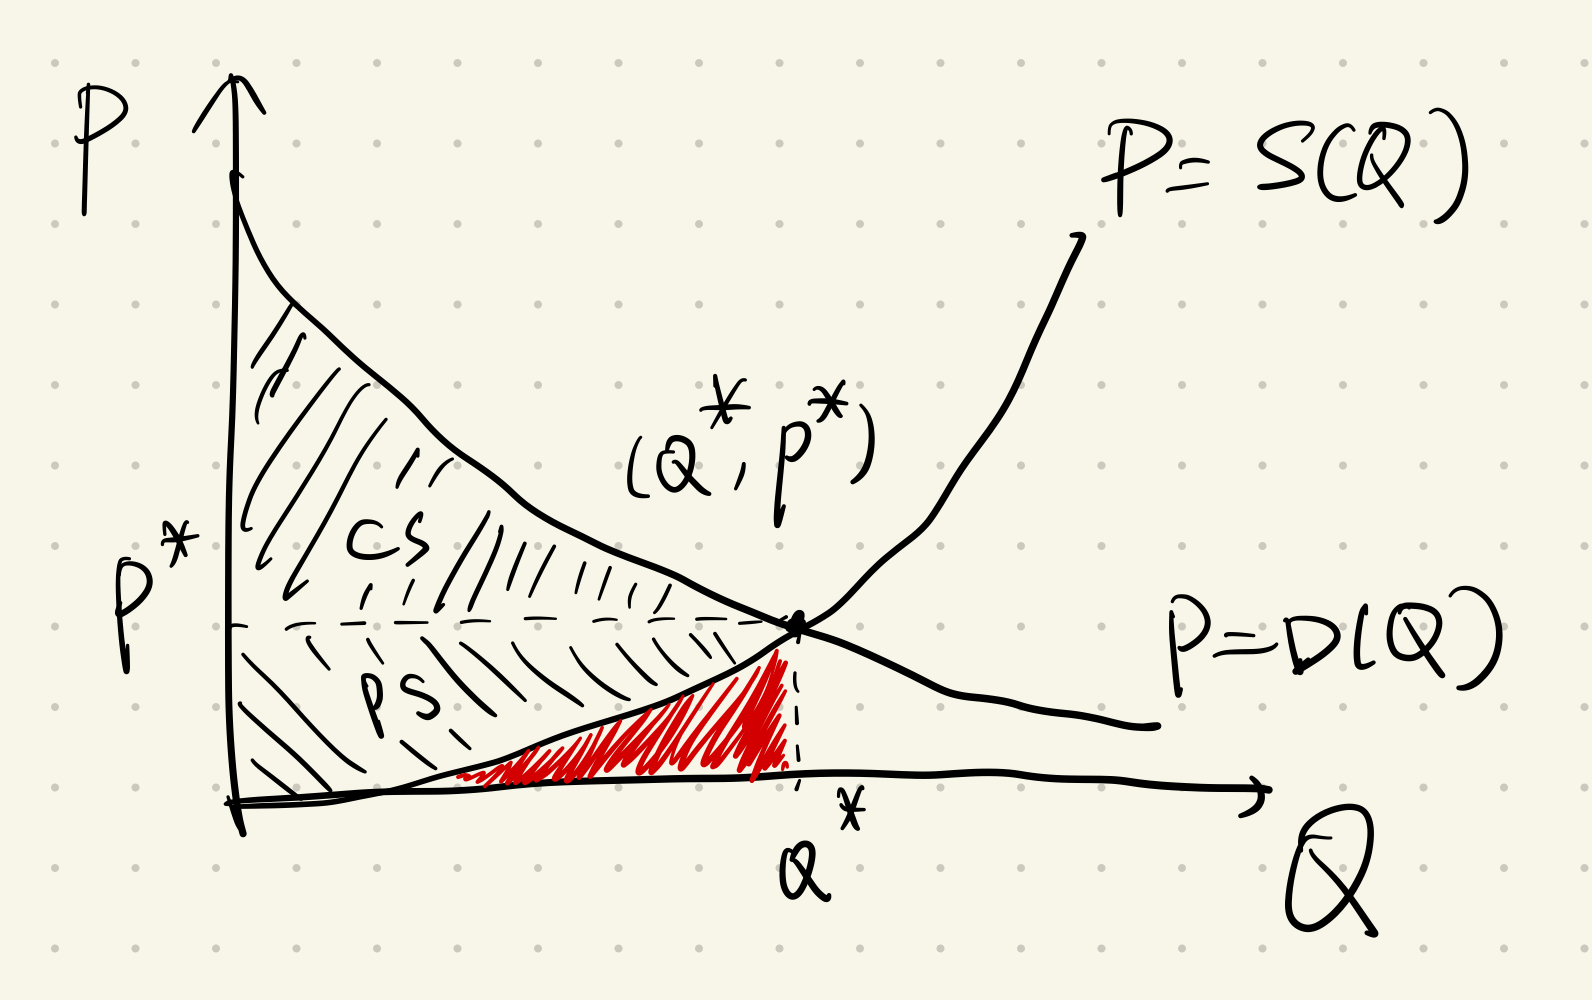
\includegraphics[width = 0.7\textwidth]{figures/chap 07/supply_demand.png}
\end{figure}

\medskip
A side note is that, in the example above, $D(Q)$ and $S(Q)$ are always positive, so it makes sense to talk about area \textit{under} the curve.  However, for functions taking negative values like the what the following graph depicts, the area bound by the curve and the $x$-axis is actually \textit{above} the curve.  In this case, for mathematical consistency, we use the notion of \textbf{signed area}, where areas above the curve and under the $x$-axis like this is given a negative sign.  With the concept of area-under-curve and signed area established, we can now define definite integrals as follows:

\begin{figure}[ht]
    \centering
    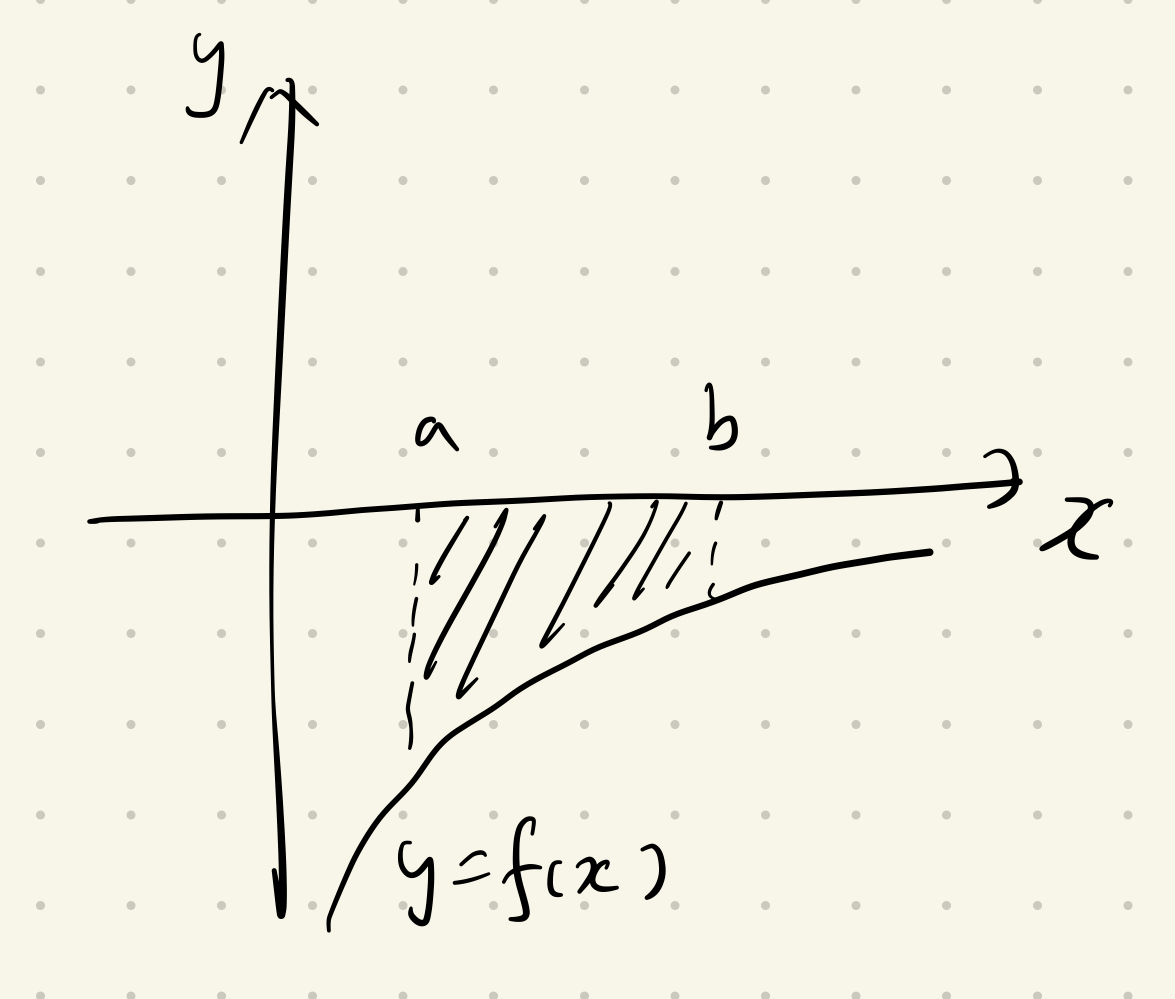
\includegraphics[width = 0.5\textwidth]{figures/chap 07/signed_area.png}
\end{figure}

\begin{defi}[Definite integrals]{def: definite_integral}
    Let $f(x)$ be a continuous function on a closed interval $[a,b]$.  The signed area bounded by the curve of $f(x)$, the $x$-axis, $x=a$ and $x=b$ is called the \textbf{definite integral} of $f(x)$ from $a$ to $b$, denoted by
    \[\int_a^b f(x)~dx\]
    where $a$ and $b$ are termed the lower and upper limit of integration for the definite integral.
\end{defi}

From this definition, if we go back to our previous example, we can notate the cosumer and producer surplus by:
\begin{align*}
    \text{Consumer surplus} &= \Big[\int_0^{Q^*} D(Q) dQ\Big] - P^*Q^*\\
    \text{Producer surplus} &= P^*Q^* - \Big[\int_0^{Q^*} S(Q) dQ\Big]
\end{align*}

Note that since definite integrals represent areas under curve, we have the following identities for definite integrals:
\begin{itemize}
    \item $\int_a^b kf(x)~dx = k\int_a^b f(x)~dx$
    \item $\int_a^b [f(x) \pm g(x)]~dx = \int_a^b f(x)~dx \pm \int_a^b g(x)~dx$
    \item $\int_a^b f(x)~dx = \int_a^c f(x)~dx + \int_c^b f(x)~dx$
    \item $\int_a^a f(x)~dx = 0$
    \item $\int_a^b f(x)~dx = -\int_b^a f(x)~dx$
\end{itemize}
where in the third identity, the area under $f(x)$ between $x = a$ and $x = b$ is intuitively decomposed into the sum of area under curve between $x = a$ and $x = c$, and area under curve between $x = c$ and $x = b$.  Setting $c = a$ in the third identity would lead to 
\[\int_a^b f(x)~dx = \int_a^a f(x)~dx + \int_a^b f(x)~dx\]
\[0 = \int_a^a f(x)~dx\]
which is exactly the fourth identity.  Setting $b = a$ in the third identity would instead lead to
\[\int_a^a f(x)~dx = \int_a^c f(x)~dx + \int_c^a f(x)~dx\]
\[\int_c^a f(x)~dx = -\int_a^c f(x)~dx \]
which implies the fifth identity: switching the upper and lower limit of a definite integral adds a negative sign to it. 

Some definite integrals can be evaluated using our knowledge in geometry.  Let's look at the following examples:

\begin{eg}[]{eg: definite_integrals}
    Using the definition of definite integrals, evaluate the following expressions:
    \begin{tasks}(3)
        \task $\int_0^2 (3x+1)~dx$
        \task $\int_2^4 (2x-5)~dx$
        \task $\int_3^1 \sqrt{4-(x-1)^2}~dx$
    \end{tasks}
\end{eg}

\begin{egsol}[]{egsol: definite_integrals}
    \begin{enumerate}[a)]
        \item If we graph $f(x) = 3x+1$ on the Cartesian plane, we see that the area under the curve from $x=0$ to $x=2$ forms a trapezoid shown in the graph below.  The two bases of the trapezoid are $f(0) = 1$ and $f(2) = 7$, and its height is $2$, so the area would be $\frac{(7+1)\cdot 2}{2} = 8$.  Therefore, the definite integral evaluates to $8$.

        \medskip
        \begin{center}
            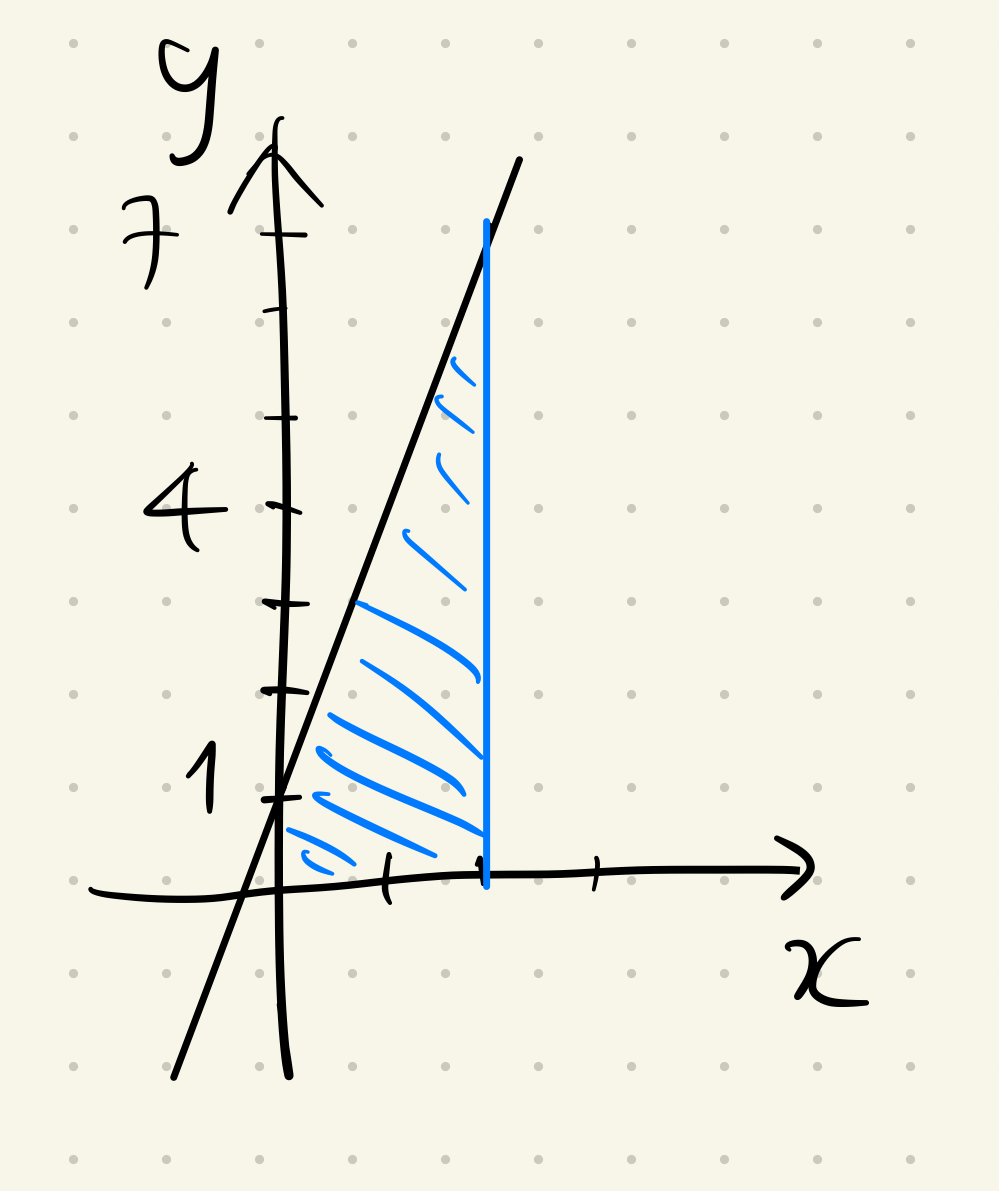
\includegraphics[width = 0.3\textwidth]{figures/chap 07/def_int_a.png}
        \end{center}
        \item If we graph $f(x) = 2x-5$ on the Cartesian plane, we see that between $x = 2$ and $x = 4$, part of the function is below the $x$-axis, and part of it is above the axis.  Since definite integrals are defined as signed area under the curves, we'll have to subtract the triangle below the axis from the triangle above the axis.  Using the identity of similar triangles, we know that since the height of the two triangles are $f(4) = 3$ and $|f(2)|=1$, their bases should be $2\cdot\frac{3}{1+3} = \frac{3}{2}$ and $2\cdot\frac{1}{1+3} = \frac{1}{2}$.  Therefore, the definite integral should evaluate to $\frac{3\cdot3/2}{2}-\frac{1\cdot1/2}{2} = 2$.
        
        \medskip
        \begin{center}
            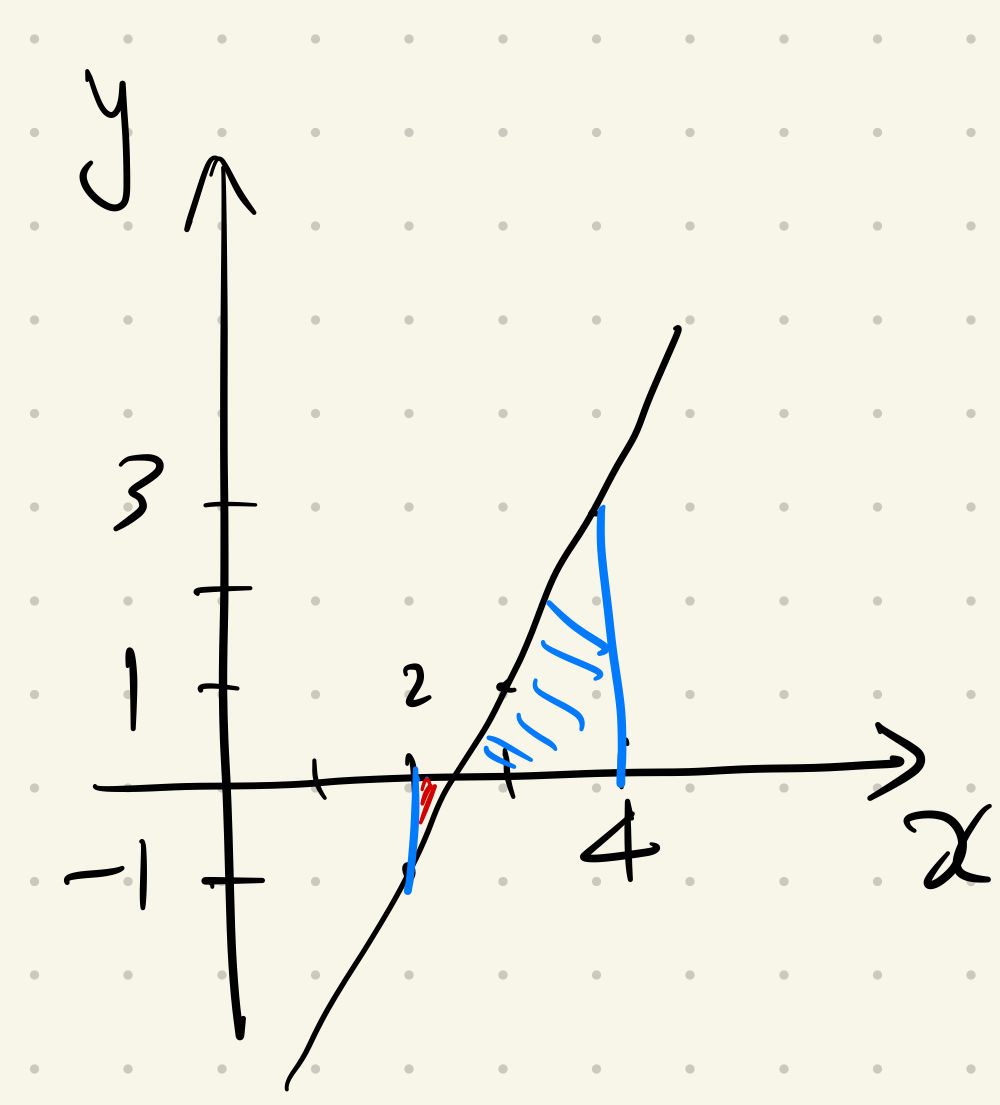
\includegraphics[width = 0.3\textwidth]{figures/chap 07/def_int_b.png}
        \end{center}
        \item Before we start graphing the function, note that upper limit of integration is smaller than its lower limit of integration, which is against our original definition.  However, using the identity we derived above, we can write
        \[\int_3^1 \sqrt{4-(x-1)^2}~dx = - \int_1^3 \sqrt{4-(x-1)^2}~dx\]
        Now the upper limit is larger than the lower limit, we can graph $f(x) = \sqrt{4 - (x-1)^2}$ on the Cartesian plane.  Rearranging $y = \sqrt{4 - (x-1)^2}$ yields $(x-1)^2 + y^2 = 2^2$, which implies that the curve of $f(x)$ is a half circle centered at $(1,0)$ with radius $2$.  Therefore, the area under the curve between $x=1$ and $x=3$ is a quarter of the circle, which has area $\pi\cdot(2)^2/4 = \pi$.  Therefore, our original definite integral evaluates to $-\pi$.
        
        \medskip
        \begin{center}
            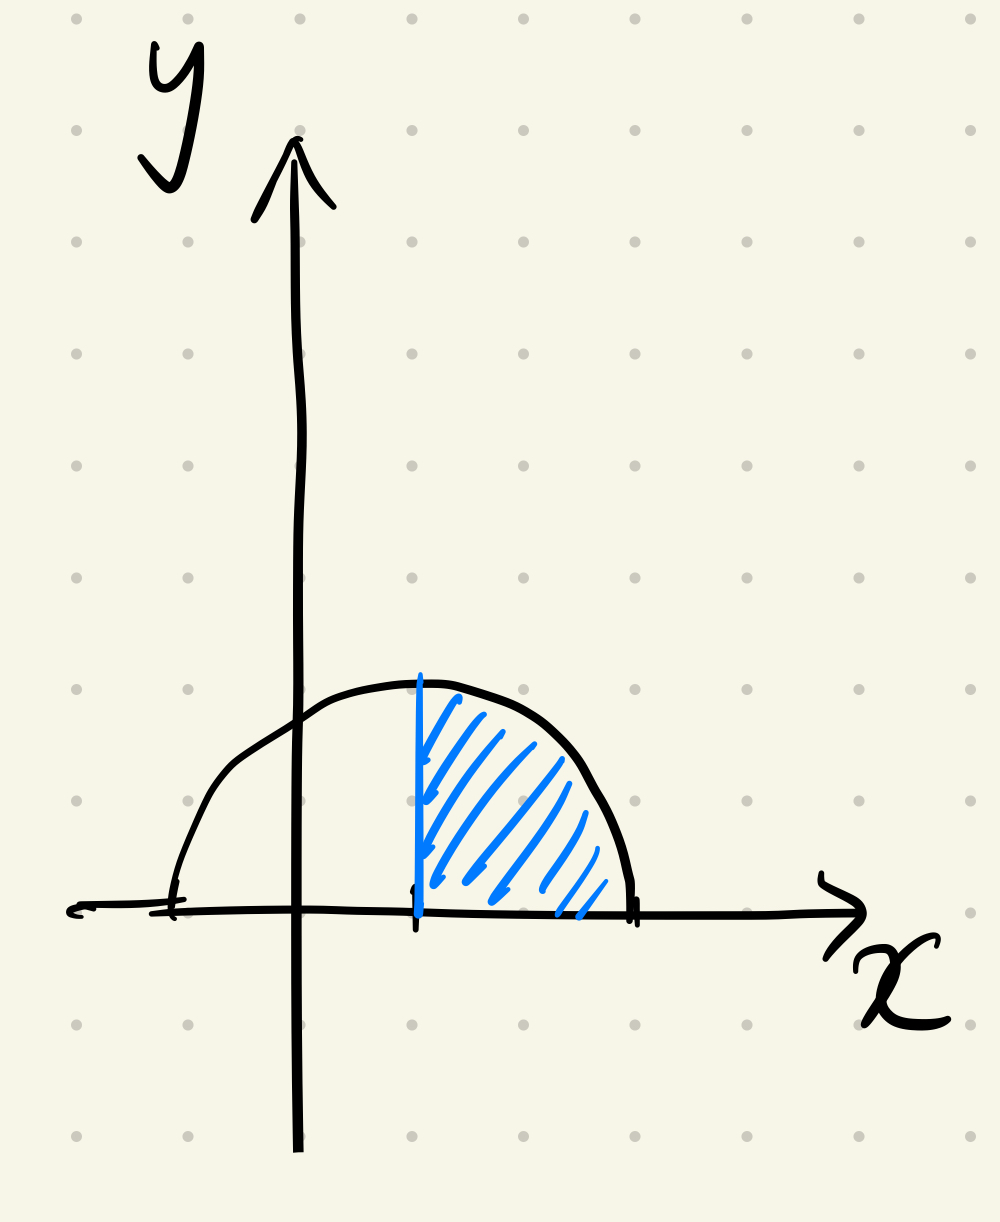
\includegraphics[width = 0.3\textwidth]{figures/chap 07/def_int_c.png}
        \end{center}
    \end{enumerate}
\end{egsol}

In the example above, the functions to be integrated represent straight lines and circles, so the area under the curves all formed shapes we are familiar with.  However, when the functions do not represent lines and circles, evaluating the integral will be much more difficult.  For example, suppose we would like to like to evaluate $\int_0^2 x^2~dx$, whose integrand is a upward-facing parabola as shown in the graph below.  One way to approach the area under curve is to first split the integration interval into smaller subintervals.  For example, in the graph, we split $[0, 2]$ into $8$ subintervals of length $\Delta x_{(8)} = 2/8$.  Then, the area under the curve can be approximated by the sum of the area of the blue bars, each with width $\Delta x_{(8)}$ and height $f(0 + j \Delta x_{(8)})$, where $j$ is the index of the subintervals ranging from $1$ to $8$.  We can write the approximation as
\begin{align*}
    \hat{A}_8 &= (f(0 + \Delta x_{(8)}) + f(0 + 2\Delta x_{(8)}) + f(0 + 3\Delta x) + ... + f(0 + 8 \Delta x_{(8)}))\Delta x_{(8)}\\
    &= \Big[\sum_{j=1}^8 f(0+j \Delta x_{(8)})\Big]\Delta x_{(8)}\\
    &= \Big[\sum_{j=1}^8 j^2 \Delta x_{(8)}^2\Big]\Delta x_{(8)}\\
    &= \Big[\sum_{j=1}^8 j^2\Big] \Delta x_{(8)}^3 =  \Big[\sum_{j=1}^8 j^2\Big] \Big(\frac{2}{8}\Big)^3 = 204 \cdot \Big(\frac{1}{4}\Big)^3 = \frac{51}{16}
\end{align*}

\begin{figure}[ht]
    \centering
    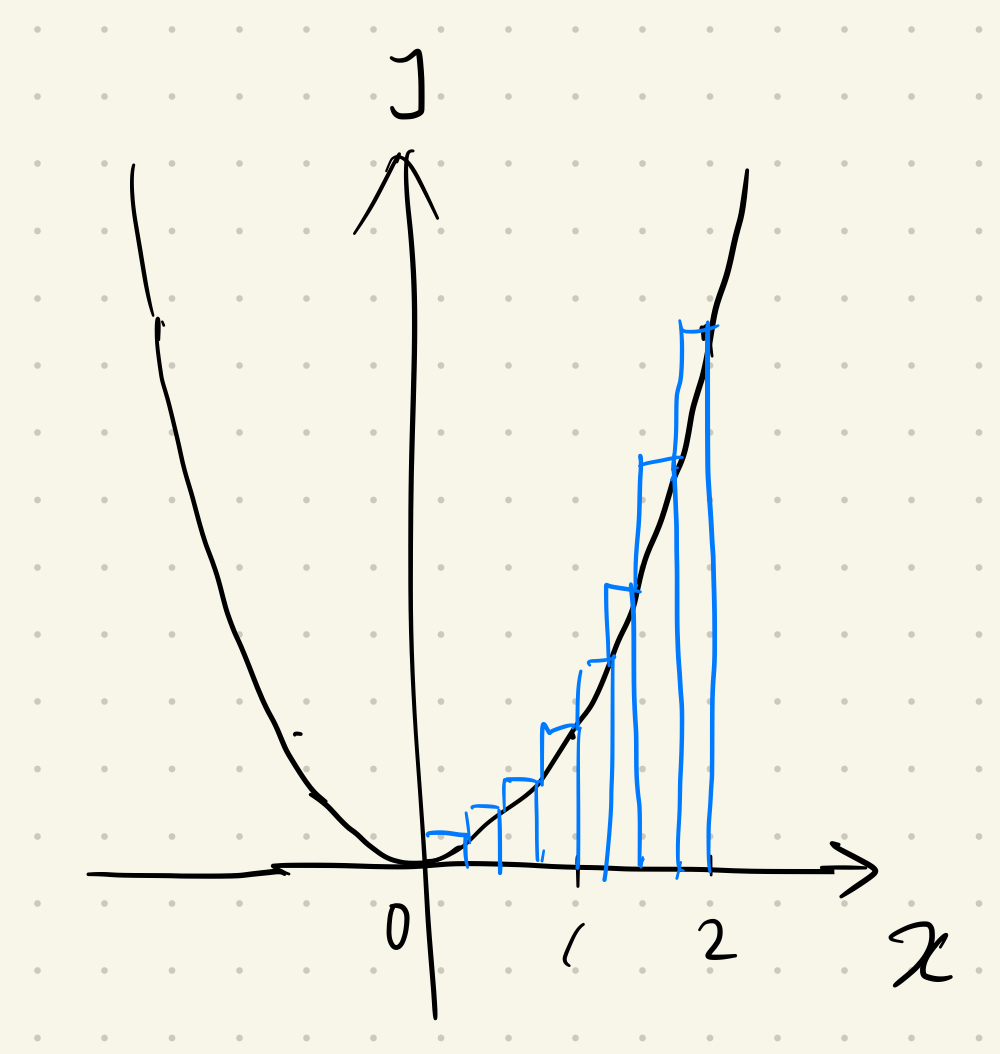
\includegraphics[width = 0.45\textwidth]{figures/chap 07/def_int_series.png}
\end{figure}

This approximation is called a (right) Riemann sum.  If we notate the number of subintervals as $n$ so that the length of the subintervals is $\Delta x_{(n)} = 2/n$, we yield a generalized Riemann sum:
\[\hat{A}_n = \Big[\sum_{j=1}^n j^2\Big] \Delta x_{(n)}^3 = \frac{n(n+1)(2n+1)}{6} \Big(\frac{2}{n}\Big)^3 = \frac{4n(n+1)(2n+1)}{3n^3}\]
where the second equality uses the formula for sum of squares of the first $n$ positive numbers.  Note as $n$ increases, the bars will be finer and finer, and the sum of the bars will eventually approach to the area under the curve.  Therefore, we can write our definite integral as a limit with $n$ approaching infinity:
\[\int_0^2 x^2~dx = \lim_{n \rightarrow \infty} \hat{A}_n = \lim_{n \rightarrow \infty} \frac{4n(n+1)(2n+1)}{3n^3} = \frac{8}{3}\]
where the last equality comes from the ratio of leading coefficients.

Here, we used the limit of Riemann sums to evaluate the definite integral, which is not an easy feat.  However, our success is not without luck: because our integrand is $x^2$, the sum of squares of the first $n$ positive numbers appeared in the Riemann sum, which we happened to know a clean formula for the sum.  If our integrand was something gnarlier, then it may well be the case that we do not have a closed form expression for the Riemann sum, and thus cannot take its limit.  In light of this, we will need a more general procedure to evaluate definite integrals. 

To develop the procedure, first we define an \textbf{area function} as a definite integral that leaves its upper limit as input.  For example, in the graph below, we define the area function $F(x) = \int_0^x f(t)~dt$, where the lower limit of integration is fixed at $0$ but the upper limit of integration is the variable $x$.  The signed area $F(x)$ represents is then by definition the area shaded blue.  

\begin{figure}[ht]
    \centering
    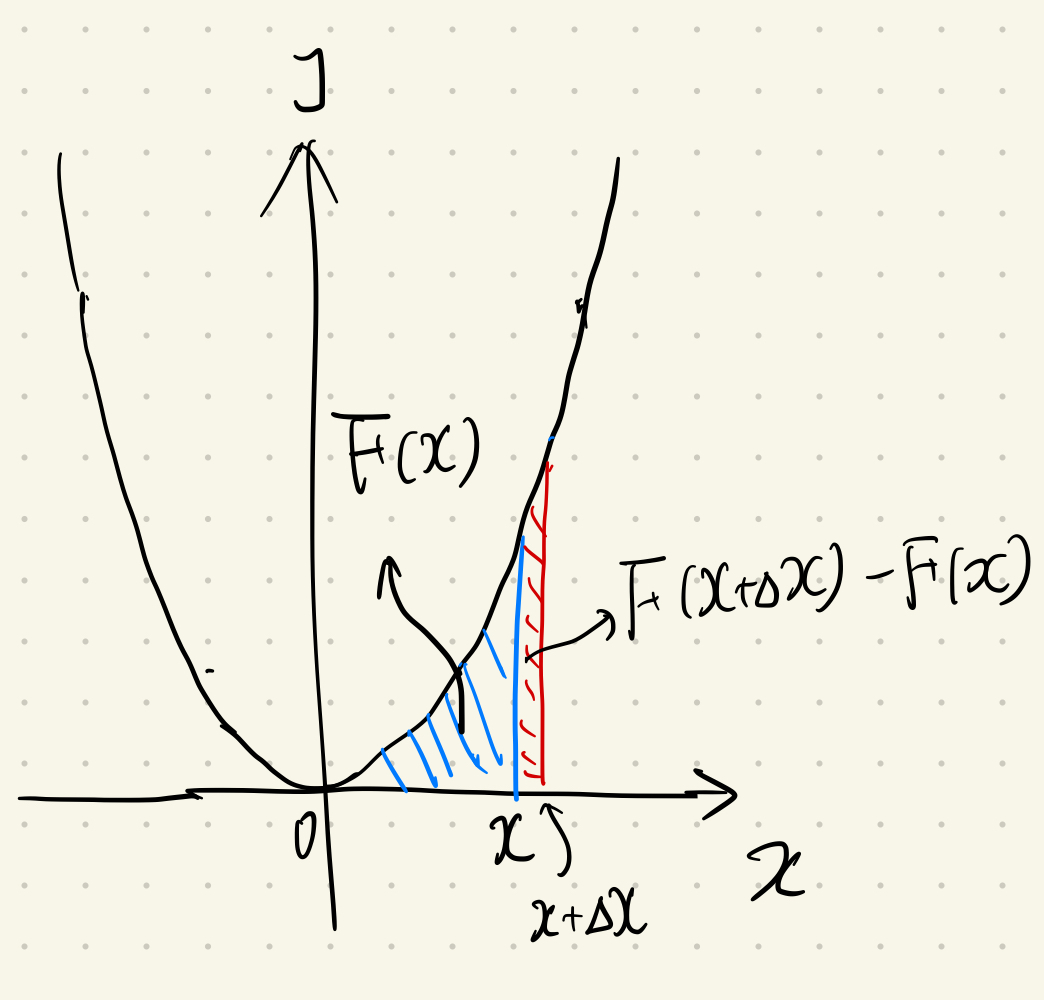
\includegraphics[width = 0.45\textwidth]{figures/chap 07/FTC.png}
\end{figure}

Now for a small $\Delta x$, the difference between $F(x+\Delta x)$ and F(x) would be the small strip of area under curve from $x$ to $x + \Delta x$, which is the area shaded red in the graph.  As $\Delta x$ gets smaller and smaller, the area of the strip would be closer and closer to $f(x) \Delta x$.  In other words, as $\Delta x$ gets smaller and smaller, the ratio between $F(x + \Delta x) - F(x)$ and $\Delta x$ would approach $f(x)$.  Therefore, we have

\[\frac{dF}{dx} = \lim_{\Delta x \rightarrow 0} \frac{F(x + \Delta x) - F(x)}{\Delta x} = f(x)\]

which implies that $F(x)$, which we originally defined as an area function, is actually an antiderivative of $f(x)$!  This remarkable result serves as a bridge between integral calculus (definite integrals) to differential calculus (antiderivatives), which we formally state in the theorem below:

\begin{theo}[Fundamental Theorem of Calculus, First Part]{thm: FTC1}
    Let $f(x)$ be a continuous function on $[a, b]$. Suppose $F(x)$ is an area function defined as 
    \[F(x) = \int_a^x f(t) dt, \quad x \in (a,b)\]
    then $F'(x) = f(x)$ for all $x \in (a,b)$.
\end{theo}

However, note that the first part of the Fundamental Theorem of Calculus only tells us that the area function $F(x)$ is \textit{an} antiderivative of $f(x)$, but does not tell us \textit{which} antiderivative it is.  That is, it does not explicitly tell us what the integration constant should be when we have obtained our antiderivative.  Fortunately, the second part of the Fundamental Theorem of Calculus tells us that as long as we are only interested in evaluating the definite integral, the choice of integration constant does not matter (it also relaxes the requirement for $f(x)$ to be continuous, but here we will not dig deeper into this issue):

\medskip
\begin{theo}[Fundamental Theorem of Calculus, Second Part]{thm: FTC2}
    Let $f(x)$ be a function on $[a, b]$.  Let $F(x)$ be \textit{any} antiderivative for $f(x)$, then
    \[\int_a^b f(x) dx = F(b) - F(a)\]
\end{theo}

Therefore, to find the definite integral for $f(x)$ from $a$ to $b$, we just need to find \textit{one} antiderivative for $f(x)$, and subtract its value at $x = b$ by its value at $x = a$.  Here since antiderivatives are closely linked to the evaluation of definite integrals, they are alternatively termed as \textbf{indefinite integrals}.

Let us try out our new evaluation method for definite integrals with a few examples:

\begin{eg}[]{eg: def_int_FTC}
    Evaluate the following definite integrals
    \begin{tasks}(3)
        \task $\int_0^2 x^2~dx$
        \task $\int_{\pi/2}^{0} \sin x~dx$
        \task $\int_1^{\sqrt{3}} \frac{1}{x^2+1}~dx$
        \task $\int_0^1 \frac{x}{x^2+1}~dx$
        \task $\int_{1/2}^{\sqrt{3}/2} \frac{1}{(\sqrt{1-x^2})^3}~dx$
        \task $\int_{0}^{\pi/4} x \cos x~dx$
    \end{tasks}
\end{eg}

\begin{egsol}[]{egsol: def_int_FTC}
    \begin{enumerate}[a)]
        \item We have evaluated this definite integral the hard way using Riemann sums.  Now let us try using antiderivatives and the Fundamental Theorem of Calculus.  Since one antiderivative of $x^2$ is $\frac{1}{3}x^3$, we can write:
        \[\int_0^2 x^2~dx = \frac{1}{3}x^3\Big]^2_0 = \frac{1}{3}(2)^3 - \frac{1}{3}(0)^3 = \frac{8}{3}\]
        where the notation $g(x)\big]^b_a$ stands for $g(b)-g(a)$.  Antiderivatives have indeed saved us much time here.
        \item Since one antiderivative of $\sin x$ is $-\cos x$, we have
        \[\int_{\pi/2}^0 \sin x~dx = (-\cos x)\Big]_{\pi/2}^0 = -\cos(0) + \cos(\pi/2) = -1 + 0 = -1\]
        Note here we do not even care if the upper limit of integration is larger than the lower limit.  We can just evaluate our antiderivatives with the correct order of subtraction, and the Fundamental Theorem of Calculus will take care of the rest.
        \item Remember that one antiderivative of $\frac{1}{x^2+1}$ is $\arctan x$, so we have
        \[\int_1^{\sqrt{3}} \frac{1}{x^2+1}~dx = \arctan x\Big]_1^{\sqrt{3}} = \arctan(\sqrt{3}) - \arctan(1) = \frac{\pi}{3} - \frac{\pi}{4} = \frac{\pi}{12}\]
        \item The antiderivative for this integrand is not immediately obvious, but if we try U-substituion with $u = x^2+1$, we have $du = 2xdx$, which works since the remainder of the integrand is $x$.  Therefore, we have
        \[\int_0^1 \frac{x}{x^2+1} dx = \frac{1}{2}\int_0^1 \frac{1}{x^2+1}(2xdx)\]
        Now note that when we preform variable substitutions in definite integrals, we will also have to substitute the limits of integration.  That is, originally we are integrating from $x = 0$ to $x = 1$, but now we are changing our variable for integration to $u$, the limits of integration should then be from $u = 0^2+1 = 1$ to $u = 1^2 + 1 = 2$.  We then yield
        \[\frac{1}{2}\int_0^1 \frac{1}{x^2+1}(2xdx) = \frac{1}{2} \int_1^2 \frac{1}{u} du = \frac{1}{2}(\ln |u|)\Big]_1^2 = \frac{1}{2}(\ln |2| - \ln |1|) = \frac{\ln 2}{2}\]
        \item The $\sqrt{1-x^2}$ in the denominator screams for a trigonometric substitution where $x = \sin \theta$ and $dx = \cos \theta d\theta$, but note that since we are performing variable substitution, we need to also transform the limits of integration.  This is where the range setting for $\theta$ becomes important.  Since we by convention set $-\pi/2 \le \theta \le \pi/2$, we have when $x = 1/2$ and $\sqrt{3}/2$, $\theta = \pi/6$ and $\pi/3$. Therefore we yield
        \begin{align*}
            \int_{1/2}^{\sqrt{3}/2} \frac{1}{(\sqrt{1-x^2})^3}~dx &= \int_{\pi/6}^{\pi/3} \frac{1}{\cos^3 \theta}\cos \theta d\theta\\
            &= \int_{\pi/6}^{\pi/3} \sec^2 \theta d\theta\\
            &= \tan \theta \Big]_{\pi/6}^{\pi/3}\\
            &= \tan\Big(\frac{\pi}{3}\Big) - \tan\Big(\frac{\pi}{3}\Big) = \sqrt{3} - \frac{1}{\sqrt{3}} = \frac{2}{3}\sqrt{3}
        \end{align*}
        \item Here the antiderivative can be found using integration by parts setting $u = x$ and $dv/dx = \cos x$, so that $du/dx = 1$ and $v = \sin x$.  Therefore we have
        \begin{align*}
            \int_{0}^{\pi/4} x \cos x~dx &= x \sin x \Big]_{0}^{\pi/4} - \int_{0}^{\pi/4} \sin x~dx\\
            &= x \sin x \Big]_{0}^{\pi/4} + \int_{0}^{\pi/4} (-\sin x)~dx\\
            &= x \sin x \Big]_{0}^{\pi/4} + \cos x \Big]_{0}^{\pi/4}\\
            &= \Big(\frac{\pi}{4} \sin \frac{\pi}{4} - 0 \sin 0\Big) + \Big(\cos \frac{\pi}{4} - \cos 0 \Big)\\
            &= \frac{\pi}{4} \cdot \frac{\sqrt{2}}{2} + \frac{\sqrt{2}}{2} - 1 = \frac{\sqrt{2}}{8}\pi + \frac{\sqrt{2}}{2}- 1
        \end{align*}
        Note that since this is a definite integral, the "$uv$" term is also subject to calculation of value difference at limits of integration, so don't forget to put a right bracket beside it!
    \end{enumerate}
\end{egsol}

\section{Area and arc length}

In the previous section we defined definite integrals as the area under the curve of a function, and showed that definite integrals can be promptly evaluated using antiderivatives.  However, definite integrals can do much more than calculating the area under the curve.  

To extend the use of definite integrals, first recall that back when we did not know how to use antiderivatives to evaluate definite integrals, we turned to the limit of Riemann sums, which can be written and graphed as follows 
\[\int_a^b f(x) dx = \lim_{\Delta x \rightarrow 0} \sum_{i=1}^n f(x_i) \Delta x\]
\begin{figure}[ht]
    \centering
    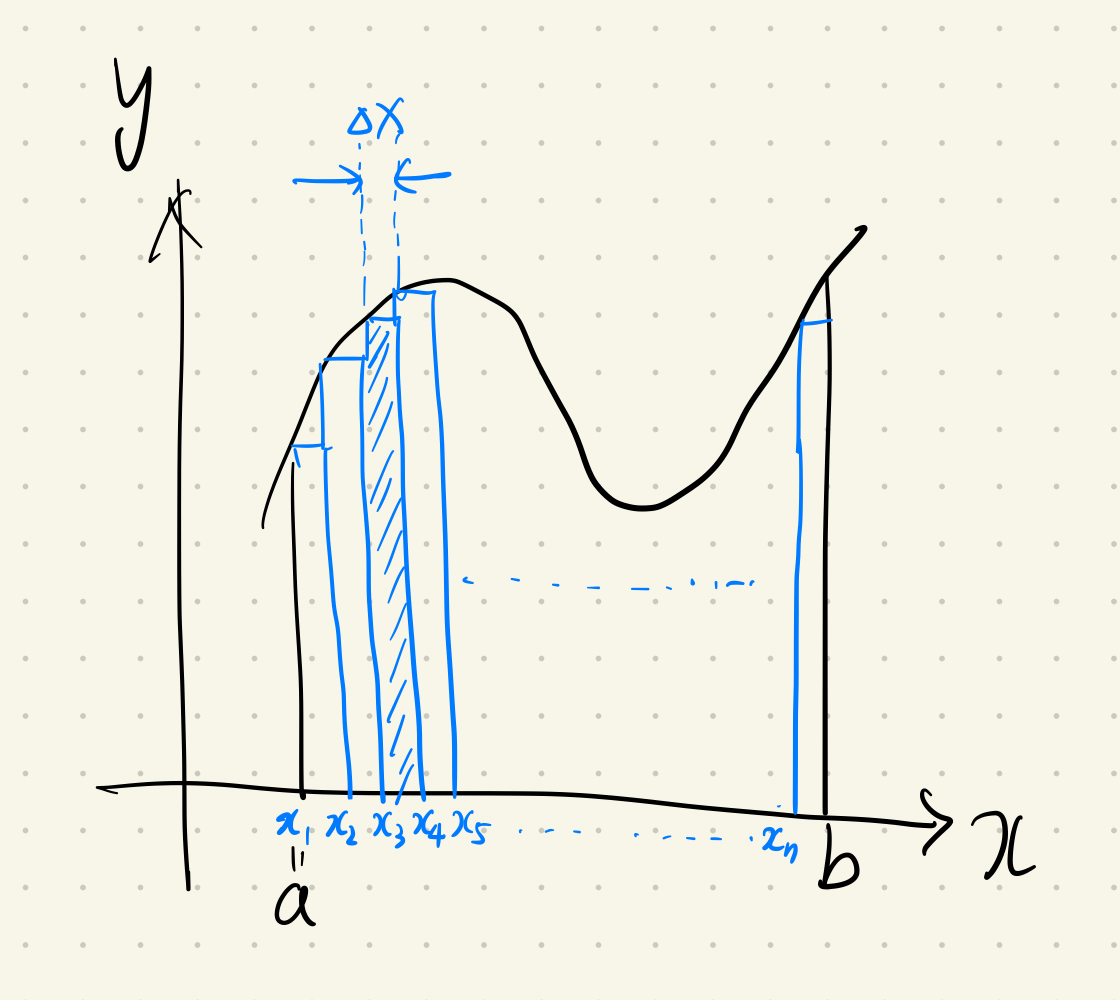
\includegraphics[width = 0.5\textwidth]{figures/chap 07/Riemann.png}
\end{figure}

\bigskip
In the right hand side, the term $f(x_i) \Delta x$ is the area of the strip of rectangle at $x = x_i$ with width $\Delta x$.  For example, $f(x_3)\Delta x$ represents the area of the blue strip shown in the graph.  Then, the summation sign adds all the strips up, with the $x$-coordinates of the strip ranging from $a$ to $b$.  Roughly speaking, as $\Delta x$ goes to zero, $f(x_i)\Delta x$ can be replaced with $f(x)dx$, and the summation sign can be replaced with $\int_a^b$, which re-frames the limit of summation into limit of integration.  The limit of integration specifies the limit of the variable indicated by the differential, which in this case is $x$.

With this correspondence in mind, we do not have to resort to writing out the limit of Riemann sums everytime we want to find a definite integral.  Instead, as shown in the left panel below, we can directly say that the area under $y = f(x)$ between $x = a$ and $x = b$ is just adding up the area of small shaded strips while $x$ goes from $a$ to $b$.  Since the area of the small strips is $f(x)dx$, we write the area as $\int_a^b f(x)dx$. 

\begin{figure}[ht]
    \centering
    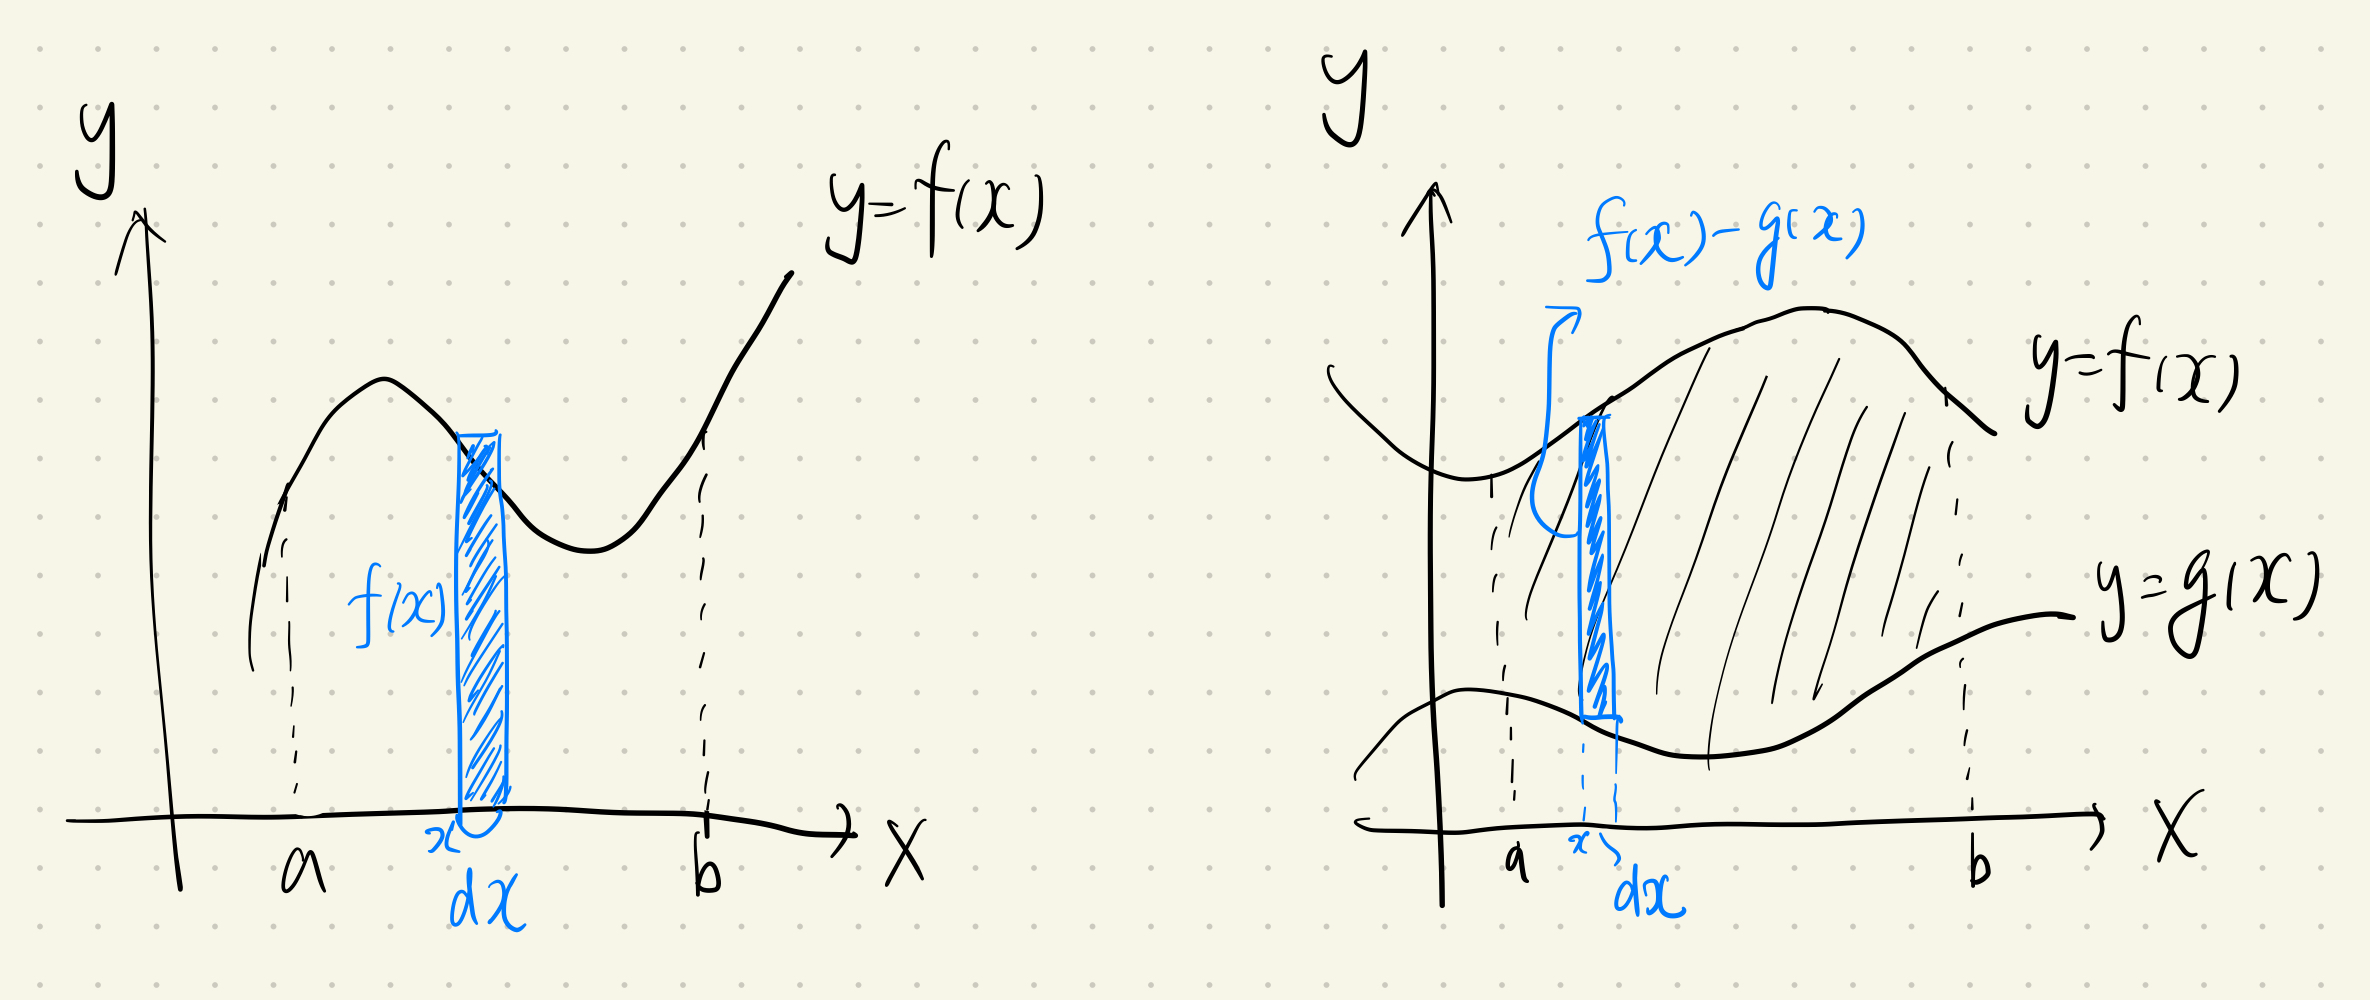
\includegraphics[width = 0.8\textwidth]{figures/chap 07/Differential_Riemann.png}
\end{figure}

This method of constructing definite integrals can be extended to the evaluation of area between the curves of two functions.  As shown in the right panel of the graph above, suppose $f(x) \ge g(x)$ within $x \in [a,b]$, and we would like to find the area enclosed by $y = f(x)$, $y = g(x)$, $x=a$ and $x=b$.  We note that the area can broken up into the sum of small shaded strips as shown in the graph, with width $dx$ and height $|f(x)-g(x)| = f(x) - g(x)$, so that the area is $(f(x)-g(x))dx$.  Since the summation ranges from $x=a$ to $x=b$, our area of interest can be written as
\[A = \int_a^b (f(x)-g(x))dx\]
Notice that in this case we are assuming that $f(x) \ge g(x)$ within $[a, b]$.  If $f(x)$ is less than $g(x)$ in any interval within $[a,b]$, then the height of the strip within that interval would be $g(x)-f(x)$, so the integrand would become $g(x)-f(x)$.  In this case, we will have to evaluate the definite integral into different parts are evaluate them separately.  We will now demonstrate its application with several examples:

\begin{eg}[]{eg: area_between_functions}
    Find the following areas using definite integrals:
    \begin{enumerate}[a)]
        \item The area between $y = (x-1)^2 + 3$ and $y = -(x-2)^2$ from $x = 1$ to $x = 3$.
        \item The area enclosed by $y = \sqrt{x}$ and $y = x^2$
        \item The area enclosed by $y = \sin x$ and $y = \cos x$ between $x = \pi/4$ to $x = 5\pi/4$
        \item The area between $y = 2x$ and $y = x^3$ from $x = -1$ to $x = 1$
    \end{enumerate}
\end{eg}

\begin{egsol}[]{egsol: area_between_functions}
    \begin{enumerate}[a)]
        \item We first graph $y = (x-1)^2 +3$ and $y = -(x-2)^2$ as follows, which shows that $(x-1)^2 +3$ is always greater than $-(x-2)^2$ between $x = 1$ and $x = 3$.  Therefore, we can directly construct the definite integral as
        \begin{align*}
            &\int_1^3 [((x-1)^2 + 3) - (-(x-2)^2)]dx\\
            =& \int_1^3 [(x^2-2x+4)+(x^2-4x+4)]dx\\
            =& \int_1^3 (2x^2-6x+8) dx\\
            =& \Big(\frac{2}{3}x^3 - 3x^2 + 8x \Big)\Big]_1^3\\
            =& \Big(\frac{2}{3}\cdot 27 - 3 \cdot 9 + 8 \cdot 3 \Big) - \Big(\frac{2}{3} - 3 + 8 \Big)\\
            =& 15 - \frac{17}{3} = \frac{28}{3} 
        \end{align*}
        \begin{center}
            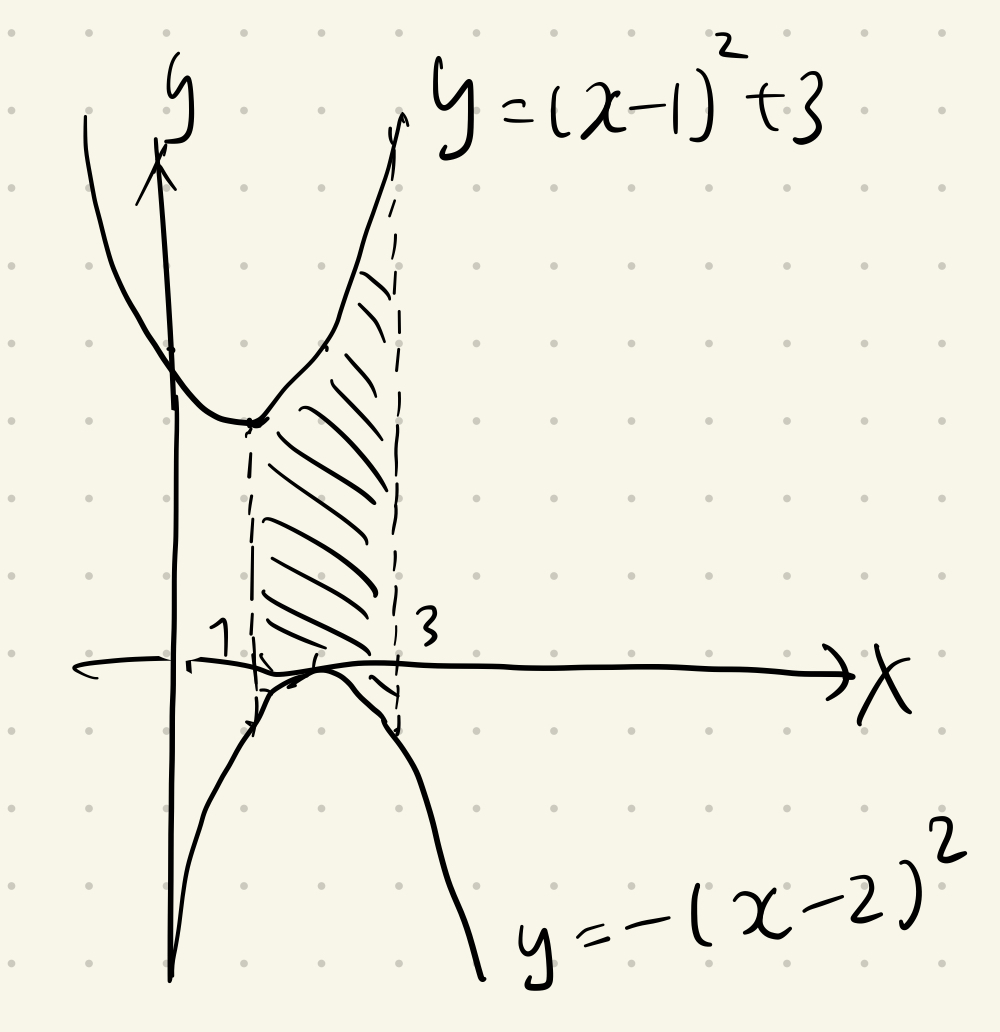
\includegraphics[width = 0.35\textwidth]{figures/chap 07/eg_7_3_a.png}
        \end{center}
        \item The problem did not give us the range of $x$ for the area enclosed by the two functions, so we first graph $y = x^2$ and $y = \sqrt{x}$.  As the following graph shows, they intersect at $(0,0)$ and $(1,1)$, and the enclosed area lies between these two points.  In addition, $\sqrt{x}$ is always no less than $x^2$ with in $x \in [0,1]$.  Therefore, we can directly construct the definite integral as
        \[\int_0^1(\sqrt{x} - x^2)~dx = \int_0^1(x^{1/2} - x^2)~dx = \Big(\frac{2}{3}x^{3/2} - \frac{1}{3}x^3\Big)\Big]_0^1 = \frac{2}{3} - \frac{1}{3} = \frac{1}{3}\]
        \begin{center}
            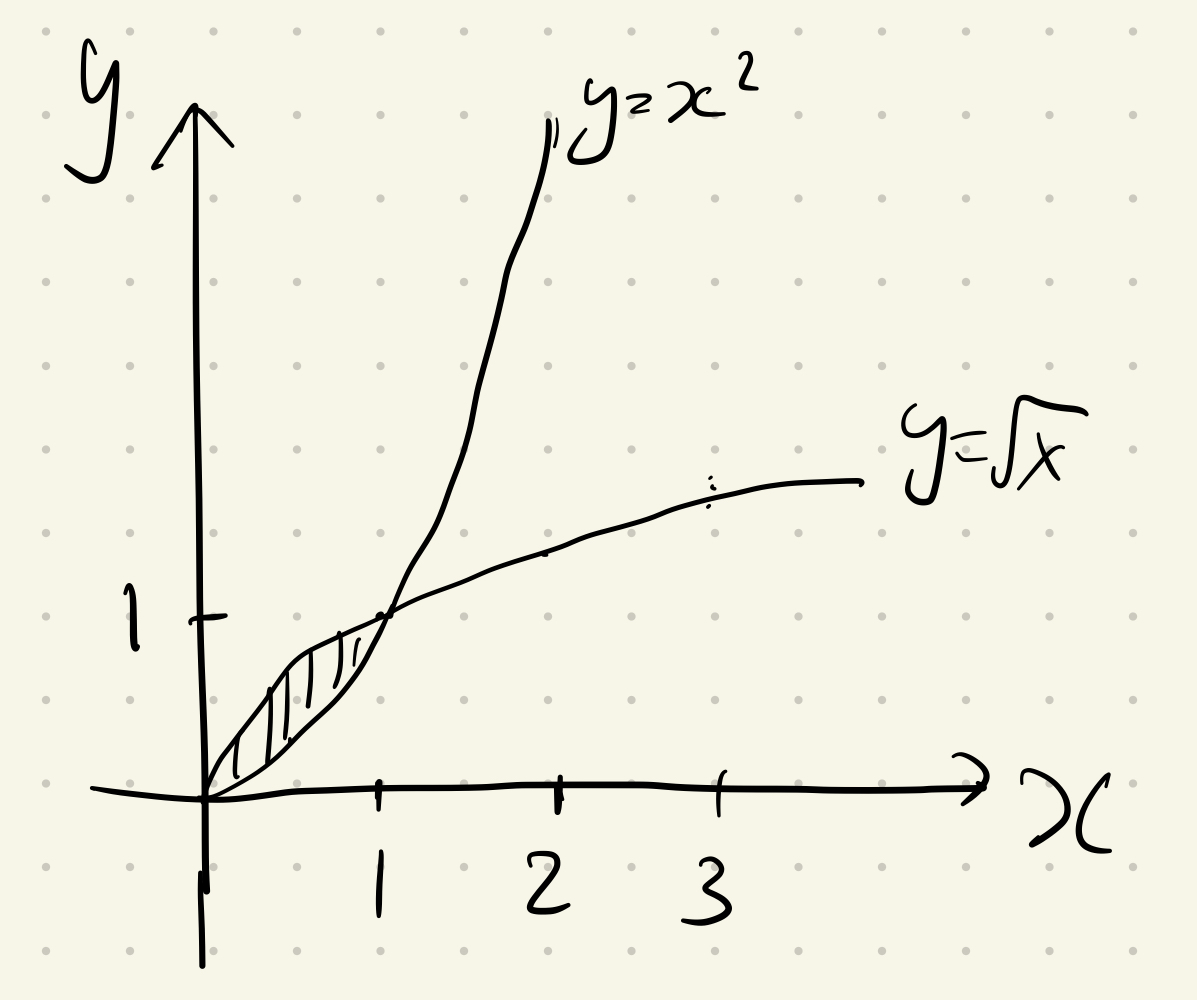
\includegraphics[width = 0.35\textwidth]{figures/chap 07/eg_7_3_b.png}
        \end{center}
        \item We first graph $y = \sin x$ and $y = \cos x$ within $x \in [\pi/4, 5\pi/4]$.  Notice that within $[\pi/4, 5\pi/4]$, we have $\sin x \ge \cos x$.  Therefore, we can directly construct the definite integral as
        \[\int_{\pi/4}^{5\pi/4} (\sin x - \cos x)~dx = (- \cos x - \sin x) \Big]_{\pi/4}^{5\pi/4} = \Big(\frac{1}{\sqrt{2}} + \frac{1}{\sqrt{2}}\Big)-\Big(-\frac{1}{\sqrt{2}} - \frac{1}{\sqrt{2}}\Big) = \frac{4}{\sqrt{2}} = 2\sqrt{2}\]
        \begin{center}
            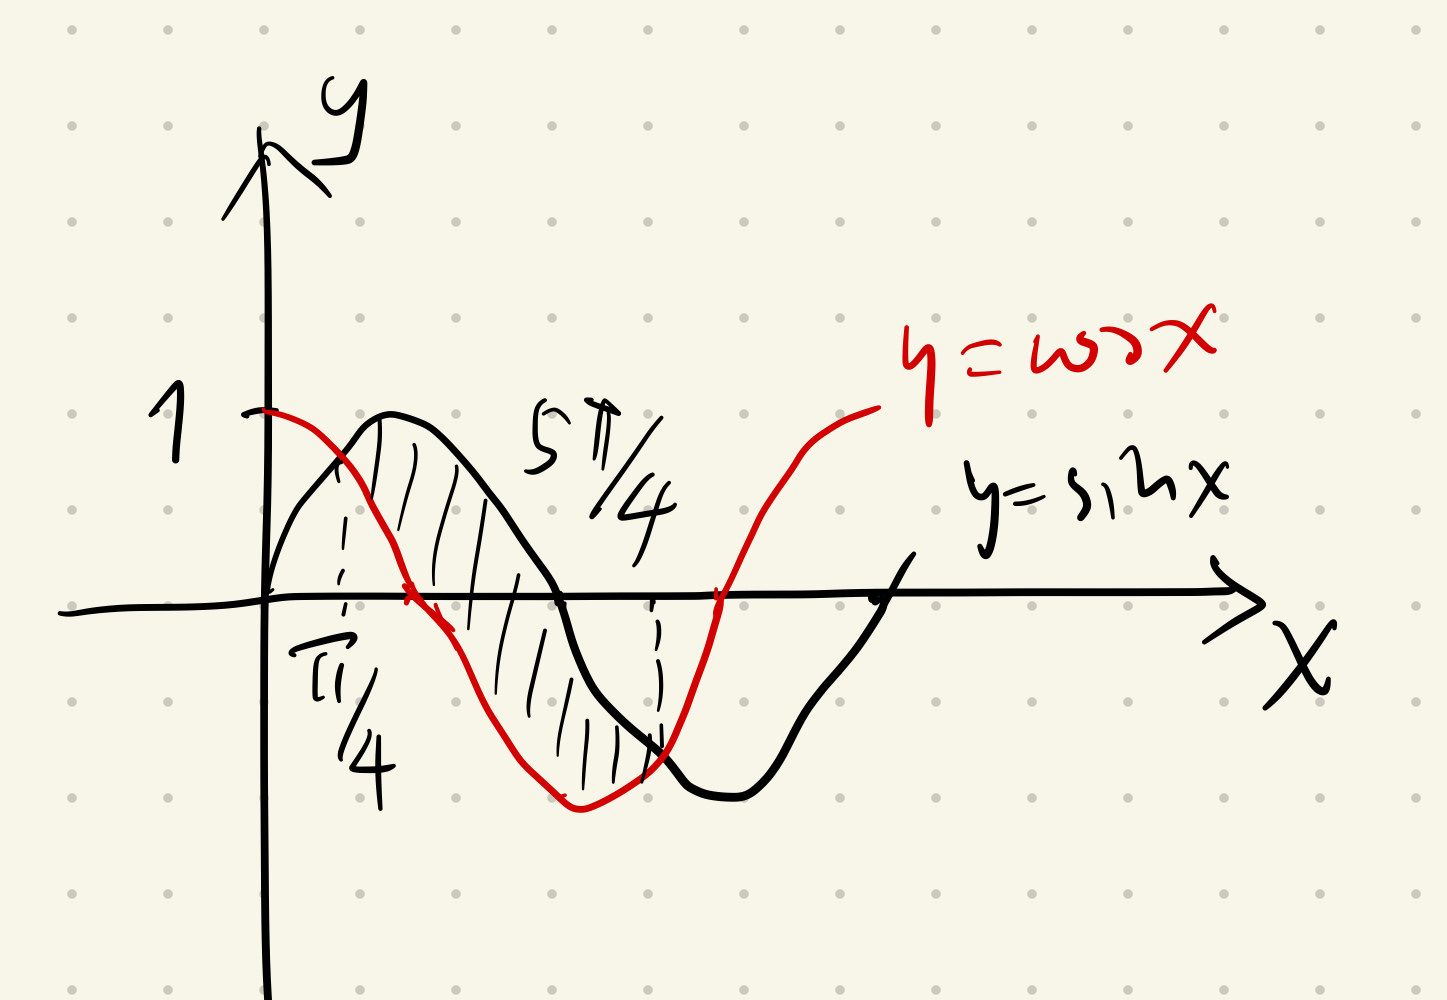
\includegraphics[width = 0.35\textwidth]{figures/chap 07/eg_7_3_c.png}
        \end{center}
        \item We first graph $y = 2x$ and $y = x^3$ within $x \in [-1, 1]$ as the follow graph, and notice that $2x > x^3$ when $x > 0$, but $x^3 > 2x$ when $x < 0$.  Therefore, we will have to construct the definite integral by splitting the range of integration into two parts, $[-1, 0]$ and $[0,1]$:
        \begin{align*}
            &\int_{-1}^0 (x^3-2x)~dx + \int_0^1 (2x-x^3)~dx\\
            =& \Big(\frac{1}{4}x^4 - x^2\Big)\Big]_{-1}^0 + \Big(x^2 - \frac{1}{4}x^4\Big)\Big]_0^1\\
            =& \Big[(0 - 0) - \Big(\frac{1}{4}-1\Big)\Big] + \Big[\Big(1 - \frac{1}{4}\Big)-(0-0)\Big] = \frac{3}{2}
        \end{align*}
        \begin{center}
            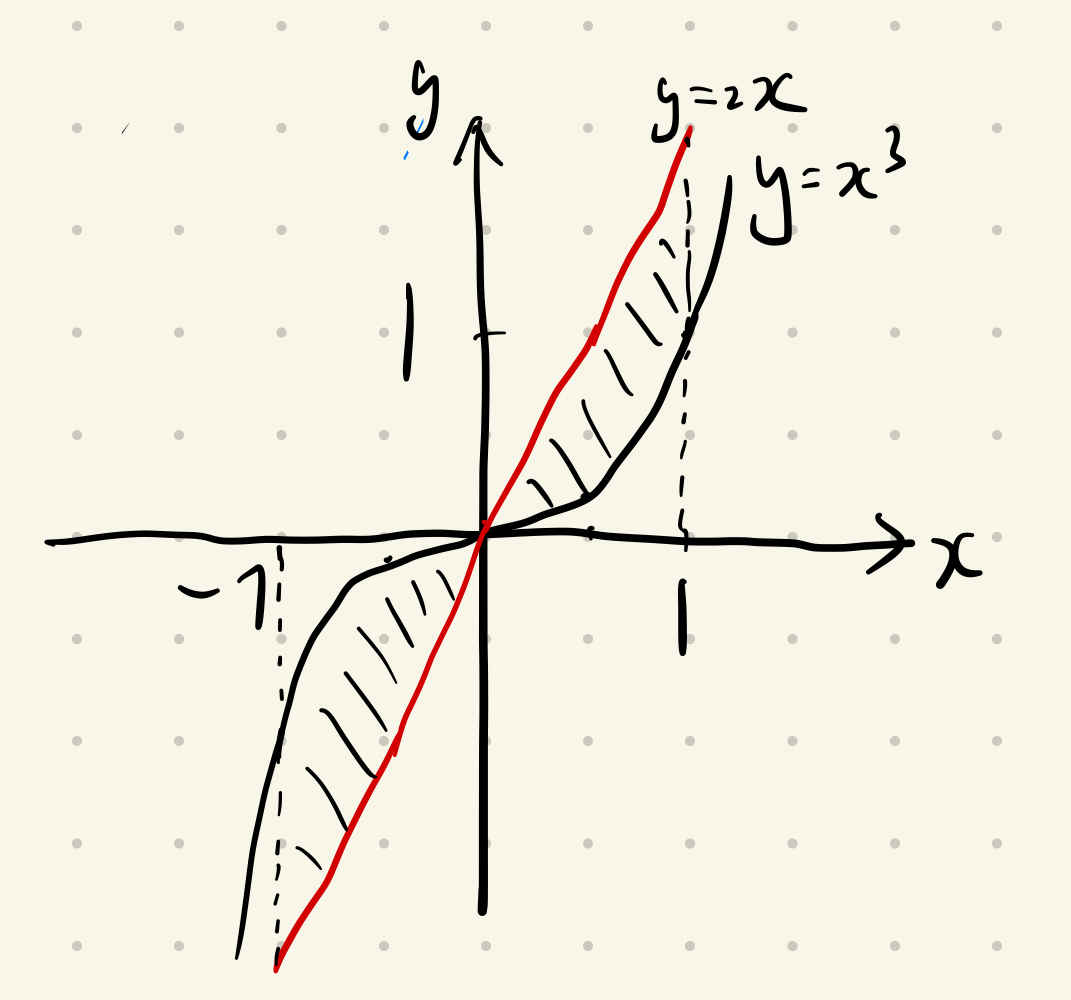
\includegraphics[width = 0.35\textwidth]{figures/chap 07/eg_7_3_d.png}
        \end{center}
        Notice that if we did not determine the order of $2x$ and $x^3$ first, and just evaluated $\int_{-1}^1 (x^3-2x)~dx$ or $\int_{-1}^1 (2x - x^3)~dx$, we would get an answer of $0$, which is clearly incorrect.
    \end{enumerate}
\end{egsol}

Apart from evaluation of areas, definite integrals can also help us find the arc length of a function, i.e. the length of its curve between two points on the curve.  To see this, lets suppose $f(x)$ is a continuous function within $x \in [a, b]$, and we wish to find the arc length of $y = f(x)$ between $(a,f(b))$ and $(b, f(b))$.  Then, we can produce the following graph:

\begin{figure}[ht]
    \centering
    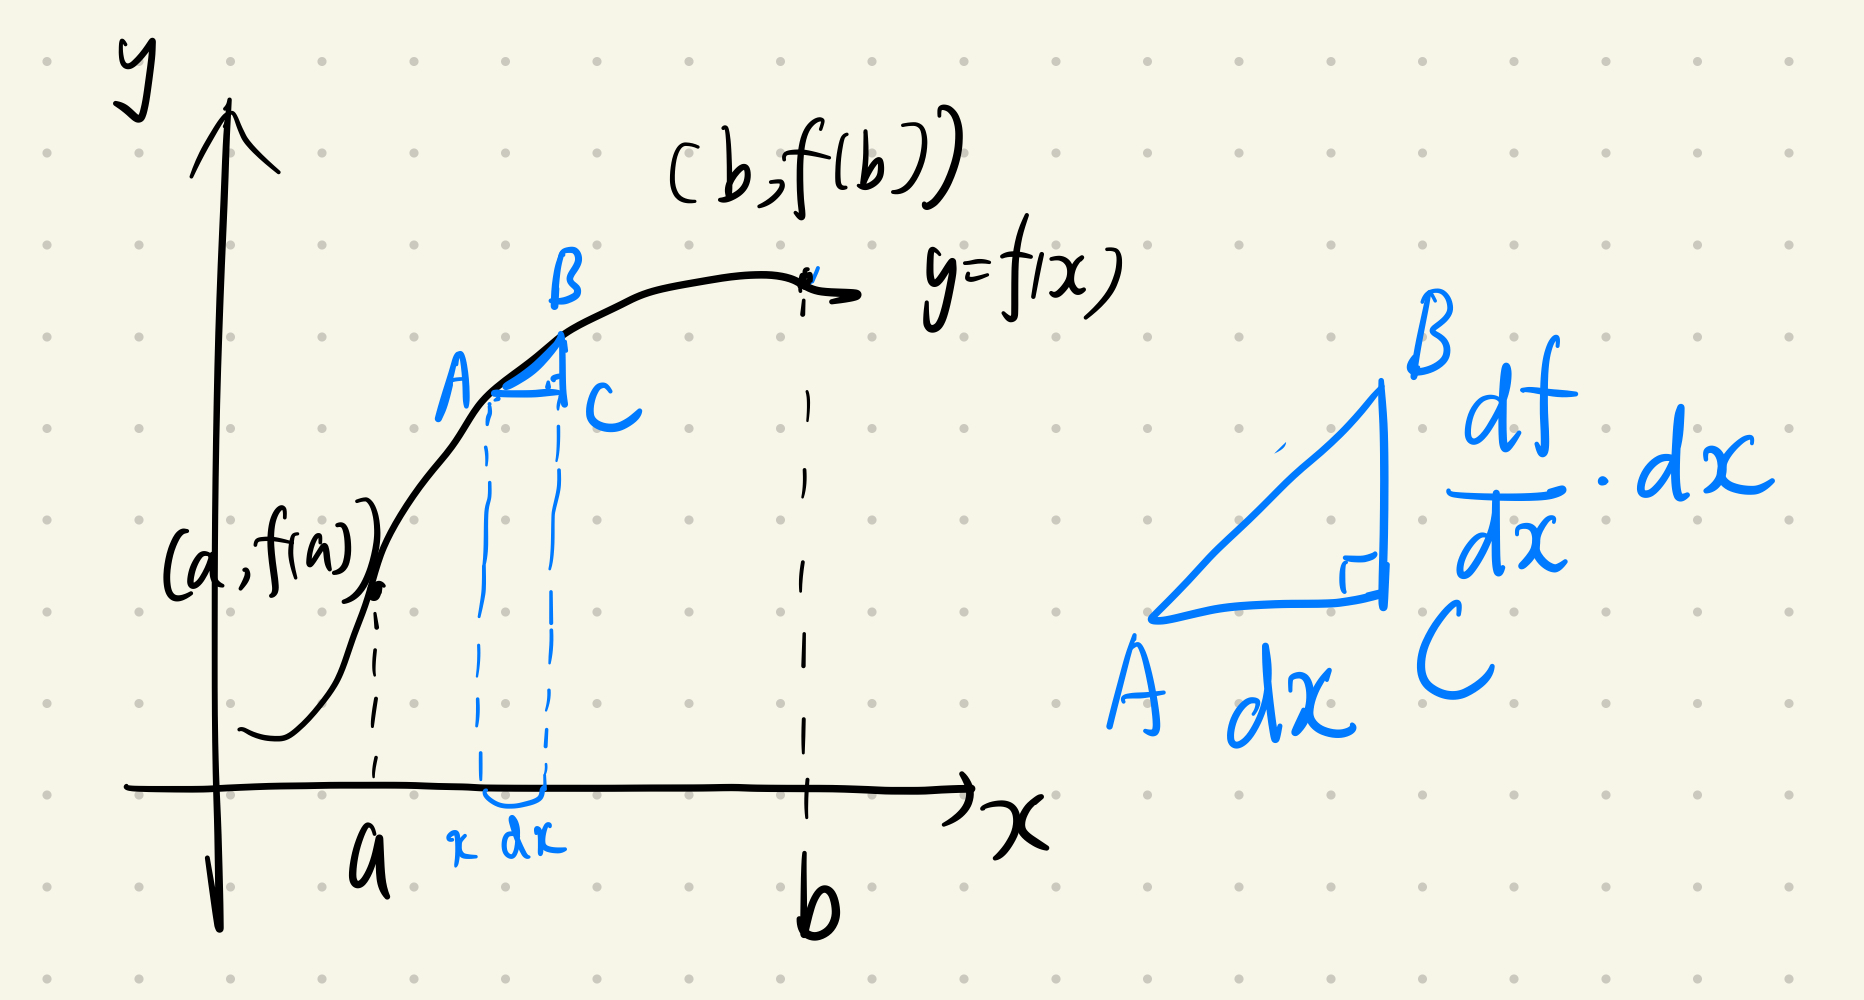
\includegraphics[width = 0.8\textwidth]{figures/chap 07/arc_length.png}
\end{figure}

As with previously where we broke up the area of interest into small strips of rectangles, here we break up the arc into small segments, shown as $\overline{AB}$ here.  As long as we can express $\overline{AB}$ as something shaped like $g(x)dx$, we can evaluate the arc length between $(a, f(a))$ and $(b, f(b))$ with the definite integral $\int_a^b g(x)~dx$.  

To find $g(x)$, we look at the right triangle $ABC$, magnified in the right panel of the graph above.  Given point $A$, point $B$ was constructed by taking an increment in $x$-coordinate by the differential $dx$, so we have $\overline{AC} = dx$.  The segment $\overline{BC}$ would then be the change in $f$ after the $x$-coordinate increment, which is the differential $df$ and can be alternatively written as $\frac{df}{dx}\cdot dx$.  Then, from the Pythagorean theorem:
\[\overline{AB} = \sqrt{\overline{AC}^2+\overline{BC}^2} = \sqrt{(dx)^2 + \Big(\frac{df}{dx}dx\Big)^2} = \sqrt{1 + \Big(\frac{df}{dx}\Big)^2}dx\]
Therefore, we have $g(x) = \sqrt{1 + \Big(\frac{df}{dx}\Big)^2}$, and the arc length is
\[S = \int_a^b \sqrt{1 + \Big(\frac{df}{dx}\Big)^2}dx\]
Let us try to evaluate a few arc lengths with our new formula:
\begin{eg}[]{eg: arc_length}
    Find the following arc lengths
    \begin{enumerate}[a)]
        \item The arc length of $y = \sqrt{1-x^2}$ between $x = -1$ and $x = 1$
        \item The arc length of $y = x^{3/2}$ between $x = 0$ and $x = 4$
        \item The arc length of $y = \ln(\sec x)$ between $x = \pi/6$ and $x = \pi/4$
    \end{enumerate}
\end{eg}

\begin{egsol}[]{egsol: arc_length}
    Find the following arc lengths
    \begin{enumerate}[a)]
        \item It is clear the $y = \sqrt{1-x^2}$ is the upper half of a circle centered at the origin with radius $1$, so our arc length should be half the circumference of a circle of radius $1$, which is $\pi$.  We can verify this by noting $\frac{dy}{dx} = -\frac{x}{\sqrt{1-x^2}}$, so the arc length should be
        \begin{align*}
            S &= \int_{-1}^1 \sqrt{1+\Big(\frac{dy}{dx}\Big)^2}~dx\\
            &= \int_{-1}^1 \sqrt{1+\Big(-\frac{x}{\sqrt{1-x^2}}\Big)^2}~dx\\
            &= \int_{-1}^1 \frac{1}{\sqrt{1-x^2}}~dx\\
            &= \arcsin x\Big]_{-1}^1 = \frac{\pi}{2} - \Big(-\frac{\pi}{2}\Big) = \pi
        \end{align*}
        where is identical to what we have predicted.
        \item Since $\frac{dy}{dx} = \frac{d x^{3/2}}{dx} = \frac{3}{2} \sqrt{x}$, the arc length can be evaluated by
        \begin{align*}
            S &= \int_0^4\sqrt{1+\Big(\frac{dy}{dx}\Big)^2}~dx\\
            &= \int_0^4\sqrt{1+\big(\frac{3}{2}\sqrt{x}\big)^2}~dx\\
            &= \int_0^4\sqrt{1+\frac{9}{4}x}~dx
        \end{align*}
        Now let $u = 1+\frac{9}{4}x$, so that $du = \frac{9}{4}dx$.  In addition, for the integration limits, when $x = 4$, $u = 10$; when $x = 0$, $u = 1$.  Therefore we have
        \begin{align*}
            S &= \int_0^4\sqrt{1+\frac{9}{4}x}~dx\\
            &=\frac{4}{9} \int_0^4\sqrt{1+\frac{9}{4}x}~\Big(\frac{9}{4}dx\Big)\\
            &=\frac{4}{9}  \int_1^10\sqrt{u}~du\\
            &= \frac{4}{9}\cdot \frac{2}{3}u^{3/2}\Big]_1^10 = \frac{8}{27}(10\sqrt{10}-1)
        \end{align*}
        \item Since $\frac{dy}{dx} = \frac{d \ln(\sec x)}{dx} = \tan x$, the arc length can be evaluated by
        \begin{align*}
            S &= \int_{\pi/6}^{\pi/4}\sqrt{1+\Big(\frac{dy}{dx}\Big)^2}~dx\\
            &= \int_{\pi/6}^{\pi/4}\sqrt{1+\tan^2 x}~dx\\
            &= \int_{\pi/6}^{\pi/4} \sec x~dx\\
            &= \ln|\sec x + \tan x|\big]_{\pi/6}^{\pi/4}\\
            &= \ln|\sqrt{2} + 1| - \ln|\frac{2}{\sqrt{3}}+\frac{1}{\sqrt{3}}| = \ln \frac{\sqrt{2}+1}{\sqrt{3}}
        \end{align*}
    \end{enumerate}
\end{egsol}

\begin{ex}[]{ex: arc_length}
    Find the arc length of $y = x^2$ between $x = 0$ and $x = 1/2$
\end{ex}

\begin{exsol}[]{exsol: arc_length}
    Since $\frac{dy}{dx} = \frac{dx^2}{dx} = 2x$, the arc length can be evaluated by
    \[S = \int_0^{1/2} \sqrt{1+\Big(\frac{dy}{dx}\Big)^2}~dx = \int_0^{1/2} \sqrt{1+(2x)^2}~dx\]
    To eliminate the square root, we let $2x = \tan \theta$, so that $dx = \frac{1}{2}\sec^2 \theta d \theta$.  For the limits of integration, when $x = 1/2$, $\theta = \arctan 1 = \frac{\pi}{4}$; when $x = 0$, $\theta = \arctan 0 = 0$.  Therefore we have
    \[S = \int_0^{1/2} \sqrt{1+(2x)^2}~dx = \int_0^{\pi/4} \sqrt{1+\tan^2\theta}~\frac{1}{2}\sec^2\theta d\theta= \frac{1}{2} \int_0^{\pi/4} \sec^3\theta d\theta\]
    To evaluate $\int_0^{\pi/4} \sec^3\theta d\theta$, we will need to use integration by parts where $u = \sec \theta, dv/d\theta = \sec^2 \theta$, so that $du/dx = \sec\theta \tan\theta, v = \tan \theta$:
    \begin{align*}
        \int_0^{\pi/4} \sec^3\theta d\theta &= \int_0^{\pi/4} \sec \theta \cdot \sec^2 \theta~d\theta\\
        &= \sec \theta \tan \theta\big]_0^{\pi/4} - \int_0^{\pi/4} \sec\theta \tan\theta \cdot \tan\theta d\theta\\
        &= \sec \theta \tan \theta\big]_0^{\pi/4} - \int_0^{\pi/4} \sec\theta \tan^2\theta d\theta\\
        &= \sec \theta \tan \theta\big]_0^{\pi/4} - \int_0^{\pi/4} \sec\theta (\sec^2\theta -1) d\theta\\
        &= \sec \theta \tan \theta\big]_0^{\pi/4} - \int_0^{\pi/4} \sec^3\theta d\theta + \int_0^{\pi/4} \sec\theta~d\theta\\
        &= \sec \theta \tan \theta\big]_0^{\pi/4} + \ln|\sec\theta + \tan\theta|\big]_0^{\pi/4} - \int_0^{\pi/4} \sec^3\theta d\theta\\
    \end{align*}
    Now both sides of the equation has the definite integral of $\int_0^{\pi/4}\sec^3\theta~d\theta$, so we aggregate them to the left:
    \begin{align*}
        &2\int_0^{\pi/4}\sec^3\theta~d\theta\\
        = &\Big(\sec\frac{\pi}{4}\tan\frac{\pi}{4}-\sec 0 \tan 0\Big) + \Big(\ln|\sec\frac{\pi}{4}+\tan\frac{\pi}{4}|-\ln|\sec 0 + \tan 0|\Big)\\
        = & (\sqrt{2} -0)+ (\ln|\sqrt{2}+1|-\ln|1|) = \sqrt{2}+\ln(\sqrt{2}+1)
    \end{align*}
    Therefore, we have
    \[ S= \frac{1}{2}\int_0^{\pi/4}\sec^3\theta~d\theta = \frac{1}{4} \cdot 2\int_0^{\pi/4}\sec^3\theta~d\theta = \frac{1}{4}[\sqrt{2}+\ln(\sqrt{2}+1)]\]
\end{exsol}

\section{Volume and surface area for solids of revolution}

In the previous section we've seen that definite integrals can help us evaluate the area under the curve, area between two curves, and the arc length of a curve.  We arrived at these definite integrals by slicing the area or arc length into pieces that can be expressed with $g(x)dx$, and then integrating them back to obtain the area or arc length of interest.  In this section, we will show that definite integrals can also help us evaluate the volume and surface area for solids of revolution, which are solids that has at least one axis of rotational symmetry, eg. a ball, an ellipsoid or a cone. 

Suppose a solid of revolution can be created by taking a curve $y = f(x)$ from $x = a$ to $x = b$ and rotating it about the $x$-axis.  For example, in the following graph, we have a clay pot-shaped solid that is rotationally symmetric along the $x$-axis.  Then, analogous to our previous approach, to evaluate the volume of the solid, we can slice the solid along the $x$-axis to get a series of thin disks.  If the volume of these disks can be expressed in the form of $g(x)dx$, then we can integrate $g(x)$ along the $x$-axis from $x=a$ to $x=b$ to get our desired volume.  

\begin{figure}[ht]
    \centering
    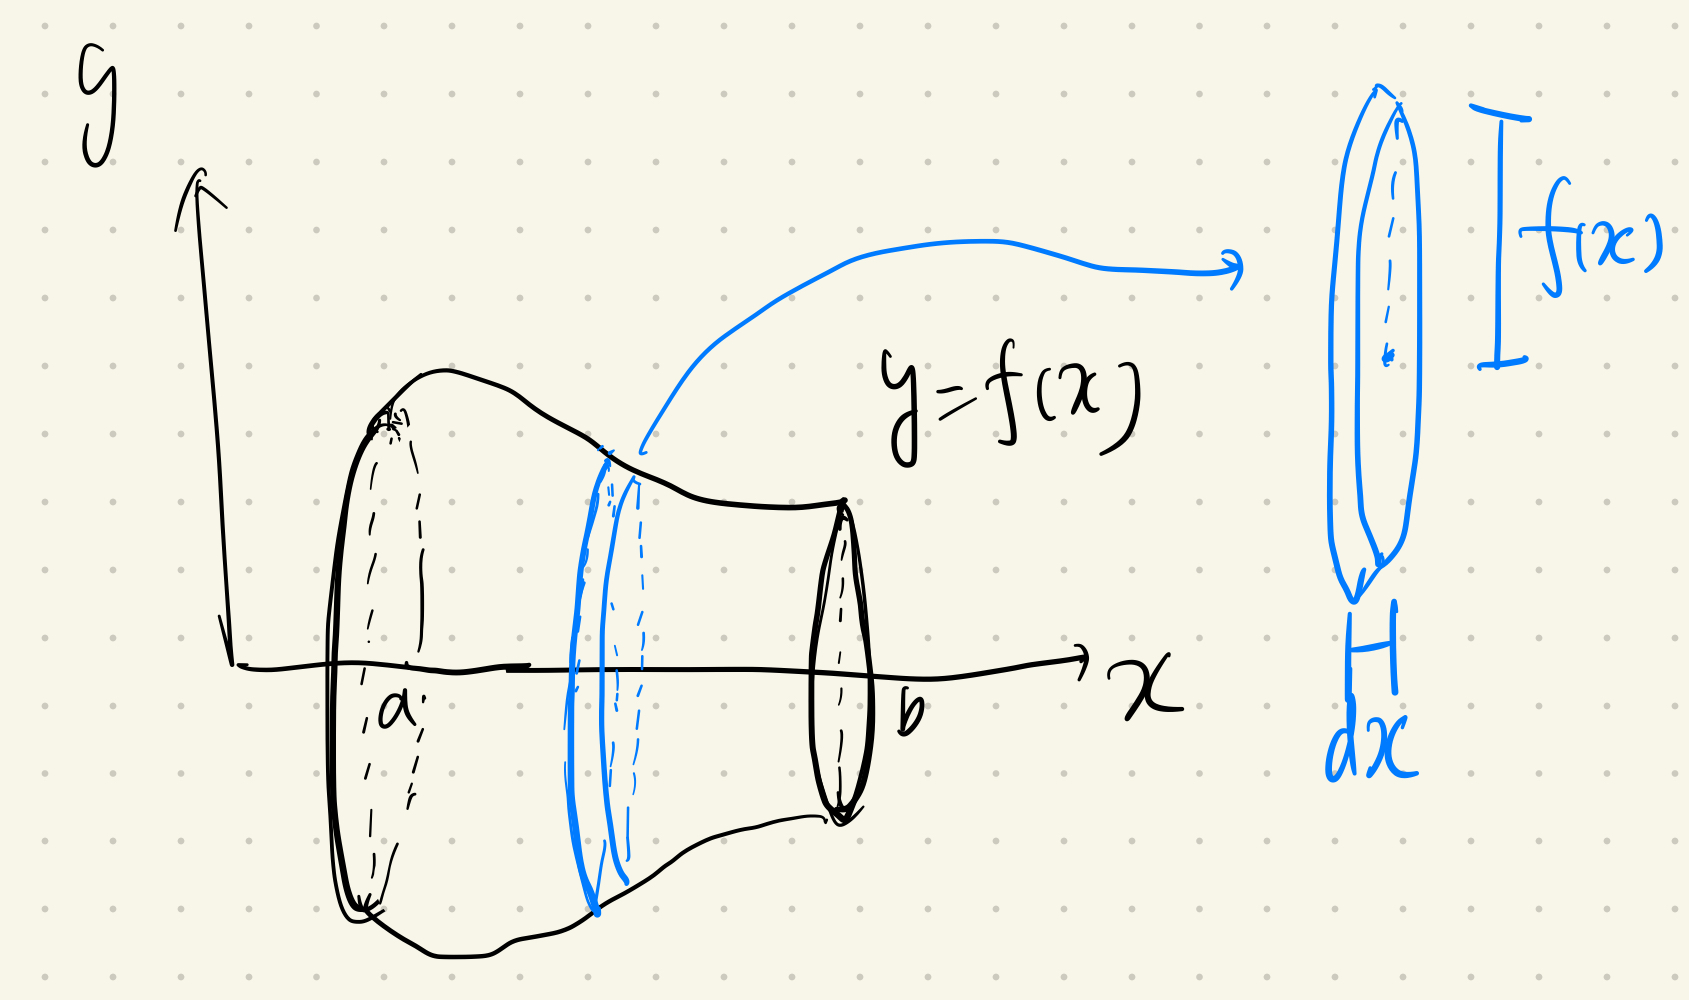
\includegraphics[width = 0.6\textwidth]{figures/chap 07/revolution_vol.png}
\end{figure}

The right panel of the graph above shows one slice of the thin disk.  As the disk gets thinner and thinner, it is approaching the shape of the cylinder.  Therefore, to evaluate the volume of the disk, we need to know the area of its base and its width.  For the width, since we are slicing along the $x$-axis, the width of the disk would be the differential $dx$.  For the area of its base, since this is a rotational solid, the section of each disk would be a circle, with its radius as $f(x)$ since we are rotating $y = f(x)$ around the $x$-axis.  Therefore, the area of the base should be $\pi (f(x))^2$, and the volume of the disk is then $\pi (f(x))^2 dx$.  At last, the volume for the solid of revolution would be
\[V = \int_a^b \pi (f(x))^2~dx\]

\begin{figure}[ht]
    \centering
    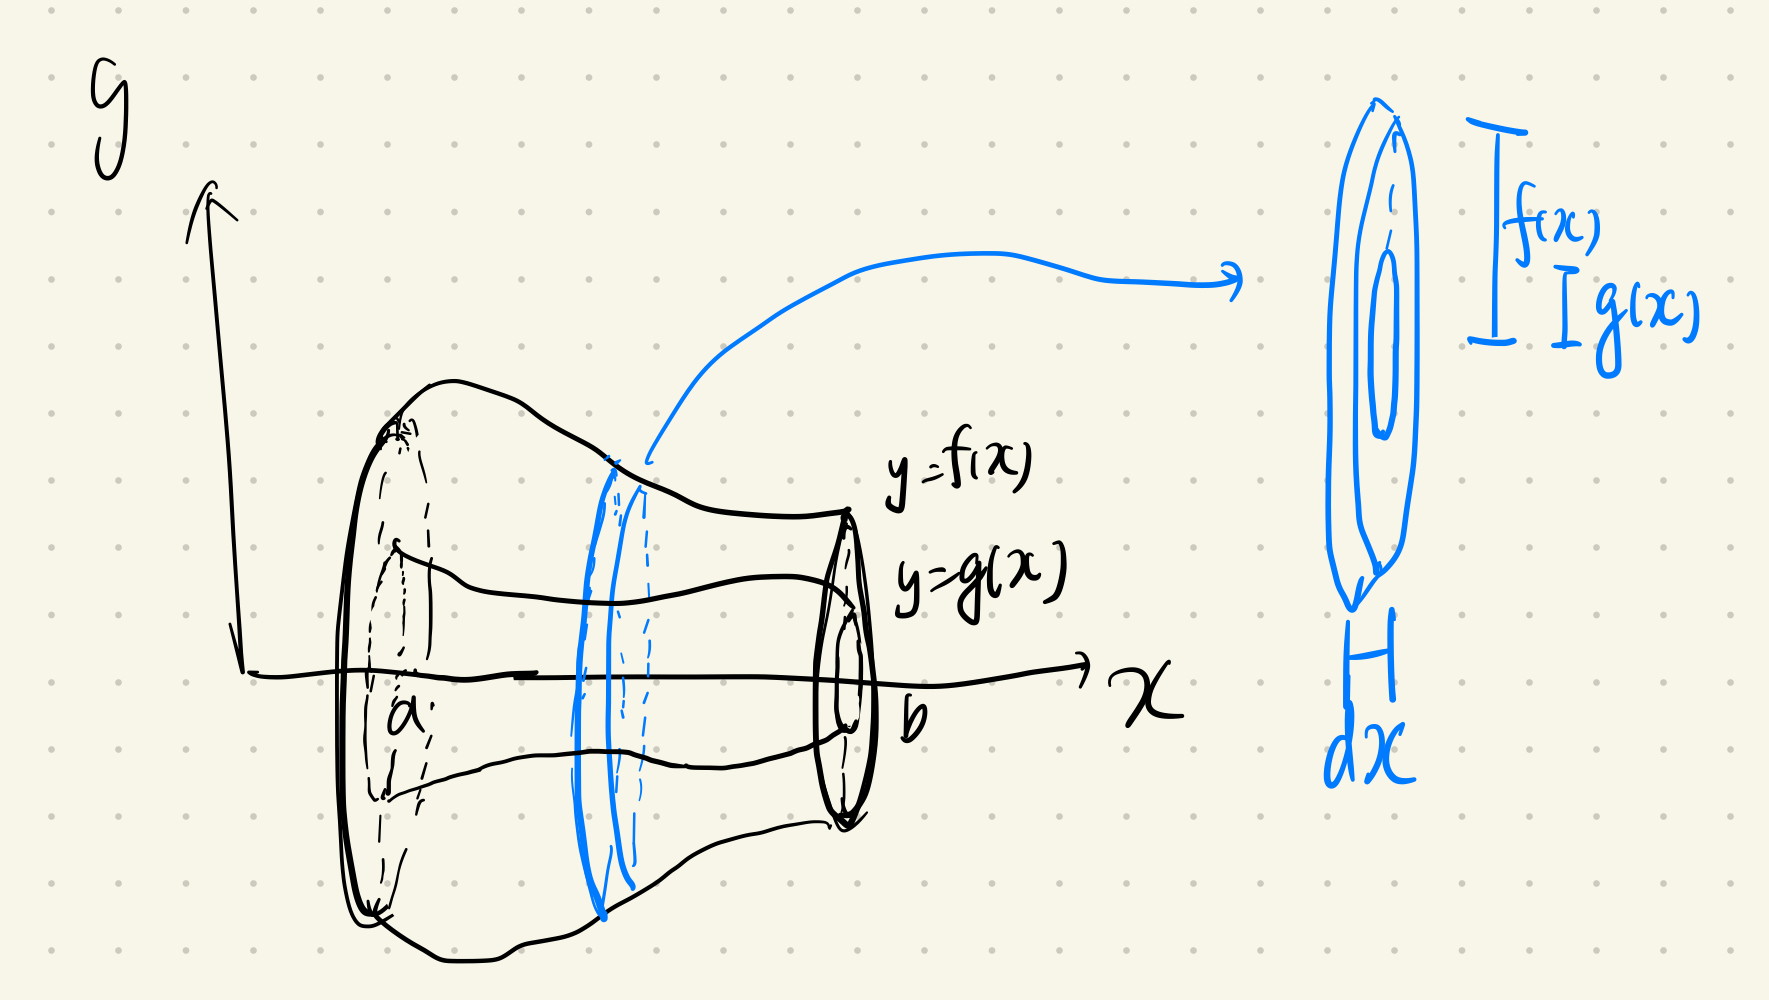
\includegraphics[width = 0.6\textwidth]{figures/chap 07/revolution_vol_ring.png}
\end{figure}

In the case where the solid revolution is formed by rotating the area between two curves along the $x$-axis, such as the graph above where the area between $y=f(x)$ and $y=g(x)$ are rotated, then volume of the thin disks, which is now a thing ring, would be $\pi [(f(x))^2-(g(x))^2] dx$ instead since we have to subtract the volume of the inner cylinder from the outer cylinder.  Therefore, the volume for the hallow solid of revolution would be 
\[V = \int_a^b \pi [(f(x))^2-(g(x))^2]~dx\]

Here our method slices the solid of revolution into disks or rings, depending on if the solid is hallow inside.  Therefore, this method is sometimes termed as the \textit{method of disks} or \textit{method of rings}.  We now show how they work with some examples:

\begin{eg}[]{eg: rev_solid_vol_ring}
    Verify the volume of the following solids using the method of disks
    \begin{enumerate}[a)]
        \item A ball of radius $r$ has volume $\frac{4}{3}\pi r^3$.
        \item A cone of height $h$ and radius of base $r$ has volume $\frac{1}{3}\pi r^2 h$.
    \end{enumerate}
\end{eg}

\begin{egsol}[]{egsol: rev_solid_vol_ring}
    \begin{enumerate}[a)]
        \item If we put a semi-circle of radius $r$ on the $x$-axis and rotate it about the axis, then we would get a ball of radius $r$ as the solid of revolution.  Therefore, as shown in the graph below, we can let $y = f(x) = \sqrt{r^2-x^2}$, which represents a semi-circle of radius $r$ with center at the origin, and evaluate the volume for the solid of revolution from $x = -r$ to $x = r$, which yields
        \begin{center}
            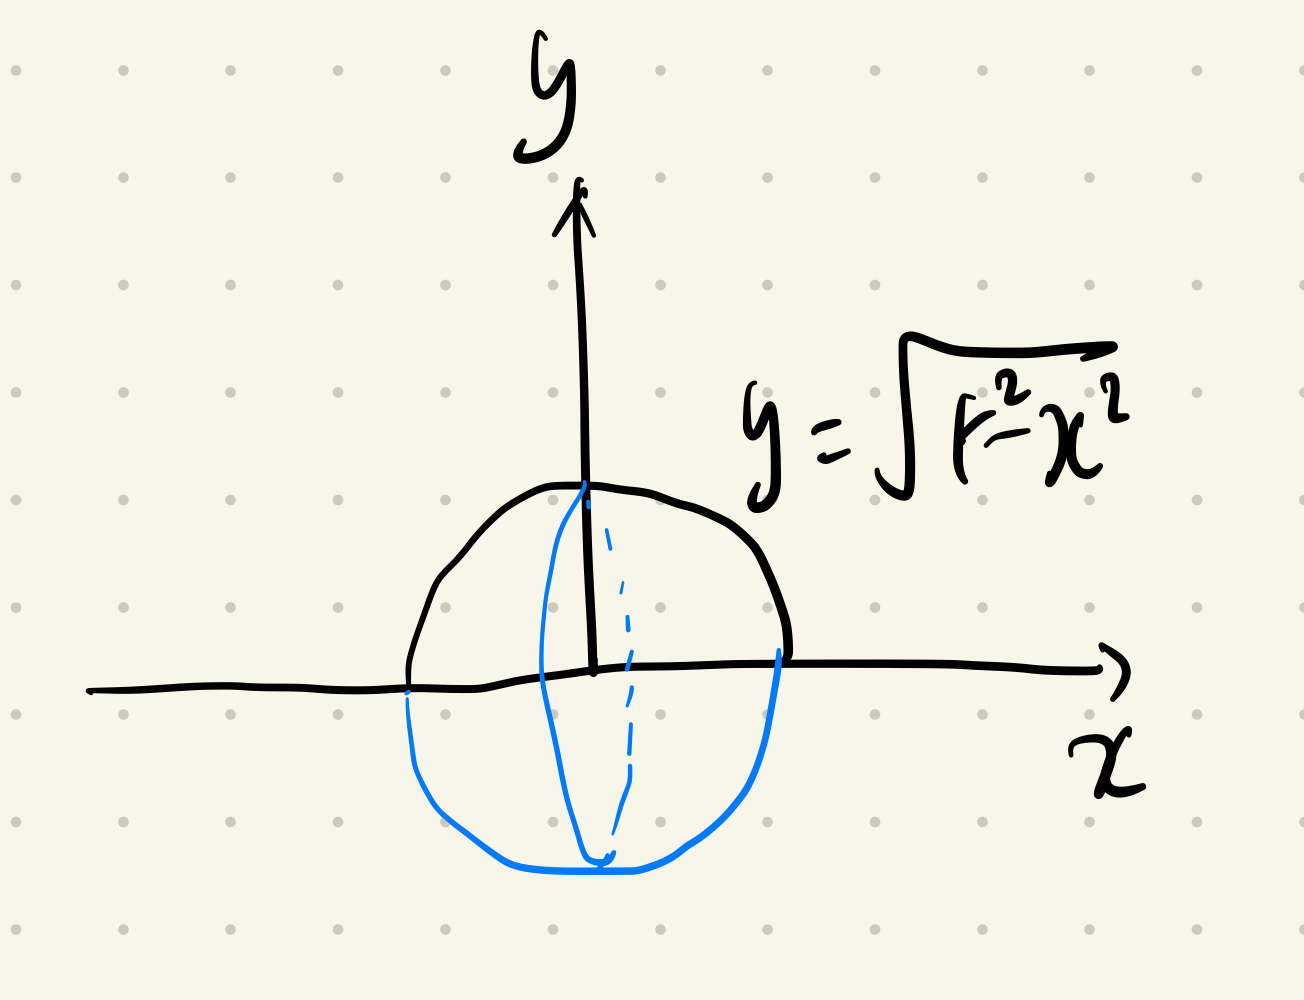
\includegraphics[width = 0.3\textwidth]{figures/chap 07/rev_solid_ball.png}
        \end{center}
        \begin{align*}
            V &= \int_{-r}^r \pi (\sqrt{r^2-x^2})^2~dx\\
            &= \int_{-r}^r (\pi r^2 - \pi x^2) ~dx\\
            &= \pi r^2 x - \frac{1}{3} \pi x^3\big]{-r}^r\\
            &= (\pi r^2 \cdot r - \frac{1}{3} \pi r^3) - ((\pi r^2 \cdot (-r) - \frac{1}{3} \pi (-r)^3))\\
            &= \big(1-\frac{1}{3} + 1 - \frac{1}{3}\big)r^3 = \frac{4}{3}\pi r^3
        \end{align*}
        \item As shown in the following graph, if we rotate a right angle triangle with base $h$ and height $r$ about the $x$-axis, we would get a cone described by the problem.  The hypotenuse of the triangle would have a slope of $r/h$, so its equation would be $y = (r/h)x$.  We can thus evaluate the volume for the solid of revolution from $x = 0$ to $x = h$ for $y = (r/h) x$, which yields
        \begin{center}
            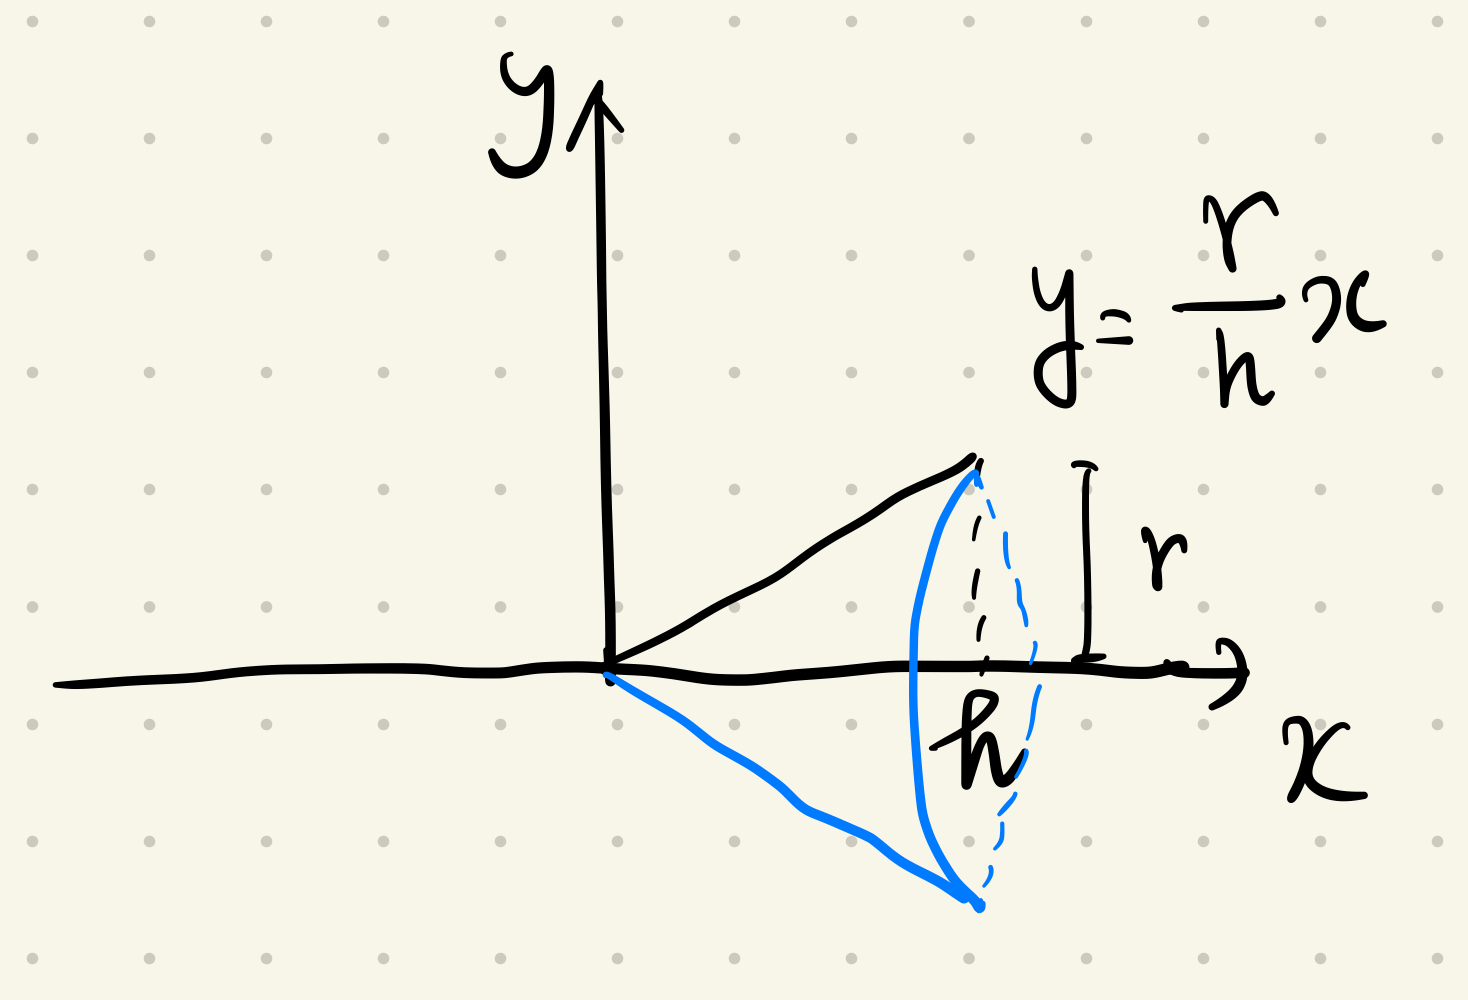
\includegraphics[width = 0.3\textwidth]{figures/chap 07/rev_solid_cone.png}
        \end{center}
        \begin{align*}
            V &= \int_0^h \pi \big(\frac{r}{h}x)^2~dx\\
            &= \int_0^h \pi \frac{r^2}{h^2} x^2~dx\\
            &= \pi \frac{r^2}{h^2} \cdot \frac{1}{3}x^3 \Big]_0^h\\
            &= \pi \frac{r^2}{h^2} \cdot \frac{1}{3}h^3 = \frac{1}{3} \pi r^2 h
        \end{align*}
    \end{enumerate}
\end{egsol}

\begin{ex}[]{ex: rev_solid_vol_ring}
    Find the volume of the solid constructed by revolving the area enclosed by $y = x$ and $y = \sqrt{x}$ around the $x$-axis.
\end{ex}

\begin{exsol}[]{exsol: rev_solid_vol_ring}
    \begin{center}
        \includegraphicsex{width = 0.65\textwidth, draft}{width = 0.65\textwidth}{figures/chap 07/method_of_rings.png}
    \end{center}
    As shown in the graph above, the range of $x$-coordinate for the area enclosed by $y=x$ and $y=\sqrt{x}$ is $x=0$ to $x=1$.  When this area is revolved around the axis to form a solid of revolution, we can slice the solid along the $x$-axis and get rings shaped as the right hand side, with width $dx$ and area of the base made up of two concentric circles, the larger one with radius $\sqrt{x}$ (since $\sqrt{x} \ge x$ within $x \in [0, 1]$) and the smaller one with radius $x$.  Therefore, the ring slice has volume
    \[\pi [(\sqrt{x})^2 - x^2] dx = \pi (x - x^2) dx\]
    and the volume the whole solid can be found by integrating the volume of the ring slices and letting $x$ go from $0$ to $1$:
    \[\int_0^1 \pi (x - x^2) dx = \pi \int_0^1 (x - x^2) dx = \pi \Big(\frac{1}{2}x^2 - \frac{1}{3}x^3\Big)\Big]_0^1 = \pi \Big(\frac{1}{2}-\frac{1}{3}) = \frac{\pi}{6}\]
\end{exsol}

\begin{ex}[]{ex: rev_solid_vol_y}
    Find the volume of the solid constructed by revolving the area between the $y$-axis and the curve of $y = x^2$ from $x = 0$ to $x = 2$ around the $y$-axis. 
\end{ex}

\begin{exsol}[]{exsol: rev_solid_vol_y}
    \begin{center}
        \includegraphicsex{width = 0.6\textwidth, draft}{width = 0.6\textwidth}{figures/chap 07/method_of_disks_y.png}
    \end{center}
    In this problem, the solid of revolution is not revolving about the $x$-axis but instead the $y$-axis, so we cannot directly use the formula shown in the previous text.  However, we can still use the method of disks, but now as shown in the graph, we need to slice the solid of revolution along the $y$-axis instead of the $x$-axis to get slices of disks shaped as shown on the right.  The height of the disk would be $dy$, and when the $y$-coordinate of the disk is denoted as $y$, the radius of the disk would be $\sqrt{y}$ since $(\sqrt{y}, y)$ would be on the curve.  Therefore, the volume of the slice of disk is
    \[\pi (\sqrt{y})^2 dy = \pi y~dy\]
    and the volume of the whole solid can be evaluated by integrating the volume of the disks from $y = 0^2 = 0$ to $y = 2^2 = 4$
    \[\int_0^4 \pi y~dy = \pi \int_0^4 y~dy = \pi \Big(\frac{1}{2}y^2\Big)\Big]_0^4 = \frac{1}{2}\cdot 16 = 8\]
\end{exsol}

In the previous exercise, we found the volume of a solid revolving about the $y$-axis with the method of disks.  This approach worked since we could express the radius of each disk with $y$ by solving for $x$ in $y = x^2$.  However, in the case where the curve revolving the $y$-axis is more complex, eg. $y =  e^x - x$, we cannot solve for $x$ anymore, so the method of disks does not work.

\begin{figure}[ht]
    \centering
    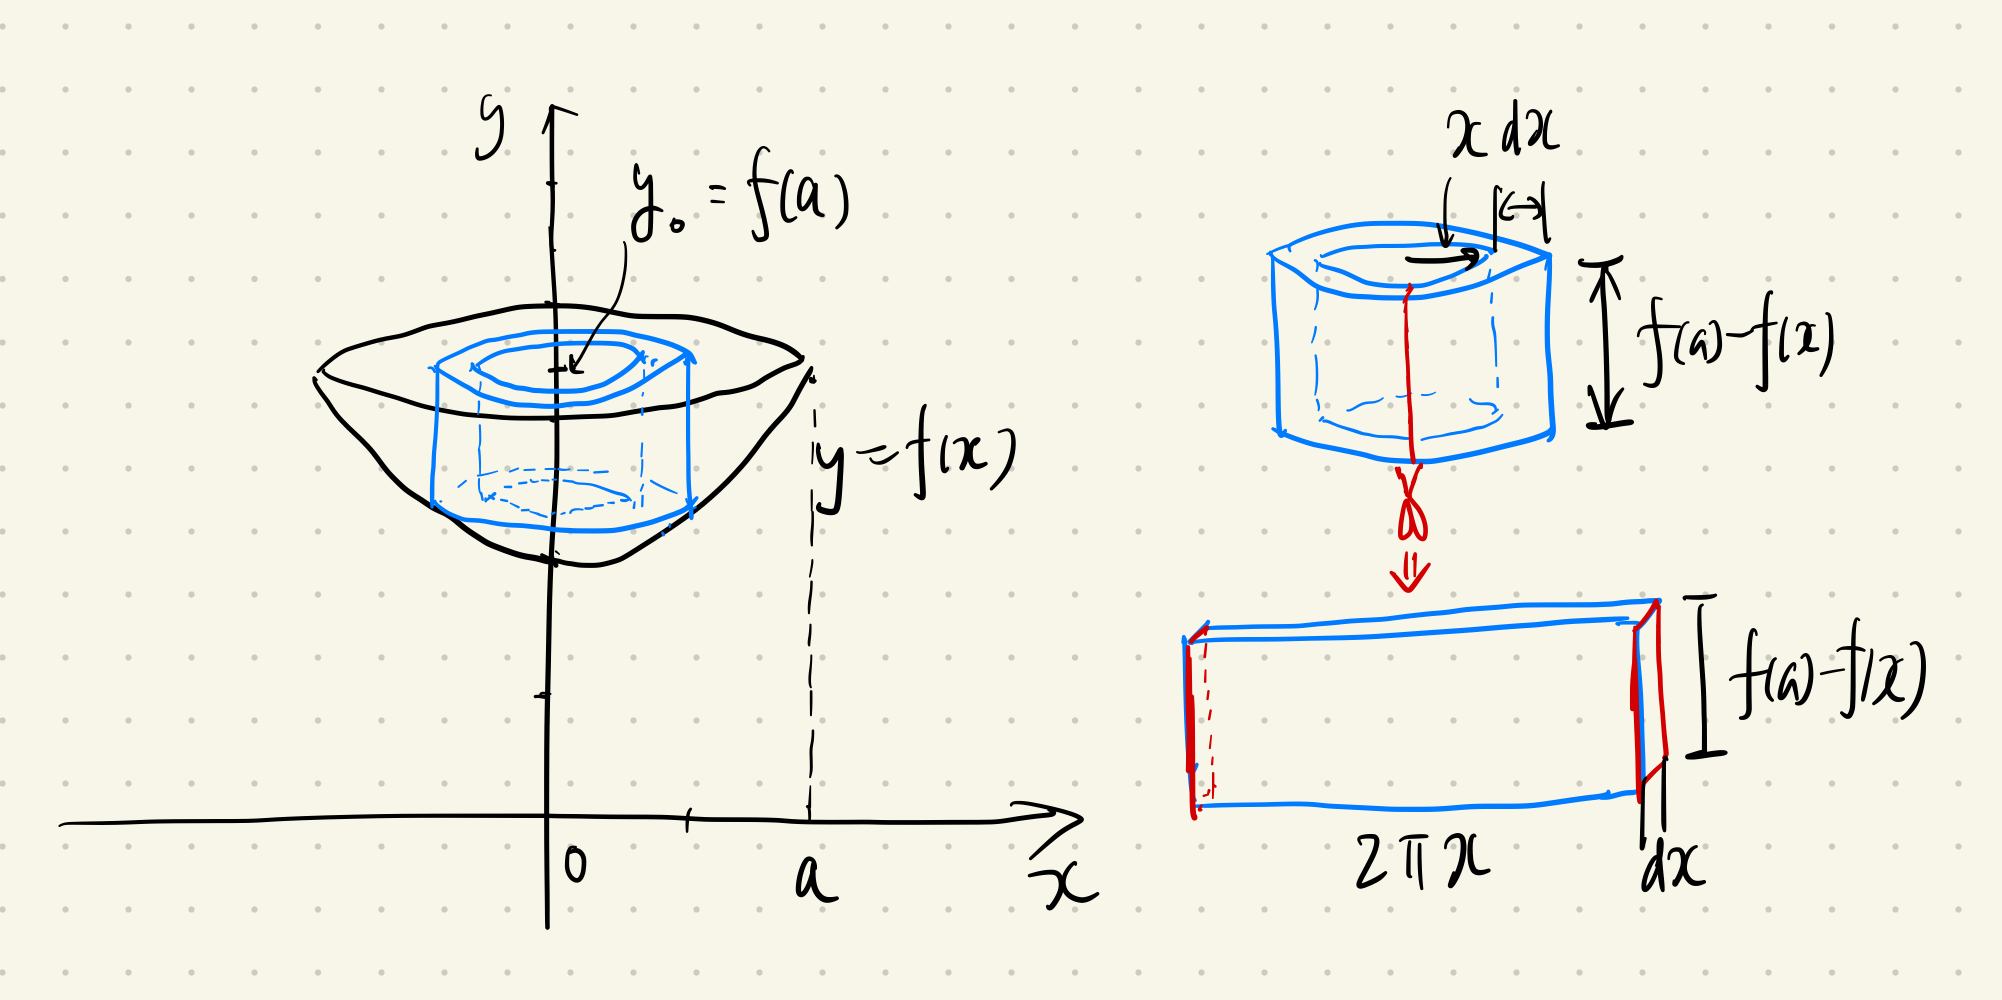
\includegraphics[width = 0.9\textwidth]{figures/chap 07/method_of_shells.png}
\end{figure}

\medskip
Aside from the method of disks, we still have another trick up our sleeves that can help us evaluate the volume of a solid of revolution.  Suppose we would like to find the volume of the solid constructed by revolving the area between the $y$-axis and $y = f(x)$ from $x = 0$ to $x = a$ around the $y$-axis.  In the method of disks, we would slice up the solid along the $y$-axis so that each slice is a thin disk.  However, we can alternatively slice up the solid into thin cylindrical shells with inner radius $x$ and thickness, as shown in the graph above.  The height of the shells depends on how the function behaves, but in this case it is $f(a)-f(x)$.  The solid can then be seen as a collection of thin shells with inner radius $x$ ranging from $0$ to $a$.  To derive the volume of each thin shell, we can cut it open as in the right panel and we would get a thin sheet with thickness $dx$, width $2 \pi x$ and height $f(a) - f(x)$.  Therefore, the volume of the thin shell is
\[2\pi x (f(a)-f(x))~dx\]
and the volume of the solid of revolution can be found by the integral
\[V = \int_0^a 2\pi x (f(a)-f(x))~dx\]
Since this method slices the solid of revolution into shells, it is terms as the \textit{method of shells}.  We now show how it works with the following example:

\begin{eg}[]{eg: rev_solid_vol_y_shell}
    Find the volume of the solid constructed by revolving the area between the $x$-axis and the curve of $y = e^x - x$ from $x = 0$ to $x = 1$ around the $y$-axis. 
\end{eg}

\begin{egsol}[]{exsol: rev_solid_vol_y_shell}
    \begin{center}
        \includegraphicsex{width = 0.7\textwidth, draft}{width = 0.7\textwidth}{figures/chap 07/method_of_shells_eg.png}
    \end{center}

    \medskip
    If we sketch out the solid, it is shaped like a cylinder with a bowl-like dent on the top, as shown in the graph above.  If we try to use the method of disks / rings to solve for it volume, then we will have to slice up the solid along the $y$-axis.  The bottom part of the slices will be easy to tackle, since they are all disks of radius $1$.  However, when we get to the top part with the dent, we will get rings instead of disks, and the inner radius of the rings will not be tractable since we will have to solve for $x$ in $y = e^x - x$. 
    
    Since the method of disks / rings is not viable for this problem, we turn to the method of shells.  If we slice the solid into concentric thin shells with inner radius $x$ and thickness $dx$, then the height of the shells, from the graph, would be $e^x - x$.  Therefore, the volume of the shells would be $2 \pi x (e^x-x)~dx$, and the volume of the solid can be obtained by integrating the volume of shells with $x$ going from $0$ to $1$:
    \begin{align*}
        \int_0^1 2 \pi x (e^x-x)~dx &= 2\pi\Big[\int_0^1 xe^x~dx - \int_0^1 x^2~dx\Big]\\
        &= 2\pi\Big[xe^x\big]_0^1 - \int_0^1 e^x~dx - \int_0^1 x^2~dx\Big]\\
        &= 2\pi\Big[xe^x\big]_0^1 - e^x\big]_0^1 - \frac{1}{3}x^3\big]_0^1\Big] = 2\pi\Big[e - (e - 1) - \frac{1}{3}\Big] = \frac{4}{3}\pi
    \end{align*}
\end{egsol}

We have now known how to evaluate the volume for a solid of revolution using definite integrals.  A natural follow-up question is that how do we find the surface area for a solid of revolution.  The approach we are taking is basically the same as finding arc lengths, only that now we are not chopping the curve into small segments, but slicing the surface area into "onion rings" demonstrated below, where we are trying to find the surface area for the solid revolving $y = f(x)$ from $x = a$ to $x = b$ around the $x$-axis:

\begin{figure}[ht]
    \centering
    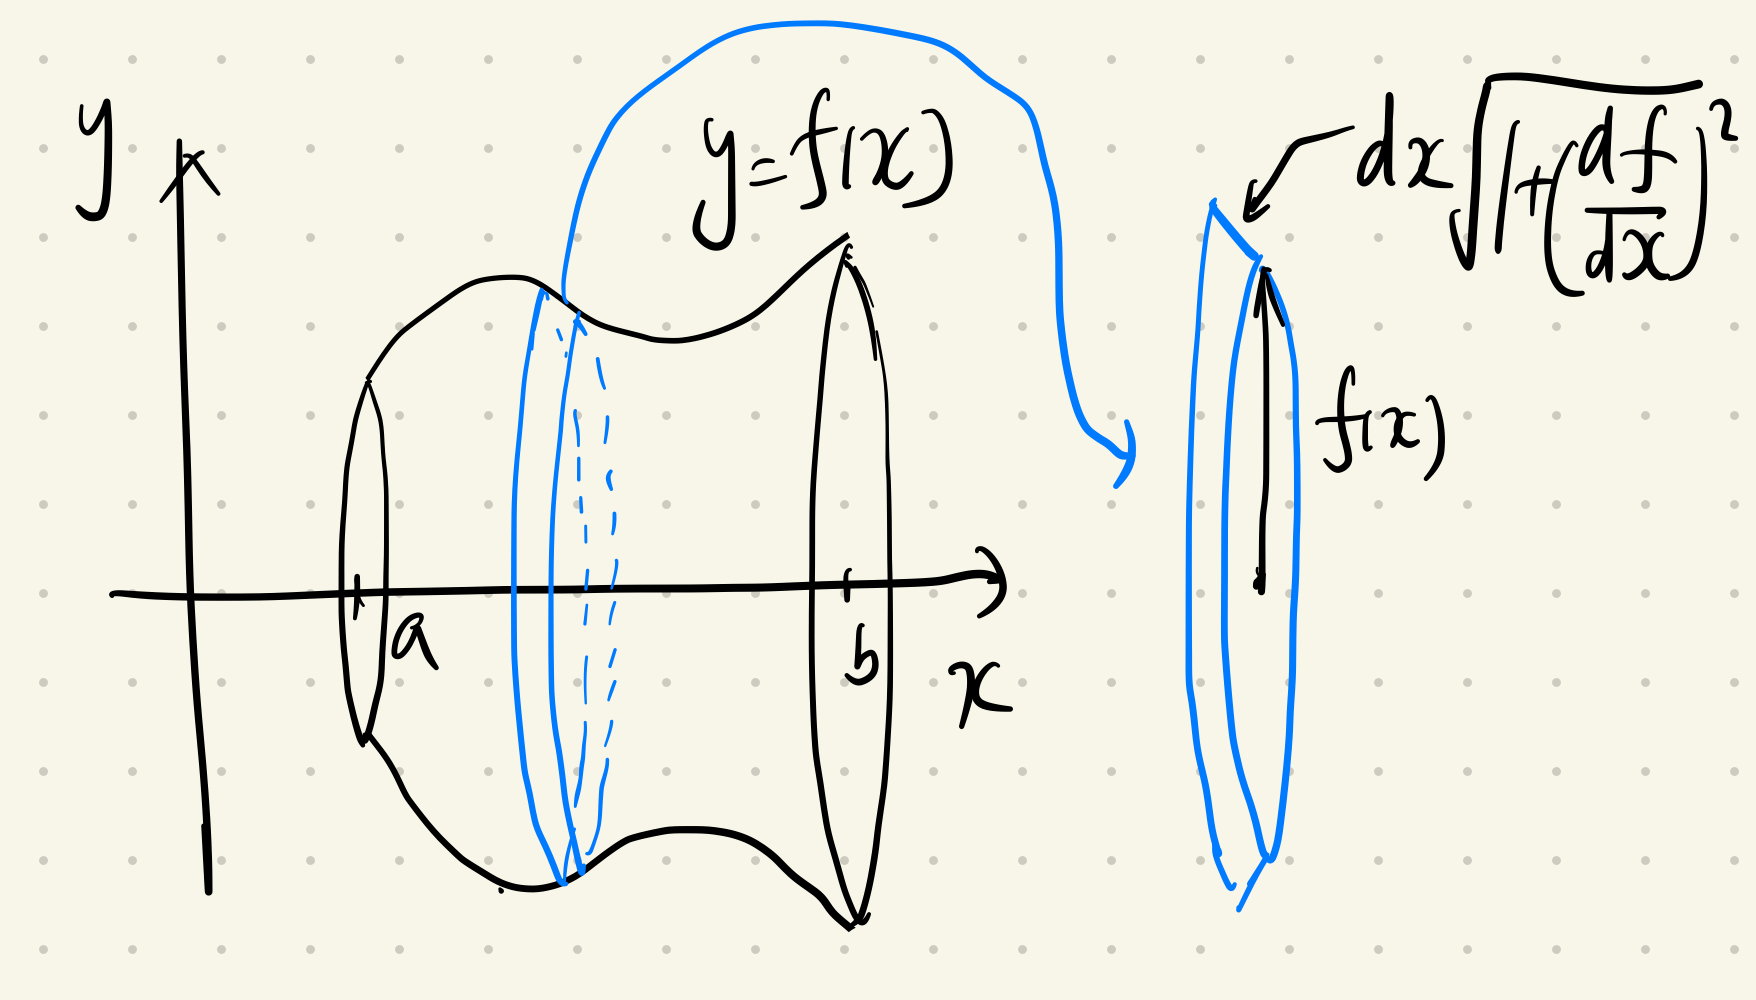
\includegraphics[width = 0.7\textwidth]{figures/chap 07/surface_area.png}
\end{figure}

here the slanted width of the ring is exactly the length of small segment in the derivation of arc lengths, so the width is also $\sqrt{1+(df(x)/dx)^2}~dx$.  Since this slanted width is revolved around the $x$-axis with radius $f(x)$ to form the surface of the solid, the surface area it sweeps through would be
\[2\pi f(x) \sqrt{1+\Big(\frac{df(x)}{dx}\Big)^2}~dx\]
Therefore, the surface area of the whole solid (excluding the left and right round caps by default) can be evaluated by integrating the surface area of the ring where $x$ goes from $a$ to $b$:
\[A = \int_a^b 2\pi f(x) \sqrt{1+\Big(\frac{df(x)}{dx}\Big)^2}~dx\]
We will end this section demonstrating how the surface area of balls and cones can also be evaluated using integrals.

\begin{eg}[]{eg: rev_solid_surf}
    Verify the surface area of the following solids
    \begin{enumerate}[a)]
        \item A ball of radius $r$ has surface area $4\pi r^2$.
        \item The lateral surface area of a cone of height $h$ and radius of base $r$ is $\pi r \sqrt{r^2+h^2}$.
    \end{enumerate}
\end{eg}

\begin{egsol}[]{egsol: rev_solid_surf}
    \begin{enumerate}[a)]
        \item As we have elaborate previously, a ball of radius $r$ can be constructed by revolving $y = f(x) = \sqrt{r^2-x^2}$ about the $x$-axis, as shown in the graph below. 
        \begin{center}
            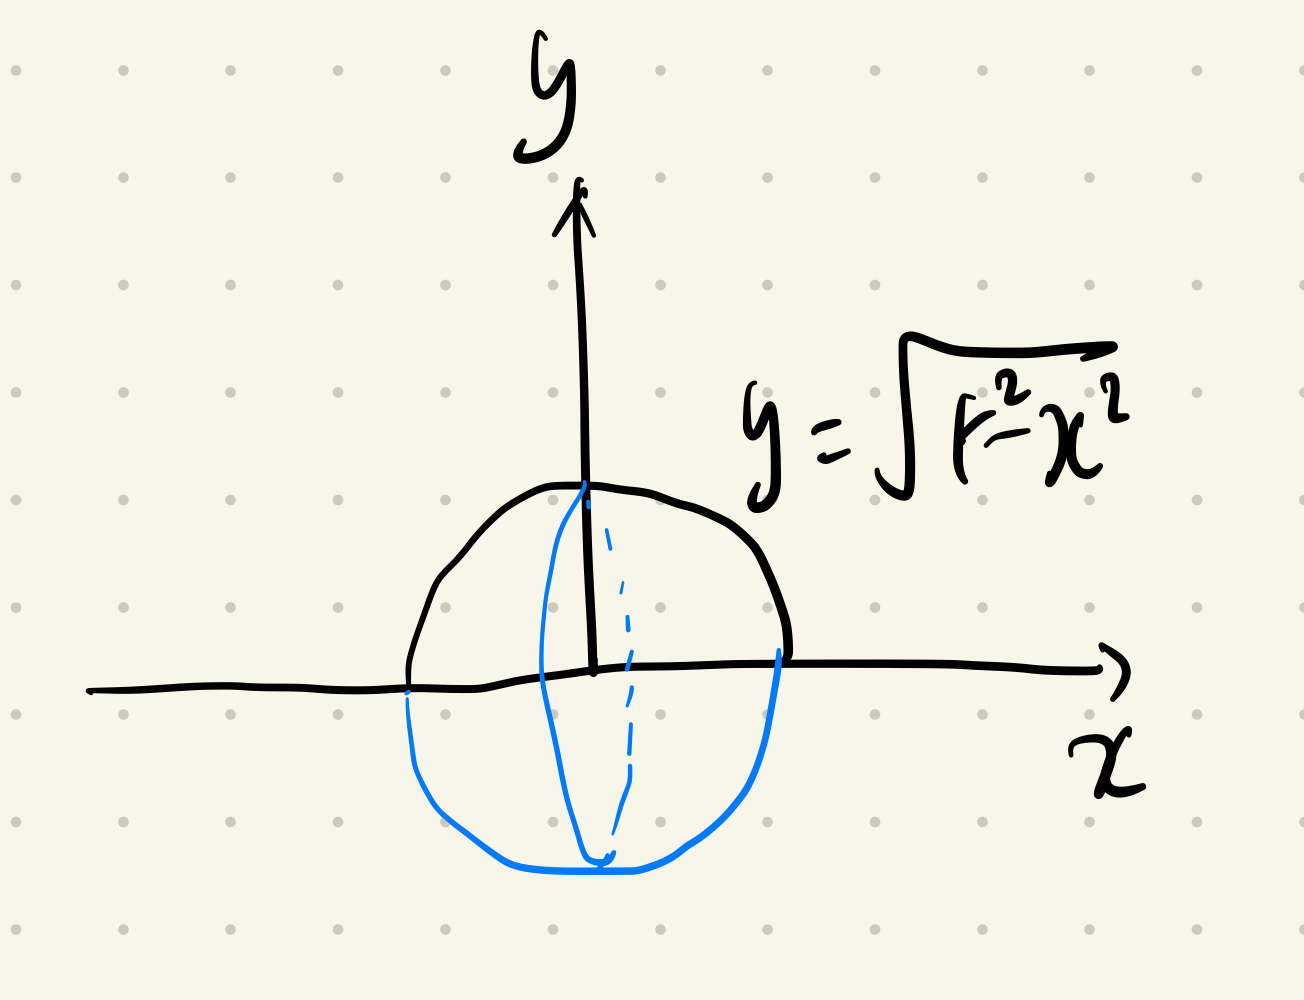
\includegraphics[width = 0.3\textwidth]{figures/chap 07/rev_solid_ball.png}
        \end{center}
        Therefore, we can use our formula to find the surface area of the ball:
        \begin{align*}
            A &= \int_{-r}^r 2 \pi f(x)\sqrt{1+\Big(\frac{df(x)}{dx}\Big)^2}~dx\\
            &= \int_{-r}^r 2 \pi \sqrt{r^2-x^2}\sqrt{1+\Big(\frac{-x}{\sqrt{r^2-x^2}}\Big)^2}~dx\\
            &= \int_{-r}^r 2 \pi \sqrt{r^2-x^2}\sqrt{\frac{r^2}{r^2-x^2}}~dx\\
            &= \int_{-r}^r 2 \pi r~dx = 2 \pi r x\big]_{-r}^r = 4 \pi r^2
        \end{align*}
        \item We have shown that if we revolve $y = f(x) = (r/h)x$ from $x = 0$ to $x = h$ around the $x$-axis, we would arrive at the cone for our problem, shown in the graph below:
        \begin{center}
            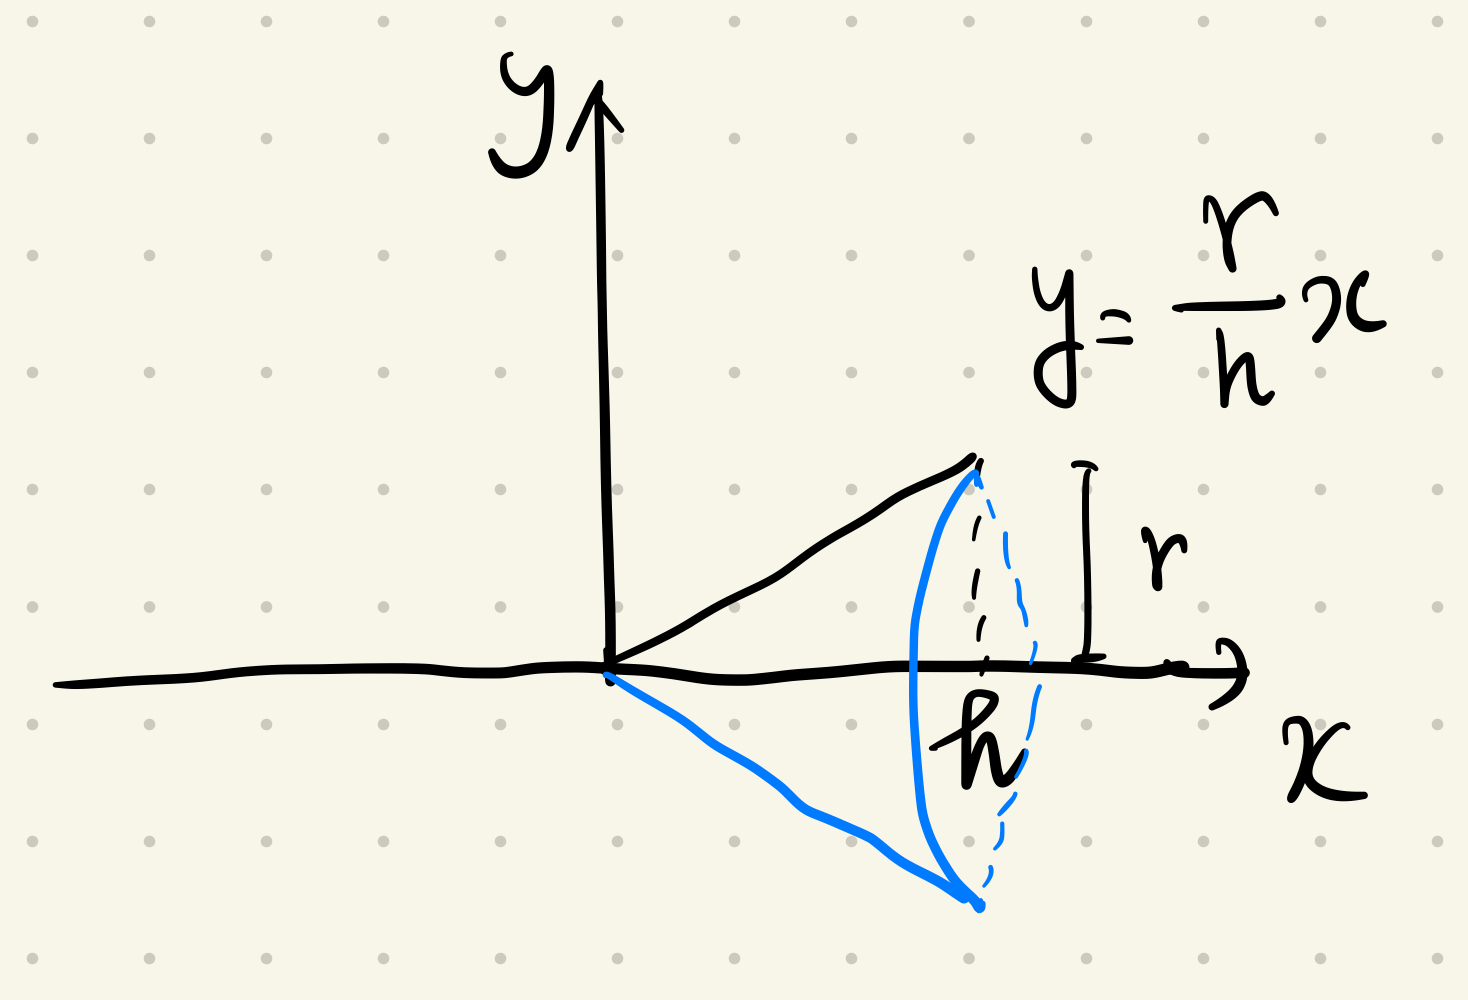
\includegraphics[width = 0.3\textwidth]{figures/chap 07/rev_solid_cone.png}
        \end{center}
        \allowdisplaybreaks
        Therefore, we can use our formula to find the lateral surface area of the cone:
        \begin{align*}
            A &= \int_0^h 2 \pi f(x)\sqrt{1+\Big(\frac{df(x)}{dx}\Big)^2}~dx\\
            &= \int_0^h 2 \pi \frac{r}{h} x \sqrt{1+\Big(\frac{r}{h}\Big)^2}~dx\\
            &= \int_0^h 2 \pi \frac{r\sqrt{r^2+h^2}}{h^2} x~dx = 2 \pi \frac{r\sqrt{r^2+h^2}}{h^2} \cdot \frac{1}{2}x^2\Big]_0^h = 2 \pi \frac{r\sqrt{r^2+h^2}}{h^2} \cdot \frac{1}{2}h^2 = \pi r \sqrt{r^2+h^2}
        \end{align*}
    \end{enumerate}
\end{egsol}

\section{Improper integrals}
Up until now, when we are talking about definite integrals shaped as the following:
\[\int_a^b f(x) dx\]
we require (1) $a$ and $b$ are real numbers and cannot be $\pm \infty$ (2) $f(x)$ is continuous within $[a,b]$.  However, in certain applications, we would want to relax these requirements.  For example, we may want to evaluate the area under curve for $y = e^{-x}$ over the whole positive real line, then we would use the expression
\[\int_0^\infty e^{-x}~dx\]
where the upper limit of integration is $\infty$.  Or, we would want to know the area under curve for $y = \frac{1}{|\sqrt[3]{x}|}$ between $x = -1$ and $x = 1$, then we would need the evaluate
\[\int_{-1}^1 \frac{1}{|\sqrt[3]{x}|}~dx\]
However, $\frac{1}{|\sqrt[3]{x}|}$ tends to positive infinity when $x$ approaches $0$ from either side, so it has an infinite discontinuity at $x=0$.  These types of definite integrals are called \textbf{improper integrals}, and can be given a concrete definition using limits.  We first deal with the case where the limits of integration goes to $\pm \infty$:

\begin{defi}[Improper integrals with infinite limits of integration]{def: improper_inf}
    \begin{enumerate}
        \item If $f(x)$ is continuous within $[a, \infty)$, then
        \[\int_a^{\infty} f(x)dx = \lim_{b \rightarrow \infty} \int_a^b f(x)dx\]
        \item If $f(x)$ is continuous within $(-\infty, b]$, then
        \[\int_{-\infty}^b f(x)dx = \lim_{a \rightarrow -\infty} \int_a^b f(x)dx\]
        \item If $f(x)$ is continuous within $\mathbb{R}$, then
        \[\int_{-\infty}^{\infty} f(x)dx = \int_{-\infty}^c f(x)dx + \int_c^{\infty} f(x)dx\]
        where $c$ is any real number.
    \end{enumerate}
\end{defi}

This implies that when evaluating improper integrals with $\pm \infty$ at either limit of integration, after the phase of finding the antiderivative, we can interpret the step of "evaluating the antiderivative at $\pm 
\infty$" as taking the limit of the antiderivative as the variable of interest goes to $\pm \infty$.  Also note that in the definition above, if any of the limit on the right hand side does not exist, then we say that the improper integral to be evaluated does not exist or \textit{diverges}.

\begin{ex}[]{ex: improper_inf}
    Evaluate the following improper integrals:
    \begin{tasks}(3)
        \task $\int_0^\infty e^{-x}~dx$
        \task $\int_0^\infty \frac{1}{x^2+1}~dx$
        \task $\int_0^\infty xe^{-x}~dx$
        \task $\int_{-\infty}^1 \sqrt{3-x}~dx$
        \task $\int_{-\infty}^{-1} \frac{e^{1/x}}{x^2}~dx$
        \task $\int_{-\infty}^{\infty} \frac{x^3}{(x^4+1)^2}~dx$
    \end{tasks}
\end{ex}

\begin{exsol}[]{exsol: improper_inf}
    \begin{enumerate}[a)]
        \item test
    \end{enumerate}
\end{exsol}

We then deal with the case where the integrand has one or several infinite discontinuities within the limits or integration:

\begin{defi}[Improper integrals with infinite discontinuities]{def: improper_dis}
    \begin{enumerate}
        \item If $f(x)$ is continuous within $[a, b)$ and has an infinite discontinuity at $x = b$, then
        \[\int_a^b f(x)dx = \lim_{c \rightarrow b^-} \int_a^c f(x)dx\]
        \item If $f(x)$ is continuous within $(a, b]$ and has an infinite discontinuity at $x = a$, then
        \[\int_a^b f(x)dx = \lim_{c \rightarrow a^+} \int_c^b f(x)dx\]
        \item If $f(x)$ is continuous within $[a, b]$ except for $x = c \in [a, b]$, where it has an infinite discontinuity, then
        \[\int_a^b f(x)dx = \int_a^c f(x)dx + \int_c^b f(x)dx\]
    \end{enumerate}
\end{defi}

The first two definition implies that when the infinite discontinuity occurs at the limits of integration, we can proceed with normal procedures for definite integrals, and take limits when plugging values into the antiderivatives as needed.  The third definition presents a pitfall: if $F(x)$ is one of the antiderivative for $f(x)$, then we should evaluate the integral by
\[\big[\lim_{t \rightarrow c^-} F(t)\big] - F(a) + F(b) - \big[\lim_{t \rightarrow c^+} F(t)\big]\]
When either of the two limits does not exist, then the improper integral diverges.  However, if we erroneously ignored the infinite discontinuity and just evaluated $F(b)-F(a)$ as we often do in proper integrals, we will not be able to realize that the improper integral diverges. 

\begin{ex}[]{ex: improper_dis}
    Evaluate the following improper integrals:
    \begin{tasks}(3)
        \task $\int_0^1 \frac{1}{\sqrt[3]{x}}~dx$
        \task $\int_0^1 \frac{1}{x^3}~dx$
        \task $\int_{0}^{\infty} \frac{1}{\sqrt{x}(x+1)}~dx$
        \task $\int_{-2}^1 \frac{1}{x^2}~dx$
        \task $\int_1^3 \frac{x}{x^2-4}~dx$
        \task $\int_1^5 \frac{x}{\sqrt[3]{x^2-9}}~dx$
    \end{tasks}
\end{ex}

\begin{exsol}[]{exsol: improper_dis}
    \begin{enumerate}
        \item test
    \end{enumerate}
\end{exsol}

\chapter{Functions of Sereral Variables}
In the previous chapters, we only considered uni-variable functions, i.e. functions that takes one number as input.  However, in practice, the quantities we are interested in may be related to serveral variables.  For example, suppose we would like to know our net income $I$ in manufacturing and selling a type of product.  The net income would depend on several variables, including the unit cost for manufacturing the product ($C$), the unit price of the product ($P$), and the quantity of product sold ($Q$).  Therefore, we have 
\[I = (P-C)Q := g(P,C,Q)\]
Here, $g$ would then be a function that takes three numbers as input.  

Previously when we set out to visualize a uni-variable function, say $f(x)$, we would plot $y = f(x)$ on a Cartesian plane using curve sketching techniques.  For functions of several variables, when the number of inputs is greater of equal to $3$, then it is quite challenging to visualize the function.  However, in the special case where the number of inputs is $2$, i.e. a function like $f(x,y)$, we can visualize the function by plotting $z = f(x, y)$ as a three-dimensional surface, where the two inputs $x$, $y$ serve as the $x$- and $y$-coordinates, and the function value $f(x,y)$ serves as the $z$-coordinate.  With the advent of computer graphics, graphing a 3-D plot has been easier than ever (eg. using Wolfram on-line services).  However, in absence of 3-D graphing utilities, we can still figure out how the function approximately looks like using the following techniques

\begin{enumerate}
    \item \underline{Traces on planes parallel to the $yz$- and $xz$-plane}: When the $x$ input in $f(x, y)$ is treated as a fixed constant $x_0$, we have $z = f(x_0, y)$, which now becomes a uni-variable function that can be plotted on a Cartesian plane.  The curve plotted is actually the trace of $f(x, y)$ when sectioned with the plane $x = x_0$, which is a plane perpendicular to the $x$-axis.  For example, in the left panel of the graph below, the section made by $x = x_0$ results in a trace of a parabola.  Similarly, we may treat the $y$ input as a fixed constant $y_0$, which results in a trace of the surface sectioned by $y=y_0$, a plane perpendicular to the $y$-axis. 
    \item \underline{Contour map}: We can also section the surface along planes that are parallel to the $xy$-plane.  That is, for a given value of $z_0$, we find all points $(x,y)$ that satisfied $f(x,y) = z_0$ and graph the trace on the Cartesian plane.  What is great about contour map is that, as long as the function $f(x,y)$ is differentiable everywhere (we will talk about the derivatives for functions of several variables in a bit), we can pick a bunch of possible values of $z$ and graph all their section traces on the $xy$-plane, and these traces would not intersect with each other.  For example, in the right panel of the graph below, the section traces for $z=1, 2, 3, 4$ are graphed on the Cartesian plane, which form a bunch of concentric circle.  Also notice that although we are plotting traces of equal spacing of $z$, the concentric circle are closer and closer to each other as $z$ gets larger.  This implies that the surface is steeper far away from the origin point and gentler near the origin point.  This kind of plot is called the contour map, and is widely used in geographic maps. 
\end{enumerate}

\begin{figure}[ht]
    \centering
    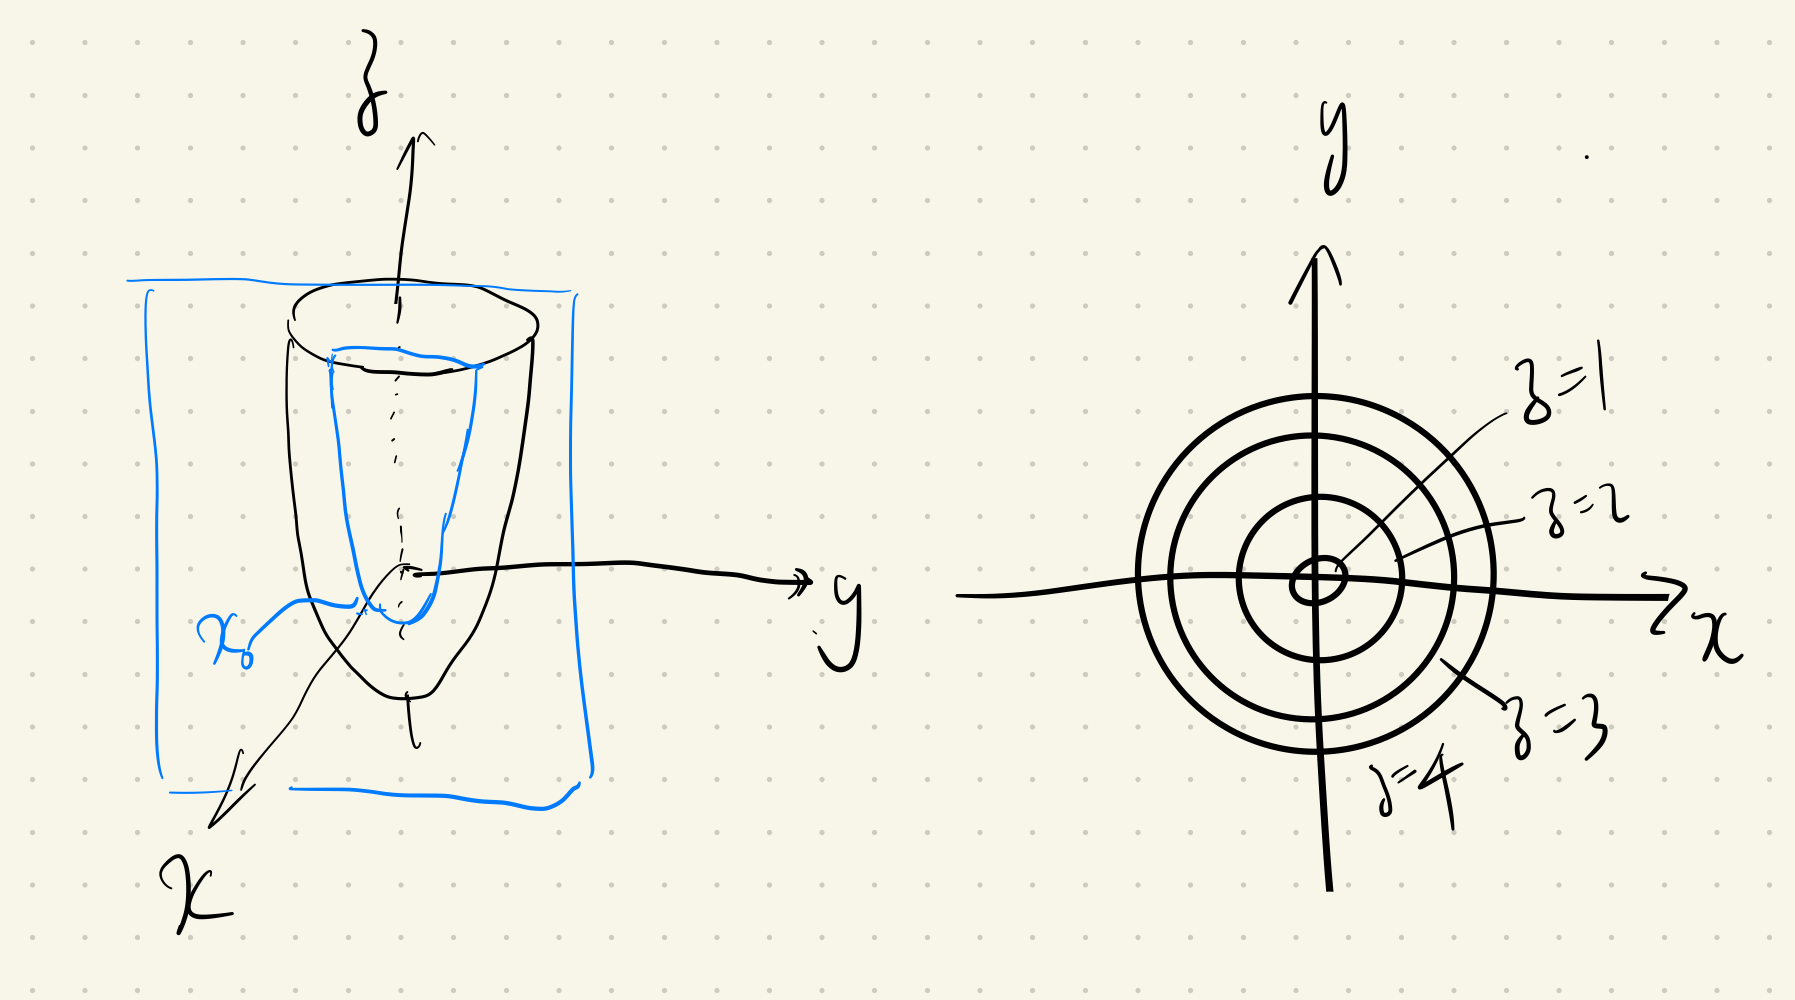
\includegraphics[width = 0.7\textwidth]{figures/chap 08/3D-graph.png}
\end{figure}

\section{Partial derivatives}
When we were dealing with univariable functions, we used derivatives to evaluate the slope of their tangent lines at a certain point, which reflects the rate of change of these functions at that very point.  In functions of two variables, we can still try to evaluate the rate of change of these functions.  What is different from univariable functions is that, for a univariable function, say, $f(x)$, when we are moving a tiny bit away from $(x_0, f(x_0))$, we can only go to $(x_0 + \delta x, f(x_0+ \delta x))$ or $(x_0 - \delta x, f(x_0 - \delta x))$, both of which have the same rate of change relative to $(x_0, f(x_0))$ as long as $f(x)$ is continuous.  However, for a function of two variables, say, $g(x,y)$, for every point on the surface $(x_0, y_0, f(x_0, y_0))$, there are countless direction we can move away from this point, and each direction would have a different rate of change.  

For example, suppose $g(x,y) = x^2 - xy$, and we are trying to find the derivative of $g$ at $(x,y) = (1,2)$.  In the calculation of the derivative, if we are moving away from $(1,2)$ along the direction parallel to $x$-axis, then we are essentially fixing the $y$-coordinate at $2$ while moving the $x$-coordinate.  Therefore, the trace of our movement would be on the plane $y=2$ with $z = g(x,2) = x^2 - 2x$, and the derivative would be 
\[\frac{d}{dx}g(x,0)\Big|_{x=1} = 2x-2|_{x=1} = 0\]
In contrast, if we are moving away from $(1,2)$ along the parallel the $y$-axis, then we are fixing the $x$-coordinate at $1$ while moving the $y$-coordinate.  So the trace of our movement would be on the plane $x=1$ with $z = g(1,y) = 1-y$, and the derivative would be
\[\frac{d}{dy}g(1,y)\Big|_{y=2} = -1|_{y=2} = -1\] 
We can see that moving toward different directions can give us different values of the derivative.  Therefore, before we evaluate the derivative of a function of two variables, we have to specify which direction we are moving away from the point of interest.  Two most obvious directions, as we have demonstrated above, are along the direction parallel to the $x$-axis (holding the $y$-coordinate as constant) and along the direction parallel to the $y$-axis (holding the $x$-coordinate as constant).  These directions lead to the two first-order partial derivatives of the function, defined as below:

\begin{defi}[Partial Derivatives of Functions of Two Variables]{def: partial}
    Let $f(x,y)$ be a continous function, then the first partial derivative of $f$ with respect to $x$ and $y$ are defined as
    \begin{align*}
        \frac{\p f}{\p x} := f_x(x,y) &:= \lim_{h \rightarrow 0} \frac{f(x+h,y)-f(x,y)}{h}\\
        \frac{\p f}{\p y} := f_y(x, y) &:= \lim_{h \rightarrow 0} \frac{f(x,y+h)-f(x,y)}{h}
    \end{align*}
    And the value of the partial derivatives at $(x_0, y_0)$ are denoted as
    \[\frac{\p f}{\p x}\Big|_{(x_0,y_0)} := f_x(x_0, y_0) \qquad\qquad \frac{\p f}{\p y}\Big|_{(x_0,y_0)} := f_y(x_0, y_0)\] 
\end{defi}

Although the definition of partial derivatives seems cumbersome, luckily, the way to derive them is simple: treat the input that is not to be differentiated as constant.  For example, previously we had $g(x, y) = x^2-xy$.  To derive $\p g/\p x$ and its value at $(1,2)$, we can then treat $y$ as a "constant" and differentiate with respect to $y$, which yields
\[\frac{\partial g}{\partial x} = 2x - y \qquad \frac{\partial g}{\partial x}\Big|_{(1,2)} = 2 \cdot 1 - 2 = 0\]
Likewise, we can derive the derivative at $(1,2)$ in the direction parallel to the $y$-axis by
\[\frac{\partial g}{\partial y} = 0 - x = -x \qquad \frac{\partial g}{\partial y}\Big|_{(1,2)} = -1\]
Both values for partial derivatives are exactly what we have derived previously.  We will further demonstrate how first-order partial derivatives are evaluated in the following examples:

\begin{eg}[]{eg: first_partial}
    Suppose a surface in a three-dimensionsal space can be described by $z = f(x,y) = (xy)^x$.
    \begin{enumerate}[a)]
        \item Find the first-order partial derivatives of $f$ with respect to $x$ and $y$.
        \item Evaluate the slope of $f(x,y)$ at $(1,e)$ in the direction parallel to the $x$-axis.
    \end{enumerate}
\end{eg}

\begin{egsol}[]{eg: first_partial}
    \begin{enumerate}[a)]
        \item For the partial derivative with respect to $x$, we try $y$ as "constant" and yield
        \begin{align*}
            \frac{\p f}{\p x} = \frac{\p}{\p x} (xy)^x&= \frac{\p}{\p x} (e^{\ln(xy)})^x &\\
            &= \frac{\p}{\p x} e^{x \ln(xy)}&\\
            &= e^{x \ln(xy)} \frac{\p}{\p x} (x \ln (xy))&\text{(Chain rule)}\\
            &= (xy)^x \Big[\ln(xy) + x \cdot \frac{1}{x}\Big]&\text{(Product rule)}\\
            &= (xy)^x(\ln(xy)+1)& 
        \end{align*}
        Likewise, for the partial derivative with respect to $y$:
        \[\frac{\p f}{\p y} = \frac{\p}{\p y}(xy)^x = \frac{\p}{\p y} x^x y^x = x^x \cdot x \cdot y^{x-1} = x^{x+1}y^{x-1}\]
        \item The slope of $f(x,y)$ at $(1,e)$ in the direction parallel to the $x$-axis is exactly the definition of $f_x(1,e)$, which can be evaluated by
        \[\frac{\p f}{\p x}\Big|_{(1,e)} = (1 \cdot e)^1 (\ln(1 \cdot e) + 1) = e \cdot (1+1) = 2e\]
    \end{enumerate}
\end{egsol}

\begin{ex}[]{ex: first_partial}
    Let the demand functions for two products $A$ and $B$, denoted as $q_A(p_A, p_B)$ and $q_B(p_A, p_B)$, be functions of the price of A ($p_A$) and price of B ($p_B$).  The two products are said to be \textit{complemetary} when 
    \[\frac{\p q_A}{\p p_B} < 0 \qquad \text{and} \qquad \frac{\p q_B}{\p p_A} < 0\]
    The two products are said to be \textit{substitutes} when 
    \[\frac{\p q_A}{\p p_B} > 0 \qquad \text{and} \qquad \frac{\p q_B}{\p p_A} > 0\]
    Suppose now we have 
    \begin{align*}
        q_A &= 180 - 2.5 p_A + 3 p_B\\
        q_B &= 200 + 1.5 p_A - 0.5 p_B 
    \end{align*}
    Determine if $A$ and $B$ are complementary, substitutes, or neither.
\end{ex}

\begin{exsol}[]{exsol: first_partial}
    Based on the definition of $q_A$ and $q_B$, we have the following partial derivatives:
    \begin{align*}
        \frac{\p q_A}{\p p_B} &= 3\\
        \frac{\p q_B}{\p p_A} &= 1.5
    \end{align*}
    Since both partial derivatives are positive, $A$ and $B$ are \textit{complementary}. 
\end{exsol}

In Definition \ref{def: partial}, we only defined the partial derivatives for functions of two variables.  This definition can be readily extended to functions of arbitrary number of variables as follows:

\begin{defi}[Partial Derivatives of Functions of Several Variables]{}
    Let $f(x_1, x_2, ..., x_p)$ be a continous function, then the first partial derivative of $f$ with respect to $x_j$ is defined as
    \[\frac{\p f}{\p x_j} := \lim_{h \rightarrow 0} \frac{f(x_1, x_2, ..., x_{j-1}, x_j+h, x_{j+1}, ... ,x_p)-f(x_1, x_2, ..., x_{j-1}, x_j, x_{j+1}, ... ,x_p)}{h}\]
\end{defi}

The recipe for deriving the partial derivative is exactly the same: treat all variables other than $x_j$ as constant and differentiate the function with respect to $x_j$.  For example, suppose we have $f(x,y,z,t) = xyz + yzt^2 + e^{xzt}$, then the partial derivative of $f$ with respect to $x$ is 
\[\frac{\p f}{\p x} = yz + 0 + e^{xzt} \cdot zt = yz + zte^{xzt}\]

Up until now, we have shown how to evaluate the first-order partial derivatives for functions of several variables.  As with ordinary derivatives, it also possible to do partial differentiation repeatedly to a function to obtain its higher-order partial derivatives.  However, note that since we have severval variables available for partial differentiation, we have to specify which variables and in what order do we want to carry out the partial differentiations.  For example, for a function of two variables $f(x,y)$, there are four ways to take its second-order partial derivative, defined with the notations below:

\begin{align*}
    &\frac{\p}{\p x}\Big(\frac{\p f}{\p x}\Big) := \frac{\p^2 f}{\p x^2} := f_{xx} := (f_x)_x \qquad 
    &\frac{\p}{\p y}\Big(\frac{\p f}{\p x}\Big) := \frac{\p^2 f}{\p y \p x} := f_{xy} := (f_x)_y\\
    &\frac{\p}{\p y}\Big(\frac{\p f}{\p y}\Big) := \frac{\p^2 f}{\p y^2} := f_{yy} := (f_y)_y \qquad &\frac{\p}{\p x}\Big(\frac{\p f}{\p y}\Big) := \frac{\p^2 f}{\p x \p y} := f_{yx} := (f_y)_x
    \\
\end{align*}

The two partial derivatives on the right are called \textit{mixed partial derivatives} since they take partial derivatives of different variables.  Notice that the order of $x$ and $y$ in the "fraction style" notation and "subscript style" notation are different: in the "fraction style" you differentiate in a right-to-left fashion, while in the "subscript style" notation you differentiate in a left-to-right fashion.  This may seem a little bit confusing, but fortunately, \textit{it can be shown that as long as the function has continuous second partial derivatives, the order of partial differentiation does not matter}.  To demonstrate this, lets suppose $f(x,y) = x^2y + xy^3$, then we have
\begin{align*}
    \frac{\p^2 f}{\p x^2} &= \frac{\p}{\p x}\Big(\frac{\p f}{\p x}\Big) = \frac{\p}{\p x}\Big(2xy + y^3\Big) = 2y\\
    \frac{\p^2 f}{\p y^2} &= \frac{\p}{\p y}\Big(\frac{\p f}{\p y}\Big) = \frac{\p}{\p y}\Big(x^2 + 3xy^2\Big) = 6xy\\
    \frac{\p^2 f}{\p y \p x} &= \frac{\p}{\p y}\Big(\frac{\p f}{\p x}\Big) = \frac{\p}{\p y}\Big(2xy + y^3\Big) = 2x + 3y^2\\
    \frac{\p^2 f}{\p x \p y} &= \frac{\p}{\p x}\Big(\frac{\p f}{\p y}\Big) = \frac{\p}{\p x}\Big(x^2 + 3xy^2\Big) = 2x + 3y^2
\end{align*}
which verifies that $f_{xy} = f_{yx}$.

\section{Extrema of Functions of Two Variables}

In single variable calculus, we used derivatives extensively to find the local and global extrema of a function.  For a brief recap, to find all the local extrema for a function $f(x)$, we argued that all local extrema should occur at the \textit{critical points} of the function, which is defined as points where its first derivative $f'(x) = 0$ or does not exist.  Therefore, we find all critical points of the function and check them one-by-one to see if they are local minima, local maxima, or neither.  In the case where a critical point is found by $f'(x) = 0$, we can use the \textit{first derivative test} or \textit{second derivative test} to help us do the checking.  In particular, the second derivative test states that a critical point $x = x_0$ attains local minimum if the second derivative $f''(x_0) > 0$, local maximum if $f''(x_0) < 0$, and no information is available from second derivative if $f''(x_0) = 0$.  Lastly, to find global extrema, we may find all local extrema and compare their function values with the function values at the boundary of the function's domain.  In this section, we will see that can can find the extrema of functions of two variables using methods analogus to what we have done in single variable calculus.

For the sake of completeness, we first provide a formal definition of global and local extrema for functions of two variables: 

\smallskip

\begin{defi}[Extrema of functions of two variables]{def: extrema_multi}
    Suppose $(x_0, y_0)$ is in the domain of $f(x,y)$, let $R_0$ be an region for input where $(x_0, y_0) \in R_0$
    \begin{itemize}
        \item $f$ has a \textbf{global (absolute) maximum} at $(x_0, y_0)$ in $R_0$ if $f(x,y) \le f(x_0,y_0), \forall x \in R_0$ 
        \item $f$ has a \textbf{global (absolute) minimum} at $(x_0, y_0)$ in $R_0$ if $f(x,y) \ge f(x_0,y_0), \forall x \in R_0$ 
        \item $f$ has a \textbf{local (relative) maximum} at $(x_0, y_0))$ in $I_0$ if there exists an circular region $R \subset R_0$ where $(x_0, y_0) \in R$ and $f(x,y) \le f(x_0, y_0), \forall x \in R$ 
        \item $f$ has a \textbf{local (relative) minimum} at $(x_0, y_0))$ in $I_0$ if there exists an circular region $R \subset R_0$ where $(x_0, y_0) \in R$ and $f(x,y) \ge f(x_0, y_0), \forall x \in R$ 
    \end{itemize}
\end{defi}

We can see that based on this definition, a local maximum is like a peak of a mountain, and a local minimum is like a valley.  To make sure that a point $(x_0,y_0)$ attains local maximum for a function $f(x,y)$, we must make sure that points neighboring $(x_0, y_0)$ \textit{at all directions} do not attain greater function value than $(x_0, y_0)$.  We now state the equivalent of Fermat's Interior Extremum Theorem for functions of two variables:

\begin{theo}[Interior Extremum Theorem for Functions of Two Variables]{thm: fermat_multi}
    Suppose $f(x, y)$ attains local extremum at $(x_0, y_0) \in R$, where $R$ is an open region.  If the first partial derivatives of $f(x,y)$ exists in $R$, then $f_x(x_0, y_0) = f_y(x_0, y_0) = 0$.
\end{theo}

The intuition of this theorem is that, if you see $f(x, y)$ as a geographic map measuring the height of each point, then as long as the terrain is smooth (existence of first partial derivatives) within a certain area of the map ($R$), then if you are at a valley or a peak, the ground will be relatively flat at where you stand (zero partial derivative).  However, the converse is not true: when the ground is relative flat near you, it is possible that you are neither at a peak nor a valley.  For example, it is possible that you ascend when you walk forwards and backwards, but descend when you walk to the left or right, which is the case for the point marked as X in the following graph.  This kind of point, where the two partial derivatives evaluate to zero but deos not attain local extremum, is called a \textbf{saddle point}.

\begin{center}
    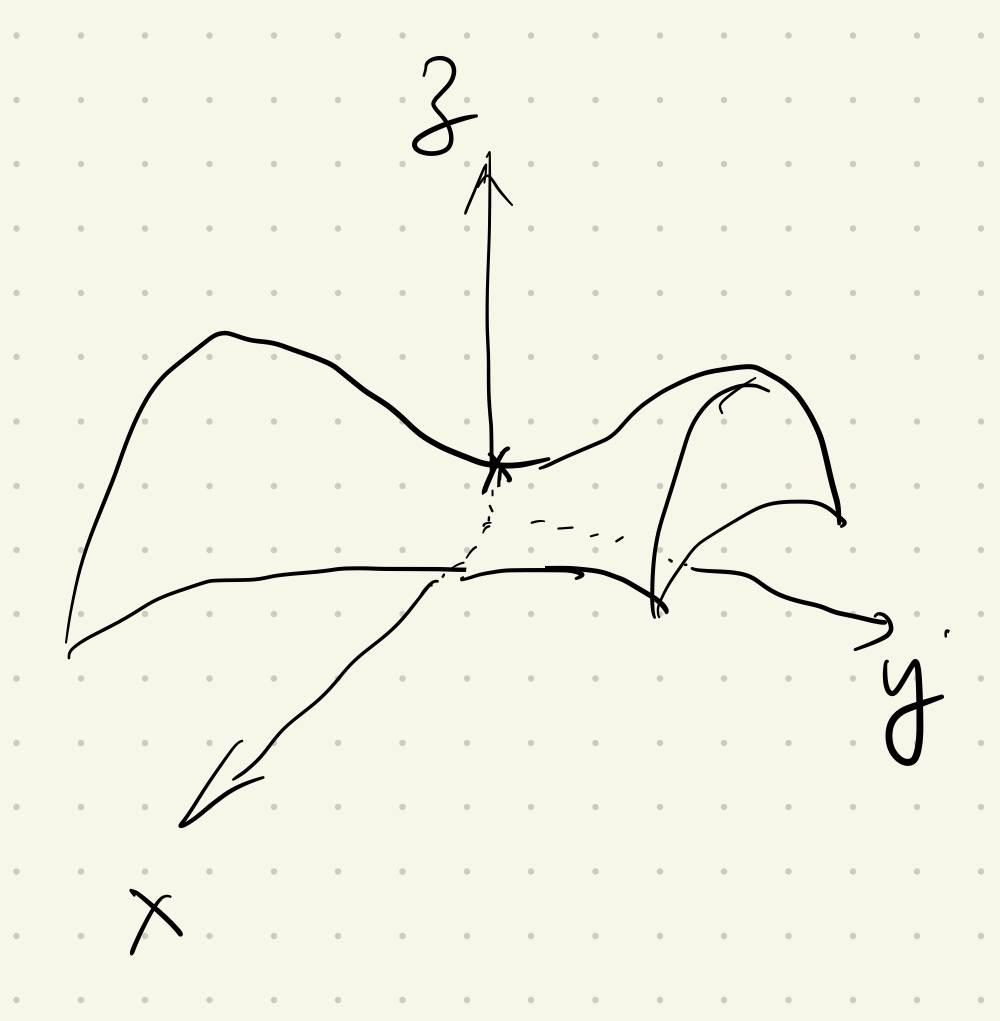
\includegraphics[width = 0.4\textwidth]{figures/chap 08/saddle.png}
\end{center}

Since all local extrema occur at where both partial derivatives evaluates to zero when both partial derivatives exist, we can define critical points of functions of two variables as follows, in order to capture all possible points that can attain local extrema:

\begin{defi}[Critical points of functions of two variables]{def: crit}
    A point $(x_0, y_0)$ in the domain of $f(x, y)$ is termed as a \textit{critical point} for $f(x, y)$ if either of the following holds:
    \begin{enumerate}
        \item $f_x(x_0, y_0) = f_y(x_0, y_0) = 0$
        \item $f_x(x_0, y_0)$ or $f_y(x_0, y_0)$ is undefined at $(x_0, y_0)$
    \end{enumerate}
\end{defi}

After finding the critical points for a function, aside from trying to plot the function around the critical points to assess its behavior at these points, we can use the following second partial derivative test to help us categorize the critical points as long as they are found by letting $f_x(x,y) = f_y(x,y) = 0$.

\begin{theo}[Second Partial Derivative Test for Relative Extrema]{thm: second_partial}
    Suppose a function $f(x, y)$ has continuous second partial derivatives in a region $R$ containing $(x_0, y_0)$ where $f_x(x_0, y_0) = f_y(x_0, y_0) = 0$.  Define the determinant $D$ as
    \[D = f_{xx}(x_0, y_0)f_{yy}(x_0, y_0) - [f_{xy}(x_0, y_0)]^2\]
    \begin{enumerate}
        \item If $D > 0$, then $f$ has a local extrema at $(x_0,y_0)$, and we assess the sign of $f_xx(x_0,y_0)$.
        \begin{enumerate}
            \item If $f_{xx}(x_0,y_0) > 0$, $f$ attains \textbf{local minimum} at $(x_0, y_0)$.
            \item If $f_{xx}(x_0,y_0) < 0$, $f$ attains \textbf{local maxmimum} at $(x_0, y_0)$.
        \end{enumerate}
        \item If $D < 0$, then $(x_0, y_0)$ is a \textbf{saddle point}.
        \item If $D = 0$, the second partial derivatives give no information.
    \end{enumerate}
\end{theo}

Here we will not show how $D$ is derived, but will provide some intuition on why this criterion is needed and why it makes sense.  When $f_{xx}(x_0,y_0)$ and $f_{yy}(x_0,y_0)$ have opposite signs, we can see that $D$ is guaranteed to be less than zero and $(x_0, y_0)$ is a saddle point.  This is reasonable since in the case where $f_{xx}(x_0,y_0) > 0$ and $f_{yy}(x_0,y_0) <0$, the trace of the surface is concave up on $y = y_0$ and concave down on $x = x_0$, which implies that when you are walking from $(x_0, y_0)$, the terrain ascends when you walk parallel to the $x$-axis but decends when you walk parallel to the $y$-axis.  Therefore, it is clear that this point is niether a valley or a peak, so it is a saddle point.  The situtation is similar when $f_{xx}(x_0,y_0) < 0$ and $f_{yy}(x_0,y_0) > 0$.


When both $f_{xx}(x_0,y_0)$ and $f_{yy}(x_0,y_0)$ are positive, the traces of the surface on $x = x_0$ and $y = y_0$ are both concave up, which implies that when you stand at $(x_0, y_0)$ and walk parallel to either the $x$- or $y$-axis, you will find the terrain ascending.  However, this is not sufficient to prove that you are in a valley (i.e. local minimum) since you are still not sure if the terrain would be descending when you walk in a direction not parellel to either the $x$- or $y$-axis.  The additional mixed partial derivative term $[f_{xy}(x_0, y_0)]^2$ can be seen as to provide information on what would happen if you walked diagonally.  When it is large enough to offset the $f_{xx}(x_0,y_0)f_{yy}(x_0,y_0)$ and make $D$ negative, this implies that there are some walking directions where the terrain becomes descending, and the point becomes a saddle point.  Similar arguments can be made in the case where $f_{xx}(x_0,y_0)$ and $f_{yy}(x_0,y_0)$ are both negative.

We will now see how the series of procedures above works in finding local extrema:

\begin{eg}[]{eg: extrema_multi}

\end{eg}

%\bibliography{bibfile}

\end{document}